\documentclass[twoside]{book}

% Packages required by doxygen
\usepackage{fixltx2e}
\usepackage{calc}
\usepackage{doxygen}
\usepackage[export]{adjustbox} % also loads graphicx
\usepackage{graphicx}
\usepackage[utf8]{inputenc}
\usepackage{makeidx}
\usepackage{multicol}
\usepackage{multirow}
\PassOptionsToPackage{warn}{textcomp}
\usepackage{textcomp}
\usepackage[nointegrals]{wasysym}
\usepackage[table]{xcolor}

% Font selection
\usepackage[T1]{fontenc}
\usepackage[scaled=.90]{helvet}
\usepackage{courier}
\usepackage{amssymb}
\usepackage{sectsty}
\renewcommand{\familydefault}{\sfdefault}
\allsectionsfont{%
  \fontseries{bc}\selectfont%
  \color{darkgray}%
}
\renewcommand{\DoxyLabelFont}{%
  \fontseries{bc}\selectfont%
  \color{darkgray}%
}
\newcommand{\+}{\discretionary{\mbox{\scriptsize$\hookleftarrow$}}{}{}}

% Page & text layout
\usepackage{geometry}
\geometry{%
  a4paper,%
  top=2.5cm,%
  bottom=2.5cm,%
  left=2.5cm,%
  right=2.5cm%
}
\tolerance=750
\hfuzz=15pt
\hbadness=750
\setlength{\emergencystretch}{15pt}
\setlength{\parindent}{0cm}
\setlength{\parskip}{3ex plus 2ex minus 2ex}
\makeatletter
\renewcommand{\paragraph}{%
  \@startsection{paragraph}{4}{0ex}{-1.0ex}{1.0ex}{%
    \normalfont\normalsize\bfseries\SS@parafont%
  }%
}
\renewcommand{\subparagraph}{%
  \@startsection{subparagraph}{5}{0ex}{-1.0ex}{1.0ex}{%
    \normalfont\normalsize\bfseries\SS@subparafont%
  }%
}
\makeatother

% Headers & footers
\usepackage{fancyhdr}
\pagestyle{fancyplain}
\fancyhead[LE]{\fancyplain{}{\bfseries\thepage}}
\fancyhead[CE]{\fancyplain{}{}}
\fancyhead[RE]{\fancyplain{}{\bfseries\leftmark}}
\fancyhead[LO]{\fancyplain{}{\bfseries\rightmark}}
\fancyhead[CO]{\fancyplain{}{}}
\fancyhead[RO]{\fancyplain{}{\bfseries\thepage}}
\fancyfoot[LE]{\fancyplain{}{}}
\fancyfoot[CE]{\fancyplain{}{}}
\fancyfoot[RE]{\fancyplain{}{\bfseries\scriptsize Generated by Doxygen }}
\fancyfoot[LO]{\fancyplain{}{\bfseries\scriptsize Generated by Doxygen }}
\fancyfoot[CO]{\fancyplain{}{}}
\fancyfoot[RO]{\fancyplain{}{}}
\renewcommand{\footrulewidth}{0.4pt}
\renewcommand{\chaptermark}[1]{%
  \markboth{#1}{}%
}
\renewcommand{\sectionmark}[1]{%
  \markright{\thesection\ #1}%
}

% Indices & bibliography
\usepackage{natbib}
\usepackage[titles]{tocloft}
\setcounter{tocdepth}{3}
\setcounter{secnumdepth}{5}
\makeindex

% Hyperlinks (required, but should be loaded last)
\usepackage{ifpdf}
\ifpdf
  \usepackage[pdftex,pagebackref=true]{hyperref}
\else
  \usepackage[ps2pdf,pagebackref=true]{hyperref}
\fi
\hypersetup{%
  colorlinks=true,%
  linkcolor=blue,%
  citecolor=blue,%
  unicode%
}

% Custom commands
\newcommand{\clearemptydoublepage}{%
  \newpage{\pagestyle{empty}\cleardoublepage}%
}

\usepackage{caption}
\captionsetup{labelsep=space,justification=centering,font={bf},singlelinecheck=off,skip=4pt,position=top}

%===== C O N T E N T S =====

\begin{document}

% Titlepage & ToC
\hypersetup{pageanchor=false,
             bookmarksnumbered=true,
             pdfencoding=unicode
            }
\pagenumbering{alph}
\begin{titlepage}
\vspace*{7cm}
\begin{center}%
{\Large Blaze \\[1ex]\large 0.\+1 }\\
\vspace*{1cm}
{\large Generated by Doxygen 1.8.13}\\
\end{center}
\end{titlepage}
\clearemptydoublepage
\pagenumbering{roman}
\tableofcontents
\clearemptydoublepage
\pagenumbering{arabic}
\hypersetup{pageanchor=true}

%--- Begin generated contents ---
\chapter{Deprecated List}
\label{deprecated}
\Hypertarget{deprecated}

\begin{DoxyRefList}
\item[\label{deprecated__deprecated000001}%
\Hypertarget{deprecated__deprecated000001}%
Member \hyperlink{classblaze_1_1Context_adecff6f1105733085198f877aa04e78f}{blaze\+:\+:Context\+:\+:create\+Image} (uint32\+\_\+t width, uint32\+\_\+t height, uint32\+\_\+t miplevels, Vk\+Format format, Vk\+Image\+Tiling tiling, Vk\+Image\+Usage\+Flags vulkan\+Usage, Vma\+Memory\+Usage vma\+Usage) const]Since layers were added.
\end{DoxyRefList}
\chapter{Module Index}
\section{Modules}
Here is a list of all modules\+:\begin{DoxyCompactList}
\item \contentsline{section}{Uniform\+Buffer\+Objects}{\pageref{group__UniformBufferObjects}}{}
\item \contentsline{section}{Push\+Constant\+Blocks}{\pageref{group__PushConstantBlocks}}{}
\end{DoxyCompactList}

\chapter{Namespace Index}
\section{Namespace List}
Here is a list of all documented namespaces with brief descriptions\+:\begin{DoxyCompactList}
\item\contentsline{section}{\hyperlink{namespaceblaze}{blaze} \\*Main namespace for the blaze project }{\pageref{namespaceblaze}}{}
\item\contentsline{section}{\hyperlink{namespaceblaze_1_1util}{blaze\+::util} \\*Contains all the utility classes and functions used in Blaze }{\pageref{namespaceblaze_1_1util}}{}
\item\contentsline{section}{\hyperlink{namespaceblaze_1_1vkw}{blaze\+::vkw} \\*The namespace for all the vulkan managed wrapper classes }{\pageref{namespaceblaze_1_1vkw}}{}
\item\contentsline{section}{\hyperlink{namespaceblaze_1_1vkw_1_1base}{blaze\+::vkw\+::base} \\*A namespace used to hold the Vk\+Wrap structs to avoid random usage from outside the Vk\+Wrap internals }{\pageref{namespaceblaze_1_1vkw_1_1base}}{}
\end{DoxyCompactList}

\chapter{Hierarchical Index}
\section{Class Hierarchy}
This inheritance list is sorted roughly, but not completely, alphabetically\+:\begin{DoxyCompactList}
\item \contentsline{section}{blaze\+:\+:A\+Renderer}{\pageref{classblaze_1_1ARenderer}}{}
\begin{DoxyCompactList}
\item \contentsline{section}{blaze\+:\+:Fwd\+Renderer}{\pageref{classblaze_1_1FwdRenderer}}{}
\end{DoxyCompactList}
\item \contentsline{section}{blaze\+:\+:spirv\+:\+:Attachment\+Format}{\pageref{structblaze_1_1spirv_1_1AttachmentFormat}}{}
\item \contentsline{section}{blaze\+:\+:util\+:\+:Auto\+Timer}{\pageref{classblaze_1_1util_1_1AutoTimer}}{}
\item \contentsline{section}{blaze\+:\+:vkw\+:\+:base\+:\+:Base\+Collection$<$ T\+Handle $>$}{\pageref{structblaze_1_1vkw_1_1base_1_1BaseCollection}}{}
\item \contentsline{section}{blaze\+:\+:Base\+U\+BO}{\pageref{classblaze_1_1BaseUBO}}{}
\begin{DoxyCompactList}
\item \contentsline{section}{blaze\+:\+:U\+BO$<$ T $>$}{\pageref{classblaze_1_1UBO}}{}
\item \contentsline{section}{blaze\+:\+:U\+BO$<$ blaze\+:\+:Cascade\+U\+Block $>$}{\pageref{classblaze_1_1UBO}}{}
\item \contentsline{section}{blaze\+:\+:U\+BO$<$ blaze\+:\+:Shadow\+U\+Block $>$}{\pageref{classblaze_1_1UBO}}{}
\end{DoxyCompactList}
\item \contentsline{section}{blaze\+:\+:Base\+V\+BO}{\pageref{classblaze_1_1BaseVBO}}{}
\begin{DoxyCompactList}
\item \contentsline{section}{blaze\+:\+:Index\+Buffer$<$ T $>$}{\pageref{classblaze_1_1IndexBuffer}}{}
\item \contentsline{section}{blaze\+:\+:Vertex\+Buffer$<$ T $>$}{\pageref{classblaze_1_1VertexBuffer}}{}
\item \contentsline{section}{blaze\+:\+:Index\+Buffer$<$ uint32\+\_\+t $>$}{\pageref{classblaze_1_1IndexBuffer}}{}
\item \contentsline{section}{blaze\+:\+:Vertex\+Buffer$<$ blaze\+:\+:Vertex $>$}{\pageref{classblaze_1_1VertexBuffer}}{}
\end{DoxyCompactList}
\item \contentsline{section}{blaze\+:\+:vkw\+:\+:base\+:\+:Base\+Wrapper$<$ T\+Handle $>$}{\pageref{structblaze_1_1vkw_1_1base_1_1BaseWrapper}}{}
\item \contentsline{section}{blaze\+:\+:Bindable}{\pageref{classblaze_1_1Bindable}}{}
\begin{DoxyCompactList}
\item \contentsline{section}{blaze\+:\+:util\+:\+:Environment}{\pageref{classblaze_1_1util_1_1Environment}}{}
\end{DoxyCompactList}
\item \contentsline{section}{blaze\+:\+:Buffer\+Object}{\pageref{structblaze_1_1BufferObject}}{}
\item \contentsline{section}{blaze\+:\+:Camera}{\pageref{classblaze_1_1Camera}}{}
\item \contentsline{section}{blaze\+:\+:Camera\+Control\+Info}{\pageref{structblaze_1_1CameraControlInfo}}{}
\item \contentsline{section}{blaze\+:\+:Camera\+U\+Block}{\pageref{structblaze_1_1CameraUBlock}}{}
\item \contentsline{section}{blaze\+:\+:Cascade\+Block}{\pageref{structblaze_1_1CascadeBlock}}{}
\item \contentsline{section}{Cascade\+Shadow\+Uniform\+Buffer\+Object}{\pageref{structCascadeShadowUniformBufferObject}}{}
\item \contentsline{section}{blaze\+:\+:Cascade\+U\+Block}{\pageref{structblaze_1_1CascadeUBlock}}{}
\item \contentsline{section}{blaze\+:\+:vkw\+:\+:Command\+Buffer\+Vector}{\pageref{structblaze_1_1vkw_1_1CommandBufferVector}}{}
\item \contentsline{section}{blaze\+:\+:Context}{\pageref{classblaze_1_1Context}}{}
\item \contentsline{section}{blaze\+:\+:Cubemap\+U\+Block}{\pageref{structblaze_1_1CubemapUBlock}}{}
\item \contentsline{section}{blaze\+:\+:util\+:\+:Debug\+Counts}{\pageref{structblaze_1_1util_1_1DebugCounts}}{}
\item \contentsline{section}{blaze\+:\+:Debug\+Render\+Settings}{\pageref{structblaze_1_1DebugRenderSettings}}{}
\item \contentsline{section}{blaze\+:\+:vkw\+:\+:base\+:\+:Dependent\+Holder$<$ T\+Handle, T\+Dep, T\+Destroy $>$}{\pageref{structblaze_1_1vkw_1_1base_1_1DependentHolder}}{}
\item \contentsline{section}{blaze\+:\+:vkw\+:\+:base\+:\+:Device\+Dependent\+Vector$<$ T\+Handle, T\+Destroy $>$}{\pageref{structblaze_1_1vkw_1_1base_1_1DeviceDependentVector}}{}
\item \contentsline{section}{Directional\+Shadow}{\pageref{classDirectionalShadow}}{}
\item \contentsline{section}{blaze\+:\+:Drawable}{\pageref{classblaze_1_1Drawable}}{}
\begin{DoxyCompactList}
\item \contentsline{section}{blaze\+:\+:Model}{\pageref{classblaze_1_1Model}}{}
\item \contentsline{section}{blaze\+:\+:Model2}{\pageref{classblaze_1_1Model2}}{}
\end{DoxyCompactList}
\item \contentsline{section}{blaze\+:\+:spirv\+:\+:Shader\+:\+:Set\+:\+:Format}{\pageref{structblaze_1_1spirv_1_1Shader_1_1Set_1_1Format}}{}
\item \contentsline{section}{blaze\+:\+:spirv\+:\+:Framebuffer\+:\+:Format}{\pageref{structblaze_1_1spirv_1_1Framebuffer_1_1Format}}{}
\item \contentsline{section}{blaze\+:\+:spirv\+:\+:Framebuffer}{\pageref{structblaze_1_1spirv_1_1Framebuffer}}{}
\item \contentsline{section}{blaze\+:\+:spirv\+:\+:Graphics\+Pipeline\+Create\+Info}{\pageref{structblaze_1_1spirv_1_1GraphicsPipelineCreateInfo}}{}
\item \contentsline{section}{blaze\+:\+:G\+UI}{\pageref{classblaze_1_1GUI}}{}
\item \contentsline{section}{blaze\+:\+:Image\+Data2D}{\pageref{structblaze_1_1ImageData2D}}{}
\item \contentsline{section}{blaze\+:\+:Image\+Data\+Cube}{\pageref{structblaze_1_1ImageDataCube}}{}
\item \contentsline{section}{blaze\+:\+:Image\+Object}{\pageref{structblaze_1_1ImageObject}}{}
\item \contentsline{section}{blaze\+:\+:vkw\+:\+:base\+:\+:Independent\+Holder$<$ T\+Handle, T\+Destroy $>$}{\pageref{structblaze_1_1vkw_1_1base_1_1IndependentHolder}}{}
\item \contentsline{section}{blaze\+:\+:Indexed\+Vertex\+Buffer$<$ T $>$}{\pageref{classblaze_1_1IndexedVertexBuffer}}{}
\item \contentsline{section}{blaze\+:\+:Indexed\+Vertex\+Buffer$<$ blaze\+:\+:Vertex $>$}{\pageref{classblaze_1_1IndexedVertexBuffer}}{}
\item \contentsline{section}{blaze\+:\+:Lights\+U\+Block}{\pageref{structblaze_1_1LightsUBlock}}{}
\item \contentsline{section}{blaze\+:\+:Light\+System}{\pageref{classblaze_1_1LightSystem}}{}
\item \contentsline{section}{blaze\+:\+:spirv\+:\+:Load\+Store\+Config}{\pageref{structblaze_1_1spirv_1_1LoadStoreConfig}}{}
\item \contentsline{section}{blaze\+:\+:util\+:\+:Managed$<$ T $>$}{\pageref{classblaze_1_1util_1_1Managed}}{}
\item \contentsline{section}{blaze\+:\+:util\+:\+:Managed$<$ blaze\+:\+:Image\+Object $>$}{\pageref{classblaze_1_1util_1_1Managed}}{}
\item \contentsline{section}{blaze\+:\+:util\+:\+:Managed$<$ Vk\+Descriptor\+Pool $>$}{\pageref{classblaze_1_1util_1_1Managed}}{}
\item \contentsline{section}{blaze\+:\+:util\+:\+:Managed$<$ Vk\+Descriptor\+Set\+Layout $>$}{\pageref{classblaze_1_1util_1_1Managed}}{}
\item \contentsline{section}{blaze\+:\+:util\+:\+:Managed$<$ Vk\+Image\+View $>$}{\pageref{classblaze_1_1util_1_1Managed}}{}
\item \contentsline{section}{blaze\+:\+:util\+:\+:Managed$<$ Vk\+Pipeline $>$}{\pageref{classblaze_1_1util_1_1Managed}}{}
\item \contentsline{section}{blaze\+:\+:util\+:\+:Managed$<$ Vk\+Pipeline\+Layout $>$}{\pageref{classblaze_1_1util_1_1Managed}}{}
\item \contentsline{section}{blaze\+:\+:util\+:\+:Managed$<$ Vk\+Render\+Pass $>$}{\pageref{classblaze_1_1util_1_1Managed}}{}
\item \contentsline{section}{blaze\+:\+:util\+:\+:Managed$<$ Vk\+Sampler $>$}{\pageref{classblaze_1_1util_1_1Managed}}{}
\item \contentsline{section}{blaze\+:\+:util\+:\+:Managed\+Vector$<$ T, singular $>$}{\pageref{classblaze_1_1util_1_1ManagedVector}}{}
\item \contentsline{section}{blaze\+:\+:util\+:\+:Managed\+Vector$<$ T, false $>$}{\pageref{classblaze_1_1util_1_1ManagedVector_3_01T_00_01false_01_4}}{}
\item \contentsline{section}{blaze\+:\+:util\+:\+:Managed\+Vector$<$ Vk\+Command\+Buffer, false $>$}{\pageref{classblaze_1_1util_1_1ManagedVector}}{}
\item \contentsline{section}{blaze\+:\+:util\+:\+:Managed\+Vector$<$ Vk\+Framebuffer $>$}{\pageref{classblaze_1_1util_1_1ManagedVector}}{}
\item \contentsline{section}{blaze\+:\+:util\+:\+:Managed\+Vector$<$ Vk\+Image\+View $>$}{\pageref{classblaze_1_1util_1_1ManagedVector}}{}
\item \contentsline{section}{blaze\+:\+:Material}{\pageref{classblaze_1_1Material}}{}
\item \contentsline{section}{blaze\+:\+:Model2\+:\+:Material}{\pageref{structblaze_1_1Model2_1_1Material}}{}
\item \contentsline{section}{blaze\+:\+:Material\+Push\+Constant\+Block}{\pageref{structblaze_1_1MaterialPushConstantBlock}}{}
\item \contentsline{section}{blaze\+:\+:vkw\+:\+:Mem\+Allocator}{\pageref{structblaze_1_1vkw_1_1MemAllocator}}{}
\item \contentsline{section}{blaze\+:\+:Model\+Loader}{\pageref{classblaze_1_1ModelLoader}}{}
\item \contentsline{section}{blaze\+:\+:Model\+Push\+Constant\+Block}{\pageref{structblaze_1_1ModelPushConstantBlock}}{}
\item \contentsline{section}{blaze\+:\+:Node}{\pageref{structblaze_1_1Node}}{}
\item \contentsline{section}{blaze\+:\+:util\+:\+:Packed\+Handler$<$ T $>$}{\pageref{classblaze_1_1util_1_1PackedHandler}}{}
\item \contentsline{section}{blaze\+:\+:util\+:\+:Packed\+Handler$<$ blaze\+:\+:Drawable $\ast$$>$}{\pageref{classblaze_1_1util_1_1PackedHandler}}{}
\item \contentsline{section}{blaze\+:\+:util\+:\+:Packed\+Handler$<$ Drawable $\ast$ $>$}{\pageref{classblaze_1_1util_1_1PackedHandler}}{}
\item \contentsline{section}{blaze\+:\+:Model2\+:\+:Material\+:\+:P\+CB}{\pageref{structblaze_1_1Model2_1_1Material_1_1PCB}}{}
\item \contentsline{section}{blaze\+:\+:spirv\+:\+:Pipeline}{\pageref{structblaze_1_1spirv_1_1Pipeline}}{}
\item \contentsline{section}{blaze\+:\+:spirv\+:\+:Pipeline\+Factory}{\pageref{classblaze_1_1spirv_1_1PipelineFactory}}{}
\item \contentsline{section}{Point\+Shadow}{\pageref{classPointShadow}}{}
\item \contentsline{section}{blaze\+:\+:Primitive}{\pageref{structblaze_1_1Primitive}}{}
\item \contentsline{section}{blaze\+:\+:util\+:\+:Process$<$ P\+CB $>$}{\pageref{classblaze_1_1util_1_1Process}}{}
\item \contentsline{section}{blaze\+:\+:spirv\+:\+:Shader\+:\+:Push\+Constant}{\pageref{structblaze_1_1spirv_1_1Shader_1_1PushConstant}}{}
\item \contentsline{section}{blaze\+:\+:util\+:\+:Queue\+Family\+Indices}{\pageref{structblaze_1_1util_1_1QueueFamilyIndices}}{}
\item \contentsline{section}{blaze\+:\+:Renderer}{\pageref{classblaze_1_1Renderer}}{}
\begin{DoxyCompactList}
\item \contentsline{section}{blaze\+:\+:Forward\+Renderer}{\pageref{classblaze_1_1ForwardRenderer}}{}
\end{DoxyCompactList}
\item \contentsline{section}{blaze\+:\+:Renderer\+U\+Block}{\pageref{structblaze_1_1RendererUBlock}}{}
\item \contentsline{section}{blaze\+:\+:spirv\+:\+:Render\+Pass}{\pageref{structblaze_1_1spirv_1_1RenderPass}}{}
\item \contentsline{section}{blaze\+:\+:spirv\+:\+:Shader\+:\+:Set}{\pageref{structblaze_1_1spirv_1_1Shader_1_1Set}}{}
\item \contentsline{section}{blaze\+:\+:spirv\+:\+:Set\+Singleton}{\pageref{structblaze_1_1spirv_1_1SetSingleton}}{}
\item \contentsline{section}{blaze\+:\+:Settings\+U\+Block}{\pageref{structblaze_1_1SettingsUBlock}}{}
\item \contentsline{section}{blaze\+:\+:spirv\+:\+:Set\+Vector}{\pageref{structblaze_1_1spirv_1_1SetVector}}{}
\item \contentsline{section}{blaze\+:\+:spirv\+:\+:Shader}{\pageref{structblaze_1_1spirv_1_1Shader}}{}
\item \contentsline{section}{blaze\+:\+:spirv\+:\+:Shader\+Stage\+Data}{\pageref{structblaze_1_1spirv_1_1ShaderStageData}}{}
\item \contentsline{section}{blaze\+:\+:Shadow\+Push\+Constant\+Block}{\pageref{structblaze_1_1ShadowPushConstantBlock}}{}
\item \contentsline{section}{blaze\+:\+:Shadow\+U\+Block}{\pageref{structblaze_1_1ShadowUBlock}}{}
\item \contentsline{section}{blaze\+:\+:Swapchain}{\pageref{classblaze_1_1Swapchain}}{}
\item \contentsline{section}{blaze\+:\+:util\+:\+:Swapchain\+Support\+Details}{\pageref{structblaze_1_1util_1_1SwapchainSupportDetails}}{}
\item \contentsline{section}{blaze\+:\+:util\+:\+:Texture2\+Cubemap\+Info$<$ P\+CB $>$}{\pageref{structblaze_1_1util_1_1Texture2CubemapInfo}}{}
\item \contentsline{section}{blaze\+:\+:Texture2D}{\pageref{classblaze_1_1Texture2D}}{}
\item \contentsline{section}{blaze\+:\+:Texture\+Cube}{\pageref{classblaze_1_1TextureCube}}{}
\item \contentsline{section}{blaze\+:\+:Debug\+Render\+Settings\+:\+:Texture\+View\+Menu\+Control}{\pageref{structblaze_1_1DebugRenderSettings_1_1TextureViewMenuControl}}{}
\item \contentsline{section}{blaze\+:\+:U\+B\+O\+Vector$<$ T $>$}{\pageref{classblaze_1_1UBOVector}}{}
\item \contentsline{section}{blaze\+:\+:U\+B\+O\+Vector$<$ Camera\+U\+Block $>$}{\pageref{classblaze_1_1UBOVector}}{}
\item \contentsline{section}{blaze\+:\+:spirv\+:\+:Uniform\+Info}{\pageref{structblaze_1_1spirv_1_1UniformInfo}}{}
\item \contentsline{section}{blaze\+:\+:util\+:\+:Unmanaged$<$ T $>$}{\pageref{classblaze_1_1util_1_1Unmanaged}}{}
\item \contentsline{section}{blaze\+:\+:util\+:\+:Unmanaged$<$ Vk\+Descriptor\+Set $>$}{\pageref{classblaze_1_1util_1_1Unmanaged}}{}
\item \contentsline{section}{blaze\+:\+:util\+:\+:Unmanaged\+Vector$<$ T $>$}{\pageref{classblaze_1_1util_1_1UnmanagedVector}}{}
\item \contentsline{section}{blaze\+:\+:Vertex}{\pageref{structblaze_1_1Vertex}}{}
\item \contentsline{section}{blaze\+:\+:Vertex\+Input\+Format}{\pageref{structblaze_1_1VertexInputFormat}}{}
\end{DoxyCompactList}

\chapter{Class Index}
\section{Class List}
Here are the classes, structs, unions and interfaces with brief descriptions\+:\begin{DoxyCompactList}
\item\contentsline{section}{\hyperlink{classblaze_1_1ARenderer}{blaze\+::\+A\+Renderer} }{\pageref{classblaze_1_1ARenderer}}{}
\item\contentsline{section}{\hyperlink{structblaze_1_1spirv_1_1AttachmentFormat}{blaze\+::spirv\+::\+Attachment\+Format} }{\pageref{structblaze_1_1spirv_1_1AttachmentFormat}}{}
\item\contentsline{section}{\hyperlink{classblaze_1_1util_1_1AutoTimer}{blaze\+::util\+::\+Auto\+Timer} }{\pageref{classblaze_1_1util_1_1AutoTimer}}{}
\item\contentsline{section}{\hyperlink{structblaze_1_1vkw_1_1base_1_1BaseCollection}{blaze\+::vkw\+::base\+::\+Base\+Collection$<$ T\+Handle $>$} \\*The basic collection wrapper for uniformity }{\pageref{structblaze_1_1vkw_1_1base_1_1BaseCollection}}{}
\item\contentsline{section}{\hyperlink{classblaze_1_1BaseUBO}{blaze\+::\+Base\+U\+BO} \\*The base class for all U\+B\+Os }{\pageref{classblaze_1_1BaseUBO}}{}
\item\contentsline{section}{\hyperlink{classblaze_1_1BaseVBO}{blaze\+::\+Base\+V\+BO} }{\pageref{classblaze_1_1BaseVBO}}{}
\item\contentsline{section}{\hyperlink{structblaze_1_1vkw_1_1base_1_1BaseWrapper}{blaze\+::vkw\+::base\+::\+Base\+Wrapper$<$ T\+Handle $>$} \\*The basic wrapper for uniformity }{\pageref{structblaze_1_1vkw_1_1base_1_1BaseWrapper}}{}
\item\contentsline{section}{\hyperlink{classblaze_1_1Bindable}{blaze\+::\+Bindable} }{\pageref{classblaze_1_1Bindable}}{}
\item\contentsline{section}{\hyperlink{structblaze_1_1BufferObject}{blaze\+::\+Buffer\+Object} \\*Simple holder for info on a buffer (handle and allocation) }{\pageref{structblaze_1_1BufferObject}}{}
\item\contentsline{section}{\hyperlink{classblaze_1_1Camera}{blaze\+::\+Camera} \\*Utility class enclosing the \hyperlink{classblaze_1_1UBO}{U\+BO} and associated calculations }{\pageref{classblaze_1_1Camera}}{}
\item\contentsline{section}{\hyperlink{structblaze_1_1CameraControlInfo}{blaze\+::\+Camera\+Control\+Info} }{\pageref{structblaze_1_1CameraControlInfo}}{}
\item\contentsline{section}{\hyperlink{structblaze_1_1CameraUBlock}{blaze\+::\+Camera\+U\+Block} \\*Holds camera data to be sent to G\+PU }{\pageref{structblaze_1_1CameraUBlock}}{}
\item\contentsline{section}{\hyperlink{structblaze_1_1CascadeBlock}{blaze\+::\+Cascade\+Block} \\*A struct to return cascaded shadow P\+CB data }{\pageref{structblaze_1_1CascadeBlock}}{}
\item\contentsline{section}{\hyperlink{structCascadeShadowUniformBufferObject}{Cascade\+Shadow\+Uniform\+Buffer\+Object} \\*The data sent to the cascaded shadow shaders }{\pageref{structCascadeShadowUniformBufferObject}}{}
\item\contentsline{section}{\hyperlink{structblaze_1_1CascadeUBlock}{blaze\+::\+Cascade\+U\+Block} }{\pageref{structblaze_1_1CascadeUBlock}}{}
\item\contentsline{section}{\hyperlink{structblaze_1_1vkw_1_1CommandBufferVector}{blaze\+::vkw\+::\+Command\+Buffer\+Vector} \\*Specialized wrapper for Vk\+Command\+Buffer }{\pageref{structblaze_1_1vkw_1_1CommandBufferVector}}{}
\item\contentsline{section}{\hyperlink{classblaze_1_1Context}{blaze\+::\+Context} \\*Vulkan context to handle device initialization logic }{\pageref{classblaze_1_1Context}}{}
\item\contentsline{section}{\hyperlink{structblaze_1_1CubemapUBlock}{blaze\+::\+Cubemap\+U\+Block} \\*The data sent to the shaders that use cubemap framebuffers }{\pageref{structblaze_1_1CubemapUBlock}}{}
\item\contentsline{section}{\hyperlink{structblaze_1_1util_1_1DebugCounts}{blaze\+::util\+::\+Debug\+Counts} }{\pageref{structblaze_1_1util_1_1DebugCounts}}{}
\item\contentsline{section}{\hyperlink{structblaze_1_1DebugRenderSettings}{blaze\+::\+Debug\+Render\+Settings} \\*Settings exposed during run using the \hyperlink{classblaze_1_1GUI}{G\+UI} }{\pageref{structblaze_1_1DebugRenderSettings}}{}
\item\contentsline{section}{\hyperlink{structblaze_1_1vkw_1_1base_1_1DependentHolder}{blaze\+::vkw\+::base\+::\+Dependent\+Holder$<$ T\+Handle, T\+Dep, T\+Destroy $>$} \\*The most important wrapper to wrap handles that require some dependency to be used to deallocate }{\pageref{structblaze_1_1vkw_1_1base_1_1DependentHolder}}{}
\item\contentsline{section}{\hyperlink{structblaze_1_1vkw_1_1base_1_1DeviceDependentVector}{blaze\+::vkw\+::base\+::\+Device\+Dependent\+Vector$<$ T\+Handle, T\+Destroy $>$} \\*A vector version of Dependency\+Handler with a Vk\+Device dependency }{\pageref{structblaze_1_1vkw_1_1base_1_1DeviceDependentVector}}{}
\item\contentsline{section}{\hyperlink{classDirectionalShadow}{Directional\+Shadow} \\*Encapsulates the attachments and framebuffer for a directional light shadow }{\pageref{classDirectionalShadow}}{}
\item\contentsline{section}{\hyperlink{classblaze_1_1Drawable}{blaze\+::\+Drawable} \\*Interface for object that can be drawn by the renderer }{\pageref{classblaze_1_1Drawable}}{}
\item\contentsline{section}{\hyperlink{classblaze_1_1util_1_1Environment}{blaze\+::util\+::\+Environment} }{\pageref{classblaze_1_1util_1_1Environment}}{}
\item\contentsline{section}{\hyperlink{structblaze_1_1spirv_1_1Shader_1_1Set_1_1Format}{blaze\+::spirv\+::\+Shader\+::\+Set\+::\+Format} }{\pageref{structblaze_1_1spirv_1_1Shader_1_1Set_1_1Format}}{}
\item\contentsline{section}{\hyperlink{structblaze_1_1spirv_1_1Framebuffer_1_1Format}{blaze\+::spirv\+::\+Framebuffer\+::\+Format} }{\pageref{structblaze_1_1spirv_1_1Framebuffer_1_1Format}}{}
\item\contentsline{section}{\hyperlink{classblaze_1_1ForwardRenderer}{blaze\+::\+Forward\+Renderer} \\*Contains entire rendering logic }{\pageref{classblaze_1_1ForwardRenderer}}{}
\item\contentsline{section}{\hyperlink{structblaze_1_1spirv_1_1Framebuffer}{blaze\+::spirv\+::\+Framebuffer} }{\pageref{structblaze_1_1spirv_1_1Framebuffer}}{}
\item\contentsline{section}{\hyperlink{classblaze_1_1FwdRenderer}{blaze\+::\+Fwd\+Renderer} }{\pageref{classblaze_1_1FwdRenderer}}{}
\item\contentsline{section}{\hyperlink{structblaze_1_1spirv_1_1GraphicsPipelineCreateInfo}{blaze\+::spirv\+::\+Graphics\+Pipeline\+Create\+Info} }{\pageref{structblaze_1_1spirv_1_1GraphicsPipelineCreateInfo}}{}
\item\contentsline{section}{\hyperlink{classblaze_1_1GUI}{blaze\+::\+G\+UI} \\*Initializes and simplified Im\+G\+UI usage }{\pageref{classblaze_1_1GUI}}{}
\item\contentsline{section}{\hyperlink{structblaze_1_1ImageData2D}{blaze\+::\+Image\+Data2D} \\*Data for constructing a \hyperlink{classblaze_1_1Texture2D}{Texture2D} }{\pageref{structblaze_1_1ImageData2D}}{}
\item\contentsline{section}{\hyperlink{structblaze_1_1ImageDataCube}{blaze\+::\+Image\+Data\+Cube} \\*Data for constructing a \hyperlink{classblaze_1_1TextureCube}{Texture\+Cube} }{\pageref{structblaze_1_1ImageDataCube}}{}
\item\contentsline{section}{\hyperlink{structblaze_1_1ImageObject}{blaze\+::\+Image\+Object} \\*Simple holder for info on an image (handle, allocation and format) }{\pageref{structblaze_1_1ImageObject}}{}
\item\contentsline{section}{\hyperlink{structblaze_1_1vkw_1_1base_1_1IndependentHolder}{blaze\+::vkw\+::base\+::\+Independent\+Holder$<$ T\+Handle, T\+Destroy $>$} \\*Wrapper for Vulkan handles that need to be destroyed independtly }{\pageref{structblaze_1_1vkw_1_1base_1_1IndependentHolder}}{}
\item\contentsline{section}{\hyperlink{classblaze_1_1IndexBuffer}{blaze\+::\+Index\+Buffer$<$ T $>$} \\*Object encapsulating the data in a vertex buffer }{\pageref{classblaze_1_1IndexBuffer}}{}
\item\contentsline{section}{\hyperlink{classblaze_1_1IndexedVertexBuffer}{blaze\+::\+Indexed\+Vertex\+Buffer$<$ T $>$} \\*Object encapsulating the data in a vertex buffer and the related indices }{\pageref{classblaze_1_1IndexedVertexBuffer}}{}
\item\contentsline{section}{\hyperlink{structblaze_1_1LightsUBlock}{blaze\+::\+Lights\+U\+Block} \\*Holds Light data to be sent to G\+PU }{\pageref{structblaze_1_1LightsUBlock}}{}
\item\contentsline{section}{\hyperlink{classblaze_1_1LightSystem}{blaze\+::\+Light\+System} \\*The system responsible for lights and shadows }{\pageref{classblaze_1_1LightSystem}}{}
\item\contentsline{section}{\hyperlink{structblaze_1_1spirv_1_1LoadStoreConfig}{blaze\+::spirv\+::\+Load\+Store\+Config} }{\pageref{structblaze_1_1spirv_1_1LoadStoreConfig}}{}
\item\contentsline{section}{\hyperlink{classblaze_1_1util_1_1Managed}{blaze\+::util\+::\+Managed$<$ T $>$} \\*Scope managed R\+A\+II class }{\pageref{classblaze_1_1util_1_1Managed}}{}
\item\contentsline{section}{\hyperlink{classblaze_1_1util_1_1ManagedVector}{blaze\+::util\+::\+Managed\+Vector$<$ T, singular $>$} \\*Manages lifetime of the handles of entire vector }{\pageref{classblaze_1_1util_1_1ManagedVector}}{}
\item\contentsline{section}{\hyperlink{classblaze_1_1util_1_1ManagedVector_3_01T_00_01false_01_4}{blaze\+::util\+::\+Managed\+Vector$<$ T, false $>$} \\*Manages lifetime of the handles of entire vector }{\pageref{classblaze_1_1util_1_1ManagedVector_3_01T_00_01false_01_4}}{}
\item\contentsline{section}{\hyperlink{classblaze_1_1Material}{blaze\+::\+Material} \\*Collection of the material textures and constants and descriptor }{\pageref{classblaze_1_1Material}}{}
\item\contentsline{section}{\hyperlink{structblaze_1_1Model2_1_1Material}{blaze\+::\+Model2\+::\+Material} }{\pageref{structblaze_1_1Model2_1_1Material}}{}
\item\contentsline{section}{\hyperlink{structblaze_1_1MaterialPushConstantBlock}{blaze\+::\+Material\+Push\+Constant\+Block} \\*P\+CB for sending \hyperlink{classblaze_1_1Material}{Material} information to the G\+PU }{\pageref{structblaze_1_1MaterialPushConstantBlock}}{}
\item\contentsline{section}{\hyperlink{structblaze_1_1vkw_1_1MemAllocator}{blaze\+::vkw\+::\+Mem\+Allocator} \\*Vma\+Allocator wrapper }{\pageref{structblaze_1_1vkw_1_1MemAllocator}}{}
\item\contentsline{section}{\hyperlink{classblaze_1_1Model}{blaze\+::\+Model} \\*Holds data from an entire gl\+TF 2.\+0 model }{\pageref{classblaze_1_1Model}}{}
\item\contentsline{section}{\hyperlink{classblaze_1_1Model2}{blaze\+::\+Model2} }{\pageref{classblaze_1_1Model2}}{}
\item\contentsline{section}{\hyperlink{classblaze_1_1ModelLoader}{blaze\+::\+Model\+Loader} }{\pageref{classblaze_1_1ModelLoader}}{}
\item\contentsline{section}{\hyperlink{structblaze_1_1ModelPushConstantBlock}{blaze\+::\+Model\+Push\+Constant\+Block} \\*P\+CB for sending \hyperlink{classblaze_1_1Model}{Model} matrix to the G\+PU }{\pageref{structblaze_1_1ModelPushConstantBlock}}{}
\item\contentsline{section}{\hyperlink{structblaze_1_1Node}{blaze\+::\+Node} \\*A node in the \hyperlink{classblaze_1_1Model}{Model} node tree }{\pageref{structblaze_1_1Node}}{}
\item\contentsline{section}{\hyperlink{classblaze_1_1util_1_1PackedHandler}{blaze\+::util\+::\+Packed\+Handler$<$ T $>$} }{\pageref{classblaze_1_1util_1_1PackedHandler}}{}
\item\contentsline{section}{\hyperlink{structblaze_1_1Model2_1_1Material_1_1PCB}{blaze\+::\+Model2\+::\+Material\+::\+P\+CB} }{\pageref{structblaze_1_1Model2_1_1Material_1_1PCB}}{}
\item\contentsline{section}{\hyperlink{structblaze_1_1spirv_1_1Pipeline}{blaze\+::spirv\+::\+Pipeline} }{\pageref{structblaze_1_1spirv_1_1Pipeline}}{}
\item\contentsline{section}{\hyperlink{classblaze_1_1spirv_1_1PipelineFactory}{blaze\+::spirv\+::\+Pipeline\+Factory} }{\pageref{classblaze_1_1spirv_1_1PipelineFactory}}{}
\item\contentsline{section}{\hyperlink{classPointShadow}{Point\+Shadow} \\*Encapsulates the attachments and framebuffer for a point light shadow }{\pageref{classPointShadow}}{}
\item\contentsline{section}{\hyperlink{structblaze_1_1Primitive}{blaze\+::\+Primitive} \\*Denotes the data of a single primitive }{\pageref{structblaze_1_1Primitive}}{}
\item\contentsline{section}{\hyperlink{classblaze_1_1util_1_1Process}{blaze\+::util\+::\+Process$<$ P\+C\+B $>$} \\*The static processing class for converting from a descriptor to a cubemap }{\pageref{classblaze_1_1util_1_1Process}}{}
\item\contentsline{section}{\hyperlink{structblaze_1_1spirv_1_1Shader_1_1PushConstant}{blaze\+::spirv\+::\+Shader\+::\+Push\+Constant} }{\pageref{structblaze_1_1spirv_1_1Shader_1_1PushConstant}}{}
\item\contentsline{section}{\hyperlink{structblaze_1_1util_1_1QueueFamilyIndices}{blaze\+::util\+::\+Queue\+Family\+Indices} \\*Holds the indices for the queue families to use in the context }{\pageref{structblaze_1_1util_1_1QueueFamilyIndices}}{}
\item\contentsline{section}{\hyperlink{classblaze_1_1Renderer}{blaze\+::\+Renderer} }{\pageref{classblaze_1_1Renderer}}{}
\item\contentsline{section}{\hyperlink{structblaze_1_1RendererUBlock}{blaze\+::\+Renderer\+U\+Block} \\*The actual data sent to the G\+PU }{\pageref{structblaze_1_1RendererUBlock}}{}
\item\contentsline{section}{\hyperlink{structblaze_1_1spirv_1_1RenderPass}{blaze\+::spirv\+::\+Render\+Pass} }{\pageref{structblaze_1_1spirv_1_1RenderPass}}{}
\item\contentsline{section}{\hyperlink{structblaze_1_1spirv_1_1Shader_1_1Set}{blaze\+::spirv\+::\+Shader\+::\+Set} }{\pageref{structblaze_1_1spirv_1_1Shader_1_1Set}}{}
\item\contentsline{section}{\hyperlink{structblaze_1_1spirv_1_1SetSingleton}{blaze\+::spirv\+::\+Set\+Singleton} }{\pageref{structblaze_1_1spirv_1_1SetSingleton}}{}
\item\contentsline{section}{\hyperlink{structblaze_1_1SettingsUBlock}{blaze\+::\+Settings\+U\+Block} \\*Main display settings exposed to both Player and G\+PU Shader }{\pageref{structblaze_1_1SettingsUBlock}}{}
\item\contentsline{section}{\hyperlink{structblaze_1_1spirv_1_1SetVector}{blaze\+::spirv\+::\+Set\+Vector} }{\pageref{structblaze_1_1spirv_1_1SetVector}}{}
\item\contentsline{section}{\hyperlink{structblaze_1_1spirv_1_1Shader}{blaze\+::spirv\+::\+Shader} }{\pageref{structblaze_1_1spirv_1_1Shader}}{}
\item\contentsline{section}{\hyperlink{structblaze_1_1spirv_1_1ShaderStageData}{blaze\+::spirv\+::\+Shader\+Stage\+Data} }{\pageref{structblaze_1_1spirv_1_1ShaderStageData}}{}
\item\contentsline{section}{\hyperlink{structblaze_1_1ShadowPushConstantBlock}{blaze\+::\+Shadow\+Push\+Constant\+Block} \\*P\+CB for sending projection matrix and position to the G\+PU }{\pageref{structblaze_1_1ShadowPushConstantBlock}}{}
\item\contentsline{section}{\hyperlink{structblaze_1_1ShadowUBlock}{blaze\+::\+Shadow\+U\+Block} \\*The data sent to the omnidirectional shadow shaders }{\pageref{structblaze_1_1ShadowUBlock}}{}
\item\contentsline{section}{\hyperlink{classblaze_1_1Swapchain}{blaze\+::\+Swapchain} \\*Wrapper for all swapchain related objects }{\pageref{classblaze_1_1Swapchain}}{}
\item\contentsline{section}{\hyperlink{structblaze_1_1util_1_1SwapchainSupportDetails}{blaze\+::util\+::\+Swapchain\+Support\+Details} \\*Holds supported swapchain features }{\pageref{structblaze_1_1util_1_1SwapchainSupportDetails}}{}
\item\contentsline{section}{\hyperlink{structblaze_1_1util_1_1Texture2CubemapInfo}{blaze\+::util\+::\+Texture2\+Cubemap\+Info$<$ P\+C\+B $>$} \\*The information to use for the processing }{\pageref{structblaze_1_1util_1_1Texture2CubemapInfo}}{}
\item\contentsline{section}{\hyperlink{classblaze_1_1Texture2D}{blaze\+::\+Texture2D} \\*A wrapper over a vulkan texture that contains all the required data }{\pageref{classblaze_1_1Texture2D}}{}
\item\contentsline{section}{\hyperlink{classblaze_1_1TextureCube}{blaze\+::\+Texture\+Cube} \\*A wrapper over a vulkan texture that contains all the required data }{\pageref{classblaze_1_1TextureCube}}{}
\item\contentsline{section}{\hyperlink{structblaze_1_1DebugRenderSettings_1_1TextureViewMenuControl}{blaze\+::\+Debug\+Render\+Settings\+::\+Texture\+View\+Menu\+Control} }{\pageref{structblaze_1_1DebugRenderSettings_1_1TextureViewMenuControl}}{}
\item\contentsline{section}{\hyperlink{classblaze_1_1UBO}{blaze\+::\+U\+B\+O$<$ T $>$} \\*The class to handle operations on a uniform buffer }{\pageref{classblaze_1_1UBO}}{}
\item\contentsline{section}{\hyperlink{classblaze_1_1UBOVector}{blaze\+::\+U\+B\+O\+Vector$<$ T $>$} }{\pageref{classblaze_1_1UBOVector}}{}
\item\contentsline{section}{\hyperlink{structblaze_1_1spirv_1_1UniformInfo}{blaze\+::spirv\+::\+Uniform\+Info} }{\pageref{structblaze_1_1spirv_1_1UniformInfo}}{}
\item\contentsline{section}{\hyperlink{classblaze_1_1util_1_1Unmanaged}{blaze\+::util\+::\+Unmanaged$<$ T $>$} \\*A wrapper for handle for uniformity }{\pageref{classblaze_1_1util_1_1Unmanaged}}{}
\item\contentsline{section}{\hyperlink{classblaze_1_1util_1_1UnmanagedVector}{blaze\+::util\+::\+Unmanaged\+Vector$<$ T $>$} \\*Wrapper on vector of handles for consistency }{\pageref{classblaze_1_1util_1_1UnmanagedVector}}{}
\item\contentsline{section}{\hyperlink{structblaze_1_1Vertex}{blaze\+::\+Vertex} \\*\hyperlink{structblaze_1_1Vertex}{Vertex} type commonly used with interleaved data }{\pageref{structblaze_1_1Vertex}}{}
\item\contentsline{section}{\hyperlink{classblaze_1_1VertexBuffer}{blaze\+::\+Vertex\+Buffer$<$ T $>$} \\*Object encapsulating the data in a vertex buffer }{\pageref{classblaze_1_1VertexBuffer}}{}
\item\contentsline{section}{\hyperlink{structblaze_1_1VertexInputFormat}{blaze\+::\+Vertex\+Input\+Format} \\*Descriptes the input arrangement for the Vertex\+Input stage }{\pageref{structblaze_1_1VertexInputFormat}}{}
\end{DoxyCompactList}

\chapter{Module Documentation}
\hypertarget{group__UniformBufferObjects}{}\section{Uniform\+Buffer\+Objects}
\label{group__UniformBufferObjects}\index{Uniform\+Buffer\+Objects@{Uniform\+Buffer\+Objects}}
\subsection*{Classes}
\begin{DoxyCompactItemize}
\item 
struct \hyperlink{structblaze_1_1CameraUBlock}{blaze\+::\+Camera\+U\+Block}
\begin{DoxyCompactList}\small\item\em Holds camera data to be sent to G\+PU. \end{DoxyCompactList}\item 
struct \hyperlink{structblaze_1_1LightsUBlock}{blaze\+::\+Lights\+U\+Block}
\begin{DoxyCompactList}\small\item\em Holds Light data to be sent to G\+PU. \end{DoxyCompactList}\item 
struct \hyperlink{structblaze_1_1RendererUBlock}{blaze\+::\+Renderer\+U\+Block}
\begin{DoxyCompactList}\small\item\em The actual data sent to the G\+PU. \end{DoxyCompactList}\item 
struct \hyperlink{structblaze_1_1CubemapUBlock}{blaze\+::\+Cubemap\+U\+Block}
\begin{DoxyCompactList}\small\item\em The data sent to the shaders that use cubemap framebuffers. \end{DoxyCompactList}\item 
struct \hyperlink{structblaze_1_1ShadowUBlock}{blaze\+::\+Shadow\+U\+Block}
\begin{DoxyCompactList}\small\item\em The data sent to the omnidirectional shadow shaders. \end{DoxyCompactList}\item 
struct \hyperlink{structblaze_1_1CascadeUBlock}{blaze\+::\+Cascade\+U\+Block}
\item 
struct \hyperlink{structblaze_1_1SettingsUBlock}{blaze\+::\+Settings\+U\+Block}
\begin{DoxyCompactList}\small\item\em Main display settings exposed to both Player and G\+PU Shader. \end{DoxyCompactList}\end{DoxyCompactItemize}


\subsection{Detailed Description}

\hypertarget{group__PushConstantBlocks}{}\section{Push\+Constant\+Blocks}
\label{group__PushConstantBlocks}\index{Push\+Constant\+Blocks@{Push\+Constant\+Blocks}}
\subsection*{Classes}
\begin{DoxyCompactItemize}
\item 
struct \hyperlink{structblaze_1_1MaterialPushConstantBlock}{blaze\+::\+Material\+Push\+Constant\+Block}
\begin{DoxyCompactList}\small\item\em P\+CB for sending \hyperlink{classblaze_1_1Material}{Material} information to the G\+PU. \end{DoxyCompactList}\item 
struct \hyperlink{structblaze_1_1ModelPushConstantBlock}{blaze\+::\+Model\+Push\+Constant\+Block}
\begin{DoxyCompactList}\small\item\em P\+CB for sending \hyperlink{classblaze_1_1Model}{Model} matrix to the G\+PU. \end{DoxyCompactList}\item 
struct \hyperlink{structblaze_1_1ShadowPushConstantBlock}{blaze\+::\+Shadow\+Push\+Constant\+Block}
\begin{DoxyCompactList}\small\item\em P\+CB for sending projection matrix and position to the G\+PU. \end{DoxyCompactList}\end{DoxyCompactItemize}


\subsection{Detailed Description}

\chapter{Namespace Documentation}
\hypertarget{namespaceblaze}{}\section{blaze Namespace Reference}
\label{namespaceblaze}\index{blaze@{blaze}}


Main namespace for the blaze project.  


\subsection*{Namespaces}
\begin{DoxyCompactItemize}
\item 
 \hyperlink{namespaceblaze_1_1util}{util}
\begin{DoxyCompactList}\small\item\em Contains all the utility classes and functions used in Blaze. \end{DoxyCompactList}\item 
 \hyperlink{namespaceblaze_1_1vkw}{vkw}
\begin{DoxyCompactList}\small\item\em The namespace for all the vulkan managed wrapper classes. \end{DoxyCompactList}\end{DoxyCompactItemize}
\subsection*{Classes}
\begin{DoxyCompactItemize}
\item 
class \hyperlink{classblaze_1_1ARenderer}{A\+Renderer}
\item 
class \hyperlink{classblaze_1_1BaseUBO}{Base\+U\+BO}
\begin{DoxyCompactList}\small\item\em The base class for all U\+B\+Os. \end{DoxyCompactList}\item 
class \hyperlink{classblaze_1_1BaseVBO}{Base\+V\+BO}
\item 
class \hyperlink{classblaze_1_1Bindable}{Bindable}
\item 
struct \hyperlink{structblaze_1_1BufferObject}{Buffer\+Object}
\begin{DoxyCompactList}\small\item\em Simple holder for info on a buffer (handle and allocation) \end{DoxyCompactList}\item 
class \hyperlink{classblaze_1_1Camera}{Camera}
\begin{DoxyCompactList}\small\item\em Utility class enclosing the \hyperlink{classblaze_1_1UBO}{U\+BO} and associated calculations. \end{DoxyCompactList}\item 
struct \hyperlink{structblaze_1_1CameraControlInfo}{Camera\+Control\+Info}
\item 
struct \hyperlink{structblaze_1_1CameraUBlock}{Camera\+U\+Block}
\begin{DoxyCompactList}\small\item\em Holds camera data to be sent to G\+PU. \end{DoxyCompactList}\item 
struct \hyperlink{structblaze_1_1CascadeBlock}{Cascade\+Block}
\begin{DoxyCompactList}\small\item\em A struct to return cascaded shadow P\+CB data. \end{DoxyCompactList}\item 
struct \hyperlink{structblaze_1_1CascadeUBlock}{Cascade\+U\+Block}
\item 
class \hyperlink{classblaze_1_1Context}{Context}
\begin{DoxyCompactList}\small\item\em Vulkan context to handle device initialization logic. \end{DoxyCompactList}\item 
struct \hyperlink{structblaze_1_1CubemapUBlock}{Cubemap\+U\+Block}
\begin{DoxyCompactList}\small\item\em The data sent to the shaders that use cubemap framebuffers. \end{DoxyCompactList}\item 
struct \hyperlink{structblaze_1_1DebugRenderSettings}{Debug\+Render\+Settings}
\begin{DoxyCompactList}\small\item\em Settings exposed during run using the \hyperlink{classblaze_1_1GUI}{G\+UI}. \end{DoxyCompactList}\item 
interface \hyperlink{classblaze_1_1Drawable}{Drawable}
\begin{DoxyCompactList}\small\item\em Interface for object that can be drawn by the renderer. \end{DoxyCompactList}\item 
class \hyperlink{classblaze_1_1ForwardRenderer}{Forward\+Renderer}
\begin{DoxyCompactList}\small\item\em Contains entire rendering logic. \end{DoxyCompactList}\item 
class \hyperlink{classblaze_1_1FwdRenderer}{Fwd\+Renderer}
\item 
class \hyperlink{classblaze_1_1GUI}{G\+UI}
\begin{DoxyCompactList}\small\item\em Initializes and simplified Im\+G\+UI usage. \end{DoxyCompactList}\item 
struct \hyperlink{structblaze_1_1ImageData2D}{Image\+Data2D}
\begin{DoxyCompactList}\small\item\em Data for constructing a \hyperlink{classblaze_1_1Texture2D}{Texture2D}. \end{DoxyCompactList}\item 
struct \hyperlink{structblaze_1_1ImageDataCube}{Image\+Data\+Cube}
\begin{DoxyCompactList}\small\item\em Data for constructing a \hyperlink{classblaze_1_1TextureCube}{Texture\+Cube}. \end{DoxyCompactList}\item 
struct \hyperlink{structblaze_1_1ImageObject}{Image\+Object}
\begin{DoxyCompactList}\small\item\em Simple holder for info on an image (handle, allocation and format) \end{DoxyCompactList}\item 
class \hyperlink{classblaze_1_1IndexBuffer}{Index\+Buffer}
\begin{DoxyCompactList}\small\item\em Object encapsulating the data in a vertex buffer. \end{DoxyCompactList}\item 
class \hyperlink{classblaze_1_1IndexedVertexBuffer}{Indexed\+Vertex\+Buffer}
\begin{DoxyCompactList}\small\item\em Object encapsulating the data in a vertex buffer and the related indices. \end{DoxyCompactList}\item 
struct \hyperlink{structblaze_1_1LightsUBlock}{Lights\+U\+Block}
\begin{DoxyCompactList}\small\item\em Holds Light data to be sent to G\+PU. \end{DoxyCompactList}\item 
class \hyperlink{classblaze_1_1LightSystem}{Light\+System}
\begin{DoxyCompactList}\small\item\em The system responsible for lights and shadows. \end{DoxyCompactList}\item 
class \hyperlink{classblaze_1_1Material}{Material}
\begin{DoxyCompactList}\small\item\em Collection of the material textures and constants and descriptor. \end{DoxyCompactList}\item 
struct \hyperlink{structblaze_1_1MaterialPushConstantBlock}{Material\+Push\+Constant\+Block}
\begin{DoxyCompactList}\small\item\em P\+CB for sending \hyperlink{classblaze_1_1Material}{Material} information to the G\+PU. \end{DoxyCompactList}\item 
class \hyperlink{classblaze_1_1Model}{Model}
\begin{DoxyCompactList}\small\item\em Holds data from an entire gl\+TF 2.\+0 model. \end{DoxyCompactList}\item 
class \hyperlink{classblaze_1_1Model2}{Model2}
\item 
class \hyperlink{classblaze_1_1ModelLoader}{Model\+Loader}
\item 
struct \hyperlink{structblaze_1_1ModelPushConstantBlock}{Model\+Push\+Constant\+Block}
\begin{DoxyCompactList}\small\item\em P\+CB for sending \hyperlink{classblaze_1_1Model}{Model} matrix to the G\+PU. \end{DoxyCompactList}\item 
struct \hyperlink{structblaze_1_1Node}{Node}
\begin{DoxyCompactList}\small\item\em A node in the \hyperlink{classblaze_1_1Model}{Model} node tree. \end{DoxyCompactList}\item 
struct \hyperlink{structblaze_1_1Primitive}{Primitive}
\begin{DoxyCompactList}\small\item\em Denotes the data of a single primitive. \end{DoxyCompactList}\item 
class \hyperlink{classblaze_1_1Renderer}{Renderer}
\item 
struct \hyperlink{structblaze_1_1RendererUBlock}{Renderer\+U\+Block}
\begin{DoxyCompactList}\small\item\em The actual data sent to the G\+PU. \end{DoxyCompactList}\item 
struct \hyperlink{structblaze_1_1SettingsUBlock}{Settings\+U\+Block}
\begin{DoxyCompactList}\small\item\em Main display settings exposed to both Player and G\+PU Shader. \end{DoxyCompactList}\item 
struct \hyperlink{structblaze_1_1ShadowPushConstantBlock}{Shadow\+Push\+Constant\+Block}
\begin{DoxyCompactList}\small\item\em P\+CB for sending projection matrix and position to the G\+PU. \end{DoxyCompactList}\item 
struct \hyperlink{structblaze_1_1ShadowUBlock}{Shadow\+U\+Block}
\begin{DoxyCompactList}\small\item\em The data sent to the omnidirectional shadow shaders. \end{DoxyCompactList}\item 
class \hyperlink{classblaze_1_1Swapchain}{Swapchain}
\begin{DoxyCompactList}\small\item\em Wrapper for all swapchain related objects. \end{DoxyCompactList}\item 
class \hyperlink{classblaze_1_1Texture2D}{Texture2D}
\begin{DoxyCompactList}\small\item\em A wrapper over a vulkan texture that contains all the required data. \end{DoxyCompactList}\item 
class \hyperlink{classblaze_1_1TextureCube}{Texture\+Cube}
\begin{DoxyCompactList}\small\item\em A wrapper over a vulkan texture that contains all the required data. \end{DoxyCompactList}\item 
class \hyperlink{classblaze_1_1UBO}{U\+BO}
\begin{DoxyCompactList}\small\item\em The class to handle operations on a uniform buffer. \end{DoxyCompactList}\item 
class \hyperlink{classblaze_1_1UBOVector}{U\+B\+O\+Vector}
\item 
struct \hyperlink{structblaze_1_1Vertex}{Vertex}
\begin{DoxyCompactList}\small\item\em \hyperlink{structblaze_1_1Vertex}{Vertex} type commonly used with interleaved data. \end{DoxyCompactList}\item 
class \hyperlink{classblaze_1_1VertexBuffer}{Vertex\+Buffer}
\begin{DoxyCompactList}\small\item\em Object encapsulating the data in a vertex buffer. \end{DoxyCompactList}\item 
struct \hyperlink{structblaze_1_1VertexInputFormat}{Vertex\+Input\+Format}
\begin{DoxyCompactList}\small\item\em Descriptes the input arrangement for the Vertex\+Input stage. \end{DoxyCompactList}\end{DoxyCompactItemize}
\subsection*{Typedefs}
\begin{DoxyCompactItemize}
\item 
\mbox{\Hypertarget{namespaceblaze_ab6b047a9526c9df1364e5474131c4731}\label{namespaceblaze_ab6b047a9526c9df1364e5474131c4731}} 
using {\bfseries Render\+Command} = std\+::function$<$ void(Vk\+Command\+Buffer buf, Vk\+Pipeline\+Layout layout, uint32\+\_\+t frame\+Count)$>$
\end{DoxyCompactItemize}
\subsection*{Functions}
\begin{DoxyCompactItemize}
\item 
void \hyperlink{namespaceblaze_a30b4c7084364b8340000c327f37f794b}{run} ()
\begin{DoxyCompactList}\small\item\em Entrypoint for the renderer application. \end{DoxyCompactList}\item 
\mbox{\Hypertarget{namespaceblaze_a2ddba469a0ed0509a118c5420eec1d9f}\label{namespaceblaze_a2ddba469a0ed0509a118c5420eec1d9f}} 
void {\bfseries run\+Refactored} ()
\item 
\mbox{\Hypertarget{namespaceblaze_aa10526b51f9cf2e534be62ee0fb968b5}\label{namespaceblaze_aa10526b51f9cf2e534be62ee0fb968b5}} 
void {\bfseries mouse\+\_\+callback} (G\+L\+F\+Wwindow $\ast$window, double xpos, double ypos)
\item 
\mbox{\Hypertarget{namespaceblaze_aabb1a7d32442a2cb7d6a80f1af0950c4}\label{namespaceblaze_aabb1a7d32442a2cb7d6a80f1af0950c4}} 
void {\bfseries glfw\+Error\+Callback} (int error, const char $\ast$desc)
\item 
\mbox{\Hypertarget{namespaceblaze_addbe0d13f33740eed32a43c54a262f46}\label{namespaceblaze_addbe0d13f33740eed32a43c54a262f46}} 
\hyperlink{classblaze_1_1Texture2D}{Texture2D} {\bfseries load\+Image} (const \hyperlink{classblaze_1_1Context}{Context} $\ast$context, const std\+::string \&name)
\item 
\mbox{\Hypertarget{namespaceblaze_a18e94010e92f3c5c427a1c2917623057}\label{namespaceblaze_a18e94010e92f3c5c427a1c2917623057}} 
\hyperlink{classblaze_1_1TextureCube}{Texture\+Cube} {\bfseries load\+Image\+Cube} (const \hyperlink{classblaze_1_1Context}{Context} $\ast$context, const std\+::vector$<$ std\+::string $>$ \&names\+\_\+lrudfb, bool mipmapped)
\item 
\mbox{\Hypertarget{namespaceblaze_af3c85a8ea8b8ff5cc17ece5509f1061f}\label{namespaceblaze_af3c85a8ea8b8ff5cc17ece5509f1061f}} 
\hyperlink{classblaze_1_1TextureCube}{Texture\+Cube} {\bfseries load\+Image\+Cube} (const \hyperlink{classblaze_1_1Context}{Context} $\ast$context, const std\+::string \&name, bool mipmapped)
\item 
\mbox{\Hypertarget{namespaceblaze_a692ba015ac23cd0fc2840cdf1eea539d}\label{namespaceblaze_a692ba015ac23cd0fc2840cdf1eea539d}} 
\hyperlink{classblaze_1_1Model}{Model} {\bfseries load\+Model} (const \hyperlink{classblaze_1_1Renderer}{Renderer} \&renderer, const std\+::string \&name)
\item 
\mbox{\Hypertarget{namespaceblaze_a630888b7c86cb756724d004a91cda8b2}\label{namespaceblaze_a630888b7c86cb756724d004a91cda8b2}} 
\hyperlink{classblaze_1_1Model}{Model} {\bfseries load\+Model2} (const \hyperlink{classblaze_1_1Renderer}{Renderer} \&renderer, const std\+::string \&name)
\item 
\mbox{\Hypertarget{namespaceblaze_a174ec85e4f8fcf5a02ebb0e46afd7aaf}\label{namespaceblaze_a174ec85e4f8fcf5a02ebb0e46afd7aaf}} 
void {\bfseries to\+R\+G\+BA} (uint8\+\_\+t $\ast$data, tinygltf\+::\+Image \&image, uint64\+\_\+t texel\+Count)
\item 
\mbox{\Hypertarget{namespaceblaze_adc603baa5ef6108a92825626b3ac6da1}\label{namespaceblaze_adc603baa5ef6108a92825626b3ac6da1}} 
\hyperlink{classblaze_1_1IndexedVertexBuffer}{Indexed\+Vertex\+Buffer}$<$ \hyperlink{structblaze_1_1Vertex}{Vertex} $>$ {\bfseries get\+U\+V\+Cube} (const \hyperlink{classblaze_1_1Context}{Context} $\ast$context)
\item 
\mbox{\Hypertarget{namespaceblaze_a23417e50bcc487bd1ad92c3379e150d9}\label{namespaceblaze_a23417e50bcc487bd1ad92c3379e150d9}} 
\hyperlink{classblaze_1_1IndexedVertexBuffer}{Indexed\+Vertex\+Buffer}$<$ \hyperlink{structblaze_1_1Vertex}{Vertex} $>$ {\bfseries get\+U\+V\+Rect} (const \hyperlink{classblaze_1_1Context}{Context} $\ast$context)
\item 
\mbox{\Hypertarget{namespaceblaze_a2d310f85a419df431ebcb9ca077c303c}\label{namespaceblaze_a2d310f85a419df431ebcb9ca077c303c}} 
\hyperlink{classblaze_1_1IndexedVertexBuffer}{Indexed\+Vertex\+Buffer}$<$ \hyperlink{structblaze_1_1Vertex}{Vertex} $>$ {\bfseries get\+Ico\+Sphere} (const \hyperlink{classblaze_1_1Context}{Context} $\ast$context)
\end{DoxyCompactItemize}
\subsection*{Variables}
\begin{DoxyCompactItemize}
\item 
\mbox{\Hypertarget{namespaceblaze_ac9bf3a09e1e335fd919fe6ca4b93e975}\label{namespaceblaze_ac9bf3a09e1e335fd919fe6ca4b93e975}} 
const int {\bfseries W\+I\+D\+TH} = 1280
\item 
\mbox{\Hypertarget{namespaceblaze_af2ea1874a92b1a556bc44f3791389cdd}\label{namespaceblaze_af2ea1874a92b1a556bc44f3791389cdd}} 
const int {\bfseries H\+E\+I\+G\+HT} = 720
\item 
\mbox{\Hypertarget{namespaceblaze_abbef56a56ee01b1f6933d778e576724f}\label{namespaceblaze_abbef56a56ee01b1f6933d778e576724f}} 
const bool {\bfseries F\+U\+L\+L\+S\+C\+R\+E\+EN} = false
\item 
\mbox{\Hypertarget{namespaceblaze_a8e1784b05273c6fd00a69ff9d2d64b85}\label{namespaceblaze_a8e1784b05273c6fd00a69ff9d2d64b85}} 
const bool {\bfseries enable\+Validation\+Layers} = true
\item 
\mbox{\Hypertarget{namespaceblaze_aa5dd5bd7a6bc31b91ff1010d8f162434}\label{namespaceblaze_aa5dd5bd7a6bc31b91ff1010d8f162434}} 
struct \hyperlink{structblaze_1_1CameraControlInfo}{blaze\+::\+Camera\+Control\+Info} {\bfseries cam\+Control\+Info}
\item 
\mbox{\Hypertarget{namespaceblaze_a60b8dbbd5f4b977cbbf6a9b7262ae996}\label{namespaceblaze_a60b8dbbd5f4b977cbbf6a9b7262ae996}} 
struct \hyperlink{structblaze_1_1DebugRenderSettings}{blaze\+::\+Debug\+Render\+Settings} {\bfseries settings}
\item 
\mbox{\Hypertarget{namespaceblaze_a97ba96ec93e196bd81171dd8f6e90f87}\label{namespaceblaze_a97ba96ec93e196bd81171dd8f6e90f87}} 
bool {\bfseries first\+Mouse} = true
\item 
\mbox{\Hypertarget{namespaceblaze_a84243686667c72d4f2179f550e236d7b}\label{namespaceblaze_a84243686667c72d4f2179f550e236d7b}} 
bool {\bfseries mouse\+Enabled} = false
\item 
\mbox{\Hypertarget{namespaceblaze_a85c05c1723649894ec8ccdb42e0c7b20}\label{namespaceblaze_a85c05c1723649894ec8ccdb42e0c7b20}} 
double {\bfseries lastX} = 0.\+0
\item 
\mbox{\Hypertarget{namespaceblaze_a805650b8c3f67b08d175ec71750a78e2}\label{namespaceblaze_a805650b8c3f67b08d175ec71750a78e2}} 
double {\bfseries lastY} = 0.\+0
\item 
\mbox{\Hypertarget{namespaceblaze_a5b1ce832a690b1e89182e40b7a9eee35}\label{namespaceblaze_a5b1ce832a690b1e89182e40b7a9eee35}} 
double {\bfseries yaw} = -\/90.\+0
\item 
\mbox{\Hypertarget{namespaceblaze_a75df1b83daa23dfc1ddb46edbfcf986f}\label{namespaceblaze_a75df1b83daa23dfc1ddb46edbfcf986f}} 
double {\bfseries pitch} = 0.\+0
\item 
\mbox{\Hypertarget{namespaceblaze_a1855dc6e19f2784ca0ab2cc800c11a7c}\label{namespaceblaze_a1855dc6e19f2784ca0ab2cc800c11a7c}} 
glm\+::vec3 {\bfseries camera\+Front} \{0.\+0f, 0.\+0f, 1.\+0f\}
\item 
\mbox{\Hypertarget{namespaceblaze_a4bf14e5df3c7f5f38ca064481b1f3dbe}\label{namespaceblaze_a4bf14e5df3c7f5f38ca064481b1f3dbe}} 
const float {\bfseries PI} = 3.\+1415926535897932384626433f
\end{DoxyCompactItemize}


\subsection{Detailed Description}
Main namespace for the blaze project. 

Everything in the renderer project should be under the blaze namespace. 

\subsection{Function Documentation}
\mbox{\Hypertarget{namespaceblaze_a30b4c7084364b8340000c327f37f794b}\label{namespaceblaze_a30b4c7084364b8340000c327f37f794b}} 
\index{blaze@{blaze}!run@{run}}
\index{run@{run}!blaze@{blaze}}
\subsubsection{\texorpdfstring{run()}{run()}}
{\footnotesize\ttfamily void blaze\+::run (\begin{DoxyParamCaption}{ }\end{DoxyParamCaption})}



Entrypoint for the renderer application. 

The main driver code for the entire blaze rendering application including the setup, loading, main loop and the teardown. 
\hypertarget{namespaceblaze_1_1util}{}\section{blaze\+:\+:util Namespace Reference}
\label{namespaceblaze_1_1util}\index{blaze\+::util@{blaze\+::util}}


Contains all the utility classes and functions used in Blaze.  


\subsection*{Classes}
\begin{DoxyCompactItemize}
\item 
class \hyperlink{classblaze_1_1util_1_1AutoTimer}{Auto\+Timer}
\item 
struct \hyperlink{structblaze_1_1util_1_1DebugCounts}{Debug\+Counts}
\item 
class \hyperlink{classblaze_1_1util_1_1Environment}{Environment}
\item 
class \hyperlink{classblaze_1_1util_1_1Managed}{Managed}
\begin{DoxyCompactList}\small\item\em Scope managed R\+A\+II class. \end{DoxyCompactList}\item 
class \hyperlink{classblaze_1_1util_1_1ManagedVector}{Managed\+Vector}
\begin{DoxyCompactList}\small\item\em Manages lifetime of the handles of entire vector. \end{DoxyCompactList}\item 
class \hyperlink{classblaze_1_1util_1_1ManagedVector_3_01T_00_01false_01_4}{Managed\+Vector$<$ T, false $>$}
\begin{DoxyCompactList}\small\item\em Manages lifetime of the handles of entire vector. \end{DoxyCompactList}\item 
class \hyperlink{classblaze_1_1util_1_1PackedHandler}{Packed\+Handler}
\item 
class \hyperlink{classblaze_1_1util_1_1Process}{Process}
\begin{DoxyCompactList}\small\item\em The static processing class for converting from a descriptor to a cubemap. \end{DoxyCompactList}\item 
struct \hyperlink{structblaze_1_1util_1_1QueueFamilyIndices}{Queue\+Family\+Indices}
\begin{DoxyCompactList}\small\item\em Holds the indices for the queue families to use in the context. \end{DoxyCompactList}\item 
struct \hyperlink{structblaze_1_1util_1_1SwapchainSupportDetails}{Swapchain\+Support\+Details}
\begin{DoxyCompactList}\small\item\em Holds supported swapchain features. \end{DoxyCompactList}\item 
class \hyperlink{structblaze_1_1util_1_1Texture2CubemapInfo}{Texture2\+Cubemap\+Info}
\begin{DoxyCompactList}\small\item\em The information to use for the processing. \end{DoxyCompactList}\item 
class \hyperlink{classblaze_1_1util_1_1Unmanaged}{Unmanaged}
\begin{DoxyCompactList}\small\item\em A wrapper for handle for uniformity. \end{DoxyCompactList}\item 
class \hyperlink{classblaze_1_1util_1_1UnmanagedVector}{Unmanaged\+Vector}
\begin{DoxyCompactList}\small\item\em Wrapper on vector of handles for consistency. \end{DoxyCompactList}\end{DoxyCompactItemize}
\subsection*{Functions}
\begin{DoxyCompactItemize}
\item 
Vk\+Shader\+Module \hyperlink{namespaceblaze_1_1util_a8d7a2f0c8db42c93f89e319a727c6591}{create\+Shader\+Module} (Vk\+Device device, const std\+::vector$<$ uint32\+\_\+t $>$ \&shader\+Code)
\begin{DoxyCompactList}\small\item\em Creates a shader module from the code. \end{DoxyCompactList}\item 
Vk\+Semaphore \hyperlink{namespaceblaze_1_1util_add9b9a89cbb94d263d59af682ad6c482}{create\+Semaphore} (Vk\+Device device)
\begin{DoxyCompactList}\small\item\em Creates a semaphore on the device. \end{DoxyCompactList}\item 
Vk\+Fence \hyperlink{namespaceblaze_1_1util_aff4f820d4c849f27184a49151063f2ae}{create\+Fence} (Vk\+Device device)
\begin{DoxyCompactList}\small\item\em Creates a fence on the device. \end{DoxyCompactList}\item 
Vk\+Image\+View \hyperlink{namespaceblaze_1_1util_a940696ad8258e65b95e2c10e553f0525}{create\+Image\+View} (Vk\+Device device, Vk\+Image image, Vk\+Image\+View\+Type view\+Type, Vk\+Format format, Vk\+Image\+Aspect\+Flags aspect, uint32\+\_\+t miplevels, uint32\+\_\+t num\+Layers, uint32\+\_\+t base\+Layer=0)
\begin{DoxyCompactList}\small\item\em Creates an image view. \end{DoxyCompactList}\item 
Vk\+Descriptor\+Pool \hyperlink{namespaceblaze_1_1util_aaed1ad5722a1038338250760d95d5b48}{create\+Descriptor\+Pool} (Vk\+Device device, std\+::vector$<$ Vk\+Descriptor\+Pool\+Size $>$ \&pool\+Sizes, uint32\+\_\+t max\+Sets)
\begin{DoxyCompactList}\small\item\em Creates a new descriptor pool as per the poolsizes. \end{DoxyCompactList}\item 
Vk\+Descriptor\+Set\+Layout \hyperlink{namespaceblaze_1_1util_a972063630bc98ebe3805b77d73848250}{create\+Descriptor\+Set\+Layout} (Vk\+Device device, std\+::vector$<$ Vk\+Descriptor\+Set\+Layout\+Binding $>$ \&layout\+Bindings)
\begin{DoxyCompactList}\small\item\em Creates a descriptor set layout as per the bindings. \end{DoxyCompactList}\item 
Vk\+Render\+Pass \hyperlink{namespaceblaze_1_1util_a8bfb96e0326c09767cafb5e66c6ac25b}{create\+Render\+Pass\+Multi\+View} (Vk\+Device device, uint32\+\_\+t view\+Mask, Vk\+Format color\+Attachment\+Format, Vk\+Format depth\+Attachment\+Format=V\+K\+\_\+\+F\+O\+R\+M\+A\+T\+\_\+\+U\+N\+D\+E\+F\+I\+N\+ED, Vk\+Image\+Layout final\+Layout=V\+K\+\_\+\+I\+M\+A\+G\+E\+\_\+\+L\+A\+Y\+O\+U\+T\+\_\+\+C\+O\+L\+O\+R\+\_\+\+A\+T\+T\+A\+C\+H\+M\+E\+N\+T\+\_\+\+O\+P\+T\+I\+M\+AL, Vk\+Image\+Layout initial\+Layout=V\+K\+\_\+\+I\+M\+A\+G\+E\+\_\+\+L\+A\+Y\+O\+U\+T\+\_\+\+U\+N\+D\+E\+F\+I\+N\+ED, Vk\+Attachment\+Load\+Op color\+Load\+Op=V\+K\+\_\+\+A\+T\+T\+A\+C\+H\+M\+E\+N\+T\+\_\+\+L\+O\+A\+D\+\_\+\+O\+P\+\_\+\+C\+L\+E\+AR)
\begin{DoxyCompactList}\small\item\em Creates a renderpass for multiview framebuffer as per the configuration. \end{DoxyCompactList}\item 
Vk\+Render\+Pass \hyperlink{namespaceblaze_1_1util_afae587cb481573dc62dbf7d67de1aff9}{create\+Render\+Pass} (Vk\+Device device, Vk\+Format color\+Attachment\+Format, Vk\+Format depth\+Attachment\+Format=V\+K\+\_\+\+F\+O\+R\+M\+A\+T\+\_\+\+U\+N\+D\+E\+F\+I\+N\+ED, Vk\+Image\+Layout final\+Layout=V\+K\+\_\+\+I\+M\+A\+G\+E\+\_\+\+L\+A\+Y\+O\+U\+T\+\_\+\+C\+O\+L\+O\+R\+\_\+\+A\+T\+T\+A\+C\+H\+M\+E\+N\+T\+\_\+\+O\+P\+T\+I\+M\+AL, Vk\+Image\+Layout initial\+Layout=V\+K\+\_\+\+I\+M\+A\+G\+E\+\_\+\+L\+A\+Y\+O\+U\+T\+\_\+\+U\+N\+D\+E\+F\+I\+N\+ED, Vk\+Attachment\+Load\+Op color\+Load\+Op=V\+K\+\_\+\+A\+T\+T\+A\+C\+H\+M\+E\+N\+T\+\_\+\+L\+O\+A\+D\+\_\+\+O\+P\+\_\+\+C\+L\+E\+AR)
\begin{DoxyCompactList}\small\item\em Creates a renderpass as per the configuration. \end{DoxyCompactList}\item 
Vk\+Render\+Pass \hyperlink{namespaceblaze_1_1util_ab60653fd3d81b99d9bbd45be383aff43}{create\+Shadow\+Render\+Pass} (Vk\+Device device, Vk\+Format depth\+Attachment\+Format=V\+K\+\_\+\+F\+O\+R\+M\+A\+T\+\_\+\+D32\+\_\+\+S\+F\+L\+O\+AT, Vk\+Image\+Layout final\+Layout=V\+K\+\_\+\+I\+M\+A\+G\+E\+\_\+\+L\+A\+Y\+O\+U\+T\+\_\+\+D\+E\+P\+T\+H\+\_\+\+S\+T\+E\+N\+C\+I\+L\+\_\+\+R\+E\+A\+D\+\_\+\+O\+N\+L\+Y\+\_\+\+O\+P\+T\+I\+M\+AL)
\begin{DoxyCompactList}\small\item\em Creates a renderpass for shadow as per the configuration. \end{DoxyCompactList}\item 
Vk\+Pipeline\+Layout \hyperlink{namespaceblaze_1_1util_ad61009184ca26f9847dbf7d3d025ce8b}{create\+Pipeline\+Layout} (Vk\+Device device, const std\+::vector$<$ Vk\+Descriptor\+Set\+Layout $>$ descriptor\+Set\+Layouts, const std\+::vector$<$ Vk\+Push\+Constant\+Range $>$ \&push\+Constant\+Ranges)
\begin{DoxyCompactList}\small\item\em Creates a pipeline layout. \end{DoxyCompactList}\item 
Vk\+Pipeline \hyperlink{namespaceblaze_1_1util_a601f0f6b171e21ad20e0d4a384fdba6c}{create\+Graphics\+Pipeline} (Vk\+Device device, Vk\+Pipeline\+Layout pipeline\+Layout, Vk\+Render\+Pass render\+Pass, Vk\+Extent2D view\+Port\+Size, const std\+::string \&v\+Shader, const std\+::string \&f\+Shader, const std\+::vector$<$ Vk\+Dynamic\+State $>$ \&dynamic\+States=\{\}, Vk\+Cull\+Mode\+Flags cull\+Mode=V\+K\+\_\+\+C\+U\+L\+L\+\_\+\+M\+O\+D\+E\+\_\+\+B\+A\+C\+K\+\_\+\+B\+IT, Vk\+Bool32 depth\+Test=V\+K\+\_\+\+T\+R\+UE, Vk\+Bool32 depth\+Write=V\+K\+\_\+\+T\+R\+UE, Vk\+Compare\+Op depth\+Compare\+Op=V\+K\+\_\+\+C\+O\+M\+P\+A\+R\+E\+\_\+\+O\+P\+\_\+\+L\+E\+SS, Vk\+Vertex\+Input\+Binding\+Description vert\+Binding\+Description=\hyperlink{structblaze_1_1Vertex_a81e9b6e602df735ad45fcc5d2c3305c6}{Vertex\+::get\+Binding\+Description}(), const std\+::vector$<$ Vk\+Vertex\+Input\+Attribute\+Description $>$ \&vert\+Attribute\+Description=\hyperlink{structblaze_1_1Vertex_aa9ee165c3cfdac311ca8ffc382524d4b}{Vertex\+::get\+Attribute\+Descriptions}())
\begin{DoxyCompactList}\small\item\em Create the graphics pipeline. \end{DoxyCompactList}\item 
\hyperlink{structblaze_1_1util_1_1QueueFamilyIndices}{Queue\+Family\+Indices} \hyperlink{namespaceblaze_1_1util_a8ecc9f88fa3db013b808a859e07eb944}{get\+Queue\+Families} (Vk\+Physical\+Device device, Vk\+Surface\+K\+HR surface)
\begin{DoxyCompactList}\small\item\em Returns the queue family indices of the physical device. \end{DoxyCompactList}\item 
\hyperlink{structblaze_1_1util_1_1SwapchainSupportDetails}{Swapchain\+Support\+Details} \hyperlink{namespaceblaze_1_1util_a11dc99b58ff4a58b45175e005acbf406}{get\+Swapchain\+Support} (Vk\+Physical\+Device device, Vk\+Surface\+K\+HR surface)
\begin{DoxyCompactList}\small\item\em Returns the details of the features supported by the swapchain. \end{DoxyCompactList}\item 
bool \hyperlink{namespaceblaze_1_1util_aba6d1d4fa38d54444eb861c08919af34}{check\+Device\+Extension\+Support} (Vk\+Physical\+Device device, const std\+::vector$<$ const char $\ast$ $>$ \&device\+Extensions)
\begin{DoxyCompactList}\small\item\em Check if the device supports the list of extensions. \end{DoxyCompactList}\item 
bool \hyperlink{namespaceblaze_1_1util_a084200da1446d1dabeb9b83eaf43dcb8}{is\+Device\+Suitable} (Vk\+Physical\+Device device, Vk\+Surface\+K\+HR surface, const std\+::vector$<$ const char $\ast$ $>$ \&device\+Extensions)
\begin{DoxyCompactList}\small\item\em Checks if a device is suitable according to multiple conditions. \end{DoxyCompactList}\item 
bool \hyperlink{namespaceblaze_1_1util_a84a8343ca8455d39e1d2cfacf1c23ac2}{check\+Validation\+Layer\+Support} (const std\+::vector$<$ const char $\ast$ $>$ \&validation\+Layers)
\begin{DoxyCompactList}\small\item\em Check if all the validation layers are support. \end{DoxyCompactList}\item 
Vk\+Format \hyperlink{namespaceblaze_1_1util_ab5bcba41a9c9ae6ea4b4673a64f67a23}{find\+Supported\+Format} (Vk\+Physical\+Device device, const std\+::vector$<$ Vk\+Format $>$ \&candidates, Vk\+Image\+Tiling tiling, Vk\+Format\+Feature\+Flags features)
\begin{DoxyCompactList}\small\item\em Finds a format from the candidates that is supported by the device. \end{DoxyCompactList}\item 
\mbox{\Hypertarget{namespaceblaze_1_1util_ae038f8e92528d9414b1b885c07ed4319}\label{namespaceblaze_1_1util_ae038f8e92528d9414b1b885c07ed4319}} 
\hyperlink{classblaze_1_1TextureCube}{Texture\+Cube} {\bfseries create\+Irradiance\+Cube} (const \hyperlink{classblaze_1_1Context}{Context} \&context, Vk\+Descriptor\+Set\+Layout env\+Layout, Vk\+Descriptor\+Set environment)
\item 
\mbox{\Hypertarget{namespaceblaze_1_1util_a9390345ac842e0f40ee51b78fb42ba21}\label{namespaceblaze_1_1util_a9390345ac842e0f40ee51b78fb42ba21}} 
\hyperlink{classblaze_1_1TextureCube}{Texture\+Cube} {\bfseries create\+Prefiltered\+Cube} (const \hyperlink{classblaze_1_1Context}{Context} \&context, Vk\+Descriptor\+Set\+Layout env\+Layout, Vk\+Descriptor\+Set environment)
\item 
\mbox{\Hypertarget{namespaceblaze_1_1util_a40178769f61c84588316821b38ea0a48}\label{namespaceblaze_1_1util_a40178769f61c84588316821b38ea0a48}} 
\hyperlink{classblaze_1_1Texture2D}{Texture2D} {\bfseries create\+Brdf\+Lut} (const \hyperlink{classblaze_1_1Context}{Context} \&context)
\item 
std\+::vector$<$ uint32\+\_\+t $>$ \hyperlink{namespaceblaze_1_1util_a0157eaabde62d86926906bb797d7ada8}{load\+Binary\+File} (const std\+::string \&filename)
\begin{DoxyCompactList}\small\item\em Loads a binary file into memory and returns the data. \end{DoxyCompactList}\item 
bool \hyperlink{namespaceblaze_1_1util_a33c7b989ef9f0b2f56ca8632cd6784c5}{file\+Exists} (const std\+::string \&filename)
\begin{DoxyCompactList}\small\item\em Checks if a file exists. \end{DoxyCompactList}\end{DoxyCompactItemize}


\subsection{Detailed Description}
Contains all the utility classes and functions used in Blaze. 

\subsection{Function Documentation}
\mbox{\Hypertarget{namespaceblaze_1_1util_aba6d1d4fa38d54444eb861c08919af34}\label{namespaceblaze_1_1util_aba6d1d4fa38d54444eb861c08919af34}} 
\index{blaze\+::util@{blaze\+::util}!check\+Device\+Extension\+Support@{check\+Device\+Extension\+Support}}
\index{check\+Device\+Extension\+Support@{check\+Device\+Extension\+Support}!blaze\+::util@{blaze\+::util}}
\subsubsection{\texorpdfstring{check\+Device\+Extension\+Support()}{checkDeviceExtensionSupport()}}
{\footnotesize\ttfamily bool blaze\+::util\+::check\+Device\+Extension\+Support (\begin{DoxyParamCaption}\item[{Vk\+Physical\+Device}]{device,  }\item[{const std\+::vector$<$ const char $\ast$ $>$ \&}]{device\+Extensions }\end{DoxyParamCaption})}



Check if the device supports the list of extensions. 


\begin{DoxyParams}{Parameters}
{\em device} & The physical device to query. \\
\hline
{\em device\+Extensions} & The list of extensions required from the device. \\
\hline
\end{DoxyParams}
\mbox{\Hypertarget{namespaceblaze_1_1util_a84a8343ca8455d39e1d2cfacf1c23ac2}\label{namespaceblaze_1_1util_a84a8343ca8455d39e1d2cfacf1c23ac2}} 
\index{blaze\+::util@{blaze\+::util}!check\+Validation\+Layer\+Support@{check\+Validation\+Layer\+Support}}
\index{check\+Validation\+Layer\+Support@{check\+Validation\+Layer\+Support}!blaze\+::util@{blaze\+::util}}
\subsubsection{\texorpdfstring{check\+Validation\+Layer\+Support()}{checkValidationLayerSupport()}}
{\footnotesize\ttfamily bool blaze\+::util\+::check\+Validation\+Layer\+Support (\begin{DoxyParamCaption}\item[{const std\+::vector$<$ const char $\ast$ $>$ \&}]{validation\+Layers }\end{DoxyParamCaption})}



Check if all the validation layers are support. 


\begin{DoxyParams}{Parameters}
{\em validation\+Layers} & The layers to check support for. \\
\hline
\end{DoxyParams}
\mbox{\Hypertarget{namespaceblaze_1_1util_aaed1ad5722a1038338250760d95d5b48}\label{namespaceblaze_1_1util_aaed1ad5722a1038338250760d95d5b48}} 
\index{blaze\+::util@{blaze\+::util}!create\+Descriptor\+Pool@{create\+Descriptor\+Pool}}
\index{create\+Descriptor\+Pool@{create\+Descriptor\+Pool}!blaze\+::util@{blaze\+::util}}
\subsubsection{\texorpdfstring{create\+Descriptor\+Pool()}{createDescriptorPool()}}
{\footnotesize\ttfamily Vk\+Descriptor\+Pool blaze\+::util\+::create\+Descriptor\+Pool (\begin{DoxyParamCaption}\item[{Vk\+Device}]{device,  }\item[{std\+::vector$<$ Vk\+Descriptor\+Pool\+Size $>$ \&}]{pool\+Sizes,  }\item[{uint32\+\_\+t}]{max\+Sets }\end{DoxyParamCaption})}



Creates a new descriptor pool as per the poolsizes. 


\begin{DoxyParams}{Parameters}
{\em device} & The logical device used. \\
\hline
{\em pool\+Sizes} & The vector of pool sizes to support. \\
\hline
{\em max\+Sets} & The maximum number of descriptor sets to support. \\
\hline
\end{DoxyParams}
\mbox{\Hypertarget{namespaceblaze_1_1util_a972063630bc98ebe3805b77d73848250}\label{namespaceblaze_1_1util_a972063630bc98ebe3805b77d73848250}} 
\index{blaze\+::util@{blaze\+::util}!create\+Descriptor\+Set\+Layout@{create\+Descriptor\+Set\+Layout}}
\index{create\+Descriptor\+Set\+Layout@{create\+Descriptor\+Set\+Layout}!blaze\+::util@{blaze\+::util}}
\subsubsection{\texorpdfstring{create\+Descriptor\+Set\+Layout()}{createDescriptorSetLayout()}}
{\footnotesize\ttfamily Vk\+Descriptor\+Set\+Layout blaze\+::util\+::create\+Descriptor\+Set\+Layout (\begin{DoxyParamCaption}\item[{Vk\+Device}]{device,  }\item[{std\+::vector$<$ Vk\+Descriptor\+Set\+Layout\+Binding $>$ \&}]{layout\+Bindings }\end{DoxyParamCaption})}



Creates a descriptor set layout as per the bindings. 


\begin{DoxyParams}{Parameters}
{\em device} & The logical device used. \\
\hline
{\em layout\+Bindings} & The vector of layout bindings in the descriptor set. \\
\hline
\end{DoxyParams}
\mbox{\Hypertarget{namespaceblaze_1_1util_aff4f820d4c849f27184a49151063f2ae}\label{namespaceblaze_1_1util_aff4f820d4c849f27184a49151063f2ae}} 
\index{blaze\+::util@{blaze\+::util}!create\+Fence@{create\+Fence}}
\index{create\+Fence@{create\+Fence}!blaze\+::util@{blaze\+::util}}
\subsubsection{\texorpdfstring{create\+Fence()}{createFence()}}
{\footnotesize\ttfamily Vk\+Fence blaze\+::util\+::create\+Fence (\begin{DoxyParamCaption}\item[{Vk\+Device}]{device }\end{DoxyParamCaption})}



Creates a fence on the device. 


\begin{DoxyParams}{Parameters}
{\em device} & The logical device used. \\
\hline
\end{DoxyParams}
\mbox{\Hypertarget{namespaceblaze_1_1util_a601f0f6b171e21ad20e0d4a384fdba6c}\label{namespaceblaze_1_1util_a601f0f6b171e21ad20e0d4a384fdba6c}} 
\index{blaze\+::util@{blaze\+::util}!create\+Graphics\+Pipeline@{create\+Graphics\+Pipeline}}
\index{create\+Graphics\+Pipeline@{create\+Graphics\+Pipeline}!blaze\+::util@{blaze\+::util}}
\subsubsection{\texorpdfstring{create\+Graphics\+Pipeline()}{createGraphicsPipeline()}}
{\footnotesize\ttfamily Vk\+Pipeline blaze\+::util\+::create\+Graphics\+Pipeline (\begin{DoxyParamCaption}\item[{Vk\+Device}]{device,  }\item[{Vk\+Pipeline\+Layout}]{pipeline\+Layout,  }\item[{Vk\+Render\+Pass}]{render\+Pass,  }\item[{Vk\+Extent2D}]{view\+Port\+Size,  }\item[{const std\+::string \&}]{v\+Shader,  }\item[{const std\+::string \&}]{f\+Shader,  }\item[{const std\+::vector$<$ Vk\+Dynamic\+State $>$ \&}]{dynamic\+States = {\ttfamily \{\}},  }\item[{Vk\+Cull\+Mode\+Flags}]{cull\+Mode = {\ttfamily VK\+\_\+CULL\+\_\+MODE\+\_\+BACK\+\_\+BIT},  }\item[{Vk\+Bool32}]{depth\+Test = {\ttfamily VK\+\_\+TRUE},  }\item[{Vk\+Bool32}]{depth\+Write = {\ttfamily VK\+\_\+TRUE},  }\item[{Vk\+Compare\+Op}]{depth\+Compare\+Op = {\ttfamily VK\+\_\+COMPARE\+\_\+OP\+\_\+LESS},  }\item[{Vk\+Vertex\+Input\+Binding\+Description}]{vert\+Binding\+Description = {\ttfamily \hyperlink{structblaze_1_1Vertex_a81e9b6e602df735ad45fcc5d2c3305c6}{Vertex\+::get\+Binding\+Description}()},  }\item[{const std\+::vector$<$ Vk\+Vertex\+Input\+Attribute\+Description $>$ \&}]{vert\+Attribute\+Description = {\ttfamily \hyperlink{structblaze_1_1Vertex_aa9ee165c3cfdac311ca8ffc382524d4b}{Vertex\+::get\+Attribute\+Descriptions}()} }\end{DoxyParamCaption})}



Create the graphics pipeline. 


\begin{DoxyParams}{Parameters}
{\em device} & The logical device in use. \\
\hline
{\em pipeline\+Layout} & The layout to use for the pipeline. \\
\hline
{\em render\+Pass} & The renderpass to be used. \\
\hline
{\em view\+Port\+Size} & The extent2D for the viewport. \\
\hline
{\em v\+Shader} & The file location of the vertex shader. \\
\hline
{\em f\+Shader} & The file location of the fragment shader. \\
\hline
{\em dynamic\+States} & The vector of dynamic states to support. \\
\hline
{\em cull\+Mode} & The pipeline cull mode. \\
\hline
{\em depth\+Test} & Is depth test enabled? \\
\hline
{\em depth\+Write} & Should write to depth map? \\
\hline
{\em depth\+Compare\+Op} & How to compare depth? \\
\hline
{\em vert\+Binding\+Description} & The binding description for the vertices. \\
\hline
{\em vert\+Attribute\+Description} & The attribute description for the vertices. \\
\hline
\end{DoxyParams}
\mbox{\Hypertarget{namespaceblaze_1_1util_a940696ad8258e65b95e2c10e553f0525}\label{namespaceblaze_1_1util_a940696ad8258e65b95e2c10e553f0525}} 
\index{blaze\+::util@{blaze\+::util}!create\+Image\+View@{create\+Image\+View}}
\index{create\+Image\+View@{create\+Image\+View}!blaze\+::util@{blaze\+::util}}
\subsubsection{\texorpdfstring{create\+Image\+View()}{createImageView()}}
{\footnotesize\ttfamily Vk\+Image\+View blaze\+::util\+::create\+Image\+View (\begin{DoxyParamCaption}\item[{Vk\+Device}]{device,  }\item[{Vk\+Image}]{image,  }\item[{Vk\+Image\+View\+Type}]{view\+Type,  }\item[{Vk\+Format}]{format,  }\item[{Vk\+Image\+Aspect\+Flags}]{aspect,  }\item[{uint32\+\_\+t}]{miplevels,  }\item[{uint32\+\_\+t}]{num\+Layers,  }\item[{uint32\+\_\+t}]{base\+Layer = {\ttfamily 0} }\end{DoxyParamCaption})}



Creates an image view. 


\begin{DoxyParams}{Parameters}
{\em device} & The logical device used. \\
\hline
{\em image} & The image to create the view for. \\
\hline
{\em view\+Type} & The type of the image\+View. \\
\hline
{\em format} & The format of the image. \\
\hline
{\em aspect} & The aspect to use the image as. \\
\hline
{\em miplevels} & The number of levels of mipmapping in the image. \\
\hline
{\em num\+Layers} & The number of layers in the image to construct a view for. \\
\hline
{\em base\+Layer} & The first layer from which to construct views. \\
\hline
\end{DoxyParams}
\mbox{\Hypertarget{namespaceblaze_1_1util_ad61009184ca26f9847dbf7d3d025ce8b}\label{namespaceblaze_1_1util_ad61009184ca26f9847dbf7d3d025ce8b}} 
\index{blaze\+::util@{blaze\+::util}!create\+Pipeline\+Layout@{create\+Pipeline\+Layout}}
\index{create\+Pipeline\+Layout@{create\+Pipeline\+Layout}!blaze\+::util@{blaze\+::util}}
\subsubsection{\texorpdfstring{create\+Pipeline\+Layout()}{createPipelineLayout()}}
{\footnotesize\ttfamily Vk\+Pipeline\+Layout blaze\+::util\+::create\+Pipeline\+Layout (\begin{DoxyParamCaption}\item[{Vk\+Device}]{device,  }\item[{const std\+::vector$<$ Vk\+Descriptor\+Set\+Layout $>$}]{descriptor\+Set\+Layouts,  }\item[{const std\+::vector$<$ Vk\+Push\+Constant\+Range $>$ \&}]{push\+Constant\+Ranges }\end{DoxyParamCaption})}



Creates a pipeline layout. 


\begin{DoxyParams}{Parameters}
{\em device} & The logical device in use. \\
\hline
{\em descriptor\+Set\+Layouts} & All the descriptor\+Set\+Layouts to support. \\
\hline
{\em push\+Constant\+Ranges} & The push constant ranges to use. \\
\hline
\end{DoxyParams}
\mbox{\Hypertarget{namespaceblaze_1_1util_afae587cb481573dc62dbf7d67de1aff9}\label{namespaceblaze_1_1util_afae587cb481573dc62dbf7d67de1aff9}} 
\index{blaze\+::util@{blaze\+::util}!create\+Render\+Pass@{create\+Render\+Pass}}
\index{create\+Render\+Pass@{create\+Render\+Pass}!blaze\+::util@{blaze\+::util}}
\subsubsection{\texorpdfstring{create\+Render\+Pass()}{createRenderPass()}}
{\footnotesize\ttfamily Vk\+Render\+Pass blaze\+::util\+::create\+Render\+Pass (\begin{DoxyParamCaption}\item[{Vk\+Device}]{device,  }\item[{Vk\+Format}]{color\+Attachment\+Format,  }\item[{Vk\+Format}]{depth\+Attachment\+Format = {\ttfamily VK\+\_\+FORMAT\+\_\+UNDEFINED},  }\item[{Vk\+Image\+Layout}]{final\+Layout = {\ttfamily VK\+\_\+IMAGE\+\_\+LAYOUT\+\_\+COLOR\+\_\+ATTACHMENT\+\_\+OPTIMAL},  }\item[{Vk\+Image\+Layout}]{initial\+Layout = {\ttfamily VK\+\_\+IMAGE\+\_\+LAYOUT\+\_\+UNDEFINED},  }\item[{Vk\+Attachment\+Load\+Op}]{color\+Load\+Op = {\ttfamily VK\+\_\+ATTACHMENT\+\_\+LOAD\+\_\+OP\+\_\+CLEAR} }\end{DoxyParamCaption})}



Creates a renderpass as per the configuration. 


\begin{DoxyParams}{Parameters}
{\em device} & The logical device used. \\
\hline
{\em color\+Attachment\+Format} & The format used in the color attachment. \\
\hline
{\em depth\+Attachment\+Format} & The format used for the depth attachment (V\+K\+\_\+\+F\+O\+R\+M\+A\+T\+\_\+\+U\+N\+D\+E\+F\+I\+N\+ED if no depth attachment) \\
\hline
{\em final\+Layout} & The layout the color attachment should end in. \\
\hline
{\em initial\+Layout} & The initial layout of color attachments attached. \\
\hline
{\em color\+Load\+Op} & The load operation for color attachment. \\
\hline
\end{DoxyParams}
\mbox{\Hypertarget{namespaceblaze_1_1util_a8bfb96e0326c09767cafb5e66c6ac25b}\label{namespaceblaze_1_1util_a8bfb96e0326c09767cafb5e66c6ac25b}} 
\index{blaze\+::util@{blaze\+::util}!create\+Render\+Pass\+Multi\+View@{create\+Render\+Pass\+Multi\+View}}
\index{create\+Render\+Pass\+Multi\+View@{create\+Render\+Pass\+Multi\+View}!blaze\+::util@{blaze\+::util}}
\subsubsection{\texorpdfstring{create\+Render\+Pass\+Multi\+View()}{createRenderPassMultiView()}}
{\footnotesize\ttfamily Vk\+Render\+Pass blaze\+::util\+::create\+Render\+Pass\+Multi\+View (\begin{DoxyParamCaption}\item[{Vk\+Device}]{device,  }\item[{uint32\+\_\+t}]{view\+Mask,  }\item[{Vk\+Format}]{color\+Attachment\+Format,  }\item[{Vk\+Format}]{depth\+Attachment\+Format = {\ttfamily VK\+\_\+FORMAT\+\_\+UNDEFINED},  }\item[{Vk\+Image\+Layout}]{final\+Layout = {\ttfamily VK\+\_\+IMAGE\+\_\+LAYOUT\+\_\+COLOR\+\_\+ATTACHMENT\+\_\+OPTIMAL},  }\item[{Vk\+Image\+Layout}]{initial\+Layout = {\ttfamily VK\+\_\+IMAGE\+\_\+LAYOUT\+\_\+UNDEFINED},  }\item[{Vk\+Attachment\+Load\+Op}]{color\+Load\+Op = {\ttfamily VK\+\_\+ATTACHMENT\+\_\+LOAD\+\_\+OP\+\_\+CLEAR} }\end{DoxyParamCaption})}



Creates a renderpass for multiview framebuffer as per the configuration. 


\begin{DoxyParams}{Parameters}
{\em device} & The logical device used. \\
\hline
{\em view\+Mask} & The mask defining the multiview indices to write to. \\
\hline
{\em color\+Attachment\+Format} & The format used in the color attachment. \\
\hline
{\em depth\+Attachment\+Format} & The format used for the depth attachment (V\+K\+\_\+\+F\+O\+R\+M\+A\+T\+\_\+\+U\+N\+D\+E\+F\+I\+N\+ED if no depth attachment) \\
\hline
{\em final\+Layout} & The layout the color attachment should end in. \\
\hline
{\em initial\+Layout} & The initial layout of color attachments attached. \\
\hline
{\em color\+Load\+Op} & The load operation for color attachment. \\
\hline
\end{DoxyParams}
\mbox{\Hypertarget{namespaceblaze_1_1util_add9b9a89cbb94d263d59af682ad6c482}\label{namespaceblaze_1_1util_add9b9a89cbb94d263d59af682ad6c482}} 
\index{blaze\+::util@{blaze\+::util}!create\+Semaphore@{create\+Semaphore}}
\index{create\+Semaphore@{create\+Semaphore}!blaze\+::util@{blaze\+::util}}
\subsubsection{\texorpdfstring{create\+Semaphore()}{createSemaphore()}}
{\footnotesize\ttfamily Vk\+Semaphore blaze\+::util\+::create\+Semaphore (\begin{DoxyParamCaption}\item[{Vk\+Device}]{device }\end{DoxyParamCaption})}



Creates a semaphore on the device. 


\begin{DoxyParams}{Parameters}
{\em device} & The logical device used. \\
\hline
\end{DoxyParams}
\mbox{\Hypertarget{namespaceblaze_1_1util_a8d7a2f0c8db42c93f89e319a727c6591}\label{namespaceblaze_1_1util_a8d7a2f0c8db42c93f89e319a727c6591}} 
\index{blaze\+::util@{blaze\+::util}!create\+Shader\+Module@{create\+Shader\+Module}}
\index{create\+Shader\+Module@{create\+Shader\+Module}!blaze\+::util@{blaze\+::util}}
\subsubsection{\texorpdfstring{create\+Shader\+Module()}{createShaderModule()}}
{\footnotesize\ttfamily Vk\+Shader\+Module blaze\+::util\+::create\+Shader\+Module (\begin{DoxyParamCaption}\item[{Vk\+Device}]{device,  }\item[{const std\+::vector$<$ uint32\+\_\+t $>$ \&}]{shader\+Code }\end{DoxyParamCaption})}



Creates a shader module from the code. 


\begin{DoxyParams}{Parameters}
{\em device} & The logical device used. \\
\hline
{\em shader\+Code} & The code as a vector$<$uint32\+\_\+t$>$ \\
\hline
\end{DoxyParams}
\mbox{\Hypertarget{namespaceblaze_1_1util_ab60653fd3d81b99d9bbd45be383aff43}\label{namespaceblaze_1_1util_ab60653fd3d81b99d9bbd45be383aff43}} 
\index{blaze\+::util@{blaze\+::util}!create\+Shadow\+Render\+Pass@{create\+Shadow\+Render\+Pass}}
\index{create\+Shadow\+Render\+Pass@{create\+Shadow\+Render\+Pass}!blaze\+::util@{blaze\+::util}}
\subsubsection{\texorpdfstring{create\+Shadow\+Render\+Pass()}{createShadowRenderPass()}}
{\footnotesize\ttfamily Vk\+Render\+Pass blaze\+::util\+::create\+Shadow\+Render\+Pass (\begin{DoxyParamCaption}\item[{Vk\+Device}]{device,  }\item[{Vk\+Format}]{depth\+Attachment\+Format = {\ttfamily VK\+\_\+FORMAT\+\_\+D32\+\_\+SFLOAT},  }\item[{Vk\+Image\+Layout}]{final\+Layout = {\ttfamily VK\+\_\+IMAGE\+\_\+LAYOUT\+\_\+DEPTH\+\_\+STENCIL\+\_\+READ\+\_\+ONLY\+\_\+OPTIMAL} }\end{DoxyParamCaption})}



Creates a renderpass for shadow as per the configuration. 


\begin{DoxyParams}{Parameters}
{\em device} & The logical device used. \\
\hline
{\em depth\+Attachment\+Format} & The format used for the depth attachment \\
\hline
{\em final\+Layout} & The layout the depth attachment should end in. \\
\hline
\end{DoxyParams}
\mbox{\Hypertarget{namespaceblaze_1_1util_a33c7b989ef9f0b2f56ca8632cd6784c5}\label{namespaceblaze_1_1util_a33c7b989ef9f0b2f56ca8632cd6784c5}} 
\index{blaze\+::util@{blaze\+::util}!file\+Exists@{file\+Exists}}
\index{file\+Exists@{file\+Exists}!blaze\+::util@{blaze\+::util}}
\subsubsection{\texorpdfstring{file\+Exists()}{fileExists()}}
{\footnotesize\ttfamily bool blaze\+::util\+::file\+Exists (\begin{DoxyParamCaption}\item[{const std\+::string \&}]{filename }\end{DoxyParamCaption})}



Checks if a file exists. 


\begin{DoxyParams}{Parameters}
{\em filename} & The path of the file to check.\\
\hline
\end{DoxyParams}
\begin{DoxyReturn}{Returns}
true If file exists. 

false Otherwise. 
\end{DoxyReturn}
\mbox{\Hypertarget{namespaceblaze_1_1util_ab5bcba41a9c9ae6ea4b4673a64f67a23}\label{namespaceblaze_1_1util_ab5bcba41a9c9ae6ea4b4673a64f67a23}} 
\index{blaze\+::util@{blaze\+::util}!find\+Supported\+Format@{find\+Supported\+Format}}
\index{find\+Supported\+Format@{find\+Supported\+Format}!blaze\+::util@{blaze\+::util}}
\subsubsection{\texorpdfstring{find\+Supported\+Format()}{findSupportedFormat()}}
{\footnotesize\ttfamily Vk\+Format blaze\+::util\+::find\+Supported\+Format (\begin{DoxyParamCaption}\item[{Vk\+Physical\+Device}]{device,  }\item[{const std\+::vector$<$ Vk\+Format $>$ \&}]{candidates,  }\item[{Vk\+Image\+Tiling}]{tiling,  }\item[{Vk\+Format\+Feature\+Flags}]{features }\end{DoxyParamCaption})}



Finds a format from the candidates that is supported by the device. 


\begin{DoxyParams}{Parameters}
{\em device} & The physical device to query. \\
\hline
{\em candidates} & The formats to choose from. \\
\hline
{\em tiling} & The image tiling to be supported. \\
\hline
{\em features} & The features needed to be supported by the format. \\
\hline
\end{DoxyParams}
\mbox{\Hypertarget{namespaceblaze_1_1util_a8ecc9f88fa3db013b808a859e07eb944}\label{namespaceblaze_1_1util_a8ecc9f88fa3db013b808a859e07eb944}} 
\index{blaze\+::util@{blaze\+::util}!get\+Queue\+Families@{get\+Queue\+Families}}
\index{get\+Queue\+Families@{get\+Queue\+Families}!blaze\+::util@{blaze\+::util}}
\subsubsection{\texorpdfstring{get\+Queue\+Families()}{getQueueFamilies()}}
{\footnotesize\ttfamily \hyperlink{structblaze_1_1util_1_1QueueFamilyIndices}{Queue\+Family\+Indices} blaze\+::util\+::get\+Queue\+Families (\begin{DoxyParamCaption}\item[{Vk\+Physical\+Device}]{device,  }\item[{Vk\+Surface\+K\+HR}]{surface }\end{DoxyParamCaption})}



Returns the queue family indices of the physical device. 


\begin{DoxyParams}{Parameters}
{\em device} & The physical device being queried. \\
\hline
{\em surface} & The surface used. \\
\hline
\end{DoxyParams}
\mbox{\Hypertarget{namespaceblaze_1_1util_a11dc99b58ff4a58b45175e005acbf406}\label{namespaceblaze_1_1util_a11dc99b58ff4a58b45175e005acbf406}} 
\index{blaze\+::util@{blaze\+::util}!get\+Swapchain\+Support@{get\+Swapchain\+Support}}
\index{get\+Swapchain\+Support@{get\+Swapchain\+Support}!blaze\+::util@{blaze\+::util}}
\subsubsection{\texorpdfstring{get\+Swapchain\+Support()}{getSwapchainSupport()}}
{\footnotesize\ttfamily \hyperlink{structblaze_1_1util_1_1SwapchainSupportDetails}{Swapchain\+Support\+Details} blaze\+::util\+::get\+Swapchain\+Support (\begin{DoxyParamCaption}\item[{Vk\+Physical\+Device}]{device,  }\item[{Vk\+Surface\+K\+HR}]{surface }\end{DoxyParamCaption})}



Returns the details of the features supported by the swapchain. 


\begin{DoxyParams}{Parameters}
{\em device} & The physical device being queried. \\
\hline
{\em surface} & The surface used. \\
\hline
\end{DoxyParams}
\mbox{\Hypertarget{namespaceblaze_1_1util_a084200da1446d1dabeb9b83eaf43dcb8}\label{namespaceblaze_1_1util_a084200da1446d1dabeb9b83eaf43dcb8}} 
\index{blaze\+::util@{blaze\+::util}!is\+Device\+Suitable@{is\+Device\+Suitable}}
\index{is\+Device\+Suitable@{is\+Device\+Suitable}!blaze\+::util@{blaze\+::util}}
\subsubsection{\texorpdfstring{is\+Device\+Suitable()}{isDeviceSuitable()}}
{\footnotesize\ttfamily bool blaze\+::util\+::is\+Device\+Suitable (\begin{DoxyParamCaption}\item[{Vk\+Physical\+Device}]{device,  }\item[{Vk\+Surface\+K\+HR}]{surface,  }\item[{const std\+::vector$<$ const char $\ast$ $>$ \&}]{device\+Extensions }\end{DoxyParamCaption})}



Checks if a device is suitable according to multiple conditions. 

\begin{DoxyItemize}
\item The device must be a {\bfseries Discrete} G\+PU. \item The device must contain at least one Graphics Queue and one Present Queue. \item The device must support all the device\+Extensions required. \item The device must support at least one format and one present\+Modes \item The device must support shader\+Sampled\+Image\+Array\+Dynamic\+Indexing and sampler\+Anisotrpy.\end{DoxyItemize}

\begin{DoxyParams}{Parameters}
{\em device} & The physical device to query. \\
\hline
{\em surface} & The surface used. \\
\hline
{\em device\+Extensions} & The extensions required to be supported. \\
\hline
\end{DoxyParams}
\mbox{\Hypertarget{namespaceblaze_1_1util_a0157eaabde62d86926906bb797d7ada8}\label{namespaceblaze_1_1util_a0157eaabde62d86926906bb797d7ada8}} 
\index{blaze\+::util@{blaze\+::util}!load\+Binary\+File@{load\+Binary\+File}}
\index{load\+Binary\+File@{load\+Binary\+File}!blaze\+::util@{blaze\+::util}}
\subsubsection{\texorpdfstring{load\+Binary\+File()}{loadBinaryFile()}}
{\footnotesize\ttfamily std\+::vector$<$ uint32\+\_\+t $>$ blaze\+::util\+::load\+Binary\+File (\begin{DoxyParamCaption}\item[{const std\+::string \&}]{filename }\end{DoxyParamCaption})}



Loads a binary file into memory and returns the data. 


\begin{DoxyParams}{Parameters}
{\em filename} & The path of the binary file to open.\\
\hline
\end{DoxyParams}
\begin{DoxyReturn}{Returns}
The binary data loaded from the file as {\itshape vector$<$char$>$} 
\end{DoxyReturn}

\hypertarget{namespaceblaze_1_1vkw}{}\section{blaze\+:\+:vkw Namespace Reference}
\label{namespaceblaze_1_1vkw}\index{blaze\+::vkw@{blaze\+::vkw}}


The namespace for all the vulkan managed wrapper classes.  


\subsection*{Namespaces}
\begin{DoxyCompactItemize}
\item 
 \hyperlink{namespaceblaze_1_1vkw_1_1base}{base}
\begin{DoxyCompactList}\small\item\em A namespace used to hold the Vk\+Wrap structs to avoid random usage from outside the Vk\+Wrap internals. \end{DoxyCompactList}\end{DoxyCompactItemize}
\subsection*{Classes}
\begin{DoxyCompactItemize}
\item 
struct \hyperlink{structblaze_1_1vkw_1_1CommandBufferVector}{Command\+Buffer\+Vector}
\begin{DoxyCompactList}\small\item\em Specialized wrapper for Vk\+Command\+Buffer. \end{DoxyCompactList}\item 
struct \hyperlink{structblaze_1_1vkw_1_1MemAllocator}{Mem\+Allocator}
\begin{DoxyCompactList}\small\item\em Vma\+Allocator wrapper. \end{DoxyCompactList}\end{DoxyCompactItemize}
\subsection*{Functions}
\begin{DoxyCompactItemize}
\item 
\mbox{\Hypertarget{namespaceblaze_1_1vkw_a3c8c3c7066b1e6f0abdbbebf5a1e5bb2}\label{namespaceblaze_1_1vkw_a3c8c3c7066b1e6f0abdbbebf5a1e5bb2}} 
{\bfseries G\+E\+N\+\_\+\+U\+N\+M\+A\+N\+A\+G\+E\+D\+\_\+\+H\+O\+L\+D\+ER} (Physical\+Device)
\item 
\mbox{\Hypertarget{namespaceblaze_1_1vkw_a15c3fd8b4789817c0a7ffc238ecba181}\label{namespaceblaze_1_1vkw_a15c3fd8b4789817c0a7ffc238ecba181}} 
{\bfseries G\+E\+N\+\_\+\+U\+N\+M\+A\+N\+A\+G\+E\+D\+\_\+\+H\+O\+L\+D\+ER} (Queue)
\item 
\mbox{\Hypertarget{namespaceblaze_1_1vkw_a0a43f36ff522aa206adc95d209ef8fa8}\label{namespaceblaze_1_1vkw_a0a43f36ff522aa206adc95d209ef8fa8}} 
{\bfseries G\+E\+N\+\_\+\+U\+N\+M\+A\+N\+A\+G\+E\+D\+\_\+\+H\+O\+L\+D\+ER} (Descriptor\+Set)
\item 
\mbox{\Hypertarget{namespaceblaze_1_1vkw_a0c8fcb0b711b123190ccb0adf217b108}\label{namespaceblaze_1_1vkw_a0c8fcb0b711b123190ccb0adf217b108}} 
{\bfseries G\+E\+N\+\_\+\+U\+N\+M\+A\+N\+A\+G\+E\+D\+\_\+\+C\+O\+L\+L\+E\+C\+T\+I\+ON} (Descriptor\+Set)
\item 
\mbox{\Hypertarget{namespaceblaze_1_1vkw_a2cbd10674d01b725d6c0d81046edc617}\label{namespaceblaze_1_1vkw_a2cbd10674d01b725d6c0d81046edc617}} 
{\bfseries G\+E\+N\+\_\+\+I\+N\+D\+E\+P\+E\+N\+D\+E\+N\+T\+\_\+\+H\+O\+L\+D\+ER} (Instance)
\item 
\mbox{\Hypertarget{namespaceblaze_1_1vkw_a10d71502f5614fd815954a45af24b17c}\label{namespaceblaze_1_1vkw_a10d71502f5614fd815954a45af24b17c}} 
{\bfseries G\+E\+N\+\_\+\+I\+N\+D\+E\+P\+E\+N\+D\+E\+N\+T\+\_\+\+H\+O\+L\+D\+ER} (Device)
\item 
\mbox{\Hypertarget{namespaceblaze_1_1vkw_a45bba3c2db5f2aafbf54249082342aa9}\label{namespaceblaze_1_1vkw_a45bba3c2db5f2aafbf54249082342aa9}} 
{\bfseries G\+E\+N\+\_\+\+D\+E\+P\+E\+N\+D\+E\+N\+T\+\_\+\+H\+O\+L\+D\+ER} (Debug\+Utils\+Messenger\+E\+XT, Vk\+Instance, util\+::destroy\+Debug\+Utils\+Messenger\+E\+XT)
\item 
\mbox{\Hypertarget{namespaceblaze_1_1vkw_aa2a1cb7ba4f7f337795c3bbc83dd2f4e}\label{namespaceblaze_1_1vkw_aa2a1cb7ba4f7f337795c3bbc83dd2f4e}} 
{\bfseries G\+E\+N\+\_\+\+I\+N\+S\+T\+A\+N\+C\+E\+\_\+\+D\+E\+P\+E\+N\+D\+E\+N\+T\+\_\+\+H\+O\+L\+D\+ER} (Surface\+K\+HR)
\item 
\mbox{\Hypertarget{namespaceblaze_1_1vkw_aa8cd516cb33150db17cf3419e3564eb3}\label{namespaceblaze_1_1vkw_aa8cd516cb33150db17cf3419e3564eb3}} 
{\bfseries G\+E\+N\+\_\+\+D\+E\+V\+I\+C\+E\+\_\+\+D\+E\+P\+E\+N\+D\+E\+N\+T\+\_\+\+H\+O\+L\+D\+ER} (Render\+Pass)
\item 
\mbox{\Hypertarget{namespaceblaze_1_1vkw_a899f6acf3c1fea92c26320f7f0cbfdb0}\label{namespaceblaze_1_1vkw_a899f6acf3c1fea92c26320f7f0cbfdb0}} 
{\bfseries G\+E\+N\+\_\+\+D\+E\+V\+I\+C\+E\+\_\+\+D\+E\+P\+E\+N\+D\+E\+N\+T\+\_\+\+H\+O\+L\+D\+ER} (Descriptor\+Set\+Layout)
\item 
\mbox{\Hypertarget{namespaceblaze_1_1vkw_a64c0355438819705ffd104379845f56d}\label{namespaceblaze_1_1vkw_a64c0355438819705ffd104379845f56d}} 
{\bfseries G\+E\+N\+\_\+\+D\+E\+V\+I\+C\+E\+\_\+\+D\+E\+P\+E\+N\+D\+E\+N\+T\+\_\+\+H\+O\+L\+D\+ER} (Descriptor\+Pool)
\item 
\mbox{\Hypertarget{namespaceblaze_1_1vkw_a715373a505f77a1ed57492088afcb7d2}\label{namespaceblaze_1_1vkw_a715373a505f77a1ed57492088afcb7d2}} 
{\bfseries G\+E\+N\+\_\+\+D\+E\+V\+I\+C\+E\+\_\+\+D\+E\+P\+E\+N\+D\+E\+N\+T\+\_\+\+H\+O\+L\+D\+ER} (Pipeline\+Layout)
\item 
\mbox{\Hypertarget{namespaceblaze_1_1vkw_a15530c9419809463fec8545ddaeb2974}\label{namespaceblaze_1_1vkw_a15530c9419809463fec8545ddaeb2974}} 
{\bfseries G\+E\+N\+\_\+\+D\+E\+V\+I\+C\+E\+\_\+\+D\+E\+P\+E\+N\+D\+E\+N\+T\+\_\+\+H\+O\+L\+D\+ER} (Pipeline)
\item 
\mbox{\Hypertarget{namespaceblaze_1_1vkw_a1a83ab9ab2acdcdc1186756457786ff0}\label{namespaceblaze_1_1vkw_a1a83ab9ab2acdcdc1186756457786ff0}} 
{\bfseries G\+E\+N\+\_\+\+D\+E\+V\+I\+C\+E\+\_\+\+D\+E\+P\+E\+N\+D\+E\+N\+T\+\_\+\+H\+O\+L\+D\+ER} (Swapchain\+K\+HR)
\item 
\mbox{\Hypertarget{namespaceblaze_1_1vkw_a950d92e66c434bc9859e25787a2c3b1a}\label{namespaceblaze_1_1vkw_a950d92e66c434bc9859e25787a2c3b1a}} 
{\bfseries G\+E\+N\+\_\+\+D\+E\+V\+I\+C\+E\+\_\+\+D\+E\+P\+E\+N\+D\+E\+N\+T\+\_\+\+H\+O\+L\+D\+ER} (Command\+Pool)
\item 
\mbox{\Hypertarget{namespaceblaze_1_1vkw_a9fa2da45a50f49148b2bc71ea6ae4aba}\label{namespaceblaze_1_1vkw_a9fa2da45a50f49148b2bc71ea6ae4aba}} 
{\bfseries G\+E\+N\+\_\+\+D\+E\+V\+I\+C\+E\+\_\+\+D\+E\+P\+E\+N\+D\+E\+N\+T\+\_\+\+H\+O\+L\+D\+ER} (Shader\+Module)
\item 
\mbox{\Hypertarget{namespaceblaze_1_1vkw_a4638146f40a04c1fbb5524e1babe21b7}\label{namespaceblaze_1_1vkw_a4638146f40a04c1fbb5524e1babe21b7}} 
{\bfseries G\+E\+N\+\_\+\+D\+E\+V\+I\+C\+E\+\_\+\+D\+E\+P\+E\+N\+D\+E\+N\+T\+\_\+\+H\+O\+L\+D\+ER} (Framebuffer)
\item 
\mbox{\Hypertarget{namespaceblaze_1_1vkw_aac02f1fb18bb3d0ffbe294ea78800c56}\label{namespaceblaze_1_1vkw_aac02f1fb18bb3d0ffbe294ea78800c56}} 
{\bfseries G\+E\+N\+\_\+\+D\+E\+V\+I\+C\+E\+\_\+\+D\+E\+P\+E\+N\+D\+E\+N\+T\+\_\+\+H\+O\+L\+D\+ER} (Image\+View)
\item 
\mbox{\Hypertarget{namespaceblaze_1_1vkw_a36570187838a0a4a8bf390a1ac965b44}\label{namespaceblaze_1_1vkw_a36570187838a0a4a8bf390a1ac965b44}} 
{\bfseries G\+E\+N\+\_\+\+D\+E\+V\+I\+C\+E\+\_\+\+D\+E\+P\+E\+N\+D\+E\+N\+T\+\_\+\+H\+O\+L\+D\+ER} (Sampler)
\item 
\mbox{\Hypertarget{namespaceblaze_1_1vkw_aedf6704d909b66710934d9833328ef27}\label{namespaceblaze_1_1vkw_aedf6704d909b66710934d9833328ef27}} 
{\bfseries G\+E\+N\+\_\+\+D\+E\+V\+I\+C\+E\+\_\+\+D\+E\+P\+E\+N\+D\+E\+N\+T\+\_\+\+C\+O\+L\+L\+E\+C\+T\+I\+ON} (Fence)
\item 
\mbox{\Hypertarget{namespaceblaze_1_1vkw_a7c1f63b4516af4ee6f7f829701a7c5f5}\label{namespaceblaze_1_1vkw_a7c1f63b4516af4ee6f7f829701a7c5f5}} 
{\bfseries G\+E\+N\+\_\+\+D\+E\+V\+I\+C\+E\+\_\+\+D\+E\+P\+E\+N\+D\+E\+N\+T\+\_\+\+C\+O\+L\+L\+E\+C\+T\+I\+ON} (Semaphore)
\item 
\mbox{\Hypertarget{namespaceblaze_1_1vkw_ab2278f8d1de3c89b1305a81993449ddc}\label{namespaceblaze_1_1vkw_ab2278f8d1de3c89b1305a81993449ddc}} 
{\bfseries G\+E\+N\+\_\+\+D\+E\+V\+I\+C\+E\+\_\+\+D\+E\+P\+E\+N\+D\+E\+N\+T\+\_\+\+C\+O\+L\+L\+E\+C\+T\+I\+ON} (Framebuffer)
\item 
\mbox{\Hypertarget{namespaceblaze_1_1vkw_a14711365ab3a9df61144961636c67006}\label{namespaceblaze_1_1vkw_a14711365ab3a9df61144961636c67006}} 
{\bfseries G\+E\+N\+\_\+\+D\+E\+V\+I\+C\+E\+\_\+\+D\+E\+P\+E\+N\+D\+E\+N\+T\+\_\+\+C\+O\+L\+L\+E\+C\+T\+I\+ON} (Image\+View)
\end{DoxyCompactItemize}


\subsection{Detailed Description}
The namespace for all the vulkan managed wrapper classes. 

Most of the classes inside are aliases of template specializations of wrappers in \hyperlink{namespaceblaze_1_1vkw_1_1base}{blaze\+::vkw\+::base}. The macros used to generate the aliases should ideally not be used outside the namespace. 
\hypertarget{namespaceblaze_1_1vkw_1_1base}{}\section{blaze\+:\+:vkw\+:\+:base Namespace Reference}
\label{namespaceblaze_1_1vkw_1_1base}\index{blaze\+::vkw\+::base@{blaze\+::vkw\+::base}}


A namespace used to hold the Vk\+Wrap structs to avoid random usage from outside the Vk\+Wrap internals.  


\subsection*{Classes}
\begin{DoxyCompactItemize}
\item 
struct \hyperlink{structblaze_1_1vkw_1_1base_1_1BaseCollection}{Base\+Collection}
\begin{DoxyCompactList}\small\item\em The basic collection wrapper for uniformity. \end{DoxyCompactList}\item 
struct \hyperlink{structblaze_1_1vkw_1_1base_1_1BaseWrapper}{Base\+Wrapper}
\begin{DoxyCompactList}\small\item\em The basic wrapper for uniformity. \end{DoxyCompactList}\item 
struct \hyperlink{structblaze_1_1vkw_1_1base_1_1DependentHolder}{Dependent\+Holder}
\begin{DoxyCompactList}\small\item\em The most important wrapper to wrap handles that require some dependency to be used to deallocate. \end{DoxyCompactList}\item 
struct \hyperlink{structblaze_1_1vkw_1_1base_1_1DeviceDependentVector}{Device\+Dependent\+Vector}
\begin{DoxyCompactList}\small\item\em A vector version of Dependency\+Handler with a Vk\+Device dependency. \end{DoxyCompactList}\item 
struct \hyperlink{structblaze_1_1vkw_1_1base_1_1IndependentHolder}{Independent\+Holder}
\begin{DoxyCompactList}\small\item\em Wrapper for Vulkan handles that need to be destroyed independtly. \end{DoxyCompactList}\end{DoxyCompactItemize}
\subsection*{Functions}
\begin{DoxyCompactItemize}
\item 
{\footnotesize template$<$typename T $>$ }\\T \hyperlink{namespaceblaze_1_1vkw_1_1base_a2ea32ad0ec012f75773fcc6a4eb4bbfb}{take} (T \&val)
\begin{DoxyCompactList}\small\item\em Vulkan Handle specialization of std\+::exchange. \end{DoxyCompactList}\end{DoxyCompactItemize}


\subsection{Detailed Description}
A namespace used to hold the Vk\+Wrap structs to avoid random usage from outside the Vk\+Wrap internals. 

The structs in the \hyperlink{namespaceblaze_1_1vkw_1_1base}{vkw\+::base} namespace are all to be used after generation using the macros. They shouldn\textquotesingle{}t be used as plain templated classes due to the possibilities of mistakes. 

\subsection{Function Documentation}
\mbox{\Hypertarget{namespaceblaze_1_1vkw_1_1base_a2ea32ad0ec012f75773fcc6a4eb4bbfb}\label{namespaceblaze_1_1vkw_1_1base_a2ea32ad0ec012f75773fcc6a4eb4bbfb}} 
\index{blaze\+::vkw\+::base@{blaze\+::vkw\+::base}!take@{take}}
\index{take@{take}!blaze\+::vkw\+::base@{blaze\+::vkw\+::base}}
\subsubsection{\texorpdfstring{take()}{take()}}
{\footnotesize\ttfamily template$<$typename T $>$ \\
T blaze\+::vkw\+::base\+::take (\begin{DoxyParamCaption}\item[{T \&}]{val }\end{DoxyParamCaption})}



Vulkan Handle specialization of std\+::exchange. 

Used at destruction to simulataneously return and set value to V\+K\+\_\+\+N\+U\+L\+L\+\_\+\+H\+A\+N\+D\+LE.


\begin{DoxyParams}{Parameters}
{\em val} & The vulkan handle reference to erase. It is set to V\+K\+\_\+\+N\+U\+L\+L\+\_\+\+H\+A\+N\+D\+LE.\\
\hline
\end{DoxyParams}
\begin{DoxyReturn}{Returns}
val. 
\end{DoxyReturn}

\chapter{Class Documentation}
\hypertarget{classblaze_1_1ARenderer}{}\section{blaze\+:\+:A\+Renderer Class Reference}
\label{classblaze_1_1ARenderer}\index{blaze\+::\+A\+Renderer@{blaze\+::\+A\+Renderer}}


Inheritance diagram for blaze\+:\+:A\+Renderer\+:\nopagebreak
\begin{figure}[H]
\begin{center}
\leavevmode
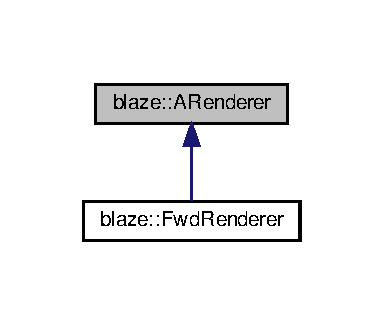
\includegraphics[width=184pt]{classblaze_1_1ARenderer__inherit__graph}
\end{center}
\end{figure}


Collaboration diagram for blaze\+:\+:A\+Renderer\+:\nopagebreak
\begin{figure}[H]
\begin{center}
\leavevmode
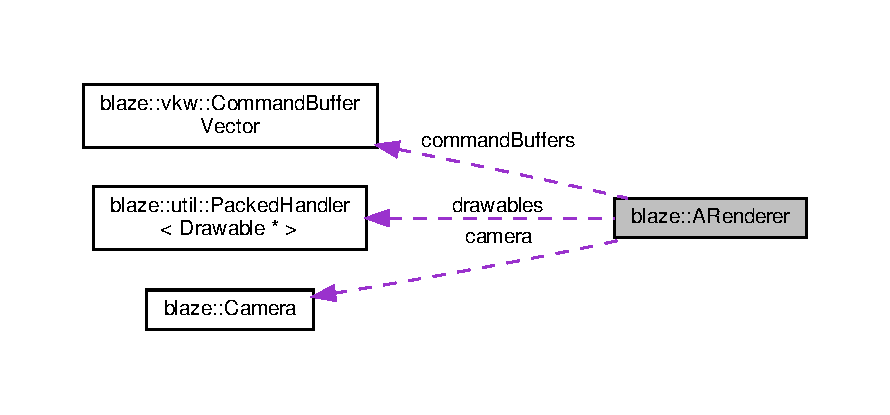
\includegraphics[width=350pt]{classblaze_1_1ARenderer__coll__graph}
\end{center}
\end{figure}
\subsection*{Public Member Functions}
\begin{DoxyCompactItemize}
\item 
\mbox{\Hypertarget{classblaze_1_1ARenderer_a50df05637f7901c6c250cac7589339b3}\label{classblaze_1_1ARenderer_a50df05637f7901c6c250cac7589339b3}} 
{\bfseries A\+Renderer} (G\+L\+F\+Wwindow $\ast$window, bool enable\+Validation\+Layers=true) noexcept
\item 
\mbox{\Hypertarget{classblaze_1_1ARenderer_a6afdc08bbc3b63db882d905da16e21d6}\label{classblaze_1_1ARenderer_a6afdc08bbc3b63db882d905da16e21d6}} 
{\bfseries A\+Renderer} (\hyperlink{classblaze_1_1ARenderer}{A\+Renderer} \&\&other)=delete
\item 
\mbox{\Hypertarget{classblaze_1_1ARenderer_a88a86e280f936a5c87869f933a753e7c}\label{classblaze_1_1ARenderer_a88a86e280f936a5c87869f933a753e7c}} 
\hyperlink{classblaze_1_1ARenderer}{A\+Renderer} \& {\bfseries operator=} (\hyperlink{classblaze_1_1ARenderer}{A\+Renderer} \&\&other)=delete
\item 
\mbox{\Hypertarget{classblaze_1_1ARenderer_a5569c604df77ac33fdb245bc71b8ed32}\label{classblaze_1_1ARenderer_a5569c604df77ac33fdb245bc71b8ed32}} 
{\bfseries A\+Renderer} (const \hyperlink{classblaze_1_1ARenderer}{A\+Renderer} \&other)=delete
\item 
\mbox{\Hypertarget{classblaze_1_1ARenderer_ab805d9247321d41fae868da36fe83d91}\label{classblaze_1_1ARenderer_ab805d9247321d41fae868da36fe83d91}} 
\hyperlink{classblaze_1_1ARenderer}{A\+Renderer} \& {\bfseries operator=} (const \hyperlink{classblaze_1_1ARenderer}{A\+Renderer} \&other)=delete
\item 
\mbox{\Hypertarget{classblaze_1_1ARenderer_acf2380c5d2277beec46cddcc6f6a1ecb}\label{classblaze_1_1ARenderer_acf2380c5d2277beec46cddcc6f6a1ecb}} 
void {\bfseries render} ()
\item 
\mbox{\Hypertarget{classblaze_1_1ARenderer_a0d1b8749a57e76e1b77500b1f0ee5156}\label{classblaze_1_1ARenderer_a0d1b8749a57e76e1b77500b1f0ee5156}} 
virtual \hyperlink{structblaze_1_1spirv_1_1SetSingleton}{spirv\+::\+Set\+Singleton} {\bfseries create\+Material\+Set} ()=0
\item 
\mbox{\Hypertarget{classblaze_1_1ARenderer_a902ff28fc355bc4d076a9bb8fde8e646}\label{classblaze_1_1ARenderer_a902ff28fc355bc4d076a9bb8fde8e646}} 
virtual void {\bfseries set\+Environment} (const \hyperlink{classblaze_1_1Bindable}{Bindable} $\ast$env)=0
\item 
\mbox{\Hypertarget{classblaze_1_1ARenderer_a1d11ebeeb512737eb6a83e41e08dd4b7}\label{classblaze_1_1ARenderer_a1d11ebeeb512737eb6a83e41e08dd4b7}} 
virtual const \hyperlink{structblaze_1_1spirv_1_1Shader}{spirv\+::\+Shader} \& {\bfseries get\+\_\+shader} () const =0
\item 
\mbox{\Hypertarget{classblaze_1_1ARenderer_ae7d0ba1357bb08846d9e1560d216f941}\label{classblaze_1_1ARenderer_ae7d0ba1357bb08846d9e1560d216f941}} 
void {\bfseries set\+\_\+camera} (\hyperlink{classblaze_1_1Camera}{Camera} $\ast$p\+\_\+camera)
\item 
\mbox{\Hypertarget{classblaze_1_1ARenderer_aac99ae31776dd569358e5c3789698eda}\label{classblaze_1_1ARenderer_aac99ae31776dd569358e5c3789698eda}} 
const \hyperlink{classblaze_1_1Context}{Context} $\ast$ {\bfseries get\+\_\+context} () const
\item 
\mbox{\Hypertarget{classblaze_1_1ARenderer_ad51e674928ead1dd0de3b47eac1016e8}\label{classblaze_1_1ARenderer_ad51e674928ead1dd0de3b47eac1016e8}} 
\hyperlink{classblaze_1_1spirv_1_1PipelineFactory}{spirv\+::\+Pipeline\+Factory} $\ast$ {\bfseries get\+\_\+pipeline\+Factory} ()
\item 
\mbox{\Hypertarget{classblaze_1_1ARenderer_a16f2a88de5037de409395d7c372a78b1}\label{classblaze_1_1ARenderer_a16f2a88de5037de409395d7c372a78b1}} 
Draw\+List\+::\+Handle {\bfseries submit} (\hyperlink{classblaze_1_1Drawable}{Drawable} $\ast$sub)
\item 
\mbox{\Hypertarget{classblaze_1_1ARenderer_a96980e0eb62b07195e3bb0e028b51da1}\label{classblaze_1_1ARenderer_a96980e0eb62b07195e3bb0e028b51da1}} 
bool {\bfseries complete} ()
\item 
\mbox{\Hypertarget{classblaze_1_1ARenderer_ae6042349671dc48ec48c73ff60934a56}\label{classblaze_1_1ARenderer_ae6042349671dc48ec48c73ff60934a56}} 
void {\bfseries wait\+Idle} ()
\end{DoxyCompactItemize}
\subsection*{Protected Types}
\begin{DoxyCompactItemize}
\item 
\mbox{\Hypertarget{classblaze_1_1ARenderer_afe4f1ac0fa4f6af7c49d0421020d7cec}\label{classblaze_1_1ARenderer_afe4f1ac0fa4f6af7c49d0421020d7cec}} 
using {\bfseries Draw\+List} = \hyperlink{classblaze_1_1util_1_1PackedHandler}{util\+::\+Packed\+Handler}$<$ \hyperlink{classblaze_1_1Drawable}{Drawable} $\ast$ $>$
\end{DoxyCompactItemize}
\subsection*{Protected Member Functions}
\begin{DoxyCompactItemize}
\item 
\mbox{\Hypertarget{classblaze_1_1ARenderer_abc172e917d52ebd9684fbfc91e83fded}\label{classblaze_1_1ARenderer_abc172e917d52ebd9684fbfc91e83fded}} 
void {\bfseries recreate\+Swapchain} ()
\item 
\mbox{\Hypertarget{classblaze_1_1ARenderer_ad9f386a77a9ce923901d9aa0f8379faa}\label{classblaze_1_1ARenderer_ad9f386a77a9ce923901d9aa0f8379faa}} 
std\+::pair$<$ uint32\+\_\+t, uint32\+\_\+t $>$ {\bfseries get\+\_\+dimensions} () const
\item 
\mbox{\Hypertarget{classblaze_1_1ARenderer_a47d147ed52d4e01b2b1e84e73bf4f383}\label{classblaze_1_1ARenderer_a47d147ed52d4e01b2b1e84e73bf4f383}} 
void {\bfseries clear\+Command\+Buffers} ()
\item 
\mbox{\Hypertarget{classblaze_1_1ARenderer_a2a157380cb98e09ca023abc79663a0b6}\label{classblaze_1_1ARenderer_a2a157380cb98e09ca023abc79663a0b6}} 
void {\bfseries rebuild\+All\+Command\+Buffers} ()
\item 
\mbox{\Hypertarget{classblaze_1_1ARenderer_ae0f6fef0b400eefa7e1403dac4ff1cfd}\label{classblaze_1_1ARenderer_ae0f6fef0b400eefa7e1403dac4ff1cfd}} 
void {\bfseries rebuild\+Command\+Buffer} (uint32\+\_\+t frame)
\item 
\mbox{\Hypertarget{classblaze_1_1ARenderer_a45d78544834276139f73316b80e18577}\label{classblaze_1_1ARenderer_a45d78544834276139f73316b80e18577}} 
virtual void {\bfseries update} (uint32\+\_\+t frame)=0
\item 
\mbox{\Hypertarget{classblaze_1_1ARenderer_a364ef6ff07211f5b3d611c230c413cea}\label{classblaze_1_1ARenderer_a364ef6ff07211f5b3d611c230c413cea}} 
virtual void {\bfseries record\+Commands} (uint32\+\_\+t frame)=0
\item 
\mbox{\Hypertarget{classblaze_1_1ARenderer_a1db2f2b5de282cb85e5344744e91a7ab}\label{classblaze_1_1ARenderer_a1db2f2b5de282cb85e5344744e91a7ab}} 
virtual void {\bfseries recreate\+Swapchain\+Dependents} ()=0
\end{DoxyCompactItemize}
\subsection*{Protected Attributes}
\begin{DoxyCompactItemize}
\item 
\mbox{\Hypertarget{classblaze_1_1ARenderer_a1d729975bd96063dfbd3821a4bc222a1}\label{classblaze_1_1ARenderer_a1d729975bd96063dfbd3821a4bc222a1}} 
uint32\+\_\+t {\bfseries max\+Frame\+In\+Flight} \{2\}
\item 
\mbox{\Hypertarget{classblaze_1_1ARenderer_a920af9542eed368dfd37523f7584a6ba}\label{classblaze_1_1ARenderer_a920af9542eed368dfd37523f7584a6ba}} 
bool {\bfseries is\+Complete} \{false\}
\item 
\mbox{\Hypertarget{classblaze_1_1ARenderer_ae3afe1ea7a452bb0ec29c210639b56b0}\label{classblaze_1_1ARenderer_ae3afe1ea7a452bb0ec29c210639b56b0}} 
bool {\bfseries window\+Resized} \{false\}
\item 
\mbox{\Hypertarget{classblaze_1_1ARenderer_a79cf50d4481bfb4a21d57fa5c4ddfc93}\label{classblaze_1_1ARenderer_a79cf50d4481bfb4a21d57fa5c4ddfc93}} 
uint32\+\_\+t {\bfseries current\+Frame} \{0\}
\item 
\mbox{\Hypertarget{classblaze_1_1ARenderer_a4ffd40adc9cabeda6612b7cdaa0f399e}\label{classblaze_1_1ARenderer_a4ffd40adc9cabeda6612b7cdaa0f399e}} 
std\+::unique\+\_\+ptr$<$ \hyperlink{classblaze_1_1Context}{Context} $>$ {\bfseries context}
\item 
\mbox{\Hypertarget{classblaze_1_1ARenderer_a0c22712edcd9d888fe0756db095d1593}\label{classblaze_1_1ARenderer_a0c22712edcd9d888fe0756db095d1593}} 
std\+::unique\+\_\+ptr$<$ \hyperlink{classblaze_1_1Swapchain}{Swapchain} $>$ {\bfseries swapchain}
\item 
\mbox{\Hypertarget{classblaze_1_1ARenderer_a20d9e0ae9052051bb130435aee323861}\label{classblaze_1_1ARenderer_a20d9e0ae9052051bb130435aee323861}} 
std\+::unique\+\_\+ptr$<$ \hyperlink{classblaze_1_1GUI}{G\+UI} $>$ {\bfseries gui}
\item 
\mbox{\Hypertarget{classblaze_1_1ARenderer_a66f91ba2792d8678a15c3ce6e64df353}\label{classblaze_1_1ARenderer_a66f91ba2792d8678a15c3ce6e64df353}} 
\hyperlink{classblaze_1_1Camera}{Camera} $\ast$ {\bfseries camera} \{nullptr\}
\item 
\mbox{\Hypertarget{classblaze_1_1ARenderer_ac7a96d61032c07c7166720a80b68c81e}\label{classblaze_1_1ARenderer_ac7a96d61032c07c7166720a80b68c81e}} 
\hyperlink{structblaze_1_1vkw_1_1CommandBufferVector}{vkw\+::\+Command\+Buffer\+Vector} {\bfseries command\+Buffers}
\item 
\mbox{\Hypertarget{classblaze_1_1ARenderer_accaa640496d736ae46f0cc0549b0b59e}\label{classblaze_1_1ARenderer_accaa640496d736ae46f0cc0549b0b59e}} 
vkw\+::\+Semaphore\+Vector {\bfseries image\+Available\+Sem}
\item 
\mbox{\Hypertarget{classblaze_1_1ARenderer_a351ea8ada814a74953b624e34d91c7a1}\label{classblaze_1_1ARenderer_a351ea8ada814a74953b624e34d91c7a1}} 
vkw\+::\+Semaphore\+Vector {\bfseries render\+Finished\+Sem}
\item 
\mbox{\Hypertarget{classblaze_1_1ARenderer_ac7a5a6d1ab20ead4d903d4867aa6c81b}\label{classblaze_1_1ARenderer_ac7a5a6d1ab20ead4d903d4867aa6c81b}} 
vkw\+::\+Fence\+Vector {\bfseries in\+Flight\+Fences}
\item 
\mbox{\Hypertarget{classblaze_1_1ARenderer_ae5ca0812615c13266803055936c6fdd0}\label{classblaze_1_1ARenderer_ae5ca0812615c13266803055936c6fdd0}} 
std\+::unique\+\_\+ptr$<$ \hyperlink{classblaze_1_1spirv_1_1PipelineFactory}{spirv\+::\+Pipeline\+Factory} $>$ {\bfseries pipeline\+Factory}
\item 
\mbox{\Hypertarget{classblaze_1_1ARenderer_a2131f0ab8880d1165fcfa9586b4a32f0}\label{classblaze_1_1ARenderer_a2131f0ab8880d1165fcfa9586b4a32f0}} 
\hyperlink{classblaze_1_1util_1_1PackedHandler}{Draw\+List} {\bfseries drawables}
\end{DoxyCompactItemize}


The documentation for this class was generated from the following files\+:\begin{DoxyCompactItemize}
\item 
Blaze/rendering/A\+Renderer.\+hpp\item 
Blaze/rendering/A\+Renderer.\+cpp\end{DoxyCompactItemize}

\hypertarget{structblaze_1_1spirv_1_1AttachmentFormat}{}\section{blaze\+:\+:spirv\+:\+:Attachment\+Format Struct Reference}
\label{structblaze_1_1spirv_1_1AttachmentFormat}\index{blaze\+::spirv\+::\+Attachment\+Format@{blaze\+::spirv\+::\+Attachment\+Format}}
\subsection*{Public Member Functions}
\begin{DoxyCompactItemize}
\item 
\mbox{\Hypertarget{structblaze_1_1spirv_1_1AttachmentFormat_ab10e95ec7d36ef9d1050b52012f096a4}\label{structblaze_1_1spirv_1_1AttachmentFormat_ab10e95ec7d36ef9d1050b52012f096a4}} 
bool {\bfseries operator!=} (const \hyperlink{structblaze_1_1spirv_1_1AttachmentFormat}{Attachment\+Format} \&other) const
\item 
\mbox{\Hypertarget{structblaze_1_1spirv_1_1AttachmentFormat_aa6a382474e14a3472b43fbf8c0c24a51}\label{structblaze_1_1spirv_1_1AttachmentFormat_aa6a382474e14a3472b43fbf8c0c24a51}} 
bool {\bfseries operator$<$} (const \hyperlink{structblaze_1_1spirv_1_1AttachmentFormat}{Attachment\+Format} \&other) const
\end{DoxyCompactItemize}
\subsection*{Public Attributes}
\begin{DoxyCompactItemize}
\item 
\mbox{\Hypertarget{structblaze_1_1spirv_1_1AttachmentFormat_a417342f2fdf69c9cfab2833ab7df71d2}\label{structblaze_1_1spirv_1_1AttachmentFormat_a417342f2fdf69c9cfab2833ab7df71d2}} 
Vk\+Image\+Usage\+Flags {\bfseries usage}
\item 
\mbox{\Hypertarget{structblaze_1_1spirv_1_1AttachmentFormat_a92ed50ec8aff210e94205a0754924654}\label{structblaze_1_1spirv_1_1AttachmentFormat_a92ed50ec8aff210e94205a0754924654}} 
Vk\+Format {\bfseries format}
\item 
\mbox{\Hypertarget{structblaze_1_1spirv_1_1AttachmentFormat_adff102a8e3fc33345a1a25daf05288a1}\label{structblaze_1_1spirv_1_1AttachmentFormat_adff102a8e3fc33345a1a25daf05288a1}} 
Vk\+Sample\+Count\+Flag\+Bits {\bfseries sample\+Count}
\end{DoxyCompactItemize}


The documentation for this struct was generated from the following file\+:\begin{DoxyCompactItemize}
\item 
Blaze/spirv/Pipeline\+Factory.\+hpp\end{DoxyCompactItemize}

\hypertarget{classblaze_1_1util_1_1AutoTimer}{}\section{blaze\+:\+:util\+:\+:Auto\+Timer Class Reference}
\label{classblaze_1_1util_1_1AutoTimer}\index{blaze\+::util\+::\+Auto\+Timer@{blaze\+::util\+::\+Auto\+Timer}}
\subsection*{Public Member Functions}
\begin{DoxyCompactItemize}
\item 
\mbox{\Hypertarget{classblaze_1_1util_1_1AutoTimer_ae8c4b739eac9a9ea39c1d6a092976967}\label{classblaze_1_1util_1_1AutoTimer_ae8c4b739eac9a9ea39c1d6a092976967}} 
{\bfseries Auto\+Timer} (const std\+::string \&msg)
\end{DoxyCompactItemize}


The documentation for this class was generated from the following file\+:\begin{DoxyCompactItemize}
\item 
Blaze/util/Debug\+Timer.\+hpp\end{DoxyCompactItemize}

\hypertarget{structblaze_1_1vkw_1_1base_1_1BaseCollection}{}\section{blaze\+:\+:vkw\+:\+:base\+:\+:Base\+Collection$<$ T\+Handle $>$ Struct Template Reference}
\label{structblaze_1_1vkw_1_1base_1_1BaseCollection}\index{blaze\+::vkw\+::base\+::\+Base\+Collection$<$ T\+Handle $>$@{blaze\+::vkw\+::base\+::\+Base\+Collection$<$ T\+Handle $>$}}


The basic collection wrapper for uniformity.  




{\ttfamily \#include $<$Vk\+Wrap\+Base.\+hpp$>$}

\subsection*{Public Member Functions}
\begin{DoxyCompactItemize}
\item 
\mbox{\Hypertarget{structblaze_1_1vkw_1_1base_1_1BaseCollection_ab41cf18a4e885e7c6791092ff8a1226a}\label{structblaze_1_1vkw_1_1base_1_1BaseCollection_ab41cf18a4e885e7c6791092ff8a1226a}} 
\hyperlink{structblaze_1_1vkw_1_1base_1_1BaseCollection_ab41cf18a4e885e7c6791092ff8a1226a}{Base\+Collection} () noexcept
\begin{DoxyCompactList}\small\item\em Default Constructor. \end{DoxyCompactList}\item 
\hyperlink{structblaze_1_1vkw_1_1base_1_1BaseCollection_a615d6c0aa6602f2f5678fed9e6ad1559}{Base\+Collection} (std\+::vector$<$ T\+Handle $>$ \&\&handles) noexcept
\begin{DoxyCompactList}\small\item\em Main constructor. \end{DoxyCompactList}\item 
\mbox{\Hypertarget{structblaze_1_1vkw_1_1base_1_1BaseCollection_a576b6d6312816939600f11480c1c0e63}\label{structblaze_1_1vkw_1_1base_1_1BaseCollection_a576b6d6312816939600f11480c1c0e63}} 
const std\+::vector$<$ T\+Handle $>$ \& \hyperlink{structblaze_1_1vkw_1_1base_1_1BaseCollection_a576b6d6312816939600f11480c1c0e63}{get} () const
\begin{DoxyCompactList}\small\item\em Gets the vector of handles. \end{DoxyCompactList}\item 
\mbox{\Hypertarget{structblaze_1_1vkw_1_1base_1_1BaseCollection_a733d88e7838b830b7f80252698f9fe5e}\label{structblaze_1_1vkw_1_1base_1_1BaseCollection_a733d88e7838b830b7f80252698f9fe5e}} 
const T\+Handle \& \hyperlink{structblaze_1_1vkw_1_1base_1_1BaseCollection_a733d88e7838b830b7f80252698f9fe5e}{operator\mbox{[}$\,$\mbox{]}} (uint32\+\_\+t idx) const
\begin{DoxyCompactList}\small\item\em Indexing operator that exposes the handle. \end{DoxyCompactList}\item 
\mbox{\Hypertarget{structblaze_1_1vkw_1_1base_1_1BaseCollection_a850c9787154a4915fdad3714d6567838}\label{structblaze_1_1vkw_1_1base_1_1BaseCollection_a850c9787154a4915fdad3714d6567838}} 
uint32\+\_\+t \hyperlink{structblaze_1_1vkw_1_1base_1_1BaseCollection_a850c9787154a4915fdad3714d6567838}{size} () const
\begin{DoxyCompactList}\small\item\em Returns the number of handles owned. \end{DoxyCompactList}\item 
bool \hyperlink{structblaze_1_1vkw_1_1base_1_1BaseCollection_a16ba74b297d8f157b47fc1335e79fb88}{valid} () const
\begin{DoxyCompactList}\small\item\em Checks validity. \end{DoxyCompactList}\item 
\hyperlink{structblaze_1_1vkw_1_1base_1_1BaseCollection_a17dacc1364ad11abd1c3589980e8f689}{$\sim$\+Base\+Collection} ()
\begin{DoxyCompactList}\small\item\em Destructor. \end{DoxyCompactList}\end{DoxyCompactItemize}
\begin{Indent}\textbf{ Move Constructors.}\par
{\em Copy Deleted. }\begin{DoxyCompactItemize}
\item 
\mbox{\Hypertarget{structblaze_1_1vkw_1_1base_1_1BaseCollection_a9276c08c0fe56136b2847e8e09c8088f}\label{structblaze_1_1vkw_1_1base_1_1BaseCollection_a9276c08c0fe56136b2847e8e09c8088f}} 
{\bfseries Base\+Collection} (const \hyperlink{structblaze_1_1vkw_1_1base_1_1BaseCollection}{Base\+Collection} \&other)=delete
\item 
\mbox{\Hypertarget{structblaze_1_1vkw_1_1base_1_1BaseCollection_a8d9d207776dc00baea4196a0edbb6379}\label{structblaze_1_1vkw_1_1base_1_1BaseCollection_a8d9d207776dc00baea4196a0edbb6379}} 
\hyperlink{structblaze_1_1vkw_1_1base_1_1BaseCollection}{Base\+Collection} \& {\bfseries operator=} (const \hyperlink{structblaze_1_1vkw_1_1base_1_1BaseCollection}{Base\+Collection} \&other)=delete
\item 
\mbox{\Hypertarget{structblaze_1_1vkw_1_1base_1_1BaseCollection_a182b96be903548e6ca98f8a2e038afdc}\label{structblaze_1_1vkw_1_1base_1_1BaseCollection_a182b96be903548e6ca98f8a2e038afdc}} 
{\bfseries Base\+Collection} (\hyperlink{structblaze_1_1vkw_1_1base_1_1BaseCollection}{Base\+Collection} \&\&other) noexcept
\item 
\mbox{\Hypertarget{structblaze_1_1vkw_1_1base_1_1BaseCollection_a05e4a5f383861ea15aea85c78d4a8312}\label{structblaze_1_1vkw_1_1base_1_1BaseCollection_a05e4a5f383861ea15aea85c78d4a8312}} 
\hyperlink{structblaze_1_1vkw_1_1base_1_1BaseCollection}{Base\+Collection} \& {\bfseries operator=} (\hyperlink{structblaze_1_1vkw_1_1base_1_1BaseCollection}{Base\+Collection} \&\&other) noexcept
\end{DoxyCompactItemize}
\end{Indent}
\subsection*{Public Attributes}
\begin{DoxyCompactItemize}
\item 
\mbox{\Hypertarget{structblaze_1_1vkw_1_1base_1_1BaseCollection_a1ad439023007af5c6e811d1ce98d5191}\label{structblaze_1_1vkw_1_1base_1_1BaseCollection_a1ad439023007af5c6e811d1ce98d5191}} 
std\+::vector$<$ T\+Handle $>$ {\bfseries handles}
\end{DoxyCompactItemize}


\subsection{Detailed Description}
\subsubsection*{template$<$typename T\+Handle$>$\newline
struct blaze\+::vkw\+::base\+::\+Base\+Collection$<$ T\+Handle $>$}

The basic collection wrapper for uniformity. 

\hyperlink{structblaze_1_1vkw_1_1base_1_1BaseCollection}{Base\+Collection} is only used for generating unmanaged wrapper around a collection of handles.


\begin{DoxyTemplParams}{Template Parameters}
{\em T\+Handle} & The type of handle to own. \\
\hline
\end{DoxyTemplParams}


\subsection{Constructor \& Destructor Documentation}
\mbox{\Hypertarget{structblaze_1_1vkw_1_1base_1_1BaseCollection_a615d6c0aa6602f2f5678fed9e6ad1559}\label{structblaze_1_1vkw_1_1base_1_1BaseCollection_a615d6c0aa6602f2f5678fed9e6ad1559}} 
\index{blaze\+::vkw\+::base\+::\+Base\+Collection@{blaze\+::vkw\+::base\+::\+Base\+Collection}!Base\+Collection@{Base\+Collection}}
\index{Base\+Collection@{Base\+Collection}!blaze\+::vkw\+::base\+::\+Base\+Collection@{blaze\+::vkw\+::base\+::\+Base\+Collection}}
\subsubsection{\texorpdfstring{Base\+Collection()}{BaseCollection()}}
{\footnotesize\ttfamily template$<$typename T\+Handle $>$ \\
\hyperlink{structblaze_1_1vkw_1_1base_1_1BaseCollection}{blaze\+::vkw\+::base\+::\+Base\+Collection}$<$ T\+Handle $>$\+::\hyperlink{structblaze_1_1vkw_1_1base_1_1BaseCollection}{Base\+Collection} (\begin{DoxyParamCaption}\item[{std\+::vector$<$ T\+Handle $>$ \&\&}]{handles }\end{DoxyParamCaption})\hspace{0.3cm}{\ttfamily [inline]}, {\ttfamily [explicit]}, {\ttfamily [noexcept]}}



Main constructor. 

The handles are considered as owned by the wrapper. The wrapper is explicit in order to denote that, and the handles have to be moved in.


\begin{DoxyParams}{Parameters}
{\em handles} & The vector of Vulkan handles to own. \\
\hline
\end{DoxyParams}
\mbox{\Hypertarget{structblaze_1_1vkw_1_1base_1_1BaseCollection_a17dacc1364ad11abd1c3589980e8f689}\label{structblaze_1_1vkw_1_1base_1_1BaseCollection_a17dacc1364ad11abd1c3589980e8f689}} 
\index{blaze\+::vkw\+::base\+::\+Base\+Collection@{blaze\+::vkw\+::base\+::\+Base\+Collection}!````~Base\+Collection@{$\sim$\+Base\+Collection}}
\index{````~Base\+Collection@{$\sim$\+Base\+Collection}!blaze\+::vkw\+::base\+::\+Base\+Collection@{blaze\+::vkw\+::base\+::\+Base\+Collection}}
\subsubsection{\texorpdfstring{$\sim$\+Base\+Collection()}{~BaseCollection()}}
{\footnotesize\ttfamily template$<$typename T\+Handle $>$ \\
\hyperlink{structblaze_1_1vkw_1_1base_1_1BaseCollection}{blaze\+::vkw\+::base\+::\+Base\+Collection}$<$ T\+Handle $>$\+::$\sim$\hyperlink{structblaze_1_1vkw_1_1base_1_1BaseCollection}{Base\+Collection} (\begin{DoxyParamCaption}{ }\end{DoxyParamCaption})\hspace{0.3cm}{\ttfamily [inline]}}



Destructor. 

Clears the vector of handles owned. 

\subsection{Member Function Documentation}
\mbox{\Hypertarget{structblaze_1_1vkw_1_1base_1_1BaseCollection_a16ba74b297d8f157b47fc1335e79fb88}\label{structblaze_1_1vkw_1_1base_1_1BaseCollection_a16ba74b297d8f157b47fc1335e79fb88}} 
\index{blaze\+::vkw\+::base\+::\+Base\+Collection@{blaze\+::vkw\+::base\+::\+Base\+Collection}!valid@{valid}}
\index{valid@{valid}!blaze\+::vkw\+::base\+::\+Base\+Collection@{blaze\+::vkw\+::base\+::\+Base\+Collection}}
\subsubsection{\texorpdfstring{valid()}{valid()}}
{\footnotesize\ttfamily template$<$typename T\+Handle $>$ \\
bool \hyperlink{structblaze_1_1vkw_1_1base_1_1BaseCollection}{blaze\+::vkw\+::base\+::\+Base\+Collection}$<$ T\+Handle $>$\+::valid (\begin{DoxyParamCaption}{ }\end{DoxyParamCaption}) const\hspace{0.3cm}{\ttfamily [inline]}}



Checks validity. 

Validity is defined as whether the handles are empty -\/ since that is the default initialization. 

The documentation for this struct was generated from the following file\+:\begin{DoxyCompactItemize}
\item 
Blaze/vkwrap/Vk\+Wrap\+Base.\+hpp\end{DoxyCompactItemize}

\hypertarget{classblaze_1_1BaseUBO}{}\section{blaze\+:\+:Base\+U\+BO Class Reference}
\label{classblaze_1_1BaseUBO}\index{blaze\+::\+Base\+U\+BO@{blaze\+::\+Base\+U\+BO}}


The base class for all U\+B\+Os.  




{\ttfamily \#include $<$Uniform\+Buffer.\+hpp$>$}



Inheritance diagram for blaze\+:\+:Base\+U\+BO\+:\nopagebreak
\begin{figure}[H]
\begin{center}
\leavevmode
\includegraphics[width=312pt]{classblaze_1_1BaseUBO__inherit__graph}
\end{center}
\end{figure}
\subsection*{Public Member Functions}
\begin{DoxyCompactItemize}
\item 
\mbox{\Hypertarget{classblaze_1_1BaseUBO_a09e8e765c69b703b4479b919ff5862de}\label{classblaze_1_1BaseUBO_a09e8e765c69b703b4479b919ff5862de}} 
\hyperlink{classblaze_1_1BaseUBO_a09e8e765c69b703b4479b919ff5862de}{Base\+U\+BO} () noexcept
\begin{DoxyCompactList}\small\item\em Default Constructor. \end{DoxyCompactList}\item 
\hyperlink{classblaze_1_1BaseUBO_abc55449d131e9bb970f057ee129d3728}{Base\+U\+BO} (const \hyperlink{classblaze_1_1Context}{Context} $\ast$context, size\+\_\+t size) noexcept
\begin{DoxyCompactList}\small\item\em Main Constructor. \end{DoxyCompactList}\item 
\mbox{\Hypertarget{classblaze_1_1BaseUBO_af9d9c0c2ddf95090773412488c14fa9e}\label{classblaze_1_1BaseUBO_af9d9c0c2ddf95090773412488c14fa9e}} 
Vk\+Descriptor\+Buffer\+Info \hyperlink{classblaze_1_1BaseUBO_af9d9c0c2ddf95090773412488c14fa9e}{get\+\_\+descriptor\+Info} () const
\begin{DoxyCompactList}\small\item\em Creates a new Vk\+Descriptor\+Buffer\+Info for the \hyperlink{classblaze_1_1UBO}{U\+BO}. \end{DoxyCompactList}\item 
\mbox{\Hypertarget{classblaze_1_1BaseUBO_a4a07203396a3ac3b29eca729149de8ca}\label{classblaze_1_1BaseUBO_a4a07203396a3ac3b29eca729149de8ca}} 
virtual \hyperlink{classblaze_1_1BaseUBO_a4a07203396a3ac3b29eca729149de8ca}{$\sim$\+Base\+U\+BO} ()
\begin{DoxyCompactList}\small\item\em Destructor. \end{DoxyCompactList}\end{DoxyCompactItemize}
\begin{Indent}\textbf{ Move Constructors.}\par
{\em Move only, copy deleted. }\begin{DoxyCompactItemize}
\item 
\mbox{\Hypertarget{classblaze_1_1BaseUBO_aa4e8c0e3f7e7fd07dc58683813e5d033}\label{classblaze_1_1BaseUBO_aa4e8c0e3f7e7fd07dc58683813e5d033}} 
{\bfseries Base\+U\+BO} (\hyperlink{classblaze_1_1BaseUBO}{Base\+U\+BO} \&\&other) noexcept
\item 
\mbox{\Hypertarget{classblaze_1_1BaseUBO_a6f81e5b988d6693ff9ac377b7e2d11ea}\label{classblaze_1_1BaseUBO_a6f81e5b988d6693ff9ac377b7e2d11ea}} 
\hyperlink{classblaze_1_1BaseUBO}{Base\+U\+BO} \& {\bfseries operator=} (\hyperlink{classblaze_1_1BaseUBO}{Base\+U\+BO} \&\&other) noexcept
\item 
\mbox{\Hypertarget{classblaze_1_1BaseUBO_abc3f978bfb601096b6d0014de995ee42}\label{classblaze_1_1BaseUBO_abc3f978bfb601096b6d0014de995ee42}} 
{\bfseries Base\+U\+BO} (const \hyperlink{classblaze_1_1BaseUBO}{Base\+U\+BO} \&other)=delete
\item 
\mbox{\Hypertarget{classblaze_1_1BaseUBO_af29582dab41fdc03211a425ab2c09427}\label{classblaze_1_1BaseUBO_af29582dab41fdc03211a425ab2c09427}} 
\hyperlink{classblaze_1_1BaseUBO}{Base\+U\+BO} \& {\bfseries operator=} (const \hyperlink{classblaze_1_1BaseUBO}{Base\+U\+BO} \&other)=delete
\end{DoxyCompactItemize}
\end{Indent}
\subsection*{Protected Member Functions}
\begin{DoxyCompactItemize}
\item 
void \hyperlink{classblaze_1_1BaseUBO_a76859304045ec034ea2cffe68ea1db65}{write\+Data} (const void $\ast$data, size\+\_\+t size)
\begin{DoxyCompactList}\small\item\em Writes data to the buffer. \end{DoxyCompactList}\end{DoxyCompactItemize}
\subsection*{Protected Attributes}
\begin{DoxyCompactItemize}
\item 
\mbox{\Hypertarget{classblaze_1_1BaseUBO_a1a8439adc16530d7630ba918251f3f74}\label{classblaze_1_1BaseUBO_a1a8439adc16530d7630ba918251f3f74}} 
Vk\+Buffer {\bfseries buffer} \{V\+K\+\_\+\+N\+U\+L\+L\+\_\+\+H\+A\+N\+D\+LE\}
\item 
\mbox{\Hypertarget{classblaze_1_1BaseUBO_a14f3711ae432dc6d3dcfc9cc26547152}\label{classblaze_1_1BaseUBO_a14f3711ae432dc6d3dcfc9cc26547152}} 
Vma\+Allocation {\bfseries allocation} \{V\+K\+\_\+\+N\+U\+L\+L\+\_\+\+H\+A\+N\+D\+LE\}
\item 
\mbox{\Hypertarget{classblaze_1_1BaseUBO_a880896ef02c52bb2d7e4ddd566cd9cab}\label{classblaze_1_1BaseUBO_a880896ef02c52bb2d7e4ddd566cd9cab}} 
Vma\+Allocator {\bfseries allocator} \{V\+K\+\_\+\+N\+U\+L\+L\+\_\+\+H\+A\+N\+D\+LE\}
\item 
\mbox{\Hypertarget{classblaze_1_1BaseUBO_a8e0a6327bf61125c790d5fc036fcef62}\label{classblaze_1_1BaseUBO_a8e0a6327bf61125c790d5fc036fcef62}} 
size\+\_\+t {\bfseries size} \{0\}
\end{DoxyCompactItemize}


\subsection{Detailed Description}
The base class for all U\+B\+Os. 

The type independent size dependent generic class to implement a buffer for uniforms. Mostly not to be used directly, but extended by a type safe derived class. 

\subsection{Constructor \& Destructor Documentation}
\mbox{\Hypertarget{classblaze_1_1BaseUBO_abc55449d131e9bb970f057ee129d3728}\label{classblaze_1_1BaseUBO_abc55449d131e9bb970f057ee129d3728}} 
\index{blaze\+::\+Base\+U\+BO@{blaze\+::\+Base\+U\+BO}!Base\+U\+BO@{Base\+U\+BO}}
\index{Base\+U\+BO@{Base\+U\+BO}!blaze\+::\+Base\+U\+BO@{blaze\+::\+Base\+U\+BO}}
\subsubsection{\texorpdfstring{Base\+U\+B\+O()}{BaseUBO()}}
{\footnotesize\ttfamily blaze\+::\+Base\+U\+B\+O\+::\+Base\+U\+BO (\begin{DoxyParamCaption}\item[{const \hyperlink{classblaze_1_1Context}{Context} $\ast$}]{context,  }\item[{size\+\_\+t}]{size }\end{DoxyParamCaption})\hspace{0.3cm}{\ttfamily [noexcept]}}



Main Constructor. 


\begin{DoxyParams}{Parameters}
{\em context} & Pointer to the \hyperlink{classblaze_1_1Context}{Context} in use. \\
\hline
{\em size} & The size of the actual buffer to allocate. \\
\hline
\end{DoxyParams}


\subsection{Member Function Documentation}
\mbox{\Hypertarget{classblaze_1_1BaseUBO_a76859304045ec034ea2cffe68ea1db65}\label{classblaze_1_1BaseUBO_a76859304045ec034ea2cffe68ea1db65}} 
\index{blaze\+::\+Base\+U\+BO@{blaze\+::\+Base\+U\+BO}!write\+Data@{write\+Data}}
\index{write\+Data@{write\+Data}!blaze\+::\+Base\+U\+BO@{blaze\+::\+Base\+U\+BO}}
\subsubsection{\texorpdfstring{write\+Data()}{writeData()}}
{\footnotesize\ttfamily void blaze\+::\+Base\+U\+B\+O\+::write\+Data (\begin{DoxyParamCaption}\item[{const void $\ast$}]{data,  }\item[{size\+\_\+t}]{size }\end{DoxyParamCaption})\hspace{0.3cm}{\ttfamily [protected]}}



Writes data to the buffer. 


\begin{DoxyParams}{Parameters}
{\em data} & The pointer to the data to write into buffer. \\
\hline
{\em size} & The size of the data to write into the buffer. \\
\hline
\end{DoxyParams}


The documentation for this class was generated from the following files\+:\begin{DoxyCompactItemize}
\item 
Blaze/core/Uniform\+Buffer.\+hpp\item 
Blaze/core/Uniform\+Buffer.\+cpp\end{DoxyCompactItemize}

\hypertarget{classblaze_1_1BaseVBO}{}\section{blaze\+:\+:Base\+V\+BO Class Reference}
\label{classblaze_1_1BaseVBO}\index{blaze\+::\+Base\+V\+BO@{blaze\+::\+Base\+V\+BO}}


Inheritance diagram for blaze\+:\+:Base\+V\+BO\+:\nopagebreak
\begin{figure}[H]
\begin{center}
\leavevmode
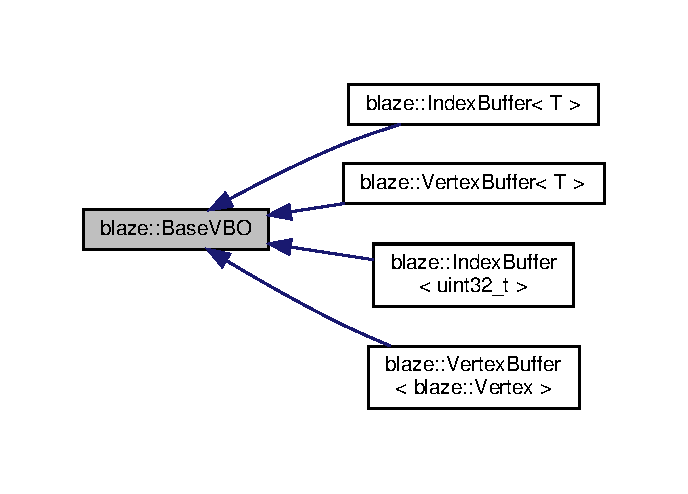
\includegraphics[width=330pt]{classblaze_1_1BaseVBO__inherit__graph}
\end{center}
\end{figure}
\subsection*{Public Types}
\begin{DoxyCompactItemize}
\item 
\mbox{\Hypertarget{classblaze_1_1BaseVBO_a0a207a857251b73334a9ee843b9c8da8}\label{classblaze_1_1BaseVBO_a0a207a857251b73334a9ee843b9c8da8}} 
enum {\bfseries Usage} \{ {\bfseries Vertex\+Buffer} = V\+K\+\_\+\+B\+U\+F\+F\+E\+R\+\_\+\+U\+S\+A\+G\+E\+\_\+\+V\+E\+R\+T\+E\+X\+\_\+\+B\+U\+F\+F\+E\+R\+\_\+\+B\+IT, 
{\bfseries Index\+Buffer} = V\+K\+\_\+\+B\+U\+F\+F\+E\+R\+\_\+\+U\+S\+A\+G\+E\+\_\+\+I\+N\+D\+E\+X\+\_\+\+B\+U\+F\+F\+E\+R\+\_\+\+B\+IT
 \}
\end{DoxyCompactItemize}
\subsection*{Public Member Functions}
\begin{DoxyCompactItemize}
\item 
\mbox{\Hypertarget{classblaze_1_1BaseVBO_a5eeef0c7e85c61eb41851047f8f98073}\label{classblaze_1_1BaseVBO_a5eeef0c7e85c61eb41851047f8f98073}} 
{\bfseries Base\+V\+BO} (const \hyperlink{classblaze_1_1Context}{Context} $\ast$context, Usage usage, const void $\ast$data, uint32\+\_\+t count, size\+\_\+t size) noexcept
\item 
\mbox{\Hypertarget{classblaze_1_1BaseVBO_a53edcf9bfcedf7f7b26d6d182f6f4f7e}\label{classblaze_1_1BaseVBO_a53edcf9bfcedf7f7b26d6d182f6f4f7e}} 
{\bfseries Base\+V\+BO} (\hyperlink{classblaze_1_1BaseVBO}{Base\+V\+BO} \&\&other) noexcept
\item 
\mbox{\Hypertarget{classblaze_1_1BaseVBO_a91d5d339c3ef4e617a9fdf1dc9ebcb19}\label{classblaze_1_1BaseVBO_a91d5d339c3ef4e617a9fdf1dc9ebcb19}} 
\hyperlink{classblaze_1_1BaseVBO}{Base\+V\+BO} \& {\bfseries operator=} (\hyperlink{classblaze_1_1BaseVBO}{Base\+V\+BO} \&\&other) noexcept
\item 
\mbox{\Hypertarget{classblaze_1_1BaseVBO_a502615b8e2aee286c9423fb44860010d}\label{classblaze_1_1BaseVBO_a502615b8e2aee286c9423fb44860010d}} 
{\bfseries Base\+V\+BO} (const \hyperlink{classblaze_1_1BaseVBO}{Base\+V\+BO} \&other)=delete
\item 
\mbox{\Hypertarget{classblaze_1_1BaseVBO_ad33b69a6e7fe316547deb97561982d29}\label{classblaze_1_1BaseVBO_ad33b69a6e7fe316547deb97561982d29}} 
\hyperlink{classblaze_1_1BaseVBO}{Base\+V\+BO} \& {\bfseries operator=} (const \hyperlink{classblaze_1_1BaseVBO}{Base\+V\+BO} \&other)=delete
\item 
\mbox{\Hypertarget{classblaze_1_1BaseVBO_aebb08170aeb719ee90ea53cab50b5a9d}\label{classblaze_1_1BaseVBO_aebb08170aeb719ee90ea53cab50b5a9d}} 
const Vk\+Buffer \& {\bfseries get\+\_\+buffer} () const
\item 
\mbox{\Hypertarget{classblaze_1_1BaseVBO_ad974bf5e5c5936770eecbaf9dd8e3c44}\label{classblaze_1_1BaseVBO_ad974bf5e5c5936770eecbaf9dd8e3c44}} 
const uint32\+\_\+t \& {\bfseries get\+\_\+count} () const
\end{DoxyCompactItemize}
\subsection*{Protected Attributes}
\begin{DoxyCompactItemize}
\item 
\mbox{\Hypertarget{classblaze_1_1BaseVBO_a3cbf6177475e40b7d0bf2bc59e3eb43a}\label{classblaze_1_1BaseVBO_a3cbf6177475e40b7d0bf2bc59e3eb43a}} 
Vk\+Buffer {\bfseries buffer} \{V\+K\+\_\+\+N\+U\+L\+L\+\_\+\+H\+A\+N\+D\+LE\}
\item 
\mbox{\Hypertarget{classblaze_1_1BaseVBO_abf5e6d6f805e6394d2e0904860baba71}\label{classblaze_1_1BaseVBO_abf5e6d6f805e6394d2e0904860baba71}} 
Vma\+Allocation {\bfseries allocation} \{V\+K\+\_\+\+N\+U\+L\+L\+\_\+\+H\+A\+N\+D\+LE\}
\item 
\mbox{\Hypertarget{classblaze_1_1BaseVBO_a37f949fdad807b65931264089540c005}\label{classblaze_1_1BaseVBO_a37f949fdad807b65931264089540c005}} 
Vma\+Allocator {\bfseries allocator} \{V\+K\+\_\+\+N\+U\+L\+L\+\_\+\+H\+A\+N\+D\+LE\}
\item 
\mbox{\Hypertarget{classblaze_1_1BaseVBO_aff756843a4b3edeea281d57cf6d148ce}\label{classblaze_1_1BaseVBO_aff756843a4b3edeea281d57cf6d148ce}} 
uint32\+\_\+t {\bfseries count} \{0\}
\item 
\mbox{\Hypertarget{classblaze_1_1BaseVBO_a670e4e4446c2286fac4b922ddb5c84f3}\label{classblaze_1_1BaseVBO_a670e4e4446c2286fac4b922ddb5c84f3}} 
size\+\_\+t {\bfseries size} \{0\}
\end{DoxyCompactItemize}


The documentation for this class was generated from the following files\+:\begin{DoxyCompactItemize}
\item 
Blaze/core/Vertex\+Buffer.\+hpp\item 
Blaze/core/Vertex\+Buffer.\+cpp\end{DoxyCompactItemize}

\hypertarget{structblaze_1_1vkw_1_1base_1_1BaseWrapper}{}\section{blaze\+:\+:vkw\+:\+:base\+:\+:Base\+Wrapper$<$ T\+Handle $>$ Struct Template Reference}
\label{structblaze_1_1vkw_1_1base_1_1BaseWrapper}\index{blaze\+::vkw\+::base\+::\+Base\+Wrapper$<$ T\+Handle $>$@{blaze\+::vkw\+::base\+::\+Base\+Wrapper$<$ T\+Handle $>$}}


The basic wrapper for uniformity.  




{\ttfamily \#include $<$Vk\+Wrap\+Base.\+hpp$>$}

\subsection*{Public Member Functions}
\begin{DoxyCompactItemize}
\item 
\mbox{\Hypertarget{structblaze_1_1vkw_1_1base_1_1BaseWrapper_a87d61fbfd8fa3fdfd8aad1a621e6a63a}\label{structblaze_1_1vkw_1_1base_1_1BaseWrapper_a87d61fbfd8fa3fdfd8aad1a621e6a63a}} 
\hyperlink{structblaze_1_1vkw_1_1base_1_1BaseWrapper_a87d61fbfd8fa3fdfd8aad1a621e6a63a}{Base\+Wrapper} () noexcept
\begin{DoxyCompactList}\small\item\em Default Constructor. \end{DoxyCompactList}\item 
\hyperlink{structblaze_1_1vkw_1_1base_1_1BaseWrapper_a5569991b2ff88d2a758dcc7d93141c96}{Base\+Wrapper} (T\+Handle handle) noexcept
\begin{DoxyCompactList}\small\item\em Main constructor. \end{DoxyCompactList}\item 
\mbox{\Hypertarget{structblaze_1_1vkw_1_1base_1_1BaseWrapper_afe04eafe1e8c18c911a648d229e4cb10}\label{structblaze_1_1vkw_1_1base_1_1BaseWrapper_afe04eafe1e8c18c911a648d229e4cb10}} 
const T\+Handle \& \hyperlink{structblaze_1_1vkw_1_1base_1_1BaseWrapper_afe04eafe1e8c18c911a648d229e4cb10}{get} () const
\begin{DoxyCompactList}\small\item\em Getter for the handle. \end{DoxyCompactList}\item 
bool \hyperlink{structblaze_1_1vkw_1_1base_1_1BaseWrapper_aa6499ac388955fe4a6a6b729f4a48ca8}{valid} () const
\begin{DoxyCompactList}\small\item\em Checks if the handle is non-\/null. \end{DoxyCompactList}\item 
\mbox{\Hypertarget{structblaze_1_1vkw_1_1base_1_1BaseWrapper_a469f239211552a5befc6bb243ded472a}\label{structblaze_1_1vkw_1_1base_1_1BaseWrapper_a469f239211552a5befc6bb243ded472a}} 
\hyperlink{structblaze_1_1vkw_1_1base_1_1BaseWrapper_a469f239211552a5befc6bb243ded472a}{$\sim$\+Base\+Wrapper} ()
\begin{DoxyCompactList}\small\item\em Destructor. \end{DoxyCompactList}\end{DoxyCompactItemize}
\begin{Indent}\textbf{ Move Constructors.}\par
{\em Coopy Deleted. }\begin{DoxyCompactItemize}
\item 
\mbox{\Hypertarget{structblaze_1_1vkw_1_1base_1_1BaseWrapper_ac64b4743de1a01d75e26886c3a8d9d43}\label{structblaze_1_1vkw_1_1base_1_1BaseWrapper_ac64b4743de1a01d75e26886c3a8d9d43}} 
{\bfseries Base\+Wrapper} (const \hyperlink{structblaze_1_1vkw_1_1base_1_1BaseWrapper}{Base\+Wrapper} \&other)=delete
\item 
\mbox{\Hypertarget{structblaze_1_1vkw_1_1base_1_1BaseWrapper_af33a63b889c8a60a4eb811bee0799ea4}\label{structblaze_1_1vkw_1_1base_1_1BaseWrapper_af33a63b889c8a60a4eb811bee0799ea4}} 
\hyperlink{structblaze_1_1vkw_1_1base_1_1BaseWrapper}{Base\+Wrapper} \& {\bfseries operator=} (const \hyperlink{structblaze_1_1vkw_1_1base_1_1BaseWrapper}{Base\+Wrapper} \&other)=delete
\item 
\mbox{\Hypertarget{structblaze_1_1vkw_1_1base_1_1BaseWrapper_a0ad98e80f12d97cf35b26f2b38553b06}\label{structblaze_1_1vkw_1_1base_1_1BaseWrapper_a0ad98e80f12d97cf35b26f2b38553b06}} 
{\bfseries Base\+Wrapper} (\hyperlink{structblaze_1_1vkw_1_1base_1_1BaseWrapper}{Base\+Wrapper} \&\&other) noexcept
\item 
\mbox{\Hypertarget{structblaze_1_1vkw_1_1base_1_1BaseWrapper_a16f1d424504044c33d699aac5ea5b9e5}\label{structblaze_1_1vkw_1_1base_1_1BaseWrapper_a16f1d424504044c33d699aac5ea5b9e5}} 
\hyperlink{structblaze_1_1vkw_1_1base_1_1BaseWrapper}{Base\+Wrapper} \& {\bfseries operator=} (\hyperlink{structblaze_1_1vkw_1_1base_1_1BaseWrapper}{Base\+Wrapper} \&\&other) noexcept
\end{DoxyCompactItemize}
\end{Indent}
\subsection*{Public Attributes}
\begin{DoxyCompactItemize}
\item 
\mbox{\Hypertarget{structblaze_1_1vkw_1_1base_1_1BaseWrapper_aa9bd63fd9b4829070702b41e1d3559b4}\label{structblaze_1_1vkw_1_1base_1_1BaseWrapper_aa9bd63fd9b4829070702b41e1d3559b4}} 
T\+Handle {\bfseries handle} \{V\+K\+\_\+\+N\+U\+L\+L\+\_\+\+H\+A\+N\+D\+LE\}
\end{DoxyCompactItemize}


\subsection{Detailed Description}
\subsubsection*{template$<$typename T\+Handle$>$\newline
struct blaze\+::vkw\+::base\+::\+Base\+Wrapper$<$ T\+Handle $>$}

The basic wrapper for uniformity. 

Basewrapper is only used for generating unmanaged wrappers around handles to force a basic ownership relation in whichever holds, the raw handles being the non owned references to the object.


\begin{DoxyTemplParams}{Template Parameters}
{\em T\+Handle} & The type of handle to own. \\
\hline
\end{DoxyTemplParams}


\subsection{Constructor \& Destructor Documentation}
\mbox{\Hypertarget{structblaze_1_1vkw_1_1base_1_1BaseWrapper_a5569991b2ff88d2a758dcc7d93141c96}\label{structblaze_1_1vkw_1_1base_1_1BaseWrapper_a5569991b2ff88d2a758dcc7d93141c96}} 
\index{blaze\+::vkw\+::base\+::\+Base\+Wrapper@{blaze\+::vkw\+::base\+::\+Base\+Wrapper}!Base\+Wrapper@{Base\+Wrapper}}
\index{Base\+Wrapper@{Base\+Wrapper}!blaze\+::vkw\+::base\+::\+Base\+Wrapper@{blaze\+::vkw\+::base\+::\+Base\+Wrapper}}
\subsubsection{\texorpdfstring{Base\+Wrapper()}{BaseWrapper()}}
{\footnotesize\ttfamily template$<$typename T\+Handle $>$ \\
\hyperlink{structblaze_1_1vkw_1_1base_1_1BaseWrapper}{blaze\+::vkw\+::base\+::\+Base\+Wrapper}$<$ T\+Handle $>$\+::\hyperlink{structblaze_1_1vkw_1_1base_1_1BaseWrapper}{Base\+Wrapper} (\begin{DoxyParamCaption}\item[{T\+Handle}]{handle }\end{DoxyParamCaption})\hspace{0.3cm}{\ttfamily [inline]}, {\ttfamily [explicit]}, {\ttfamily [noexcept]}}



Main constructor. 

The handle is considered as owned by the wrapper. The wrapper is explicit in order to denote that.


\begin{DoxyParams}{Parameters}
{\em handle} & The Vulkan handle to own. \\
\hline
\end{DoxyParams}


\subsection{Member Function Documentation}
\mbox{\Hypertarget{structblaze_1_1vkw_1_1base_1_1BaseWrapper_aa6499ac388955fe4a6a6b729f4a48ca8}\label{structblaze_1_1vkw_1_1base_1_1BaseWrapper_aa6499ac388955fe4a6a6b729f4a48ca8}} 
\index{blaze\+::vkw\+::base\+::\+Base\+Wrapper@{blaze\+::vkw\+::base\+::\+Base\+Wrapper}!valid@{valid}}
\index{valid@{valid}!blaze\+::vkw\+::base\+::\+Base\+Wrapper@{blaze\+::vkw\+::base\+::\+Base\+Wrapper}}
\subsubsection{\texorpdfstring{valid()}{valid()}}
{\footnotesize\ttfamily template$<$typename T\+Handle $>$ \\
bool \hyperlink{structblaze_1_1vkw_1_1base_1_1BaseWrapper}{blaze\+::vkw\+::base\+::\+Base\+Wrapper}$<$ T\+Handle $>$\+::valid (\begin{DoxyParamCaption}{ }\end{DoxyParamCaption}) const\hspace{0.3cm}{\ttfamily [inline]}}



Checks if the handle is non-\/null. 

This is used to make sure of initialization of the handle before use. 

The documentation for this struct was generated from the following file\+:\begin{DoxyCompactItemize}
\item 
Blaze/vkwrap/Vk\+Wrap\+Base.\+hpp\end{DoxyCompactItemize}

\hypertarget{classblaze_1_1Bindable}{}\section{blaze\+:\+:Bindable Class Reference}
\label{classblaze_1_1Bindable}\index{blaze\+::\+Bindable@{blaze\+::\+Bindable}}


Inheritance diagram for blaze\+:\+:Bindable\+:\nopagebreak
\begin{figure}[H]
\begin{center}
\leavevmode
\includegraphics[width=199pt]{classblaze_1_1Bindable__inherit__graph}
\end{center}
\end{figure}
\subsection*{Public Member Functions}
\begin{DoxyCompactItemize}
\item 
\mbox{\Hypertarget{classblaze_1_1Bindable_adb5efe3a8b600f17e0ae3e0b48c63ccd}\label{classblaze_1_1Bindable_adb5efe3a8b600f17e0ae3e0b48c63ccd}} 
virtual void {\bfseries bind} (Vk\+Command\+Buffer buf, Vk\+Pipeline\+Layout lay) const =0
\end{DoxyCompactItemize}


The documentation for this class was generated from the following file\+:\begin{DoxyCompactItemize}
\item 
Blaze/core/Bindable.\+hpp\end{DoxyCompactItemize}

\hypertarget{structblaze_1_1BufferObject}{}\section{blaze\+:\+:Buffer\+Object Struct Reference}
\label{structblaze_1_1BufferObject}\index{blaze\+::\+Buffer\+Object@{blaze\+::\+Buffer\+Object}}


Simple holder for info on a buffer (handle and allocation)  




{\ttfamily \#include $<$Datatypes.\+hpp$>$}

\subsection*{Public Member Functions}
\begin{DoxyCompactItemize}
\item 
\mbox{\Hypertarget{structblaze_1_1BufferObject_a116bd5144fd35aafd83736bbccad68f8}\label{structblaze_1_1BufferObject_a116bd5144fd35aafd83736bbccad68f8}} 
{\footnotesize template$<$typename T , typename U $>$ }\\{\bfseries operator std\+::tuple$<$ T, U $>$} ()
\end{DoxyCompactItemize}
\subsection*{Public Attributes}
\begin{DoxyCompactItemize}
\item 
\mbox{\Hypertarget{structblaze_1_1BufferObject_a35824881dd4b1de27557989b363bf3c4}\label{structblaze_1_1BufferObject_a35824881dd4b1de27557989b363bf3c4}} 
Vk\+Buffer {\bfseries buffer} \{V\+K\+\_\+\+N\+U\+L\+L\+\_\+\+H\+A\+N\+D\+LE\}
\item 
\mbox{\Hypertarget{structblaze_1_1BufferObject_ab8ef397b2bd0e1c9fc1984e4bf6bc287}\label{structblaze_1_1BufferObject_ab8ef397b2bd0e1c9fc1984e4bf6bc287}} 
Vma\+Allocation {\bfseries allocation} \{V\+K\+\_\+\+N\+U\+L\+L\+\_\+\+H\+A\+N\+D\+LE\}
\end{DoxyCompactItemize}


\subsection{Detailed Description}
Simple holder for info on a buffer (handle and allocation) 

The documentation for this struct was generated from the following file\+:\begin{DoxyCompactItemize}
\item 
Blaze/Datatypes.\+hpp\end{DoxyCompactItemize}

\hypertarget{classblaze_1_1Camera}{}\section{blaze\+:\+:Camera Class Reference}
\label{classblaze_1_1Camera}\index{blaze\+::\+Camera@{blaze\+::\+Camera}}


Utility class enclosing the \hyperlink{classblaze_1_1UBO}{U\+BO} and associated calculations.  




{\ttfamily \#include $<$Camera.\+hpp$>$}

\subsection*{Public Member Functions}
\begin{DoxyCompactItemize}
\item 
\mbox{\Hypertarget{classblaze_1_1Camera_a83214846a28d6c1fee5a533c6e7471b0}\label{classblaze_1_1Camera_a83214846a28d6c1fee5a533c6e7471b0}} 
{\bfseries Camera} (const glm\+::vec3 \&pos, const glm\+::vec3 \&direction, const glm\+::vec3 \&up, float fov, float aspect, float near\+Plane=0.\+1f, float far\+Plane=10.\+0f)
\item 
\mbox{\Hypertarget{classblaze_1_1Camera_ae3c12fec0a57dbd4e885877c7d08288d}\label{classblaze_1_1Camera_ae3c12fec0a57dbd4e885877c7d08288d}} 
void \hyperlink{classblaze_1_1Camera_ae3c12fec0a57dbd4e885877c7d08288d}{move\+By} (const glm\+::vec3 \&offset)
\begin{DoxyCompactList}\small\item\em Moves the camera by the offset. \end{DoxyCompactList}\item 
\mbox{\Hypertarget{classblaze_1_1Camera_ab00e3155208d945896c0b5a415921ec1}\label{classblaze_1_1Camera_ab00e3155208d945896c0b5a415921ec1}} 
void \hyperlink{classblaze_1_1Camera_ab00e3155208d945896c0b5a415921ec1}{move\+To} (const glm\+::vec3 \&pos)
\begin{DoxyCompactList}\small\item\em Moves the camera to the location. \end{DoxyCompactList}\item 
void \hyperlink{classblaze_1_1Camera_ac8fe17f6fc1abadcfa7ec86bee4152d5}{rotate\+To} (const float up, const float right)
\begin{DoxyCompactList}\small\item\em Rotates the camera to face the given rotation. \end{DoxyCompactList}\item 
void \hyperlink{classblaze_1_1Camera_a5820403405615c8af6a7e7d198ea0e5d}{look\+To} (const glm\+::vec3 \&dir)
\begin{DoxyCompactList}\small\item\em Rotates the camera to face the given direction. \end{DoxyCompactList}\item 
const \hyperlink{structblaze_1_1CameraUBlock}{Camera\+U\+Block} \& \hyperlink{classblaze_1_1Camera_a1eb1a0c7d84b4c0dcb4fdf778d183414}{get\+Ubo} ()
\begin{DoxyCompactList}\small\item\em Get the Camera\+U\+BO from the camera. \end{DoxyCompactList}\end{DoxyCompactItemize}
\begin{Indent}\textbf{ getters}\par
{\em Getters for private fields.

Each getter returns the private field. The fields are borrowed from \hyperlink{classblaze_1_1Context}{Context} and must not be deleted. }\begin{DoxyCompactItemize}
\item 
\mbox{\Hypertarget{classblaze_1_1Camera_aabab289c1d8e04959da4926b37bb4573}\label{classblaze_1_1Camera_aabab289c1d8e04959da4926b37bb4573}} 
const glm\+::vec3 \& {\bfseries get\+\_\+position} () const
\item 
\mbox{\Hypertarget{classblaze_1_1Camera_ab3553272b6f873c88ce8af339674fc77}\label{classblaze_1_1Camera_ab3553272b6f873c88ce8af339674fc77}} 
glm\+::vec3 \& {\bfseries get\+\_\+position} ()
\item 
\mbox{\Hypertarget{classblaze_1_1Camera_afa8c3e20e08ed5447e55eb25c4c7228a}\label{classblaze_1_1Camera_afa8c3e20e08ed5447e55eb25c4c7228a}} 
const glm\+::vec3 \& {\bfseries get\+\_\+direction} ()
\item 
\mbox{\Hypertarget{classblaze_1_1Camera_a6667bc0cd8f69dbe41c399a692865d1e}\label{classblaze_1_1Camera_a6667bc0cd8f69dbe41c399a692865d1e}} 
const glm\+::vec3 \& {\bfseries get\+\_\+up} () const
\item 
\mbox{\Hypertarget{classblaze_1_1Camera_aa97ab263851b4e795db524cbb097a305}\label{classblaze_1_1Camera_aa97ab263851b4e795db524cbb097a305}} 
const glm\+::mat4 \& {\bfseries get\+\_\+projection} () const
\item 
\mbox{\Hypertarget{classblaze_1_1Camera_a888fe8983146efeab92be654762d70d0}\label{classblaze_1_1Camera_a888fe8983146efeab92be654762d70d0}} 
const glm\+::mat4 \& {\bfseries get\+\_\+view} () const
\item 
\mbox{\Hypertarget{classblaze_1_1Camera_ab5df30f10e4b0ad1f0e5a8cfecfd4e99}\label{classblaze_1_1Camera_ab5df30f10e4b0ad1f0e5a8cfecfd4e99}} 
float {\bfseries get\+\_\+near\+Plane} () const
\item 
\mbox{\Hypertarget{classblaze_1_1Camera_a9b30a18886cdaf2f09d769db3a68d140}\label{classblaze_1_1Camera_a9b30a18886cdaf2f09d769db3a68d140}} 
float {\bfseries get\+\_\+far\+Plane} () const
\item 
\mbox{\Hypertarget{classblaze_1_1Camera_a9ae74a9c755d8c97db5a36ac54047c4c}\label{classblaze_1_1Camera_a9ae74a9c755d8c97db5a36ac54047c4c}} 
float {\bfseries get\+\_\+fov} () const
\item 
\mbox{\Hypertarget{classblaze_1_1Camera_aa665b6e0c875012aca0612b72989f961}\label{classblaze_1_1Camera_aa665b6e0c875012aca0612b72989f961}} 
float {\bfseries get\+\_\+aspect} () const
\end{DoxyCompactItemize}
\end{Indent}


\subsection{Detailed Description}
Utility class enclosing the \hyperlink{classblaze_1_1UBO}{U\+BO} and associated calculations. 

\subsection{Member Function Documentation}
\mbox{\Hypertarget{classblaze_1_1Camera_a1eb1a0c7d84b4c0dcb4fdf778d183414}\label{classblaze_1_1Camera_a1eb1a0c7d84b4c0dcb4fdf778d183414}} 
\index{blaze\+::\+Camera@{blaze\+::\+Camera}!get\+Ubo@{get\+Ubo}}
\index{get\+Ubo@{get\+Ubo}!blaze\+::\+Camera@{blaze\+::\+Camera}}
\subsubsection{\texorpdfstring{get\+Ubo()}{getUbo()}}
{\footnotesize\ttfamily const \hyperlink{structblaze_1_1CameraUBlock}{Camera\+U\+Block}\& blaze\+::\+Camera\+::get\+Ubo (\begin{DoxyParamCaption}{ }\end{DoxyParamCaption})\hspace{0.3cm}{\ttfamily [inline]}}



Get the Camera\+U\+BO from the camera. 

If the data has been changed, recalculate the \hyperlink{classblaze_1_1UBO}{U\+BO}. Else only return a reference. \mbox{\Hypertarget{classblaze_1_1Camera_a5820403405615c8af6a7e7d198ea0e5d}\label{classblaze_1_1Camera_a5820403405615c8af6a7e7d198ea0e5d}} 
\index{blaze\+::\+Camera@{blaze\+::\+Camera}!look\+To@{look\+To}}
\index{look\+To@{look\+To}!blaze\+::\+Camera@{blaze\+::\+Camera}}
\subsubsection{\texorpdfstring{look\+To()}{lookTo()}}
{\footnotesize\ttfamily void blaze\+::\+Camera\+::look\+To (\begin{DoxyParamCaption}\item[{const glm\+::vec3 \&}]{dir }\end{DoxyParamCaption})\hspace{0.3cm}{\ttfamily [inline]}}



Rotates the camera to face the given direction. 


\begin{DoxyParams}{Parameters}
{\em dir} & The direction to look into. \\
\hline
\end{DoxyParams}
\mbox{\Hypertarget{classblaze_1_1Camera_ac8fe17f6fc1abadcfa7ec86bee4152d5}\label{classblaze_1_1Camera_ac8fe17f6fc1abadcfa7ec86bee4152d5}} 
\index{blaze\+::\+Camera@{blaze\+::\+Camera}!rotate\+To@{rotate\+To}}
\index{rotate\+To@{rotate\+To}!blaze\+::\+Camera@{blaze\+::\+Camera}}
\subsubsection{\texorpdfstring{rotate\+To()}{rotateTo()}}
{\footnotesize\ttfamily void blaze\+::\+Camera\+::rotate\+To (\begin{DoxyParamCaption}\item[{const float}]{up,  }\item[{const float}]{right }\end{DoxyParamCaption})\hspace{0.3cm}{\ttfamily [inline]}}



Rotates the camera to face the given rotation. 


\begin{DoxyParams}{Parameters}
{\em up} & The altitude of the look vector (in radians) \\
\hline
{\em right} & The rotation of the look vector on Y axis. \\
\hline
\end{DoxyParams}


The documentation for this class was generated from the following file\+:\begin{DoxyCompactItemize}
\item 
Blaze/core/Camera.\+hpp\end{DoxyCompactItemize}

\hypertarget{structblaze_1_1CameraControlInfo}{}\section{blaze\+:\+:Camera\+Control\+Info Struct Reference}
\label{structblaze_1_1CameraControlInfo}\index{blaze\+::\+Camera\+Control\+Info@{blaze\+::\+Camera\+Control\+Info}}
\subsection*{Public Member Functions}
\begin{DoxyCompactItemize}
\item 
\mbox{\Hypertarget{structblaze_1_1CameraControlInfo_a16405cd6b36f566bfe8e98f48c48c7ad}\label{structblaze_1_1CameraControlInfo_a16405cd6b36f566bfe8e98f48c48c7ad}} 
void {\bfseries update} (G\+L\+F\+Wwindow $\ast$window, \hyperlink{classblaze_1_1Camera}{Camera} \&cam, double delta\+Time)
\end{DoxyCompactItemize}
\subsection*{Static Public Member Functions}
\begin{DoxyCompactItemize}
\item 
\mbox{\Hypertarget{structblaze_1_1CameraControlInfo_a7215ebf1d99129ffaae011a39ffa8e2d}\label{structblaze_1_1CameraControlInfo_a7215ebf1d99129ffaae011a39ffa8e2d}} 
static void {\bfseries mouse\+\_\+callback} (G\+L\+F\+Wwindow $\ast$window, double xpos, double ypos)
\end{DoxyCompactItemize}
\subsection*{Public Attributes}
\begin{DoxyCompactItemize}
\item 
\mbox{\Hypertarget{structblaze_1_1CameraControlInfo_a137d82b792a788f8a2ac379a7ddaef39}\label{structblaze_1_1CameraControlInfo_a137d82b792a788f8a2ac379a7ddaef39}} 
bool {\bfseries first\+Mouse} = true
\item 
\mbox{\Hypertarget{structblaze_1_1CameraControlInfo_a2164d2d3802c03ff146f81d2a9c090d5}\label{structblaze_1_1CameraControlInfo_a2164d2d3802c03ff146f81d2a9c090d5}} 
bool {\bfseries mouse\+Enabled} = false
\item 
\mbox{\Hypertarget{structblaze_1_1CameraControlInfo_a23d38b6cc81c927d4c62efefbc8c1aa1}\label{structblaze_1_1CameraControlInfo_a23d38b6cc81c927d4c62efefbc8c1aa1}} 
double {\bfseries lastX} = 0.\+0
\item 
\mbox{\Hypertarget{structblaze_1_1CameraControlInfo_aed54a7281c7f77842eb5f8bf12ec2fc4}\label{structblaze_1_1CameraControlInfo_aed54a7281c7f77842eb5f8bf12ec2fc4}} 
double {\bfseries lastY} = 0.\+0
\item 
\mbox{\Hypertarget{structblaze_1_1CameraControlInfo_a2ea8646a0d66c88526216f3c4d922fb6}\label{structblaze_1_1CameraControlInfo_a2ea8646a0d66c88526216f3c4d922fb6}} 
double {\bfseries yaw} = -\/90.\+0
\item 
\mbox{\Hypertarget{structblaze_1_1CameraControlInfo_a332de77133bf2a7de60035a12809e098}\label{structblaze_1_1CameraControlInfo_a332de77133bf2a7de60035a12809e098}} 
double {\bfseries pitch} = 0.\+0
\item 
\mbox{\Hypertarget{structblaze_1_1CameraControlInfo_ad5cc0f1058f237c34b904d46e5fd229b}\label{structblaze_1_1CameraControlInfo_ad5cc0f1058f237c34b904d46e5fd229b}} 
glm\+::vec3 {\bfseries camera\+Front} \{0.\+0f, 0.\+0f, 1.\+0f\}
\end{DoxyCompactItemize}


The documentation for this struct was generated from the following file\+:\begin{DoxyCompactItemize}
\item 
Blaze/Blaze.\+cpp\end{DoxyCompactItemize}

\hypertarget{structblaze_1_1CameraUBlock}{}\section{blaze\+:\+:Camera\+U\+Block Struct Reference}
\label{structblaze_1_1CameraUBlock}\index{blaze\+::\+Camera\+U\+Block@{blaze\+::\+Camera\+U\+Block}}


Holds camera data to be sent to G\+PU.  




{\ttfamily \#include $<$Datatypes.\+hpp$>$}

\subsection*{Public Attributes}
\begin{DoxyCompactItemize}
\item 
\mbox{\Hypertarget{structblaze_1_1CameraUBlock_a1b00660f739bba711f966a0b5e5ce5ad}\label{structblaze_1_1CameraUBlock_a1b00660f739bba711f966a0b5e5ce5ad}} 
glm\+::mat4 \hyperlink{structblaze_1_1CameraUBlock_a1b00660f739bba711f966a0b5e5ce5ad}{view}
\begin{DoxyCompactList}\small\item\em The View matrix of the camera. \end{DoxyCompactList}\item 
\mbox{\Hypertarget{structblaze_1_1CameraUBlock_af9cdace8c1bf5dc83a1acdcd9eaa8d7a}\label{structblaze_1_1CameraUBlock_af9cdace8c1bf5dc83a1acdcd9eaa8d7a}} 
glm\+::mat4 \hyperlink{structblaze_1_1CameraUBlock_af9cdace8c1bf5dc83a1acdcd9eaa8d7a}{projection}
\begin{DoxyCompactList}\small\item\em The Projection matrix of the camera. \end{DoxyCompactList}\item 
\mbox{\Hypertarget{structblaze_1_1CameraUBlock_ae51c1448432a6974a7986341c97a6c11}\label{structblaze_1_1CameraUBlock_ae51c1448432a6974a7986341c97a6c11}} 
glm\+::vec3 \hyperlink{structblaze_1_1CameraUBlock_ae51c1448432a6974a7986341c97a6c11}{view\+Pos}
\begin{DoxyCompactList}\small\item\em The position of the camera. \end{DoxyCompactList}\item 
\mbox{\Hypertarget{structblaze_1_1CameraUBlock_a49c49b78eafa2669102fa584882be6b0}\label{structblaze_1_1CameraUBlock_a49c49b78eafa2669102fa584882be6b0}} 
float \hyperlink{structblaze_1_1CameraUBlock_a49c49b78eafa2669102fa584882be6b0}{far\+Plane}
\begin{DoxyCompactList}\small\item\em The distance of the Far Plane of the frustum from the camera. \end{DoxyCompactList}\end{DoxyCompactItemize}


\subsection{Detailed Description}
Holds camera data to be sent to G\+PU. 

\begin{DoxyNote}{Note}
Needs Restructuring. 
\end{DoxyNote}


The documentation for this struct was generated from the following file\+:\begin{DoxyCompactItemize}
\item 
Blaze/Datatypes.\+hpp\end{DoxyCompactItemize}

\hypertarget{structblaze_1_1CascadeBlock}{}\section{blaze\+:\+:Cascade\+Block Struct Reference}
\label{structblaze_1_1CascadeBlock}\index{blaze\+::\+Cascade\+Block@{blaze\+::\+Cascade\+Block}}


A struct to return cascaded shadow P\+CB data.  




{\ttfamily \#include $<$Datatypes.\+hpp$>$}

\subsection*{Public Attributes}
\begin{DoxyCompactItemize}
\item 
\mbox{\Hypertarget{structblaze_1_1CascadeBlock_a1e537d7c7aa01881acc4e3bdb5d1bbb9}\label{structblaze_1_1CascadeBlock_a1e537d7c7aa01881acc4e3bdb5d1bbb9}} 
glm\+::mat4 \hyperlink{structblaze_1_1CascadeBlock_a1e537d7c7aa01881acc4e3bdb5d1bbb9}{pvs} \mbox{[}M\+A\+X\+\_\+\+C\+S\+M\+\_\+\+S\+P\+L\+I\+TS\mbox{]}
\begin{DoxyCompactList}\small\item\em The PV transformation of each cascade. \end{DoxyCompactList}\item 
\mbox{\Hypertarget{structblaze_1_1CascadeBlock_a2087a83919381b5b0691d9c85c88e205}\label{structblaze_1_1CascadeBlock_a2087a83919381b5b0691d9c85c88e205}} 
glm\+::vec4 \hyperlink{structblaze_1_1CascadeBlock_a2087a83919381b5b0691d9c85c88e205}{splits}
\begin{DoxyCompactList}\small\item\em The split distances of the cascade. \end{DoxyCompactList}\end{DoxyCompactItemize}


\subsection{Detailed Description}
A struct to return cascaded shadow P\+CB data. 

The documentation for this struct was generated from the following file\+:\begin{DoxyCompactItemize}
\item 
Blaze/Datatypes.\+hpp\end{DoxyCompactItemize}

\hypertarget{structCascadeShadowUniformBufferObject}{}\section{Cascade\+Shadow\+Uniform\+Buffer\+Object Struct Reference}
\label{structCascadeShadowUniformBufferObject}\index{Cascade\+Shadow\+Uniform\+Buffer\+Object@{Cascade\+Shadow\+Uniform\+Buffer\+Object}}


The data sent to the cascaded shadow shaders.  




{\ttfamily \#include $<$Datatypes.\+hpp$>$}



\subsection{Detailed Description}
The data sent to the cascaded shadow shaders. 

The documentation for this struct was generated from the following file\+:\begin{DoxyCompactItemize}
\item 
Blaze/Datatypes.\+hpp\end{DoxyCompactItemize}

\hypertarget{structblaze_1_1CascadeUBlock}{}\section{blaze\+:\+:Cascade\+U\+Block Struct Reference}
\label{structblaze_1_1CascadeUBlock}\index{blaze\+::\+Cascade\+U\+Block@{blaze\+::\+Cascade\+U\+Block}}
\subsection*{Public Attributes}
\begin{DoxyCompactItemize}
\item 
\mbox{\Hypertarget{structblaze_1_1CascadeUBlock_a874d47e55c364daacee25cfc448bd28d}\label{structblaze_1_1CascadeUBlock_a874d47e55c364daacee25cfc448bd28d}} 
glm\+::mat4 \hyperlink{structblaze_1_1CascadeUBlock_a874d47e55c364daacee25cfc448bd28d}{view} \mbox{[}4\mbox{]}
\begin{DoxyCompactList}\small\item\em Projection matrices to look at each cascade. \end{DoxyCompactList}\item 
\mbox{\Hypertarget{structblaze_1_1CascadeUBlock_ac902813e311d3221ff9f2817a938951a}\label{structblaze_1_1CascadeUBlock_ac902813e311d3221ff9f2817a938951a}} 
int \hyperlink{structblaze_1_1CascadeUBlock_ac902813e311d3221ff9f2817a938951a}{num\+Cascades}
\begin{DoxyCompactList}\small\item\em Number of cascades. \end{DoxyCompactList}\end{DoxyCompactItemize}


The documentation for this struct was generated from the following file\+:\begin{DoxyCompactItemize}
\item 
Blaze/Datatypes.\+hpp\end{DoxyCompactItemize}

\hypertarget{structblaze_1_1vkw_1_1CommandBufferVector}{}\section{blaze\+:\+:vkw\+:\+:Command\+Buffer\+Vector Struct Reference}
\label{structblaze_1_1vkw_1_1CommandBufferVector}\index{blaze\+::vkw\+::\+Command\+Buffer\+Vector@{blaze\+::vkw\+::\+Command\+Buffer\+Vector}}


Specialized wrapper for Vk\+Command\+Buffer.  




{\ttfamily \#include $<$Vk\+Wrap\+Specialized.\+hpp$>$}

\subsection*{Public Member Functions}
\begin{DoxyCompactItemize}
\item 
\mbox{\Hypertarget{structblaze_1_1vkw_1_1CommandBufferVector_a958685dbd858837158aa36036ba8a129}\label{structblaze_1_1vkw_1_1CommandBufferVector_a958685dbd858837158aa36036ba8a129}} 
{\bfseries Command\+Buffer\+Vector} (std\+::vector$<$ Vk\+Command\+Buffer $>$ \&\&col, Vk\+Command\+Pool pool, Vk\+Device device) noexcept
\item 
\mbox{\Hypertarget{structblaze_1_1vkw_1_1CommandBufferVector_ad2f554793145de69e87bc03494ab0398}\label{structblaze_1_1vkw_1_1CommandBufferVector_ad2f554793145de69e87bc03494ab0398}} 
{\bfseries Command\+Buffer\+Vector} (const \hyperlink{structblaze_1_1vkw_1_1CommandBufferVector}{Command\+Buffer\+Vector} \&other)=delete
\item 
\mbox{\Hypertarget{structblaze_1_1vkw_1_1CommandBufferVector_a2a0a9983bd5b715c235da8f14b1037e8}\label{structblaze_1_1vkw_1_1CommandBufferVector_a2a0a9983bd5b715c235da8f14b1037e8}} 
\hyperlink{structblaze_1_1vkw_1_1CommandBufferVector}{Command\+Buffer\+Vector} \& {\bfseries operator=} (const \hyperlink{structblaze_1_1vkw_1_1CommandBufferVector}{Command\+Buffer\+Vector} \&other)=delete
\item 
\mbox{\Hypertarget{structblaze_1_1vkw_1_1CommandBufferVector_a9a05f07efa208ba166a448cf8d7e0426}\label{structblaze_1_1vkw_1_1CommandBufferVector_a9a05f07efa208ba166a448cf8d7e0426}} 
{\bfseries Command\+Buffer\+Vector} (\hyperlink{structblaze_1_1vkw_1_1CommandBufferVector}{Command\+Buffer\+Vector} \&\&other) noexcept
\item 
\mbox{\Hypertarget{structblaze_1_1vkw_1_1CommandBufferVector_a15f31e4591595e0e13bffe5580e163cc}\label{structblaze_1_1vkw_1_1CommandBufferVector_a15f31e4591595e0e13bffe5580e163cc}} 
\hyperlink{structblaze_1_1vkw_1_1CommandBufferVector}{Command\+Buffer\+Vector} \& {\bfseries operator=} (\hyperlink{structblaze_1_1vkw_1_1CommandBufferVector}{Command\+Buffer\+Vector} \&\&other) noexcept
\item 
\mbox{\Hypertarget{structblaze_1_1vkw_1_1CommandBufferVector_aa4f0b0dd9a9d40c90990dda764eb5cc1}\label{structblaze_1_1vkw_1_1CommandBufferVector_aa4f0b0dd9a9d40c90990dda764eb5cc1}} 
const std\+::vector$<$ Vk\+Command\+Buffer $>$ \& {\bfseries get} () const
\item 
\mbox{\Hypertarget{structblaze_1_1vkw_1_1CommandBufferVector_a0534597d37187e8928a77e306e3001cb}\label{structblaze_1_1vkw_1_1CommandBufferVector_a0534597d37187e8928a77e306e3001cb}} 
const Vk\+Command\+Buffer \& {\bfseries operator\mbox{[}$\,$\mbox{]}} (uint32\+\_\+t idx) const
\item 
\mbox{\Hypertarget{structblaze_1_1vkw_1_1CommandBufferVector_a799ba2a2b20c10fce30a961c9280010d}\label{structblaze_1_1vkw_1_1CommandBufferVector_a799ba2a2b20c10fce30a961c9280010d}} 
bool {\bfseries valid} () const
\item 
\mbox{\Hypertarget{structblaze_1_1vkw_1_1CommandBufferVector_af37c1ad11211ef1306711ee0f1cf49b7}\label{structblaze_1_1vkw_1_1CommandBufferVector_af37c1ad11211ef1306711ee0f1cf49b7}} 
uint32\+\_\+t {\bfseries size} () const
\end{DoxyCompactItemize}
\subsection*{Public Attributes}
\begin{DoxyCompactItemize}
\item 
\mbox{\Hypertarget{structblaze_1_1vkw_1_1CommandBufferVector_a0b2467f730beee33b1783b2ea272be20}\label{structblaze_1_1vkw_1_1CommandBufferVector_a0b2467f730beee33b1783b2ea272be20}} 
std\+::vector$<$ Vk\+Command\+Buffer $>$ {\bfseries handles}
\item 
\mbox{\Hypertarget{structblaze_1_1vkw_1_1CommandBufferVector_abff6078cdaf87f82d1896571f3a9f1e0}\label{structblaze_1_1vkw_1_1CommandBufferVector_abff6078cdaf87f82d1896571f3a9f1e0}} 
Vk\+Command\+Pool {\bfseries pool} \{V\+K\+\_\+\+N\+U\+L\+L\+\_\+\+H\+A\+N\+D\+LE\}
\item 
\mbox{\Hypertarget{structblaze_1_1vkw_1_1CommandBufferVector_a3069c13a95fece8038f1095692797f11}\label{structblaze_1_1vkw_1_1CommandBufferVector_a3069c13a95fece8038f1095692797f11}} 
Vk\+Device {\bfseries device} \{V\+K\+\_\+\+N\+U\+L\+L\+\_\+\+H\+A\+N\+D\+LE\}
\end{DoxyCompactItemize}


\subsection{Detailed Description}
Specialized wrapper for Vk\+Command\+Buffer. 

Command\+Buffers are constructed and deleted as an array of buffers instead of one at a time, hence instead of iterating and destroying, a single destroy call is used to destroy all of the Command\+Buffers owned. 

The documentation for this struct was generated from the following file\+:\begin{DoxyCompactItemize}
\item 
Blaze/vkwrap/Vk\+Wrap\+Specialized.\+hpp\end{DoxyCompactItemize}

\hypertarget{classblaze_1_1Context}{}\section{blaze\+:\+:Context Class Reference}
\label{classblaze_1_1Context}\index{blaze\+::\+Context@{blaze\+::\+Context}}


Vulkan context to handle device initialization logic.  




{\ttfamily \#include $<$Context.\+hpp$>$}

\subsection*{Public Member Functions}
\begin{DoxyCompactItemize}
\item 
\mbox{\Hypertarget{classblaze_1_1Context_aaefe4df05300639358eee7134e6528fd}\label{classblaze_1_1Context_aaefe4df05300639358eee7134e6528fd}} 
\hyperlink{classblaze_1_1Context_aaefe4df05300639358eee7134e6528fd}{Context} () noexcept
\begin{DoxyCompactList}\small\item\em Default constructor. \end{DoxyCompactList}\item 
\hyperlink{classblaze_1_1Context_aadc385721ead1b5da60e0fa1a1447d48}{Context} (G\+L\+F\+Wwindow $\ast$window, bool enable\+Validation\+Layers=true) noexcept
\begin{DoxyCompactList}\small\item\em Initializes all the member variables appropriately. \end{DoxyCompactList}\item 
bool \hyperlink{classblaze_1_1Context_a781b839debbaa0c0ffffa3328dc1d9bd}{complete} () const
\begin{DoxyCompactList}\small\item\em Checks if the \hyperlink{classblaze_1_1Context}{Context} is complete. \end{DoxyCompactList}\item 
\hyperlink{structblaze_1_1BufferObject}{Buffer\+Object} \hyperlink{classblaze_1_1Context_ae3d500fa6b216cd92a2b589360bc460f}{create\+Buffer} (size\+\_\+t size, Vk\+Buffer\+Usage\+Flags vulkan\+Usage, Vma\+Memory\+Usage vma\+Usage) const
\begin{DoxyCompactList}\small\item\em Creates a buffer according to the configured flags. \end{DoxyCompactList}\item 
\hyperlink{structblaze_1_1ImageObject}{Image\+Object} \hyperlink{classblaze_1_1Context_a9598d5324134f5dcbcc0850fa5f928f8}{create\+Image} (uint32\+\_\+t width, uint32\+\_\+t height, uint32\+\_\+t miplevels, uint32\+\_\+t layer\+Count, Vk\+Format format, Vk\+Image\+Tiling tiling, Vk\+Image\+Usage\+Flags vulkan\+Usage, Vma\+Memory\+Usage vma\+Usage) const
\begin{DoxyCompactList}\small\item\em Creates a 2D image object accourding to the configured flags. \end{DoxyCompactList}\item 
\hyperlink{structblaze_1_1ImageObject}{Image\+Object} \hyperlink{classblaze_1_1Context_adecff6f1105733085198f877aa04e78f}{create\+Image} (uint32\+\_\+t width, uint32\+\_\+t height, uint32\+\_\+t miplevels, Vk\+Format format, Vk\+Image\+Tiling tiling, Vk\+Image\+Usage\+Flags vulkan\+Usage, Vma\+Memory\+Usage vma\+Usage) const
\begin{DoxyCompactList}\small\item\em Creates a 2D image object accourding to the configured flags. \end{DoxyCompactList}\item 
\hyperlink{structblaze_1_1ImageObject}{Image\+Object} \hyperlink{classblaze_1_1Context_a6993c0feaa2520878daab38851defb17}{create\+Image\+Cube} (uint32\+\_\+t width, uint32\+\_\+t height, uint32\+\_\+t miplevels, Vk\+Format format, Vk\+Image\+Tiling tiling, Vk\+Image\+Usage\+Flags vulkan\+Usage, Vma\+Memory\+Usage vma\+Usage) const
\begin{DoxyCompactList}\small\item\em Creates a cubemap image object accourding to the configured flags. \end{DoxyCompactList}\item 
Vk\+Command\+Buffer \hyperlink{classblaze_1_1Context_a83e1d5636e7646afa92f1ed41608e25f}{start\+Command\+Buffer\+Record} () const
\begin{DoxyCompactList}\small\item\em Creates a one time use command buffer. \end{DoxyCompactList}\item 
void \hyperlink{classblaze_1_1Context_ac550896c0106808453f04f9cda9887b0}{flush\+Command\+Buffer} (Vk\+Command\+Buffer command\+Buffer) const
\begin{DoxyCompactList}\small\item\em Ends and submits the command buffer. \end{DoxyCompactList}\end{DoxyCompactItemize}
\begin{Indent}\textbf{ Move Constructors}\par
{\em Moves all the members to the new construction.

\hyperlink{classblaze_1_1Context}{Context} is a move only class and must be kept unique. The copy constructors are deleted. }\begin{DoxyCompactItemize}
\item 
\mbox{\Hypertarget{classblaze_1_1Context_a5307e9145c2615edfb1780b7142e4c2c}\label{classblaze_1_1Context_a5307e9145c2615edfb1780b7142e4c2c}} 
{\bfseries Context} (\hyperlink{classblaze_1_1Context}{Context} \&\&other) noexcept
\item 
\mbox{\Hypertarget{classblaze_1_1Context_afb09ca3838a962b42bfbabb654394024}\label{classblaze_1_1Context_afb09ca3838a962b42bfbabb654394024}} 
\hyperlink{classblaze_1_1Context}{Context} \& {\bfseries operator=} (\hyperlink{classblaze_1_1Context}{Context} \&\&other) noexcept
\item 
\mbox{\Hypertarget{classblaze_1_1Context_a693b91cd0df01fd44eb22cd9bddb799d}\label{classblaze_1_1Context_a693b91cd0df01fd44eb22cd9bddb799d}} 
{\bfseries Context} (const \hyperlink{classblaze_1_1Context}{Context} \&other)=delete
\item 
\mbox{\Hypertarget{classblaze_1_1Context_a66b5145babd455a7afb295c02512d38f}\label{classblaze_1_1Context_a66b5145babd455a7afb295c02512d38f}} 
\hyperlink{classblaze_1_1Context}{Context} \& {\bfseries operator=} (const \hyperlink{classblaze_1_1Context}{Context} \&other)=delete
\end{DoxyCompactItemize}
\end{Indent}
\begin{Indent}\textbf{ getters}\par
{\em Getters for private fields.

Each getter returns the private field. The fields are borrowed from \hyperlink{classblaze_1_1Context}{Context} and must not be deleted. }\begin{DoxyCompactItemize}
\item 
\mbox{\Hypertarget{classblaze_1_1Context_afc95e93baed50f6d853d9830a9c8dda9}\label{classblaze_1_1Context_afc95e93baed50f6d853d9830a9c8dda9}} 
Vk\+Instance {\bfseries get\+\_\+instance} () const
\item 
\mbox{\Hypertarget{classblaze_1_1Context_a94ea11c7e5817195a1e3b24df660c7ac}\label{classblaze_1_1Context_a94ea11c7e5817195a1e3b24df660c7ac}} 
Vk\+Surface\+K\+HR {\bfseries get\+\_\+surface} () const
\item 
\mbox{\Hypertarget{classblaze_1_1Context_ab510d36135bc340f0380ed7384b0bdbb}\label{classblaze_1_1Context_ab510d36135bc340f0380ed7384b0bdbb}} 
Vk\+Physical\+Device {\bfseries get\+\_\+physical\+Device} () const
\item 
\mbox{\Hypertarget{classblaze_1_1Context_a6104e1eb49e7d8a47304fecb0a652517}\label{classblaze_1_1Context_a6104e1eb49e7d8a47304fecb0a652517}} 
Vk\+Device {\bfseries get\+\_\+device} () const
\item 
\mbox{\Hypertarget{classblaze_1_1Context_aaf5bdd5d8a8ae9c63be4224251784f4f}\label{classblaze_1_1Context_aaf5bdd5d8a8ae9c63be4224251784f4f}} 
Vk\+Queue {\bfseries get\+\_\+graphics\+Queue} () const
\item 
\mbox{\Hypertarget{classblaze_1_1Context_ad1c6371070dcbe6693b1f3410dfd8c07}\label{classblaze_1_1Context_ad1c6371070dcbe6693b1f3410dfd8c07}} 
Vk\+Queue {\bfseries get\+\_\+present\+Queue} () const
\item 
\mbox{\Hypertarget{classblaze_1_1Context_a523dee83904ae214ad8621d0945a5aff}\label{classblaze_1_1Context_a523dee83904ae214ad8621d0945a5aff}} 
Vk\+Queue {\bfseries get\+\_\+transfer\+Queue} () const
\item 
\mbox{\Hypertarget{classblaze_1_1Context_ab8beaaf07efaefac02c036cf316f9f6c}\label{classblaze_1_1Context_ab8beaaf07efaefac02c036cf316f9f6c}} 
Vk\+Command\+Pool {\bfseries get\+\_\+graphics\+Command\+Pool} () const
\item 
\mbox{\Hypertarget{classblaze_1_1Context_a44bcd6149ae21cb814daedc46ea384af}\label{classblaze_1_1Context_a44bcd6149ae21cb814daedc46ea384af}} 
Vk\+Command\+Pool {\bfseries get\+\_\+transfer\+Command\+Pool} () const
\item 
\mbox{\Hypertarget{classblaze_1_1Context_a185415599915cdad56b175067919c4fc}\label{classblaze_1_1Context_a185415599915cdad56b175067919c4fc}} 
const \hyperlink{structblaze_1_1util_1_1QueueFamilyIndices}{util\+::\+Queue\+Family\+Indices} \& {\bfseries get\+\_\+queue\+Family\+Indices} () const
\item 
\mbox{\Hypertarget{classblaze_1_1Context_ac9ed2ee3986e4a42503398c38fd199ee}\label{classblaze_1_1Context_ac9ed2ee3986e4a42503398c38fd199ee}} 
Vma\+Allocator {\bfseries get\+\_\+allocator} () const
\item 
\mbox{\Hypertarget{classblaze_1_1Context_a05d84cc0bbba2a0df5939c5454443feb}\label{classblaze_1_1Context_a05d84cc0bbba2a0df5939c5454443feb}} 
G\+L\+F\+Wwindow $\ast$ {\bfseries get\+\_\+window} () const
\end{DoxyCompactItemize}
\end{Indent}


\subsection{Detailed Description}
Vulkan context to handle device initialization logic. 

Handles the required hardware interactions. Sets up the devices, surface, extensions, layers, commandpools, and quieues. 

\subsection{Constructor \& Destructor Documentation}
\mbox{\Hypertarget{classblaze_1_1Context_aadc385721ead1b5da60e0fa1a1447d48}\label{classblaze_1_1Context_aadc385721ead1b5da60e0fa1a1447d48}} 
\index{blaze\+::\+Context@{blaze\+::\+Context}!Context@{Context}}
\index{Context@{Context}!blaze\+::\+Context@{blaze\+::\+Context}}
\subsubsection{\texorpdfstring{Context()}{Context()}}
{\footnotesize\ttfamily blaze\+::\+Context\+::\+Context (\begin{DoxyParamCaption}\item[{G\+L\+F\+Wwindow $\ast$}]{window,  }\item[{bool}]{enable\+Validation\+Layers = {\ttfamily true} }\end{DoxyParamCaption})\hspace{0.3cm}{\ttfamily [noexcept]}}



Initializes all the member variables appropriately. 


\begin{DoxyParams}{Parameters}
{\em window} & The G\+L\+FW Window handle of the current window. \\
\hline
{\em enable\+Validation\+Layers} & Do we enable the validation layers? \\
\hline
\end{DoxyParams}


\subsection{Member Function Documentation}
\mbox{\Hypertarget{classblaze_1_1Context_a781b839debbaa0c0ffffa3328dc1d9bd}\label{classblaze_1_1Context_a781b839debbaa0c0ffffa3328dc1d9bd}} 
\index{blaze\+::\+Context@{blaze\+::\+Context}!complete@{complete}}
\index{complete@{complete}!blaze\+::\+Context@{blaze\+::\+Context}}
\subsubsection{\texorpdfstring{complete()}{complete()}}
{\footnotesize\ttfamily blaze\+::\+Context\+::complete (\begin{DoxyParamCaption}{ }\end{DoxyParamCaption}) const\hspace{0.3cm}{\ttfamily [inline]}}



Checks if the \hyperlink{classblaze_1_1Context}{Context} is complete. 

A context is considered complete if and only if all its components are constructed successfully during the constructor. In case of any errors, a context would remain incomplete.

\begin{DoxyReturn}{Returns}
Whether \hyperlink{classblaze_1_1Context}{Context} constructor ran sucessfully. 
\end{DoxyReturn}
\mbox{\Hypertarget{classblaze_1_1Context_ae3d500fa6b216cd92a2b589360bc460f}\label{classblaze_1_1Context_ae3d500fa6b216cd92a2b589360bc460f}} 
\index{blaze\+::\+Context@{blaze\+::\+Context}!create\+Buffer@{create\+Buffer}}
\index{create\+Buffer@{create\+Buffer}!blaze\+::\+Context@{blaze\+::\+Context}}
\subsubsection{\texorpdfstring{create\+Buffer()}{createBuffer()}}
{\footnotesize\ttfamily blaze\+::\+Context\+::create\+Buffer (\begin{DoxyParamCaption}\item[{size\+\_\+t}]{size,  }\item[{Vk\+Buffer\+Usage\+Flags}]{vulkan\+Usage,  }\item[{Vma\+Memory\+Usage}]{vma\+Usage }\end{DoxyParamCaption}) const}



Creates a buffer according to the configured flags. 


\begin{DoxyParams}{Parameters}
{\em size} & The size of the buffer to be allocated. \\
\hline
{\em vulkan\+Usage} & The Vk\+Buffer\+Usage\+Flags describing the usage. \\
\hline
{\em vma\+Usage} & The Vma\+Memory\+Usage describing where the buffer would be used (G\+PU, C\+PU, etc)\\
\hline
\end{DoxyParams}
\begin{DoxyReturn}{Returns}
\hyperlink{structblaze_1_1BufferObject}{Buffer\+Object} of buffer handle and the allocation. 
\end{DoxyReturn}
\mbox{\Hypertarget{classblaze_1_1Context_a9598d5324134f5dcbcc0850fa5f928f8}\label{classblaze_1_1Context_a9598d5324134f5dcbcc0850fa5f928f8}} 
\index{blaze\+::\+Context@{blaze\+::\+Context}!create\+Image@{create\+Image}}
\index{create\+Image@{create\+Image}!blaze\+::\+Context@{blaze\+::\+Context}}
\subsubsection{\texorpdfstring{create\+Image()}{createImage()}\hspace{0.1cm}{\footnotesize\ttfamily [1/2]}}
{\footnotesize\ttfamily \hyperlink{structblaze_1_1ImageObject}{Image\+Object} blaze\+::\+Context\+::create\+Image (\begin{DoxyParamCaption}\item[{uint32\+\_\+t}]{width,  }\item[{uint32\+\_\+t}]{height,  }\item[{uint32\+\_\+t}]{miplevels,  }\item[{uint32\+\_\+t}]{layer\+Count,  }\item[{Vk\+Format}]{format,  }\item[{Vk\+Image\+Tiling}]{tiling,  }\item[{Vk\+Image\+Usage\+Flags}]{vulkan\+Usage,  }\item[{Vma\+Memory\+Usage}]{vma\+Usage }\end{DoxyParamCaption}) const}



Creates a 2D image object accourding to the configured flags. 


\begin{DoxyParams}{Parameters}
{\em width} & The width of the image. \\
\hline
{\em height} & The height of the image. \\
\hline
{\em miplevels} & The number of M\+IP levels in the image. \\
\hline
{\em layer\+Count} & The number of layers in the image. \\
\hline
{\em format} & The format of the image storage. \\
\hline
{\em tiling} & The tiling used in the image storage. \\
\hline
{\em vulkan\+Usage} & The Vk\+Buffer\+Usage\+Flags describing the usage. \\
\hline
{\em vma\+Usage} & The Vma\+Memory\+Usage describing where the buffer would be used (G\+PU, C\+PU, etc)\\
\hline
\end{DoxyParams}
\begin{DoxyReturn}{Returns}
\hyperlink{structblaze_1_1ImageObject}{Image\+Object} of the image. 
\end{DoxyReturn}
\mbox{\Hypertarget{classblaze_1_1Context_adecff6f1105733085198f877aa04e78f}\label{classblaze_1_1Context_adecff6f1105733085198f877aa04e78f}} 
\index{blaze\+::\+Context@{blaze\+::\+Context}!create\+Image@{create\+Image}}
\index{create\+Image@{create\+Image}!blaze\+::\+Context@{blaze\+::\+Context}}
\subsubsection{\texorpdfstring{create\+Image()}{createImage()}\hspace{0.1cm}{\footnotesize\ttfamily [2/2]}}
{\footnotesize\ttfamily \hyperlink{structblaze_1_1ImageObject}{Image\+Object} blaze\+::\+Context\+::create\+Image (\begin{DoxyParamCaption}\item[{uint32\+\_\+t}]{width,  }\item[{uint32\+\_\+t}]{height,  }\item[{uint32\+\_\+t}]{miplevels,  }\item[{Vk\+Format}]{format,  }\item[{Vk\+Image\+Tiling}]{tiling,  }\item[{Vk\+Image\+Usage\+Flags}]{vulkan\+Usage,  }\item[{Vma\+Memory\+Usage}]{vma\+Usage }\end{DoxyParamCaption}) const}



Creates a 2D image object accourding to the configured flags. 


\begin{DoxyParams}{Parameters}
{\em width} & The width of the image. \\
\hline
{\em height} & The height of the image. \\
\hline
{\em miplevels} & The number of M\+IP levels in the image. \\
\hline
{\em format} & The format of the image storage. \\
\hline
{\em tiling} & The tiling used in the image storage. \\
\hline
{\em vulkan\+Usage} & The Vk\+Buffer\+Usage\+Flags describing the usage. \\
\hline
{\em vma\+Usage} & The Vma\+Memory\+Usage describing where the buffer would be used (G\+PU, C\+PU, etc)\\
\hline
\end{DoxyParams}
\begin{DoxyRefDesc}{Deprecated}
\item[\hyperlink{deprecated__deprecated000001}{Deprecated}]Since layers were added.\end{DoxyRefDesc}


\begin{DoxyReturn}{Returns}
\hyperlink{structblaze_1_1ImageObject}{Image\+Object} of the image. 
\end{DoxyReturn}
\mbox{\Hypertarget{classblaze_1_1Context_a6993c0feaa2520878daab38851defb17}\label{classblaze_1_1Context_a6993c0feaa2520878daab38851defb17}} 
\index{blaze\+::\+Context@{blaze\+::\+Context}!create\+Image\+Cube@{create\+Image\+Cube}}
\index{create\+Image\+Cube@{create\+Image\+Cube}!blaze\+::\+Context@{blaze\+::\+Context}}
\subsubsection{\texorpdfstring{create\+Image\+Cube()}{createImageCube()}}
{\footnotesize\ttfamily blaze\+::\+Context\+::create\+Image\+Cube (\begin{DoxyParamCaption}\item[{uint32\+\_\+t}]{width,  }\item[{uint32\+\_\+t}]{height,  }\item[{uint32\+\_\+t}]{miplevels,  }\item[{Vk\+Format}]{format,  }\item[{Vk\+Image\+Tiling}]{tiling,  }\item[{Vk\+Image\+Usage\+Flags}]{vulkan\+Usage,  }\item[{Vma\+Memory\+Usage}]{vma\+Usage }\end{DoxyParamCaption}) const}



Creates a cubemap image object accourding to the configured flags. 


\begin{DoxyParams}{Parameters}
{\em width} & The width of the image. \\
\hline
{\em height} & The height of the image. \\
\hline
{\em miplevels} & The number of M\+IP levels in the image. \\
\hline
{\em format} & The format of the image storage. \\
\hline
{\em tiling} & The tiling used in the image storage. \\
\hline
{\em vulkan\+Usage} & The Vk\+Buffer\+Usage\+Flags describing the usage. \\
\hline
{\em vma\+Usage} & The Vma\+Memory\+Usage describing where the buffer would be used (G\+PU, C\+PU, etc)\\
\hline
\end{DoxyParams}
\begin{DoxyReturn}{Returns}
\hyperlink{structblaze_1_1ImageObject}{Image\+Object} Contains image, allocation and format information. 
\end{DoxyReturn}
\mbox{\Hypertarget{classblaze_1_1Context_ac550896c0106808453f04f9cda9887b0}\label{classblaze_1_1Context_ac550896c0106808453f04f9cda9887b0}} 
\index{blaze\+::\+Context@{blaze\+::\+Context}!flush\+Command\+Buffer@{flush\+Command\+Buffer}}
\index{flush\+Command\+Buffer@{flush\+Command\+Buffer}!blaze\+::\+Context@{blaze\+::\+Context}}
\subsubsection{\texorpdfstring{flush\+Command\+Buffer()}{flushCommandBuffer()}}
{\footnotesize\ttfamily blaze\+::\+Context\+::flush\+Command\+Buffer (\begin{DoxyParamCaption}\item[{Vk\+Command\+Buffer}]{command\+Buffer }\end{DoxyParamCaption}) const}



Ends and submits the command buffer. 


\begin{DoxyParams}{Parameters}
{\em command\+Buffer} & One time use command buffer. \\
\hline
\end{DoxyParams}
\mbox{\Hypertarget{classblaze_1_1Context_a83e1d5636e7646afa92f1ed41608e25f}\label{classblaze_1_1Context_a83e1d5636e7646afa92f1ed41608e25f}} 
\index{blaze\+::\+Context@{blaze\+::\+Context}!start\+Command\+Buffer\+Record@{start\+Command\+Buffer\+Record}}
\index{start\+Command\+Buffer\+Record@{start\+Command\+Buffer\+Record}!blaze\+::\+Context@{blaze\+::\+Context}}
\subsubsection{\texorpdfstring{start\+Command\+Buffer\+Record()}{startCommandBufferRecord()}}
{\footnotesize\ttfamily blaze\+::\+Context\+::start\+Command\+Buffer\+Record (\begin{DoxyParamCaption}{ }\end{DoxyParamCaption}) const}



Creates a one time use command buffer. 

Creates a single use primary command buffer from the context and start the buffer recording.

\begin{DoxyReturn}{Returns}
The commandbuffer that is ready to record commands. 
\end{DoxyReturn}


The documentation for this class was generated from the following files\+:\begin{DoxyCompactItemize}
\item 
Blaze/core/Context.\+hpp\item 
Blaze/core/Context.\+cpp\end{DoxyCompactItemize}

\hypertarget{structblaze_1_1CubemapUBlock}{}\section{blaze\+:\+:Cubemap\+U\+Block Struct Reference}
\label{structblaze_1_1CubemapUBlock}\index{blaze\+::\+Cubemap\+U\+Block@{blaze\+::\+Cubemap\+U\+Block}}


The data sent to the shaders that use cubemap framebuffers.  




{\ttfamily \#include $<$Datatypes.\+hpp$>$}

\subsection*{Public Attributes}
\begin{DoxyCompactItemize}
\item 
\mbox{\Hypertarget{structblaze_1_1CubemapUBlock_a89986f38443ea9702fbb7447bb179f9e}\label{structblaze_1_1CubemapUBlock_a89986f38443ea9702fbb7447bb179f9e}} 
glm\+::mat4 \hyperlink{structblaze_1_1CubemapUBlock_a89986f38443ea9702fbb7447bb179f9e}{projection}
\begin{DoxyCompactList}\small\item\em Projection matrix common to each face of the cubemap. \end{DoxyCompactList}\item 
\mbox{\Hypertarget{structblaze_1_1CubemapUBlock_a7f6deb9dd4af76642567e5b522c7dac0}\label{structblaze_1_1CubemapUBlock_a7f6deb9dd4af76642567e5b522c7dac0}} 
glm\+::mat4 \hyperlink{structblaze_1_1CubemapUBlock_a7f6deb9dd4af76642567e5b522c7dac0}{view} \mbox{[}6\mbox{]}
\begin{DoxyCompactList}\small\item\em View matrix to look at the direction of each cubemap face. \end{DoxyCompactList}\end{DoxyCompactItemize}


\subsection{Detailed Description}
The data sent to the shaders that use cubemap framebuffers. 

The documentation for this struct was generated from the following file\+:\begin{DoxyCompactItemize}
\item 
Blaze/Datatypes.\+hpp\end{DoxyCompactItemize}

\hypertarget{structblaze_1_1util_1_1DebugCounts}{}\section{blaze\+:\+:util\+:\+:Debug\+Counts Struct Reference}
\label{structblaze_1_1util_1_1DebugCounts}\index{blaze\+::util\+::\+Debug\+Counts@{blaze\+::util\+::\+Debug\+Counts}}
\subsection*{Static Public Member Functions}
\begin{DoxyCompactItemize}
\item 
\mbox{\Hypertarget{structblaze_1_1util_1_1DebugCounts_af1defa1c0e5eda0f17f6379ff747b38a}\label{structblaze_1_1util_1_1DebugCounts_af1defa1c0e5eda0f17f6379ff747b38a}} 
static void {\bfseries init} ()
\item 
\mbox{\Hypertarget{structblaze_1_1util_1_1DebugCounts_a2e3e9a604f8d63d73f35c7dc01823536}\label{structblaze_1_1util_1_1DebugCounts_a2e3e9a604f8d63d73f35c7dc01823536}} 
static void {\bfseries exit} ()
\end{DoxyCompactItemize}
\subsection*{Static Public Attributes}
\begin{DoxyCompactItemize}
\item 
\mbox{\Hypertarget{structblaze_1_1util_1_1DebugCounts_addd3d81c7a961901dfade2ef673fb418}\label{structblaze_1_1util_1_1DebugCounts_addd3d81c7a961901dfade2ef673fb418}} 
static uint32\+\_\+t {\bfseries errors} \{0\}
\item 
\mbox{\Hypertarget{structblaze_1_1util_1_1DebugCounts_a113b7c9ffd0946f912117e7b959d67cd}\label{structblaze_1_1util_1_1DebugCounts_a113b7c9ffd0946f912117e7b959d67cd}} 
static uint32\+\_\+t {\bfseries warnings} \{0\}
\item 
\mbox{\Hypertarget{structblaze_1_1util_1_1DebugCounts_aeb7e1f567c7b7309edfc1917f7d10142}\label{structblaze_1_1util_1_1DebugCounts_aeb7e1f567c7b7309edfc1917f7d10142}} 
static uint32\+\_\+t {\bfseries verbose} \{0\}
\item 
\mbox{\Hypertarget{structblaze_1_1util_1_1DebugCounts_a77dbb673d39b6a32c9ccebd712630ec9}\label{structblaze_1_1util_1_1DebugCounts_a77dbb673d39b6a32c9ccebd712630ec9}} 
static std\+::ofstream {\bfseries file\+Stream}
\end{DoxyCompactItemize}


The documentation for this struct was generated from the following file\+:\begin{DoxyCompactItemize}
\item 
Blaze/util/debug\+Messenger.\+cpp\end{DoxyCompactItemize}

\hypertarget{structblaze_1_1DebugRenderSettings}{}\section{blaze\+:\+:Debug\+Render\+Settings Struct Reference}
\label{structblaze_1_1DebugRenderSettings}\index{blaze\+::\+Debug\+Render\+Settings@{blaze\+::\+Debug\+Render\+Settings}}


Settings exposed during run using the \hyperlink{classblaze_1_1GUI}{G\+UI}.  




Collaboration diagram for blaze\+:\+:Debug\+Render\+Settings\+:\nopagebreak
\begin{figure}[H]
\begin{center}
\leavevmode
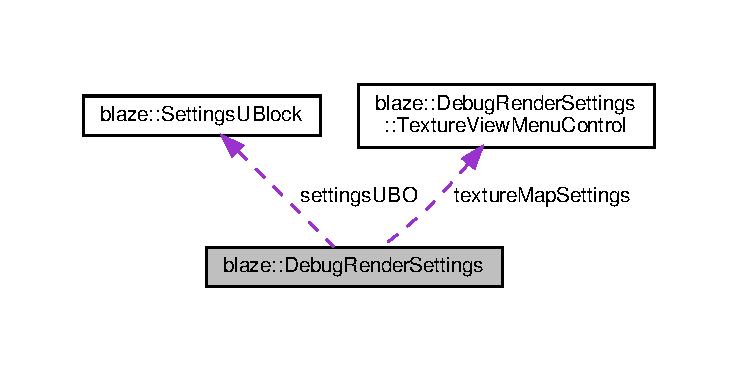
\includegraphics[width=350pt]{structblaze_1_1DebugRenderSettings__coll__graph}
\end{center}
\end{figure}
\subsection*{Classes}
\begin{DoxyCompactItemize}
\item 
struct \hyperlink{structblaze_1_1DebugRenderSettings_1_1TextureViewMenuControl}{Texture\+View\+Menu\+Control}
\end{DoxyCompactItemize}
\subsection*{Public Member Functions}
\begin{DoxyCompactItemize}
\item 
\mbox{\Hypertarget{structblaze_1_1DebugRenderSettings_aa8d60e20bb4e57f31f0cfc6f43d6aa95}\label{structblaze_1_1DebugRenderSettings_aa8d60e20bb4e57f31f0cfc6f43d6aa95}} 
void {\bfseries submit\+Delta} (float delta)
\end{DoxyCompactItemize}
\subsection*{Public Attributes}
\begin{DoxyCompactItemize}
\item 
\mbox{\Hypertarget{structblaze_1_1DebugRenderSettings_a168d29d8f6efde16789dbc8ab2a2283c}\label{structblaze_1_1DebugRenderSettings_a168d29d8f6efde16789dbc8ab2a2283c}} 
std\+::array$<$ float, 300 $>$ {\bfseries delta\+Time} \{0\}
\item 
\mbox{\Hypertarget{structblaze_1_1DebugRenderSettings_a2d3ca3891cef536948730d170c5984b8}\label{structblaze_1_1DebugRenderSettings_a2d3ca3891cef536948730d170c5984b8}} 
bool {\bfseries rotate} \{false\}
\item 
\mbox{\Hypertarget{structblaze_1_1DebugRenderSettings_a0e456c41c71fc3870d76327d10b913bb}\label{structblaze_1_1DebugRenderSettings_a0e456c41c71fc3870d76327d10b913bb}} 
float {\bfseries rotation\+Speed} \{1.\+0f\}
\item 
\mbox{\Hypertarget{structblaze_1_1DebugRenderSettings_a8bdec14f8d7eb62fa1232145b7c989b8}\label{structblaze_1_1DebugRenderSettings_a8bdec14f8d7eb62fa1232145b7c989b8}} 
glm\+::vec3 {\bfseries scale} \{1.\+0f\}
\item 
\mbox{\Hypertarget{structblaze_1_1DebugRenderSettings_aca85821e0ed410d4e6fe6e68c8c35a38}\label{structblaze_1_1DebugRenderSettings_aca85821e0ed410d4e6fe6e68c8c35a38}} 
char {\bfseries filename} \mbox{[}256\mbox{]} \{0\}
\item 
\mbox{\Hypertarget{structblaze_1_1DebugRenderSettings_ab5f8f297ec07ed32d02864862861adcd}\label{structblaze_1_1DebugRenderSettings_ab5f8f297ec07ed32d02864862861adcd}} 
char {\bfseries skybox} \mbox{[}256\mbox{]} \{0\}
\item 
\mbox{\Hypertarget{structblaze_1_1DebugRenderSettings_a2ab760f8e78d74c959bab3cf9d7ae512}\label{structblaze_1_1DebugRenderSettings_a2ab760f8e78d74c959bab3cf9d7ae512}} 
bool {\bfseries lock\+Light} \{false\}
\item 
\mbox{\Hypertarget{structblaze_1_1DebugRenderSettings_ac16b647cd5a79f88bb74c2a90630af40}\label{structblaze_1_1DebugRenderSettings_ac16b647cd5a79f88bb74c2a90630af40}} 
int {\bfseries current\+Light} \{0\}
\item 
\mbox{\Hypertarget{structblaze_1_1DebugRenderSettings_a336b29df42f5b248e263c08951a44246}\label{structblaze_1_1DebugRenderSettings_a336b29df42f5b248e263c08951a44246}} 
struct \hyperlink{structblaze_1_1DebugRenderSettings_1_1TextureViewMenuControl}{blaze\+::\+Debug\+Render\+Settings\+::\+Texture\+View\+Menu\+Control} {\bfseries texture\+Map\+Settings}
\item 
\mbox{\Hypertarget{structblaze_1_1DebugRenderSettings_acc93abf5152d147ac80bf0ab0233121e}\label{structblaze_1_1DebugRenderSettings_acc93abf5152d147ac80bf0ab0233121e}} 
\hyperlink{structblaze_1_1SettingsUBlock}{Settings\+U\+Block} {\bfseries settings\+U\+BO} = \{Settings\+U\+Block\+::\+V\+T\+M\+\_\+\+F\+U\+LL, 0, 0\}
\end{DoxyCompactItemize}


\subsection{Detailed Description}
Settings exposed during run using the \hyperlink{classblaze_1_1GUI}{G\+UI}. 

The documentation for this struct was generated from the following file\+:\begin{DoxyCompactItemize}
\item 
Blaze/Blaze.\+cpp\end{DoxyCompactItemize}

\hypertarget{structblaze_1_1vkw_1_1base_1_1DependentHolder}{}\section{blaze\+:\+:vkw\+:\+:base\+:\+:Dependent\+Holder$<$ T\+Handle, T\+Dep, T\+Destroy $>$ Struct Template Reference}
\label{structblaze_1_1vkw_1_1base_1_1DependentHolder}\index{blaze\+::vkw\+::base\+::\+Dependent\+Holder$<$ T\+Handle, T\+Dep, T\+Destroy $>$@{blaze\+::vkw\+::base\+::\+Dependent\+Holder$<$ T\+Handle, T\+Dep, T\+Destroy $>$}}


The most important wrapper to wrap handles that require some dependency to be used to deallocate.  




{\ttfamily \#include $<$Vk\+Wrap\+Base.\+hpp$>$}

\subsection*{Public Member Functions}
\begin{DoxyCompactItemize}
\item 
\mbox{\Hypertarget{structblaze_1_1vkw_1_1base_1_1DependentHolder_a1ed19fa0798e21238065d1cb3f600ca5}\label{structblaze_1_1vkw_1_1base_1_1DependentHolder_a1ed19fa0798e21238065d1cb3f600ca5}} 
{\bfseries Dependent\+Holder} (T\+Handle handle, T\+Dep dependency) noexcept
\item 
\mbox{\Hypertarget{structblaze_1_1vkw_1_1base_1_1DependentHolder_a9da72f8dc993cc3d118c81c149a27f89}\label{structblaze_1_1vkw_1_1base_1_1DependentHolder_a9da72f8dc993cc3d118c81c149a27f89}} 
{\bfseries Dependent\+Holder} (const \hyperlink{structblaze_1_1vkw_1_1base_1_1DependentHolder}{Dependent\+Holder} \&other)=delete
\item 
\mbox{\Hypertarget{structblaze_1_1vkw_1_1base_1_1DependentHolder_a3d080f63125b31555a302f95c6c5b8fd}\label{structblaze_1_1vkw_1_1base_1_1DependentHolder_a3d080f63125b31555a302f95c6c5b8fd}} 
\hyperlink{structblaze_1_1vkw_1_1base_1_1DependentHolder}{Dependent\+Holder} \& {\bfseries operator=} (const \hyperlink{structblaze_1_1vkw_1_1base_1_1DependentHolder}{Dependent\+Holder} \&other)=delete
\item 
\mbox{\Hypertarget{structblaze_1_1vkw_1_1base_1_1DependentHolder_a3acc433104c31698c760ddcad583839f}\label{structblaze_1_1vkw_1_1base_1_1DependentHolder_a3acc433104c31698c760ddcad583839f}} 
{\bfseries Dependent\+Holder} (\hyperlink{structblaze_1_1vkw_1_1base_1_1DependentHolder}{Dependent\+Holder} \&\&other) noexcept
\item 
\mbox{\Hypertarget{structblaze_1_1vkw_1_1base_1_1DependentHolder_a3f78bf0cdac98d49796f3af32eb6393f}\label{structblaze_1_1vkw_1_1base_1_1DependentHolder_a3f78bf0cdac98d49796f3af32eb6393f}} 
\hyperlink{structblaze_1_1vkw_1_1base_1_1DependentHolder}{Dependent\+Holder} \& {\bfseries operator=} (\hyperlink{structblaze_1_1vkw_1_1base_1_1DependentHolder}{Dependent\+Holder} \&\&other) noexcept
\item 
\mbox{\Hypertarget{structblaze_1_1vkw_1_1base_1_1DependentHolder_ac36f1b078ef4e6fb08be34ebc1101679}\label{structblaze_1_1vkw_1_1base_1_1DependentHolder_ac36f1b078ef4e6fb08be34ebc1101679}} 
const T\+Handle \& {\bfseries get} () const
\item 
\mbox{\Hypertarget{structblaze_1_1vkw_1_1base_1_1DependentHolder_a1349c85effef6bbfd027c43603fa4685}\label{structblaze_1_1vkw_1_1base_1_1DependentHolder_a1349c85effef6bbfd027c43603fa4685}} 
bool {\bfseries valid} () const
\end{DoxyCompactItemize}
\subsection*{Public Attributes}
\begin{DoxyCompactItemize}
\item 
\mbox{\Hypertarget{structblaze_1_1vkw_1_1base_1_1DependentHolder_a880cec3d6c3f427a492372e0a7fe2589}\label{structblaze_1_1vkw_1_1base_1_1DependentHolder_a880cec3d6c3f427a492372e0a7fe2589}} 
T\+Handle {\bfseries handle} \{V\+K\+\_\+\+N\+U\+L\+L\+\_\+\+H\+A\+N\+D\+LE\}
\item 
\mbox{\Hypertarget{structblaze_1_1vkw_1_1base_1_1DependentHolder_abfec06cf5378b9e9263f1e3f335eeb93}\label{structblaze_1_1vkw_1_1base_1_1DependentHolder_abfec06cf5378b9e9263f1e3f335eeb93}} 
T\+Dep {\bfseries dependency} \{V\+K\+\_\+\+N\+U\+L\+L\+\_\+\+H\+A\+N\+D\+LE\}
\end{DoxyCompactItemize}


\subsection{Detailed Description}
\subsubsection*{template$<$typename T\+Handle, typename T\+Dep, void($\ast$)(\+T\+Dep, T\+Handle, const Vk\+Allocation\+Callbacks $\ast$) T\+Destroy$>$\newline
struct blaze\+::vkw\+::base\+::\+Dependent\+Holder$<$ T\+Handle, T\+Dep, T\+Destroy $>$}

The most important wrapper to wrap handles that require some dependency to be used to deallocate. 

The dependency handle is not owned, while the handle is owned by the wrapper. At destruction, the relevant passed destructor will be called.


\begin{DoxyTemplParams}{Template Parameters}
{\em T\+Handle} & Type of handle \\
\hline
{\em T\+Dep} & The Type of handle of dependency. \\
\hline
{\em T\+Destroy} & The destroy function. \\
\hline
\end{DoxyTemplParams}


The documentation for this struct was generated from the following file\+:\begin{DoxyCompactItemize}
\item 
Blaze/vkwrap/Vk\+Wrap\+Base.\+hpp\end{DoxyCompactItemize}

\hypertarget{structblaze_1_1vkw_1_1base_1_1DeviceDependentVector}{}\section{blaze\+:\+:vkw\+:\+:base\+:\+:Device\+Dependent\+Vector$<$ T\+Handle, T\+Destroy $>$ Struct Template Reference}
\label{structblaze_1_1vkw_1_1base_1_1DeviceDependentVector}\index{blaze\+::vkw\+::base\+::\+Device\+Dependent\+Vector$<$ T\+Handle, T\+Destroy $>$@{blaze\+::vkw\+::base\+::\+Device\+Dependent\+Vector$<$ T\+Handle, T\+Destroy $>$}}


A vector version of Dependency\+Handler with a Vk\+Device dependency.  




{\ttfamily \#include $<$Vk\+Wrap\+Base.\+hpp$>$}

\subsection*{Public Member Functions}
\begin{DoxyCompactItemize}
\item 
\mbox{\Hypertarget{structblaze_1_1vkw_1_1base_1_1DeviceDependentVector_abe90751a1103c60604aec58eee935254}\label{structblaze_1_1vkw_1_1base_1_1DeviceDependentVector_abe90751a1103c60604aec58eee935254}} 
{\bfseries Device\+Dependent\+Vector} (std\+::vector$<$ T\+Handle $>$ \&\&col, Vk\+Device device) noexcept
\item 
\mbox{\Hypertarget{structblaze_1_1vkw_1_1base_1_1DeviceDependentVector_a2c56d257e7ff648ace2d6a9c69e382fb}\label{structblaze_1_1vkw_1_1base_1_1DeviceDependentVector_a2c56d257e7ff648ace2d6a9c69e382fb}} 
{\bfseries Device\+Dependent\+Vector} (const \hyperlink{structblaze_1_1vkw_1_1base_1_1DeviceDependentVector}{Device\+Dependent\+Vector} \&other)=delete
\item 
\mbox{\Hypertarget{structblaze_1_1vkw_1_1base_1_1DeviceDependentVector_a681e728084d947ddd3436f8c2ff7a886}\label{structblaze_1_1vkw_1_1base_1_1DeviceDependentVector_a681e728084d947ddd3436f8c2ff7a886}} 
\hyperlink{structblaze_1_1vkw_1_1base_1_1DeviceDependentVector}{Device\+Dependent\+Vector} \& {\bfseries operator=} (const \hyperlink{structblaze_1_1vkw_1_1base_1_1DeviceDependentVector}{Device\+Dependent\+Vector} \&other)=delete
\item 
\mbox{\Hypertarget{structblaze_1_1vkw_1_1base_1_1DeviceDependentVector_ac975f9eef1083c90b6e68438b8a8e7eb}\label{structblaze_1_1vkw_1_1base_1_1DeviceDependentVector_ac975f9eef1083c90b6e68438b8a8e7eb}} 
{\bfseries Device\+Dependent\+Vector} (\hyperlink{structblaze_1_1vkw_1_1base_1_1DeviceDependentVector}{Device\+Dependent\+Vector} \&\&other) noexcept
\item 
\mbox{\Hypertarget{structblaze_1_1vkw_1_1base_1_1DeviceDependentVector_a8b0780eeec6261857104165255ca61b7}\label{structblaze_1_1vkw_1_1base_1_1DeviceDependentVector_a8b0780eeec6261857104165255ca61b7}} 
\hyperlink{structblaze_1_1vkw_1_1base_1_1DeviceDependentVector}{Device\+Dependent\+Vector} \& {\bfseries operator=} (\hyperlink{structblaze_1_1vkw_1_1base_1_1DeviceDependentVector}{Device\+Dependent\+Vector} \&\&other) noexcept
\item 
\mbox{\Hypertarget{structblaze_1_1vkw_1_1base_1_1DeviceDependentVector_ae2db700663b306b10a6789db01e46673}\label{structblaze_1_1vkw_1_1base_1_1DeviceDependentVector_ae2db700663b306b10a6789db01e46673}} 
const std\+::vector$<$ T\+Handle $>$ \& {\bfseries get} () const
\item 
\mbox{\Hypertarget{structblaze_1_1vkw_1_1base_1_1DeviceDependentVector_a2f32b226bb32ae1c6a17f2a4f3ce5928}\label{structblaze_1_1vkw_1_1base_1_1DeviceDependentVector_a2f32b226bb32ae1c6a17f2a4f3ce5928}} 
const T\+Handle \& {\bfseries operator\mbox{[}$\,$\mbox{]}} (uint32\+\_\+t idx) const
\item 
\mbox{\Hypertarget{structblaze_1_1vkw_1_1base_1_1DeviceDependentVector_a37d08e0fd17b1c72cc29ced8e193c411}\label{structblaze_1_1vkw_1_1base_1_1DeviceDependentVector_a37d08e0fd17b1c72cc29ced8e193c411}} 
uint32\+\_\+t {\bfseries size} () const
\item 
\mbox{\Hypertarget{structblaze_1_1vkw_1_1base_1_1DeviceDependentVector_a08fbc01614054db54de510a4a85323fd}\label{structblaze_1_1vkw_1_1base_1_1DeviceDependentVector_a08fbc01614054db54de510a4a85323fd}} 
bool {\bfseries valid} () const
\end{DoxyCompactItemize}
\subsection*{Public Attributes}
\begin{DoxyCompactItemize}
\item 
\mbox{\Hypertarget{structblaze_1_1vkw_1_1base_1_1DeviceDependentVector_ad413ae2c074ca24d70b0b3c5e4e58a6e}\label{structblaze_1_1vkw_1_1base_1_1DeviceDependentVector_ad413ae2c074ca24d70b0b3c5e4e58a6e}} 
std\+::vector$<$ T\+Handle $>$ {\bfseries handles}
\item 
\mbox{\Hypertarget{structblaze_1_1vkw_1_1base_1_1DeviceDependentVector_a413a1eb0a0c780d44dafc19550946e40}\label{structblaze_1_1vkw_1_1base_1_1DeviceDependentVector_a413a1eb0a0c780d44dafc19550946e40}} 
Vk\+Device {\bfseries device} \{V\+K\+\_\+\+N\+U\+L\+L\+\_\+\+H\+A\+N\+D\+LE\}
\end{DoxyCompactItemize}


\subsection{Detailed Description}
\subsubsection*{template$<$typename T\+Handle, void($\ast$)(\+Vk\+Device, T\+Handle, const Vk\+Allocation\+Callbacks $\ast$) T\+Destroy$>$\newline
struct blaze\+::vkw\+::base\+::\+Device\+Dependent\+Vector$<$ T\+Handle, T\+Destroy $>$}

A vector version of Dependency\+Handler with a Vk\+Device dependency. 

Wrapper to own a collection of handles which require a Vk\+Device to be destroyed.


\begin{DoxyTemplParams}{Template Parameters}
{\em T\+Handle} & Type of handle. \\
\hline
{\em T\+Destroy} & The function for destroying the handle. \\
\hline
\end{DoxyTemplParams}


The documentation for this struct was generated from the following file\+:\begin{DoxyCompactItemize}
\item 
Blaze/vkwrap/Vk\+Wrap\+Base.\+hpp\end{DoxyCompactItemize}

\hypertarget{classDirectionalShadow}{}\section{Directional\+Shadow Class Reference}
\label{classDirectionalShadow}\index{Directional\+Shadow@{Directional\+Shadow}}


Encapsulates the attachments and framebuffer for a directional light shadow.  




{\ttfamily \#include $<$Light\+System.\+hpp$>$}



\subsection{Detailed Description}
Encapsulates the attachments and framebuffer for a directional light shadow. 

Contains the shadow\+Map/depth\+Map (D32) along with the framebuffer and viewport configured.

\begin{DoxyNote}{Note}
Not supposed to be used externally. 
\end{DoxyNote}


The documentation for this class was generated from the following file\+:\begin{DoxyCompactItemize}
\item 
Blaze/Light\+System.\+hpp\end{DoxyCompactItemize}

\hypertarget{classblaze_1_1Drawable}{}\section{blaze\+:\+:Drawable Interface Reference}
\label{classblaze_1_1Drawable}\index{blaze\+::\+Drawable@{blaze\+::\+Drawable}}


Interface for object that can be drawn by the renderer.  




{\ttfamily \#include $<$Drawable.\+hpp$>$}



Inheritance diagram for blaze\+:\+:Drawable\+:\nopagebreak
\begin{figure}[H]
\begin{center}
\leavevmode
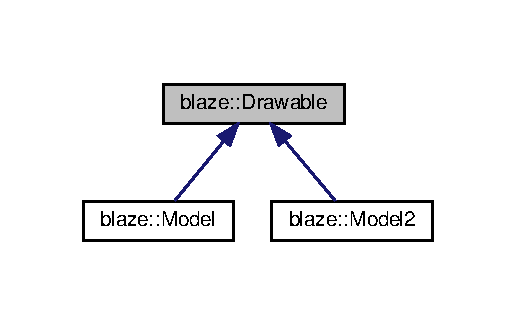
\includegraphics[width=248pt]{classblaze_1_1Drawable__inherit__graph}
\end{center}
\end{figure}
\subsection*{Public Member Functions}
\begin{DoxyCompactItemize}
\item 
virtual void \hyperlink{classblaze_1_1Drawable_a810b411ced93f27781a40a170714b590}{draw} (Vk\+Command\+Buffer cb, Vk\+Pipeline\+Layout lay)=0
\begin{DoxyCompactList}\small\item\em Should draw the model with all the material and maps included. \end{DoxyCompactList}\item 
virtual void \hyperlink{classblaze_1_1Drawable_aa2bd171547027319e4254c47e0628163}{draw\+Geometry} (Vk\+Command\+Buffer cb, Vk\+Pipeline\+Layout lay)=0
\begin{DoxyCompactList}\small\item\em Should draw only the geometry and not bind any materials. \end{DoxyCompactList}\end{DoxyCompactItemize}


\subsection{Detailed Description}
Interface for object that can be drawn by the renderer. 

\hyperlink{classblaze_1_1Renderer}{Renderer} contains two kinds of draws\+: \begin{DoxyItemize}
\item Full\+: Using material info. \item Geometry\+: Only using the vertex position. \end{DoxyItemize}


\subsection{Member Function Documentation}
\mbox{\Hypertarget{classblaze_1_1Drawable_a810b411ced93f27781a40a170714b590}\label{classblaze_1_1Drawable_a810b411ced93f27781a40a170714b590}} 
\index{blaze\+::\+Drawable@{blaze\+::\+Drawable}!draw@{draw}}
\index{draw@{draw}!blaze\+::\+Drawable@{blaze\+::\+Drawable}}
\subsubsection{\texorpdfstring{draw()}{draw()}}
{\footnotesize\ttfamily blaze\+::\+Drawable\+::draw (\begin{DoxyParamCaption}\item[{Vk\+Command\+Buffer}]{cb,  }\item[{Vk\+Pipeline\+Layout}]{lay }\end{DoxyParamCaption})\hspace{0.3cm}{\ttfamily [pure virtual]}}



Should draw the model with all the material and maps included. 

This method is used during the primary render and should bind all the required buffers and textures and push material P\+CB.


\begin{DoxyParams}{Parameters}
{\em cb} & The command buffer to record to. \\
\hline
{\em lay} & The pipeline layout to bind descriptors. \\
\hline
\end{DoxyParams}


Implemented in \hyperlink{classblaze_1_1Model2_a82bab7e2bed8bbbbff8f9c250785281d}{blaze\+::\+Model2}, and \hyperlink{classblaze_1_1Model_a00c3a74721bcad2d066de0c78313dae5}{blaze\+::\+Model}.

\mbox{\Hypertarget{classblaze_1_1Drawable_aa2bd171547027319e4254c47e0628163}\label{classblaze_1_1Drawable_aa2bd171547027319e4254c47e0628163}} 
\index{blaze\+::\+Drawable@{blaze\+::\+Drawable}!draw\+Geometry@{draw\+Geometry}}
\index{draw\+Geometry@{draw\+Geometry}!blaze\+::\+Drawable@{blaze\+::\+Drawable}}
\subsubsection{\texorpdfstring{draw\+Geometry()}{drawGeometry()}}
{\footnotesize\ttfamily blaze\+::\+Drawable\+::draw\+Geometry (\begin{DoxyParamCaption}\item[{Vk\+Command\+Buffer}]{cb,  }\item[{Vk\+Pipeline\+Layout}]{lay }\end{DoxyParamCaption})\hspace{0.3cm}{\ttfamily [pure virtual]}}



Should draw only the geometry and not bind any materials. 

This method is used for casting shadows and dowsn\textquotesingle{}t require any information beyond the position attribute of the \hyperlink{structblaze_1_1Vertex}{Vertex} and a model transformation P\+CB.


\begin{DoxyParams}{Parameters}
{\em cb} & The command buffer to record to. \\
\hline
{\em lay} & The pipeline layout to bind descriptors. \\
\hline
\end{DoxyParams}


Implemented in \hyperlink{classblaze_1_1Model2_aadf59268e6faa861e27d6995a63552c3}{blaze\+::\+Model2}, and \hyperlink{classblaze_1_1Model_ab5427d1b48ee3aedea9e405aa3892f5c}{blaze\+::\+Model}.



The documentation for this interface was generated from the following file\+:\begin{DoxyCompactItemize}
\item 
Blaze/core/Drawable.\+hpp\end{DoxyCompactItemize}

\hypertarget{classblaze_1_1util_1_1Environment}{}\section{blaze\+:\+:util\+:\+:Environment Class Reference}
\label{classblaze_1_1util_1_1Environment}\index{blaze\+::util\+::\+Environment@{blaze\+::util\+::\+Environment}}


Inheritance diagram for blaze\+:\+:util\+:\+:Environment\+:\nopagebreak
\begin{figure}[H]
\begin{center}
\leavevmode
\includegraphics[width=199pt]{classblaze_1_1util_1_1Environment__inherit__graph}
\end{center}
\end{figure}


Collaboration diagram for blaze\+:\+:util\+:\+:Environment\+:\nopagebreak
\begin{figure}[H]
\begin{center}
\leavevmode
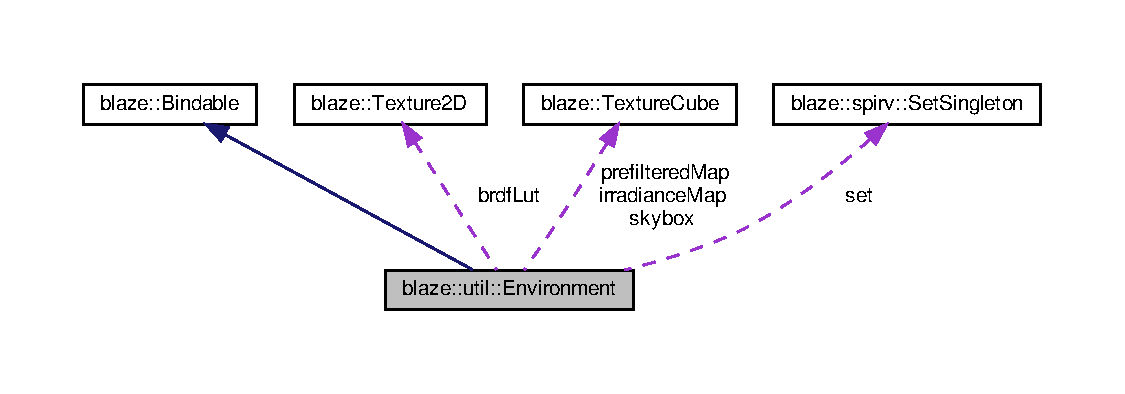
\includegraphics[width=350pt]{classblaze_1_1util_1_1Environment__coll__graph}
\end{center}
\end{figure}
\subsection*{Public Member Functions}
\begin{DoxyCompactItemize}
\item 
\mbox{\Hypertarget{classblaze_1_1util_1_1Environment_aa4f99d469e378ea8ab9d7fb3af343e11}\label{classblaze_1_1util_1_1Environment_aa4f99d469e378ea8ab9d7fb3af343e11}} 
{\bfseries Environment} (\hyperlink{classblaze_1_1ARenderer}{A\+Renderer} $\ast$renderer, \hyperlink{classblaze_1_1TextureCube}{Texture\+Cube} \&\&skybox)
\item 
\mbox{\Hypertarget{classblaze_1_1util_1_1Environment_a9a7be13c2be2c08d3b9a04d88ef1c3bd}\label{classblaze_1_1util_1_1Environment_a9a7be13c2be2c08d3b9a04d88ef1c3bd}} 
void {\bfseries bind} (Vk\+Command\+Buffer cmd\+Buf, Vk\+Pipeline\+Layout lay) const
\end{DoxyCompactItemize}
\subsection*{Public Attributes}
\begin{DoxyCompactItemize}
\item 
\mbox{\Hypertarget{classblaze_1_1util_1_1Environment_affa9b7f46e972eb0aaacd39aa4540429}\label{classblaze_1_1util_1_1Environment_affa9b7f46e972eb0aaacd39aa4540429}} 
\hyperlink{classblaze_1_1TextureCube}{Texture\+Cube} {\bfseries skybox}
\item 
\mbox{\Hypertarget{classblaze_1_1util_1_1Environment_ac275012db9cb9036002297de82d04ddd}\label{classblaze_1_1util_1_1Environment_ac275012db9cb9036002297de82d04ddd}} 
\hyperlink{classblaze_1_1TextureCube}{Texture\+Cube} {\bfseries irradiance\+Map}
\item 
\mbox{\Hypertarget{classblaze_1_1util_1_1Environment_a9098a6f07ad08dd4cff1be808f3d5cc0}\label{classblaze_1_1util_1_1Environment_a9098a6f07ad08dd4cff1be808f3d5cc0}} 
\hyperlink{classblaze_1_1TextureCube}{Texture\+Cube} {\bfseries prefiltered\+Map}
\item 
\mbox{\Hypertarget{classblaze_1_1util_1_1Environment_a749c7bf4dca2a7f7b62e6a755c506711}\label{classblaze_1_1util_1_1Environment_a749c7bf4dca2a7f7b62e6a755c506711}} 
\hyperlink{classblaze_1_1Texture2D}{Texture2D} {\bfseries brdf\+Lut}
\item 
\mbox{\Hypertarget{classblaze_1_1util_1_1Environment_a6b5e65e31781f21763ab5afa7779f536}\label{classblaze_1_1util_1_1Environment_a6b5e65e31781f21763ab5afa7779f536}} 
\hyperlink{structblaze_1_1spirv_1_1SetSingleton}{spirv\+::\+Set\+Singleton} {\bfseries set}
\end{DoxyCompactItemize}


The documentation for this class was generated from the following files\+:\begin{DoxyCompactItemize}
\item 
Blaze/util/Environment.\+hpp\item 
Blaze/util/Environment.\+cpp\end{DoxyCompactItemize}

\hypertarget{structblaze_1_1spirv_1_1Shader_1_1Set_1_1Format}{}\section{blaze\+:\+:spirv\+:\+:Shader\+:\+:Set\+:\+:Format Struct Reference}
\label{structblaze_1_1spirv_1_1Shader_1_1Set_1_1Format}\index{blaze\+::spirv\+::\+Shader\+::\+Set\+::\+Format@{blaze\+::spirv\+::\+Shader\+::\+Set\+::\+Format}}
\subsection*{Public Member Functions}
\begin{DoxyCompactItemize}
\item 
\mbox{\Hypertarget{structblaze_1_1spirv_1_1Shader_1_1Set_1_1Format_a8e92dcaeb1fbf5b471a8efe2307185eb}\label{structblaze_1_1spirv_1_1Shader_1_1Set_1_1Format_a8e92dcaeb1fbf5b471a8efe2307185eb}} 
bool {\bfseries operator$<$} (const \hyperlink{structblaze_1_1spirv_1_1Shader_1_1Set_1_1Format}{Format} \&other) const
\end{DoxyCompactItemize}
\subsection*{Public Attributes}
\begin{DoxyCompactItemize}
\item 
\mbox{\Hypertarget{structblaze_1_1spirv_1_1Shader_1_1Set_1_1Format_afc9fe2b5c8468a44d40ffe9dfc32c6f9}\label{structblaze_1_1spirv_1_1Shader_1_1Set_1_1Format_afc9fe2b5c8468a44d40ffe9dfc32c6f9}} 
std\+::vector$<$ \hyperlink{structblaze_1_1spirv_1_1UniformInfo}{Uniform\+Info} $>$ {\bfseries uniforms}
\end{DoxyCompactItemize}


The documentation for this struct was generated from the following file\+:\begin{DoxyCompactItemize}
\item 
Blaze/spirv/Pipeline.\+hpp\end{DoxyCompactItemize}

\hypertarget{structblaze_1_1spirv_1_1Framebuffer_1_1Format}{}\section{blaze\+:\+:spirv\+:\+:Framebuffer\+:\+:Format Struct Reference}
\label{structblaze_1_1spirv_1_1Framebuffer_1_1Format}\index{blaze\+::spirv\+::\+Framebuffer\+::\+Format@{blaze\+::spirv\+::\+Framebuffer\+::\+Format}}
\subsection*{Public Member Functions}
\begin{DoxyCompactItemize}
\item 
\mbox{\Hypertarget{structblaze_1_1spirv_1_1Framebuffer_1_1Format_a7179be170e4b1336623a9ce1dee1ed4a}\label{structblaze_1_1spirv_1_1Framebuffer_1_1Format_a7179be170e4b1336623a9ce1dee1ed4a}} 
bool {\bfseries operator$<$} (const \hyperlink{structblaze_1_1spirv_1_1Framebuffer_1_1Format}{Format} \&other) const
\end{DoxyCompactItemize}
\subsection*{Public Attributes}
\begin{DoxyCompactItemize}
\item 
\mbox{\Hypertarget{structblaze_1_1spirv_1_1Framebuffer_1_1Format_a6152082caafb384ed546fc9188d40c3d}\label{structblaze_1_1spirv_1_1Framebuffer_1_1Format_a6152082caafb384ed546fc9188d40c3d}} 
std\+::vector$<$ \hyperlink{structblaze_1_1spirv_1_1AttachmentFormat}{Attachment\+Format} $>$ {\bfseries attachment\+Formats}
\end{DoxyCompactItemize}


The documentation for this struct was generated from the following file\+:\begin{DoxyCompactItemize}
\item 
Blaze/spirv/Pipeline\+Factory.\+hpp\end{DoxyCompactItemize}

\hypertarget{classblaze_1_1ForwardRenderer}{}\section{blaze\+:\+:Forward\+Renderer Class Reference}
\label{classblaze_1_1ForwardRenderer}\index{blaze\+::\+Forward\+Renderer@{blaze\+::\+Forward\+Renderer}}


Contains entire rendering logic.  




{\ttfamily \#include $<$Forward\+Renderer.\+hpp$>$}



Inheritance diagram for blaze\+:\+:Forward\+Renderer\+:\nopagebreak
\begin{figure}[H]
\begin{center}
\leavevmode
\includegraphics[width=201pt]{classblaze_1_1ForwardRenderer__inherit__graph}
\end{center}
\end{figure}


Collaboration diagram for blaze\+:\+:Forward\+Renderer\+:\nopagebreak
\begin{figure}[H]
\begin{center}
\leavevmode
\includegraphics[width=201pt]{classblaze_1_1ForwardRenderer__coll__graph}
\end{center}
\end{figure}
\subsection*{Public Member Functions}
\begin{DoxyCompactItemize}
\item 
\mbox{\Hypertarget{classblaze_1_1ForwardRenderer_afdb79d0a5f62e871d166f0e621520a5d}\label{classblaze_1_1ForwardRenderer_afdb79d0a5f62e871d166f0e621520a5d}} 
\hyperlink{classblaze_1_1ForwardRenderer_afdb79d0a5f62e871d166f0e621520a5d}{Forward\+Renderer} () noexcept
\begin{DoxyCompactList}\small\item\em Default empty constructor. \end{DoxyCompactList}\item 
\hyperlink{classblaze_1_1ForwardRenderer_abf0b80128aa61686461b3069004b65a9}{Forward\+Renderer} (G\+L\+F\+Wwindow $\ast$window, bool enable\+Validation\+Layers=true) noexcept
\begin{DoxyCompactList}\small\item\em Actual constructor. \end{DoxyCompactList}\item 
\mbox{\Hypertarget{classblaze_1_1ForwardRenderer_ae547518efb38283e0111899bccabbe9f}\label{classblaze_1_1ForwardRenderer_ae547518efb38283e0111899bccabbe9f}} 
void \hyperlink{classblaze_1_1ForwardRenderer_ae547518efb38283e0111899bccabbe9f}{render\+Frame} ()
\begin{DoxyCompactList}\small\item\em Actually rendering a frame and submitting to the present queue. \end{DoxyCompactList}\item 
\mbox{\Hypertarget{classblaze_1_1ForwardRenderer_acfacb0d44b7f1f1f90bbdbeb762c0ac0}\label{classblaze_1_1ForwardRenderer_acfacb0d44b7f1f1f90bbdbeb762c0ac0}} 
H\+Sub \hyperlink{classblaze_1_1ForwardRenderer_acfacb0d44b7f1f1f90bbdbeb762c0ac0}{submit} (\hyperlink{classblaze_1_1Drawable}{Drawable} $\ast$cmd)
\begin{DoxyCompactList}\small\item\em Submits a \hyperlink{classblaze_1_1Drawable}{Drawable} to draw to screen. \end{DoxyCompactList}\item 
bool \hyperlink{classblaze_1_1ForwardRenderer_a78175e4b430f0046db968f8476ec121c}{complete} () const
\begin{DoxyCompactList}\small\item\em Checks if the renderer is complete. \end{DoxyCompactList}\end{DoxyCompactItemize}
\begin{Indent}\textbf{ Move Constructors.}\par
{\em Move only, Copy is deleted. }\begin{DoxyCompactItemize}
\item 
\mbox{\Hypertarget{classblaze_1_1ForwardRenderer_a0a6c8cf08a058fe3fbd25b9ecdc3c28b}\label{classblaze_1_1ForwardRenderer_a0a6c8cf08a058fe3fbd25b9ecdc3c28b}} 
{\bfseries Forward\+Renderer} (\hyperlink{classblaze_1_1ForwardRenderer}{Forward\+Renderer} \&\&other) noexcept
\item 
\mbox{\Hypertarget{classblaze_1_1ForwardRenderer_a027a5ab5ab27a6248c40eaa57ecd140d}\label{classblaze_1_1ForwardRenderer_a027a5ab5ab27a6248c40eaa57ecd140d}} 
\hyperlink{classblaze_1_1ForwardRenderer}{Forward\+Renderer} \& {\bfseries operator=} (\hyperlink{classblaze_1_1ForwardRenderer}{Forward\+Renderer} \&\&other) noexcept
\item 
\mbox{\Hypertarget{classblaze_1_1ForwardRenderer_a6b60ffa32fc81b846ce05729e000693e}\label{classblaze_1_1ForwardRenderer_a6b60ffa32fc81b846ce05729e000693e}} 
{\bfseries Forward\+Renderer} (const \hyperlink{classblaze_1_1ForwardRenderer}{Forward\+Renderer} \&other)=delete
\item 
\mbox{\Hypertarget{classblaze_1_1ForwardRenderer_a3a9d723f9618259735a292a264ebcf05}\label{classblaze_1_1ForwardRenderer_a3a9d723f9618259735a292a264ebcf05}} 
\hyperlink{classblaze_1_1ForwardRenderer}{Forward\+Renderer} \& {\bfseries operator=} (const \hyperlink{classblaze_1_1ForwardRenderer}{Forward\+Renderer} \&other)=delete
\end{DoxyCompactItemize}
\end{Indent}
\begin{Indent}\textbf{ Getters}\par
{\em Getters for private members. }\begin{DoxyCompactItemize}
\item 
\mbox{\Hypertarget{classblaze_1_1ForwardRenderer_a871a10ee38277a2cb2c0ef9e3d65712f}\label{classblaze_1_1ForwardRenderer_a871a10ee38277a2cb2c0ef9e3d65712f}} 
std\+::pair$<$ uint32\+\_\+t, uint32\+\_\+t $>$ {\bfseries get\+\_\+dimensions} () const
\item 
\mbox{\Hypertarget{classblaze_1_1ForwardRenderer_ab0c14f3daed7186b1e726f7efd122e7d}\label{classblaze_1_1ForwardRenderer_ab0c14f3daed7186b1e726f7efd122e7d}} 
const Vk\+Format \& {\bfseries get\+\_\+swapchain\+Format} () const
\item 
\mbox{\Hypertarget{classblaze_1_1ForwardRenderer_ae4a6f9234ad9454acd3edafec772480e}\label{classblaze_1_1ForwardRenderer_ae4a6f9234ad9454acd3edafec772480e}} 
const Vk\+Extent2D \& {\bfseries get\+\_\+swapchain\+Extent} () const
\item 
\mbox{\Hypertarget{classblaze_1_1ForwardRenderer_afb27e80c004057dc8aec9652d160e53b}\label{classblaze_1_1ForwardRenderer_afb27e80c004057dc8aec9652d160e53b}} 
size\+\_\+t {\bfseries get\+\_\+swapchain\+Image\+Count} () const
\item 
\mbox{\Hypertarget{classblaze_1_1ForwardRenderer_aa442b4f23e7db5f9650802a56bfc37f5}\label{classblaze_1_1ForwardRenderer_aa442b4f23e7db5f9650802a56bfc37f5}} 
const Vk\+Image\+View \& {\bfseries get\+\_\+swapchain\+Image\+View} (uint32\+\_\+t index) const
\item 
\mbox{\Hypertarget{classblaze_1_1ForwardRenderer_a3f103d7524870ec1bc7b8a1a9ee9d85f}\label{classblaze_1_1ForwardRenderer_a3f103d7524870ec1bc7b8a1a9ee9d85f}} 
const std\+::vector$<$ Vk\+Image\+View $>$ \& {\bfseries get\+\_\+swapchain\+Image\+Views} () const
\item 
\mbox{\Hypertarget{classblaze_1_1ForwardRenderer_ae50e653d1321151a9f9c9809d660958c}\label{classblaze_1_1ForwardRenderer_ae50e653d1321151a9f9c9809d660958c}} 
const Vk\+Render\+Pass \& {\bfseries get\+\_\+render\+Pass} () const
\item 
\mbox{\Hypertarget{classblaze_1_1ForwardRenderer_afb5a01c431387ae87f2b69f1a95faa0a}\label{classblaze_1_1ForwardRenderer_afb5a01c431387ae87f2b69f1a95faa0a}} 
const Vk\+Pipeline \& {\bfseries get\+\_\+graphics\+Pipeline} () const
\item 
\mbox{\Hypertarget{classblaze_1_1ForwardRenderer_aa13a6c13d0688cafd96aecf19dce466c}\label{classblaze_1_1ForwardRenderer_aa13a6c13d0688cafd96aecf19dce466c}} 
size\+\_\+t {\bfseries get\+\_\+framebuffer\+Count} () const
\item 
\mbox{\Hypertarget{classblaze_1_1ForwardRenderer_a269ca18ba0efb64bb895a9c179a9c4e0}\label{classblaze_1_1ForwardRenderer_a269ca18ba0efb64bb895a9c179a9c4e0}} 
const Vk\+Framebuffer \& {\bfseries get\+\_\+framebuffer} (size\+\_\+t index) const
\item 
\mbox{\Hypertarget{classblaze_1_1ForwardRenderer_a39079fb0955406b7d080a8768a518d82}\label{classblaze_1_1ForwardRenderer_a39079fb0955406b7d080a8768a518d82}} 
size\+\_\+t {\bfseries get\+\_\+command\+Buffer\+Count} () const
\item 
\mbox{\Hypertarget{classblaze_1_1ForwardRenderer_ae55781002a3ab027efc89513559bd848}\label{classblaze_1_1ForwardRenderer_ae55781002a3ab027efc89513559bd848}} 
const Vk\+Command\+Buffer \& {\bfseries get\+\_\+command\+Buffer} (size\+\_\+t index) const
\item 
\mbox{\Hypertarget{classblaze_1_1ForwardRenderer_a81ce45e3acc00ec286bfa2fa17d0bc4a}\label{classblaze_1_1ForwardRenderer_a81ce45e3acc00ec286bfa2fa17d0bc4a}} 
const Vk\+Descriptor\+Set\+Layout \& {\bfseries get\+\_\+ubo\+Layout} () const
\item 
\mbox{\Hypertarget{classblaze_1_1ForwardRenderer_af15b7613cd44e32ef27128766eaa5fc5}\label{classblaze_1_1ForwardRenderer_af15b7613cd44e32ef27128766eaa5fc5}} 
const Vk\+Descriptor\+Set\+Layout \& {\bfseries get\+\_\+material\+Layout} () const
\item 
\mbox{\Hypertarget{classblaze_1_1ForwardRenderer_a76cad25fcb3b9f08e0fa257c9f2b9e94}\label{classblaze_1_1ForwardRenderer_a76cad25fcb3b9f08e0fa257c9f2b9e94}} 
const Vk\+Descriptor\+Set\+Layout \& {\bfseries get\+\_\+environment\+Layout} () const
\item 
\mbox{\Hypertarget{classblaze_1_1ForwardRenderer_a68211e939eaba2537bc51df33cc35823}\label{classblaze_1_1ForwardRenderer_a68211e939eaba2537bc51df33cc35823}} 
\hyperlink{classblaze_1_1LightSystem}{Light\+System} \& {\bfseries get\+\_\+light\+System} ()
\item 
\mbox{\Hypertarget{classblaze_1_1ForwardRenderer_a9dab699dc44eb3b2fb21fe4d1c55f04b}\label{classblaze_1_1ForwardRenderer_a9dab699dc44eb3b2fb21fe4d1c55f04b}} 
Vk\+Device {\bfseries get\+\_\+device} () const
\item 
\mbox{\Hypertarget{classblaze_1_1ForwardRenderer_ad650c175a5b4d01fbae664dc7923fba2}\label{classblaze_1_1ForwardRenderer_ad650c175a5b4d01fbae664dc7923fba2}} 
Vk\+Physical\+Device {\bfseries get\+\_\+physical\+Device} () const
\item 
\mbox{\Hypertarget{classblaze_1_1ForwardRenderer_adc1a5b6c9a65095ff8522700299bf01f}\label{classblaze_1_1ForwardRenderer_adc1a5b6c9a65095ff8522700299bf01f}} 
Vk\+Queue {\bfseries get\+\_\+transfer\+Queue} () const
\item 
\mbox{\Hypertarget{classblaze_1_1ForwardRenderer_a621f7347a28af51ab7cd058a0d87526d}\label{classblaze_1_1ForwardRenderer_a621f7347a28af51ab7cd058a0d87526d}} 
Vk\+Command\+Pool {\bfseries get\+\_\+transfer\+Command\+Pool} () const
\item 
\mbox{\Hypertarget{classblaze_1_1ForwardRenderer_a4e4c901e8abac21a3004cb21efe76ffa}\label{classblaze_1_1ForwardRenderer_a4e4c901e8abac21a3004cb21efe76ffa}} 
const \hyperlink{classblaze_1_1Context}{Context} \& {\bfseries get\+\_\+context} () const
\end{DoxyCompactItemize}
\end{Indent}
\begin{Indent}\textbf{ Setters}\par
{\em Setters for various properties. }\begin{DoxyCompactItemize}
\item 
\mbox{\Hypertarget{classblaze_1_1ForwardRenderer_aa3efcc09e6fa7bd7d24852e1604dc74a}\label{classblaze_1_1ForwardRenderer_aa3efcc09e6fa7bd7d24852e1604dc74a}} 
void {\bfseries set\+\_\+environment\+Descriptor} (Vk\+Descriptor\+Set env\+DS)
\item 
\mbox{\Hypertarget{classblaze_1_1ForwardRenderer_a350c02de6852b53cd716d2bd658ae6ba}\label{classblaze_1_1ForwardRenderer_a350c02de6852b53cd716d2bd658ae6ba}} 
void {\bfseries set\+\_\+skybox\+Command} (const Render\+Command \&cmd)
\item 
\mbox{\Hypertarget{classblaze_1_1ForwardRenderer_ad803f802a4c790f3eace6478b40ada10}\label{classblaze_1_1ForwardRenderer_ad803f802a4c790f3eace6478b40ada10}} 
void {\bfseries set\+\_\+camera\+U\+BO} (const \hyperlink{structblaze_1_1CameraUBlock}{Camera\+U\+Block} \&ubo)
\item 
\mbox{\Hypertarget{classblaze_1_1ForwardRenderer_aee7c41ff828dca60051e49b512621bb4}\label{classblaze_1_1ForwardRenderer_aee7c41ff828dca60051e49b512621bb4}} 
void {\bfseries set\+\_\+camera} (\hyperlink{classblaze_1_1Camera}{Camera} $\ast$cam)
\item 
\mbox{\Hypertarget{classblaze_1_1ForwardRenderer_a9859c881ae01d21f8b9be2660d8b02bc}\label{classblaze_1_1ForwardRenderer_a9859c881ae01d21f8b9be2660d8b02bc}} 
void {\bfseries set\+\_\+light\+U\+BO} (const \hyperlink{structblaze_1_1LightsUBlock}{Lights\+U\+Block} \&ubo)
\item 
\mbox{\Hypertarget{classblaze_1_1ForwardRenderer_ac70cb2eea41211cf964e883cfe663e9b}\label{classblaze_1_1ForwardRenderer_ac70cb2eea41211cf964e883cfe663e9b}} 
void {\bfseries set\+\_\+settings\+U\+BO} (const \hyperlink{structblaze_1_1SettingsUBlock}{Settings\+U\+Block} \&ubo)
\end{DoxyCompactItemize}
\end{Indent}
\subsection*{Additional Inherited Members}


\subsection{Detailed Description}
Contains entire rendering logic. 

This class contains the main drawing logic and all the related components. This is a forward renderer that supports P\+BR rendering. 

\subsection{Constructor \& Destructor Documentation}
\mbox{\Hypertarget{classblaze_1_1ForwardRenderer_abf0b80128aa61686461b3069004b65a9}\label{classblaze_1_1ForwardRenderer_abf0b80128aa61686461b3069004b65a9}} 
\index{blaze\+::\+Forward\+Renderer@{blaze\+::\+Forward\+Renderer}!Forward\+Renderer@{Forward\+Renderer}}
\index{Forward\+Renderer@{Forward\+Renderer}!blaze\+::\+Forward\+Renderer@{blaze\+::\+Forward\+Renderer}}
\subsubsection{\texorpdfstring{Forward\+Renderer()}{ForwardRenderer()}}
{\footnotesize\ttfamily blaze\+::\+Forward\+Renderer\+::\+Forward\+Renderer (\begin{DoxyParamCaption}\item[{G\+L\+F\+Wwindow $\ast$}]{window,  }\item[{bool}]{enable\+Validation\+Layers = {\ttfamily true} }\end{DoxyParamCaption})\hspace{0.3cm}{\ttfamily [noexcept]}}



Actual constructor. 


\begin{DoxyParams}{Parameters}
{\em window} & The G\+L\+FW window pointer. \\
\hline
{\em enable\+Validation\+Layers} & Enable for Debugging. \\
\hline
\end{DoxyParams}


\subsection{Member Function Documentation}
\mbox{\Hypertarget{classblaze_1_1ForwardRenderer_a78175e4b430f0046db968f8476ec121c}\label{classblaze_1_1ForwardRenderer_a78175e4b430f0046db968f8476ec121c}} 
\index{blaze\+::\+Forward\+Renderer@{blaze\+::\+Forward\+Renderer}!complete@{complete}}
\index{complete@{complete}!blaze\+::\+Forward\+Renderer@{blaze\+::\+Forward\+Renderer}}
\subsubsection{\texorpdfstring{complete()}{complete()}}
{\footnotesize\ttfamily blaze\+::\+Forward\+Renderer\+::complete (\begin{DoxyParamCaption}{ }\end{DoxyParamCaption}) const\hspace{0.3cm}{\ttfamily [inline]}, {\ttfamily [virtual]}}



Checks if the renderer is complete. 

A \hyperlink{classblaze_1_1ForwardRenderer}{Forward\+Renderer} is considered complete if and only if every member is initialized.

\begin{DoxyReturn}{Returns}
{\itshape true} If the renderer sucessfully initialized 

{\itshape false} If the renderer was empty or had initialization errors. 
\end{DoxyReturn}


Implements \hyperlink{classblaze_1_1Renderer}{blaze\+::\+Renderer}.



The documentation for this class was generated from the following files\+:\begin{DoxyCompactItemize}
\item 
Blaze/rendering/Forward\+Renderer.\+hpp\item 
Blaze/rendering/Forward\+Renderer.\+cpp\end{DoxyCompactItemize}

\hypertarget{structblaze_1_1spirv_1_1Framebuffer}{}\section{blaze\+:\+:spirv\+:\+:Framebuffer Struct Reference}
\label{structblaze_1_1spirv_1_1Framebuffer}\index{blaze\+::spirv\+::\+Framebuffer@{blaze\+::spirv\+::\+Framebuffer}}
\subsection*{Classes}
\begin{DoxyCompactItemize}
\item 
struct \hyperlink{structblaze_1_1spirv_1_1Framebuffer_1_1Format}{Format}
\end{DoxyCompactItemize}
\subsection*{Public Types}
\begin{DoxyCompactItemize}
\item 
\mbox{\Hypertarget{structblaze_1_1spirv_1_1Framebuffer_a58e3008a8d8bf821270ff320fbfe9743}\label{structblaze_1_1spirv_1_1Framebuffer_a58e3008a8d8bf821270ff320fbfe9743}} 
using {\bfseries Format\+ID} = uint32\+\_\+t
\end{DoxyCompactItemize}


The documentation for this struct was generated from the following file\+:\begin{DoxyCompactItemize}
\item 
Blaze/spirv/Pipeline\+Factory.\+hpp\end{DoxyCompactItemize}

\hypertarget{classblaze_1_1FwdRenderer}{}\section{blaze\+:\+:Fwd\+Renderer Class Reference}
\label{classblaze_1_1FwdRenderer}\index{blaze\+::\+Fwd\+Renderer@{blaze\+::\+Fwd\+Renderer}}


Inheritance diagram for blaze\+:\+:Fwd\+Renderer\+:\nopagebreak
\begin{figure}[H]
\begin{center}
\leavevmode
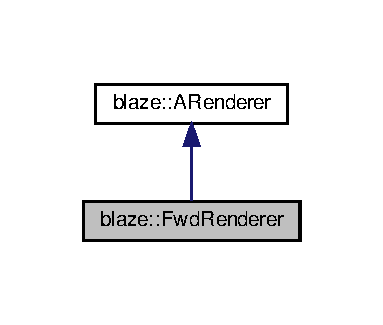
\includegraphics[width=184pt]{classblaze_1_1FwdRenderer__inherit__graph}
\end{center}
\end{figure}


Collaboration diagram for blaze\+:\+:Fwd\+Renderer\+:\nopagebreak
\begin{figure}[H]
\begin{center}
\leavevmode
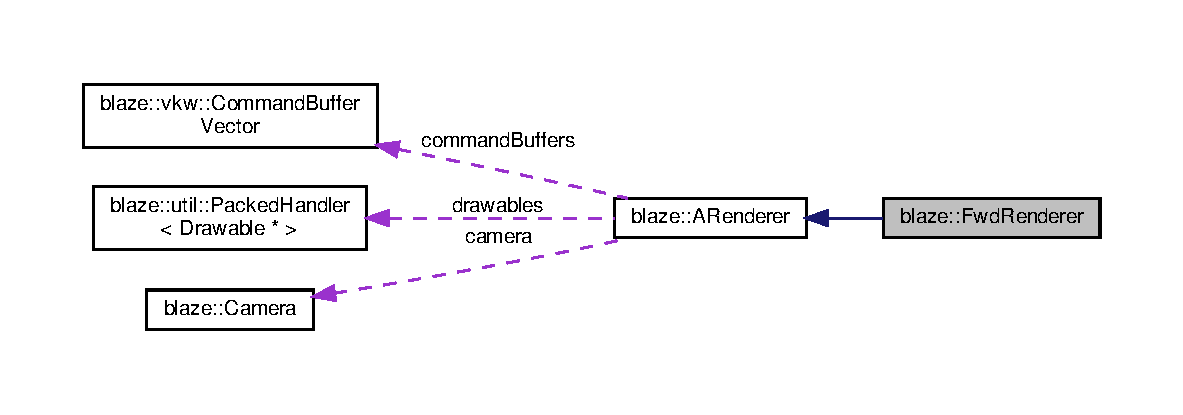
\includegraphics[width=350pt]{classblaze_1_1FwdRenderer__coll__graph}
\end{center}
\end{figure}
\subsection*{Public Member Functions}
\begin{DoxyCompactItemize}
\item 
\mbox{\Hypertarget{classblaze_1_1FwdRenderer_a9144b4500d80c3cc784506f9930f9fbc}\label{classblaze_1_1FwdRenderer_a9144b4500d80c3cc784506f9930f9fbc}} 
\hyperlink{classblaze_1_1FwdRenderer_a9144b4500d80c3cc784506f9930f9fbc}{Fwd\+Renderer} () noexcept
\begin{DoxyCompactList}\small\item\em Default empty constructor. \end{DoxyCompactList}\item 
\hyperlink{classblaze_1_1FwdRenderer_a4930aa617bc159adf645bce6ff5866a5}{Fwd\+Renderer} (G\+L\+F\+Wwindow $\ast$window, bool enable\+Validation\+Layers=true) noexcept
\begin{DoxyCompactList}\small\item\em Actual constructor. \end{DoxyCompactList}\item 
\mbox{\Hypertarget{classblaze_1_1FwdRenderer_a322489ddcd20fa21a14cae91b37caf5f}\label{classblaze_1_1FwdRenderer_a322489ddcd20fa21a14cae91b37caf5f}} 
virtual \hyperlink{structblaze_1_1spirv_1_1SetSingleton}{spirv\+::\+Set\+Singleton} {\bfseries create\+Material\+Set} () override
\item 
\mbox{\Hypertarget{classblaze_1_1FwdRenderer_afdfe27f7255e4b8f8ed1333e0180fa03}\label{classblaze_1_1FwdRenderer_afdfe27f7255e4b8f8ed1333e0180fa03}} 
virtual const \hyperlink{structblaze_1_1spirv_1_1Shader}{spirv\+::\+Shader} \& {\bfseries get\+\_\+shader} () const override
\end{DoxyCompactItemize}
\begin{Indent}\textbf{ Constructors.}\par
{\em Pointer use only. }\begin{DoxyCompactItemize}
\item 
\mbox{\Hypertarget{classblaze_1_1FwdRenderer_a0792c9fa2393260dab48fad131ad03f0}\label{classblaze_1_1FwdRenderer_a0792c9fa2393260dab48fad131ad03f0}} 
{\bfseries Fwd\+Renderer} (\hyperlink{classblaze_1_1FwdRenderer}{Fwd\+Renderer} \&\&other)=delete
\item 
\mbox{\Hypertarget{classblaze_1_1FwdRenderer_a15645403475fad4ec8c03dd3005237f6}\label{classblaze_1_1FwdRenderer_a15645403475fad4ec8c03dd3005237f6}} 
\hyperlink{classblaze_1_1FwdRenderer}{Fwd\+Renderer} \& {\bfseries operator=} (\hyperlink{classblaze_1_1FwdRenderer}{Fwd\+Renderer} \&\&other)=delete
\item 
\mbox{\Hypertarget{classblaze_1_1FwdRenderer_a0d31a6eca8dd011994b7a475230f352b}\label{classblaze_1_1FwdRenderer_a0d31a6eca8dd011994b7a475230f352b}} 
{\bfseries Fwd\+Renderer} (const \hyperlink{classblaze_1_1FwdRenderer}{Fwd\+Renderer} \&other)=delete
\item 
\mbox{\Hypertarget{classblaze_1_1FwdRenderer_acba62a051daf0002ad36325074e34bb1}\label{classblaze_1_1FwdRenderer_acba62a051daf0002ad36325074e34bb1}} 
\hyperlink{classblaze_1_1FwdRenderer}{Fwd\+Renderer} \& {\bfseries operator=} (const \hyperlink{classblaze_1_1FwdRenderer}{Fwd\+Renderer} \&other)=delete
\end{DoxyCompactItemize}
\end{Indent}
\subsection*{Protected Member Functions}
\begin{DoxyCompactItemize}
\item 
\mbox{\Hypertarget{classblaze_1_1FwdRenderer_ab402f10b76cc1f298b5c5df16a47ec4a}\label{classblaze_1_1FwdRenderer_ab402f10b76cc1f298b5c5df16a47ec4a}} 
virtual void {\bfseries update} (uint32\+\_\+t frame) override
\item 
\mbox{\Hypertarget{classblaze_1_1FwdRenderer_ac9f37fa5189aa08c5ee22348b404ed16}\label{classblaze_1_1FwdRenderer_ac9f37fa5189aa08c5ee22348b404ed16}} 
virtual void {\bfseries record\+Commands} (uint32\+\_\+t frame) override
\item 
\mbox{\Hypertarget{classblaze_1_1FwdRenderer_a991222407e69acd35404a4e4de4a37f8}\label{classblaze_1_1FwdRenderer_a991222407e69acd35404a4e4de4a37f8}} 
virtual void {\bfseries recreate\+Swapchain\+Dependents} () override
\end{DoxyCompactItemize}
\subsection*{Additional Inherited Members}


\subsection{Constructor \& Destructor Documentation}
\mbox{\Hypertarget{classblaze_1_1FwdRenderer_a4930aa617bc159adf645bce6ff5866a5}\label{classblaze_1_1FwdRenderer_a4930aa617bc159adf645bce6ff5866a5}} 
\index{blaze\+::\+Fwd\+Renderer@{blaze\+::\+Fwd\+Renderer}!Fwd\+Renderer@{Fwd\+Renderer}}
\index{Fwd\+Renderer@{Fwd\+Renderer}!blaze\+::\+Fwd\+Renderer@{blaze\+::\+Fwd\+Renderer}}
\subsubsection{\texorpdfstring{Fwd\+Renderer()}{FwdRenderer()}}
{\footnotesize\ttfamily blaze\+::\+Fwd\+Renderer\+::\+Fwd\+Renderer (\begin{DoxyParamCaption}\item[{G\+L\+F\+Wwindow $\ast$}]{window,  }\item[{bool}]{enable\+Validation\+Layers = {\ttfamily true} }\end{DoxyParamCaption})\hspace{0.3cm}{\ttfamily [noexcept]}}



Actual constructor. 


\begin{DoxyParams}{Parameters}
{\em window} & The G\+L\+FW window pointer. \\
\hline
{\em enable\+Validation\+Layers} & Enable for Debugging. \\
\hline
\end{DoxyParams}


The documentation for this class was generated from the following files\+:\begin{DoxyCompactItemize}
\item 
Blaze/rendering/Fwd\+Renderer.\+hpp\item 
Blaze/rendering/Fwd\+Renderer.\+cpp\end{DoxyCompactItemize}

\hypertarget{structblaze_1_1spirv_1_1GraphicsPipelineCreateInfo}{}\section{blaze\+:\+:spirv\+:\+:Graphics\+Pipeline\+Create\+Info Struct Reference}
\label{structblaze_1_1spirv_1_1GraphicsPipelineCreateInfo}\index{blaze\+::spirv\+::\+Graphics\+Pipeline\+Create\+Info@{blaze\+::spirv\+::\+Graphics\+Pipeline\+Create\+Info}}
\subsection*{Public Attributes}
\begin{DoxyCompactItemize}
\item 
\mbox{\Hypertarget{structblaze_1_1spirv_1_1GraphicsPipelineCreateInfo_a37fa9f7799b1dd1989dc7d0ffacc4c10}\label{structblaze_1_1spirv_1_1GraphicsPipelineCreateInfo_a37fa9f7799b1dd1989dc7d0ffacc4c10}} 
Vk\+Pipeline\+Input\+Assembly\+State\+Create\+Info {\bfseries input\+Assembly\+Create\+Info}
\item 
\mbox{\Hypertarget{structblaze_1_1spirv_1_1GraphicsPipelineCreateInfo_a4f80f5908ec54c092679c52d1bdddbcb}\label{structblaze_1_1spirv_1_1GraphicsPipelineCreateInfo_a4f80f5908ec54c092679c52d1bdddbcb}} 
Vk\+Pipeline\+Rasterization\+State\+Create\+Info {\bfseries rasterizer\+Create\+Info}
\item 
\mbox{\Hypertarget{structblaze_1_1spirv_1_1GraphicsPipelineCreateInfo_a4ef617c6d899d6e016c97f4b11299da0}\label{structblaze_1_1spirv_1_1GraphicsPipelineCreateInfo_a4ef617c6d899d6e016c97f4b11299da0}} 
Vk\+Pipeline\+Multisample\+State\+Create\+Info {\bfseries multisample\+Create\+Info}
\item 
\mbox{\Hypertarget{structblaze_1_1spirv_1_1GraphicsPipelineCreateInfo_ac463101910672c55a9058485caaf0cf4}\label{structblaze_1_1spirv_1_1GraphicsPipelineCreateInfo_ac463101910672c55a9058485caaf0cf4}} 
Vk\+Pipeline\+Depth\+Stencil\+State\+Create\+Info {\bfseries depth\+Stencil\+Create\+Info}
\item 
\mbox{\Hypertarget{structblaze_1_1spirv_1_1GraphicsPipelineCreateInfo_a20847ed890473ca28c8e7bf150679ce8}\label{structblaze_1_1spirv_1_1GraphicsPipelineCreateInfo_a20847ed890473ca28c8e7bf150679ce8}} 
Vk\+Pipeline\+Color\+Blend\+State\+Create\+Info {\bfseries colorblend\+Create\+Info}
\item 
\mbox{\Hypertarget{structblaze_1_1spirv_1_1GraphicsPipelineCreateInfo_a651e55d7f2be410a195684313cf780e0}\label{structblaze_1_1spirv_1_1GraphicsPipelineCreateInfo_a651e55d7f2be410a195684313cf780e0}} 
Vk\+Pipeline\+Dynamic\+State\+Create\+Info {\bfseries dynamic\+State\+Create\+Info}
\end{DoxyCompactItemize}


The documentation for this struct was generated from the following file\+:\begin{DoxyCompactItemize}
\item 
Blaze/spirv/Pipeline\+Factory.\+hpp\end{DoxyCompactItemize}

\hypertarget{classblaze_1_1GUI}{}\section{blaze\+:\+:G\+UI Class Reference}
\label{classblaze_1_1GUI}\index{blaze\+::\+G\+UI@{blaze\+::\+G\+UI}}


Initializes and simplified Im\+G\+UI usage.  




{\ttfamily \#include $<$G\+U\+I.\+hpp$>$}

\subsection*{Public Member Functions}
\begin{DoxyCompactItemize}
\item 
\mbox{\Hypertarget{classblaze_1_1GUI_a8c105baf7ed38911094c496346128a54}\label{classblaze_1_1GUI_a8c105baf7ed38911094c496346128a54}} 
\hyperlink{classblaze_1_1GUI_a8c105baf7ed38911094c496346128a54}{G\+UI} () noexcept
\begin{DoxyCompactList}\small\item\em Default constructor. \end{DoxyCompactList}\item 
\hyperlink{classblaze_1_1GUI_aa23a611841b303e39ff7eddd5295dc52}{G\+UI} (const \hyperlink{classblaze_1_1Context}{Context} $\ast$context, const \hyperlink{classblaze_1_1Swapchain}{Swapchain} $\ast$swapchain) noexcept
\begin{DoxyCompactList}\small\item\em Constructor of the object. Initializes Im\+G\+UI and required resources. \end{DoxyCompactList}\item 
void \hyperlink{classblaze_1_1GUI_a510ebaca6e980af7e3355ae3365d7c68}{recreate} (const \hyperlink{classblaze_1_1Context}{Context} $\ast$context, const \hyperlink{classblaze_1_1Swapchain}{Swapchain} $\ast$swapchain)
\begin{DoxyCompactList}\small\item\em Recreates the \hyperlink{classblaze_1_1GUI}{G\+UI} framebuffers. \end{DoxyCompactList}\item 
void \hyperlink{classblaze_1_1GUI_aa73bd1251e8c44e3bc98fe1f4f8b25a5}{draw} (Vk\+Command\+Buffer cmd\+Buffer, int frame\+Count)
\begin{DoxyCompactList}\small\item\em Renders the Im\+G\+UI \hyperlink{classblaze_1_1GUI}{G\+UI} on top of the existing image. \end{DoxyCompactList}\item 
\mbox{\Hypertarget{classblaze_1_1GUI_adc54ba170be92e95bd884fb6202937f7}\label{classblaze_1_1GUI_adc54ba170be92e95bd884fb6202937f7}} 
\hyperlink{classblaze_1_1GUI_adc54ba170be92e95bd884fb6202937f7}{$\sim$\+G\+UI} ()
\begin{DoxyCompactList}\small\item\em Deinitializes the \hyperlink{classblaze_1_1GUI}{G\+UI} components. \end{DoxyCompactList}\end{DoxyCompactItemize}
\textbf{ }\par
\begin{DoxyCompactItemize}
\item 
\hyperlink{classblaze_1_1GUI_ae5c00772ef74fcee43be1aa3b9dc21b1}{G\+UI} (\hyperlink{classblaze_1_1GUI}{G\+UI} \&\&other) noexcept
\begin{DoxyCompactList}\small\item\em Moves all members to the new construction. \end{DoxyCompactList}\item 
\mbox{\Hypertarget{classblaze_1_1GUI_a53565ce8d39b4d0c3d5980dfb826adfe}\label{classblaze_1_1GUI_a53565ce8d39b4d0c3d5980dfb826adfe}} 
\hyperlink{classblaze_1_1GUI}{G\+UI} \& {\bfseries operator=} (\hyperlink{classblaze_1_1GUI}{G\+UI} \&\&other) noexcept
\item 
\mbox{\Hypertarget{classblaze_1_1GUI_a7ad273a13e32546c610eeb13c23f4c1a}\label{classblaze_1_1GUI_a7ad273a13e32546c610eeb13c23f4c1a}} 
{\bfseries G\+UI} (const \hyperlink{classblaze_1_1GUI}{G\+UI} \&other)=delete
\item 
\mbox{\Hypertarget{classblaze_1_1GUI_adbfd2f7704fdfe149e5d177e95d42992}\label{classblaze_1_1GUI_adbfd2f7704fdfe149e5d177e95d42992}} 
\hyperlink{classblaze_1_1GUI}{G\+UI} \& {\bfseries operator=} (const \hyperlink{classblaze_1_1GUI}{G\+UI} \&other)=delete
\end{DoxyCompactItemize}

\subsection*{Static Public Member Functions}
\begin{DoxyCompactItemize}
\item 
\mbox{\Hypertarget{classblaze_1_1GUI_a8fd65db3d20f30f7a20f90da7b80fa6b}\label{classblaze_1_1GUI_a8fd65db3d20f30f7a20f90da7b80fa6b}} 
static void \hyperlink{classblaze_1_1GUI_a8fd65db3d20f30f7a20f90da7b80fa6b}{start\+Frame} ()
\begin{DoxyCompactList}\small\item\em Starts a new Im\+G\+UI frame. \end{DoxyCompactList}\item 
\mbox{\Hypertarget{classblaze_1_1GUI_ac125797f77d684e9e7254588ae14e659}\label{classblaze_1_1GUI_ac125797f77d684e9e7254588ae14e659}} 
static void \hyperlink{classblaze_1_1GUI_ac125797f77d684e9e7254588ae14e659}{end\+Frame} ()
\begin{DoxyCompactList}\small\item\em Ends the Im\+G\+UI frame. \end{DoxyCompactList}\end{DoxyCompactItemize}


\subsection{Detailed Description}
Initializes and simplified Im\+G\+UI usage. 

A \hyperlink{classblaze_1_1GUI}{G\+UI} object must be instantiated (preferably by the renderer) to use Im\+G\+UI. It initializes, and contains all the required buffers, renderpasses and pipelines for Im\+G\+UI rendering.

Certain aspects of the \hyperlink{classblaze_1_1GUI}{G\+UI} rendering are exposed as static functions to allow use from anywhere.

\begin{DoxyNote}{Note}
Due to certain constraints, swapchain image views need to be passed to the \hyperlink{classblaze_1_1GUI}{G\+UI}. 
\end{DoxyNote}


\subsection{Constructor \& Destructor Documentation}
\mbox{\Hypertarget{classblaze_1_1GUI_aa23a611841b303e39ff7eddd5295dc52}\label{classblaze_1_1GUI_aa23a611841b303e39ff7eddd5295dc52}} 
\index{blaze\+::\+G\+UI@{blaze\+::\+G\+UI}!G\+UI@{G\+UI}}
\index{G\+UI@{G\+UI}!blaze\+::\+G\+UI@{blaze\+::\+G\+UI}}
\subsubsection{\texorpdfstring{G\+U\+I()}{GUI()}\hspace{0.1cm}{\footnotesize\ttfamily [1/2]}}
{\footnotesize\ttfamily blaze\+::\+G\+U\+I\+::\+G\+UI (\begin{DoxyParamCaption}\item[{const \hyperlink{classblaze_1_1Context}{Context} $\ast$}]{context,  }\item[{const \hyperlink{classblaze_1_1Swapchain}{Swapchain} $\ast$}]{swapchain }\end{DoxyParamCaption})\hspace{0.3cm}{\ttfamily [noexcept]}}



Constructor of the object. Initializes Im\+G\+UI and required resources. 


\begin{DoxyParams}{Parameters}
{\em context} & Pointer to current Vulkan \hyperlink{classblaze_1_1Context}{Context}. \\
\hline
{\em swapchain} & Pointer to the \hyperlink{classblaze_1_1Swapchain}{Swapchain} in use. \\
\hline
\end{DoxyParams}
\mbox{\Hypertarget{classblaze_1_1GUI_ae5c00772ef74fcee43be1aa3b9dc21b1}\label{classblaze_1_1GUI_ae5c00772ef74fcee43be1aa3b9dc21b1}} 
\index{blaze\+::\+G\+UI@{blaze\+::\+G\+UI}!G\+UI@{G\+UI}}
\index{G\+UI@{G\+UI}!blaze\+::\+G\+UI@{blaze\+::\+G\+UI}}
\subsubsection{\texorpdfstring{G\+U\+I()}{GUI()}\hspace{0.1cm}{\footnotesize\ttfamily [2/2]}}
{\footnotesize\ttfamily blaze\+::\+G\+U\+I\+::\+G\+UI (\begin{DoxyParamCaption}\item[{\hyperlink{classblaze_1_1GUI}{G\+UI} \&\&}]{other }\end{DoxyParamCaption})\hspace{0.3cm}{\ttfamily [noexcept]}}



Moves all members to the new construction. 

\hyperlink{classblaze_1_1GUI}{G\+UI} is a move only class and must be kept unique. The copy constructors are deleted 

\subsection{Member Function Documentation}
\mbox{\Hypertarget{classblaze_1_1GUI_aa73bd1251e8c44e3bc98fe1f4f8b25a5}\label{classblaze_1_1GUI_aa73bd1251e8c44e3bc98fe1f4f8b25a5}} 
\index{blaze\+::\+G\+UI@{blaze\+::\+G\+UI}!draw@{draw}}
\index{draw@{draw}!blaze\+::\+G\+UI@{blaze\+::\+G\+UI}}
\subsubsection{\texorpdfstring{draw()}{draw()}}
{\footnotesize\ttfamily void blaze\+::\+G\+U\+I\+::draw (\begin{DoxyParamCaption}\item[{Vk\+Command\+Buffer}]{cmd\+Buffer,  }\item[{int}]{frame\+Count }\end{DoxyParamCaption})}



Renders the Im\+G\+UI \hyperlink{classblaze_1_1GUI}{G\+UI} on top of the existing image. 

This must be the last step of the render drawcalls, and hence the last renderpass. The Im\+G\+UI UI will overlay.


\begin{DoxyParams}{Parameters}
{\em cmd\+Buffer} & The command buffer to record commands into. \\
\hline
{\em frame\+Count} & The index of the swapchain image to render on. \\
\hline
\end{DoxyParams}
\mbox{\Hypertarget{classblaze_1_1GUI_a510ebaca6e980af7e3355ae3365d7c68}\label{classblaze_1_1GUI_a510ebaca6e980af7e3355ae3365d7c68}} 
\index{blaze\+::\+G\+UI@{blaze\+::\+G\+UI}!recreate@{recreate}}
\index{recreate@{recreate}!blaze\+::\+G\+UI@{blaze\+::\+G\+UI}}
\subsubsection{\texorpdfstring{recreate()}{recreate()}}
{\footnotesize\ttfamily void blaze\+::\+G\+U\+I\+::recreate (\begin{DoxyParamCaption}\item[{const \hyperlink{classblaze_1_1Context}{Context} $\ast$}]{context,  }\item[{const \hyperlink{classblaze_1_1Swapchain}{Swapchain} $\ast$}]{swapchain }\end{DoxyParamCaption})}



Recreates the \hyperlink{classblaze_1_1GUI}{G\+UI} framebuffers. 


\begin{DoxyParams}{Parameters}
{\em context} & Pointer to the current Vulkan context. \\
\hline
{\em swapchain} & Pointer to the \hyperlink{classblaze_1_1Swapchain}{Swapchain} in use. \\
\hline
\end{DoxyParams}


The documentation for this class was generated from the following files\+:\begin{DoxyCompactItemize}
\item 
Blaze/gui/G\+U\+I.\+hpp\item 
Blaze/gui/G\+U\+I.\+cpp\end{DoxyCompactItemize}

\hypertarget{structblaze_1_1ImageData2D}{}\section{blaze\+:\+:Image\+Data2D Struct Reference}
\label{structblaze_1_1ImageData2D}\index{blaze\+::\+Image\+Data2D@{blaze\+::\+Image\+Data2D}}


Data for constructing a \hyperlink{classblaze_1_1Texture2D}{Texture2D}.  




{\ttfamily \#include $<$Texture2\+D.\+hpp$>$}

\subsection*{Public Attributes}
\begin{DoxyCompactItemize}
\item 
\mbox{\Hypertarget{structblaze_1_1ImageData2D_a8c6dc8801a2592f1de91c6808ce3b372}\label{structblaze_1_1ImageData2D_a8c6dc8801a2592f1de91c6808ce3b372}} 
uint8\+\_\+t $\ast$ \hyperlink{structblaze_1_1ImageData2D_a8c6dc8801a2592f1de91c6808ce3b372}{data} \{nullptr\}
\begin{DoxyCompactList}\small\item\em The loaded data for the texture (null if no data) \end{DoxyCompactList}\item 
\mbox{\Hypertarget{structblaze_1_1ImageData2D_a7734b8966676e08a2a6458fcf4aa70d1}\label{structblaze_1_1ImageData2D_a7734b8966676e08a2a6458fcf4aa70d1}} 
uint32\+\_\+t \hyperlink{structblaze_1_1ImageData2D_a7734b8966676e08a2a6458fcf4aa70d1}{width} \{0\}
\begin{DoxyCompactList}\small\item\em Width of the texture. \end{DoxyCompactList}\item 
\mbox{\Hypertarget{structblaze_1_1ImageData2D_a1d1329918abdcc99fea0ae1b6d5a18ca}\label{structblaze_1_1ImageData2D_a1d1329918abdcc99fea0ae1b6d5a18ca}} 
uint32\+\_\+t \hyperlink{structblaze_1_1ImageData2D_a1d1329918abdcc99fea0ae1b6d5a18ca}{height} \{0\}
\begin{DoxyCompactList}\small\item\em Height of the texture. \end{DoxyCompactList}\item 
\mbox{\Hypertarget{structblaze_1_1ImageData2D_ac2f2933e59ead303532fffd599754bf0}\label{structblaze_1_1ImageData2D_ac2f2933e59ead303532fffd599754bf0}} 
uint32\+\_\+t \hyperlink{structblaze_1_1ImageData2D_ac2f2933e59ead303532fffd599754bf0}{num\+Channels} \{0\}
\begin{DoxyCompactList}\small\item\em Number of color channels in the texture. \end{DoxyCompactList}\item 
\mbox{\Hypertarget{structblaze_1_1ImageData2D_a8b587c47ec094837488f11a8dc8790a9}\label{structblaze_1_1ImageData2D_a8b587c47ec094837488f11a8dc8790a9}} 
uint32\+\_\+t \hyperlink{structblaze_1_1ImageData2D_a8b587c47ec094837488f11a8dc8790a9}{size} \{0\}
\begin{DoxyCompactList}\small\item\em Size of the data. \end{DoxyCompactList}\item 
\mbox{\Hypertarget{structblaze_1_1ImageData2D_a9a1572957c79a07a9c8d13e826161286}\label{structblaze_1_1ImageData2D_a9a1572957c79a07a9c8d13e826161286}} 
Vk\+Format \hyperlink{structblaze_1_1ImageData2D_a9a1572957c79a07a9c8d13e826161286}{format} \{V\+K\+\_\+\+F\+O\+R\+M\+A\+T\+\_\+\+R8\+G8\+B8\+A8\+\_\+\+U\+N\+O\+RM\}
\begin{DoxyCompactList}\small\item\em The format of the texture. \end{DoxyCompactList}\item 
Vk\+Image\+Usage\+Flags \hyperlink{structblaze_1_1ImageData2D_ad6199a1532afd652fd5304805b820715}{usage}
\begin{DoxyCompactList}\small\item\em Usage flags for the image. \end{DoxyCompactList}\item 
\mbox{\Hypertarget{structblaze_1_1ImageData2D_a3c44f9da5b0648380406f63f7b6861cb}\label{structblaze_1_1ImageData2D_a3c44f9da5b0648380406f63f7b6861cb}} 
Vk\+Image\+Layout \hyperlink{structblaze_1_1ImageData2D_a3c44f9da5b0648380406f63f7b6861cb}{layout} \{V\+K\+\_\+\+I\+M\+A\+G\+E\+\_\+\+L\+A\+Y\+O\+U\+T\+\_\+\+S\+H\+A\+D\+E\+R\+\_\+\+R\+E\+A\+D\+\_\+\+O\+N\+L\+Y\+\_\+\+O\+P\+T\+I\+M\+AL\}
\begin{DoxyCompactList}\small\item\em The initial layout of the texture. \end{DoxyCompactList}\item 
\mbox{\Hypertarget{structblaze_1_1ImageData2D_ae2f3bea64271aedbb1c1cec21cb1f39b}\label{structblaze_1_1ImageData2D_ae2f3bea64271aedbb1c1cec21cb1f39b}} 
Vk\+Access\+Flags \hyperlink{structblaze_1_1ImageData2D_ae2f3bea64271aedbb1c1cec21cb1f39b}{access} \{V\+K\+\_\+\+A\+C\+C\+E\+S\+S\+\_\+\+S\+H\+A\+D\+E\+R\+\_\+\+R\+E\+A\+D\+\_\+\+B\+IT\}
\begin{DoxyCompactList}\small\item\em The access flag for the image. \end{DoxyCompactList}\item 
\mbox{\Hypertarget{structblaze_1_1ImageData2D_a55550af1f0268264fb04fb7eaf56480d}\label{structblaze_1_1ImageData2D_a55550af1f0268264fb04fb7eaf56480d}} 
Vk\+Image\+Aspect\+Flags \hyperlink{structblaze_1_1ImageData2D_a55550af1f0268264fb04fb7eaf56480d}{aspect} \{V\+K\+\_\+\+I\+M\+A\+G\+E\+\_\+\+A\+S\+P\+E\+C\+T\+\_\+\+C\+O\+L\+O\+R\+\_\+\+B\+IT\}
\begin{DoxyCompactList}\small\item\em The aspect the image is used as. \end{DoxyCompactList}\item 
\mbox{\Hypertarget{structblaze_1_1ImageData2D_adfa0ea846e4b9e364b0d45c781ef8e14}\label{structblaze_1_1ImageData2D_adfa0ea846e4b9e364b0d45c781ef8e14}} 
Vk\+Image\+Tiling \hyperlink{structblaze_1_1ImageData2D_adfa0ea846e4b9e364b0d45c781ef8e14}{tiling} \{V\+K\+\_\+\+I\+M\+A\+G\+E\+\_\+\+T\+I\+L\+I\+N\+G\+\_\+\+O\+P\+T\+I\+M\+AL\}
\begin{DoxyCompactList}\small\item\em The tiling of the image. \end{DoxyCompactList}\item 
\mbox{\Hypertarget{structblaze_1_1ImageData2D_a29c2f27025349b11fac19ca0f5f11e85}\label{structblaze_1_1ImageData2D_a29c2f27025349b11fac19ca0f5f11e85}} 
Vk\+Sampler\+Address\+Mode \hyperlink{structblaze_1_1ImageData2D_a29c2f27025349b11fac19ca0f5f11e85}{sampler\+Address\+Mode} \{V\+K\+\_\+\+S\+A\+M\+P\+L\+E\+R\+\_\+\+A\+D\+D\+R\+E\+S\+S\+\_\+\+M\+O\+D\+E\+\_\+\+R\+E\+P\+E\+AT\}
\begin{DoxyCompactList}\small\item\em Address mode for the sampler. \end{DoxyCompactList}\item 
\mbox{\Hypertarget{structblaze_1_1ImageData2D_a0cc22f822ecd4ab1841ae3f49542cc2f}\label{structblaze_1_1ImageData2D_a0cc22f822ecd4ab1841ae3f49542cc2f}} 
uint32\+\_\+t \hyperlink{structblaze_1_1ImageData2D_a0cc22f822ecd4ab1841ae3f49542cc2f}{layer\+Count} \{1\}
\begin{DoxyCompactList}\small\item\em Number of layers in the image. \end{DoxyCompactList}\item 
\mbox{\Hypertarget{structblaze_1_1ImageData2D_a35383084e37ee9819799115ad2b609e8}\label{structblaze_1_1ImageData2D_a35383084e37ee9819799115ad2b609e8}} 
Vk\+Bool32 \hyperlink{structblaze_1_1ImageData2D_a35383084e37ee9819799115ad2b609e8}{anisotropy} \{V\+K\+\_\+\+T\+R\+UE\}
\begin{DoxyCompactList}\small\item\em Activate Anisotropy. \end{DoxyCompactList}\end{DoxyCompactItemize}


\subsection{Detailed Description}
Data for constructing a \hyperlink{classblaze_1_1Texture2D}{Texture2D}. 

\subsection{Member Data Documentation}
\mbox{\Hypertarget{structblaze_1_1ImageData2D_ad6199a1532afd652fd5304805b820715}\label{structblaze_1_1ImageData2D_ad6199a1532afd652fd5304805b820715}} 
\index{blaze\+::\+Image\+Data2D@{blaze\+::\+Image\+Data2D}!usage@{usage}}
\index{usage@{usage}!blaze\+::\+Image\+Data2D@{blaze\+::\+Image\+Data2D}}
\subsubsection{\texorpdfstring{usage}{usage}}
{\footnotesize\ttfamily Vk\+Image\+Usage\+Flags blaze\+::\+Image\+Data2\+D\+::usage}

{\bfseries Initial value\+:}
\begin{DoxyCode}
\{VK\_IMAGE\_USAGE\_SAMPLED\_BIT | VK\_BUFFER\_USAGE\_TRANSFER\_DST\_BIT |
                            VK\_BUFFER\_USAGE\_TRANSFER\_SRC\_BIT\}
\end{DoxyCode}


Usage flags for the image. 



The documentation for this struct was generated from the following file\+:\begin{DoxyCompactItemize}
\item 
Blaze/core/Texture2\+D.\+hpp\end{DoxyCompactItemize}

\hypertarget{structblaze_1_1ImageDataCube}{}\section{blaze\+:\+:Image\+Data\+Cube Struct Reference}
\label{structblaze_1_1ImageDataCube}\index{blaze\+::\+Image\+Data\+Cube@{blaze\+::\+Image\+Data\+Cube}}


Data for constructing a \hyperlink{classblaze_1_1TextureCube}{Texture\+Cube}.  




{\ttfamily \#include $<$Texture\+Cube.\+hpp$>$}

\subsection*{Public Attributes}
\begin{DoxyCompactItemize}
\item 
\mbox{\Hypertarget{structblaze_1_1ImageDataCube_ab02af7f04ba492d8d7363499dd054240}\label{structblaze_1_1ImageDataCube_ab02af7f04ba492d8d7363499dd054240}} 
uint8\+\_\+t $\ast$ {\bfseries data} \mbox{[}6\mbox{]} \{nullptr, nullptr, nullptr, nullptr, nullptr, nullptr\}
\item 
\mbox{\Hypertarget{structblaze_1_1ImageDataCube_ab58f68db8402ad7adadd8bdf640e4ff3}\label{structblaze_1_1ImageDataCube_ab58f68db8402ad7adadd8bdf640e4ff3}} 
uint32\+\_\+t {\bfseries width} \{0\}
\item 
\mbox{\Hypertarget{structblaze_1_1ImageDataCube_a137cb13ea489a864a0632ce81b4d631a}\label{structblaze_1_1ImageDataCube_a137cb13ea489a864a0632ce81b4d631a}} 
uint32\+\_\+t {\bfseries height} \{0\}
\item 
\mbox{\Hypertarget{structblaze_1_1ImageDataCube_a6c1b1a664b279bf6951f2542fef28447}\label{structblaze_1_1ImageDataCube_a6c1b1a664b279bf6951f2542fef28447}} 
uint32\+\_\+t {\bfseries num\+Channels} \{0\}
\item 
\mbox{\Hypertarget{structblaze_1_1ImageDataCube_a153bd793a912aaf1991975e66acc5955}\label{structblaze_1_1ImageDataCube_a153bd793a912aaf1991975e66acc5955}} 
uint32\+\_\+t {\bfseries layer\+Size} \{0\}
\item 
\mbox{\Hypertarget{structblaze_1_1ImageDataCube_ae155eab89edab9a55f1cbd7d1db40861}\label{structblaze_1_1ImageDataCube_ae155eab89edab9a55f1cbd7d1db40861}} 
uint32\+\_\+t {\bfseries size} \{0\}
\item 
\mbox{\Hypertarget{structblaze_1_1ImageDataCube_aad72a9b0449cb8d2829688a6510dbf03}\label{structblaze_1_1ImageDataCube_aad72a9b0449cb8d2829688a6510dbf03}} 
Vk\+Format {\bfseries format} \{V\+K\+\_\+\+F\+O\+R\+M\+A\+T\+\_\+\+R8\+G8\+B8\+A8\+\_\+\+U\+N\+O\+RM\}
\item 
Vk\+Image\+Usage\+Flags {\bfseries usage}
\item 
\mbox{\Hypertarget{structblaze_1_1ImageDataCube_a21266c35c3a86dd118ee7042272ff12c}\label{structblaze_1_1ImageDataCube_a21266c35c3a86dd118ee7042272ff12c}} 
Vk\+Image\+Layout {\bfseries layout} \{V\+K\+\_\+\+I\+M\+A\+G\+E\+\_\+\+L\+A\+Y\+O\+U\+T\+\_\+\+S\+H\+A\+D\+E\+R\+\_\+\+R\+E\+A\+D\+\_\+\+O\+N\+L\+Y\+\_\+\+O\+P\+T\+I\+M\+AL\}
\item 
\mbox{\Hypertarget{structblaze_1_1ImageDataCube_a8eeb8f061de7ddec298a4d21106f2603}\label{structblaze_1_1ImageDataCube_a8eeb8f061de7ddec298a4d21106f2603}} 
Vk\+Access\+Flags {\bfseries access} \{V\+K\+\_\+\+A\+C\+C\+E\+S\+S\+\_\+\+S\+H\+A\+D\+E\+R\+\_\+\+R\+E\+A\+D\+\_\+\+B\+IT\}
\item 
\mbox{\Hypertarget{structblaze_1_1ImageDataCube_af6296fa56876bdb6ec95382ab5b91b4d}\label{structblaze_1_1ImageDataCube_af6296fa56876bdb6ec95382ab5b91b4d}} 
Vk\+Image\+Aspect\+Flags {\bfseries aspect} \{V\+K\+\_\+\+I\+M\+A\+G\+E\+\_\+\+A\+S\+P\+E\+C\+T\+\_\+\+C\+O\+L\+O\+R\+\_\+\+B\+IT\}
\end{DoxyCompactItemize}


\subsection{Detailed Description}
Data for constructing a \hyperlink{classblaze_1_1TextureCube}{Texture\+Cube}. 

\subsection{Member Data Documentation}
\mbox{\Hypertarget{structblaze_1_1ImageDataCube_ac09d849a4290992ce07df52e8beb3820}\label{structblaze_1_1ImageDataCube_ac09d849a4290992ce07df52e8beb3820}} 
\index{blaze\+::\+Image\+Data\+Cube@{blaze\+::\+Image\+Data\+Cube}!usage@{usage}}
\index{usage@{usage}!blaze\+::\+Image\+Data\+Cube@{blaze\+::\+Image\+Data\+Cube}}
\subsubsection{\texorpdfstring{usage}{usage}}
{\footnotesize\ttfamily Vk\+Image\+Usage\+Flags blaze\+::\+Image\+Data\+Cube\+::usage}

{\bfseries Initial value\+:}
\begin{DoxyCode}
\{VK\_IMAGE\_USAGE\_SAMPLED\_BIT | VK\_BUFFER\_USAGE\_TRANSFER\_DST\_BIT |
                            VK\_BUFFER\_USAGE\_TRANSFER\_SRC\_BIT\}
\end{DoxyCode}


The documentation for this struct was generated from the following file\+:\begin{DoxyCompactItemize}
\item 
Blaze/core/Texture\+Cube.\+hpp\end{DoxyCompactItemize}

\hypertarget{structblaze_1_1ImageObject}{}\section{blaze\+:\+:Image\+Object Struct Reference}
\label{structblaze_1_1ImageObject}\index{blaze\+::\+Image\+Object@{blaze\+::\+Image\+Object}}


Simple holder for info on an image (handle, allocation and format)  




{\ttfamily \#include $<$Datatypes.\+hpp$>$}

\subsection*{Public Member Functions}
\begin{DoxyCompactItemize}
\item 
\mbox{\Hypertarget{structblaze_1_1ImageObject_a3c848318d7baa260b9836eadc3dab31f}\label{structblaze_1_1ImageObject_a3c848318d7baa260b9836eadc3dab31f}} 
{\footnotesize template$<$typename T , typename U , typename V $>$ }\\{\bfseries operator std\+::tuple$<$ T, U, V $>$} ()
\end{DoxyCompactItemize}
\subsection*{Public Attributes}
\begin{DoxyCompactItemize}
\item 
\mbox{\Hypertarget{structblaze_1_1ImageObject_ad5aeb2ce0f734a8625d7481e5625c4ab}\label{structblaze_1_1ImageObject_ad5aeb2ce0f734a8625d7481e5625c4ab}} 
Vk\+Image {\bfseries image} \{V\+K\+\_\+\+N\+U\+L\+L\+\_\+\+H\+A\+N\+D\+LE\}
\item 
\mbox{\Hypertarget{structblaze_1_1ImageObject_ab524434b09dab1f5dc0d8c416d17a99d}\label{structblaze_1_1ImageObject_ab524434b09dab1f5dc0d8c416d17a99d}} 
Vma\+Allocation {\bfseries allocation} \{V\+K\+\_\+\+N\+U\+L\+L\+\_\+\+H\+A\+N\+D\+LE\}
\item 
\mbox{\Hypertarget{structblaze_1_1ImageObject_abd98b240a846082f7448248603f63816}\label{structblaze_1_1ImageObject_abd98b240a846082f7448248603f63816}} 
Vk\+Format {\bfseries format}
\end{DoxyCompactItemize}


\subsection{Detailed Description}
Simple holder for info on an image (handle, allocation and format) 

The documentation for this struct was generated from the following file\+:\begin{DoxyCompactItemize}
\item 
Blaze/Datatypes.\+hpp\end{DoxyCompactItemize}

\hypertarget{structblaze_1_1vkw_1_1base_1_1IndependentHolder}{}\section{blaze\+:\+:vkw\+:\+:base\+:\+:Independent\+Holder$<$ T\+Handle, T\+Destroy $>$ Struct Template Reference}
\label{structblaze_1_1vkw_1_1base_1_1IndependentHolder}\index{blaze\+::vkw\+::base\+::\+Independent\+Holder$<$ T\+Handle, T\+Destroy $>$@{blaze\+::vkw\+::base\+::\+Independent\+Holder$<$ T\+Handle, T\+Destroy $>$}}


Wrapper for Vulkan handles that need to be destroyed independtly.  




{\ttfamily \#include $<$Vk\+Wrap\+Base.\+hpp$>$}

\subsection*{Public Member Functions}
\begin{DoxyCompactItemize}
\item 
\mbox{\Hypertarget{structblaze_1_1vkw_1_1base_1_1IndependentHolder_a17b3ce30e1151cda2da9b6eb74a05223}\label{structblaze_1_1vkw_1_1base_1_1IndependentHolder_a17b3ce30e1151cda2da9b6eb74a05223}} 
{\bfseries Independent\+Holder} (T\+Handle handle) noexcept
\item 
\mbox{\Hypertarget{structblaze_1_1vkw_1_1base_1_1IndependentHolder_ab67a9f99f4077bfef5dda93b431fc3f5}\label{structblaze_1_1vkw_1_1base_1_1IndependentHolder_ab67a9f99f4077bfef5dda93b431fc3f5}} 
const T\+Handle \& {\bfseries get} () const
\item 
\mbox{\Hypertarget{structblaze_1_1vkw_1_1base_1_1IndependentHolder_a4bdf2081ab32e8315b49eaa4e275c37e}\label{structblaze_1_1vkw_1_1base_1_1IndependentHolder_a4bdf2081ab32e8315b49eaa4e275c37e}} 
bool {\bfseries valid} () const
\end{DoxyCompactItemize}
\begin{Indent}\textbf{ Move Constructors}\par
{\em Copy Deleted. }\begin{DoxyCompactItemize}
\item 
\mbox{\Hypertarget{structblaze_1_1vkw_1_1base_1_1IndependentHolder_aa06c4a50a24b4bcc2e7ea4b149f19f26}\label{structblaze_1_1vkw_1_1base_1_1IndependentHolder_aa06c4a50a24b4bcc2e7ea4b149f19f26}} 
{\bfseries Independent\+Holder} (const \hyperlink{structblaze_1_1vkw_1_1base_1_1IndependentHolder}{Independent\+Holder} \&other)=delete
\item 
\mbox{\Hypertarget{structblaze_1_1vkw_1_1base_1_1IndependentHolder_a459af3de3f9e749cf50e42879f7d3ed0}\label{structblaze_1_1vkw_1_1base_1_1IndependentHolder_a459af3de3f9e749cf50e42879f7d3ed0}} 
\hyperlink{structblaze_1_1vkw_1_1base_1_1IndependentHolder}{Independent\+Holder} \& {\bfseries operator=} (const \hyperlink{structblaze_1_1vkw_1_1base_1_1IndependentHolder}{Independent\+Holder} \&other)=delete
\item 
\mbox{\Hypertarget{structblaze_1_1vkw_1_1base_1_1IndependentHolder_ab4ec5db4b4d8cbfe4ea93f8a89140044}\label{structblaze_1_1vkw_1_1base_1_1IndependentHolder_ab4ec5db4b4d8cbfe4ea93f8a89140044}} 
{\bfseries Independent\+Holder} (\hyperlink{structblaze_1_1vkw_1_1base_1_1IndependentHolder}{Independent\+Holder} \&\&other) noexcept
\item 
\mbox{\Hypertarget{structblaze_1_1vkw_1_1base_1_1IndependentHolder_ae7b9cb54adb933d76d0a5c2ac232067e}\label{structblaze_1_1vkw_1_1base_1_1IndependentHolder_ae7b9cb54adb933d76d0a5c2ac232067e}} 
\hyperlink{structblaze_1_1vkw_1_1base_1_1IndependentHolder}{Independent\+Holder} \& {\bfseries operator=} (\hyperlink{structblaze_1_1vkw_1_1base_1_1IndependentHolder}{Independent\+Holder} \&\&other) noexcept
\end{DoxyCompactItemize}
\end{Indent}
\subsection*{Public Attributes}
\begin{DoxyCompactItemize}
\item 
\mbox{\Hypertarget{structblaze_1_1vkw_1_1base_1_1IndependentHolder_a0d9ceb37253a26fcefeb5eefa8b568f1}\label{structblaze_1_1vkw_1_1base_1_1IndependentHolder_a0d9ceb37253a26fcefeb5eefa8b568f1}} 
T\+Handle {\bfseries handle} \{V\+K\+\_\+\+N\+U\+L\+L\+\_\+\+H\+A\+N\+D\+LE\}
\end{DoxyCompactItemize}


\subsection{Detailed Description}
\subsubsection*{template$<$typename T\+Handle, void($\ast$)(\+T\+Handle, const Vk\+Allocation\+Callbacks $\ast$) T\+Destroy$>$\newline
struct blaze\+::vkw\+::base\+::\+Independent\+Holder$<$ T\+Handle, T\+Destroy $>$}

Wrapper for Vulkan handles that need to be destroyed independtly. 

Manages destruction of handles that are not dependent on any other handle for destruction. Also requires a specification of the destruction function.


\begin{DoxyTemplParams}{Template Parameters}
{\em T\+Handle} & Type of the handle to manage \\
\hline
{\em T\+Destroy} & The destruction function to use for the given handle. \\
\hline
\end{DoxyTemplParams}


The documentation for this struct was generated from the following file\+:\begin{DoxyCompactItemize}
\item 
Blaze/vkwrap/Vk\+Wrap\+Base.\+hpp\end{DoxyCompactItemize}

\hypertarget{classblaze_1_1IndexBuffer}{}\section{blaze\+:\+:Index\+Buffer$<$ T $>$ Class Template Reference}
\label{classblaze_1_1IndexBuffer}\index{blaze\+::\+Index\+Buffer$<$ T $>$@{blaze\+::\+Index\+Buffer$<$ T $>$}}


Object encapsulating the data in a vertex buffer.  




{\ttfamily \#include $<$Vertex\+Buffer.\+hpp$>$}



Inheritance diagram for blaze\+:\+:Index\+Buffer$<$ T $>$\+:\nopagebreak
\begin{figure}[H]
\begin{center}
\leavevmode
\includegraphics[width=200pt]{classblaze_1_1IndexBuffer__inherit__graph}
\end{center}
\end{figure}


Collaboration diagram for blaze\+:\+:Index\+Buffer$<$ T $>$\+:\nopagebreak
\begin{figure}[H]
\begin{center}
\leavevmode
\includegraphics[width=200pt]{classblaze_1_1IndexBuffer__coll__graph}
\end{center}
\end{figure}
\subsection*{Public Member Functions}
\begin{DoxyCompactItemize}
\item 
\mbox{\Hypertarget{classblaze_1_1IndexBuffer_ae31bddb3488eb4020ee6e7b5bd2cb09f}\label{classblaze_1_1IndexBuffer_ae31bddb3488eb4020ee6e7b5bd2cb09f}} 
\hyperlink{classblaze_1_1IndexBuffer_ae31bddb3488eb4020ee6e7b5bd2cb09f}{Index\+Buffer} () noexcept
\begin{DoxyCompactList}\small\item\em Default Constructor. \end{DoxyCompactList}\item 
\hyperlink{classblaze_1_1IndexBuffer_a3b0b5603a54fb59d24fb2e46afe2d19b}{Index\+Buffer} (const \hyperlink{classblaze_1_1Context}{Context} \&context, const std\+::vector$<$ T $>$ \&data) noexcept
\begin{DoxyCompactList}\small\item\em Main constructor. \end{DoxyCompactList}\item 
void \hyperlink{classblaze_1_1IndexBuffer_a51ce12bd53a32ca6e6dabb37a623a922}{bind} (Vk\+Command\+Buffer buf)
\begin{DoxyCompactList}\small\item\em Binds the buffers to the command buffer. \end{DoxyCompactList}\end{DoxyCompactItemize}
\subsection*{Additional Inherited Members}


\subsection{Detailed Description}
\subsubsection*{template$<$typename T$>$\newline
class blaze\+::\+Index\+Buffer$<$ T $>$}

Object encapsulating the data in a vertex buffer. 


\begin{DoxyTemplParams}{Template Parameters}
{\em T} & The type of vertex data held by the buffer. \\
\hline
\end{DoxyTemplParams}


\subsection{Constructor \& Destructor Documentation}
\mbox{\Hypertarget{classblaze_1_1IndexBuffer_a3b0b5603a54fb59d24fb2e46afe2d19b}\label{classblaze_1_1IndexBuffer_a3b0b5603a54fb59d24fb2e46afe2d19b}} 
\index{blaze\+::\+Index\+Buffer@{blaze\+::\+Index\+Buffer}!Index\+Buffer@{Index\+Buffer}}
\index{Index\+Buffer@{Index\+Buffer}!blaze\+::\+Index\+Buffer@{blaze\+::\+Index\+Buffer}}
\subsubsection{\texorpdfstring{Index\+Buffer()}{IndexBuffer()}}
{\footnotesize\ttfamily template$<$typename T$>$ \\
\hyperlink{classblaze_1_1IndexBuffer}{blaze\+::\+Index\+Buffer}$<$ T $>$\+::\hyperlink{classblaze_1_1IndexBuffer}{Index\+Buffer} (\begin{DoxyParamCaption}\item[{const \hyperlink{classblaze_1_1Context}{Context} \&}]{context,  }\item[{const std\+::vector$<$ T $>$ \&}]{data }\end{DoxyParamCaption})\hspace{0.3cm}{\ttfamily [inline]}, {\ttfamily [noexcept]}}



Main constructor. 


\begin{DoxyParams}{Parameters}
{\em context} & The Vulkan \hyperlink{classblaze_1_1Context}{Context} in use. \\
\hline
{\em data} & A vector of vertices ({\itshape T}) to be held in the buffer. \\
\hline
\end{DoxyParams}


\subsection{Member Function Documentation}
\mbox{\Hypertarget{classblaze_1_1IndexBuffer_a51ce12bd53a32ca6e6dabb37a623a922}\label{classblaze_1_1IndexBuffer_a51ce12bd53a32ca6e6dabb37a623a922}} 
\index{blaze\+::\+Index\+Buffer@{blaze\+::\+Index\+Buffer}!bind@{bind}}
\index{bind@{bind}!blaze\+::\+Index\+Buffer@{blaze\+::\+Index\+Buffer}}
\subsubsection{\texorpdfstring{bind()}{bind()}}
{\footnotesize\ttfamily template$<$typename T$>$ \\
\hyperlink{classblaze_1_1IndexBuffer}{blaze\+::\+Index\+Buffer}$<$ T $>$\+::bind (\begin{DoxyParamCaption}\item[{Vk\+Command\+Buffer}]{buf }\end{DoxyParamCaption})\hspace{0.3cm}{\ttfamily [inline]}}



Binds the buffers to the command buffer. 


\begin{DoxyParams}{Parameters}
{\em buf} & The Command Buffer in use. \\
\hline
\end{DoxyParams}


The documentation for this class was generated from the following file\+:\begin{DoxyCompactItemize}
\item 
Blaze/core/Vertex\+Buffer.\+hpp\end{DoxyCompactItemize}

\hypertarget{classblaze_1_1IndexedVertexBuffer}{}\section{blaze\+:\+:Indexed\+Vertex\+Buffer$<$ T $>$ Class Template Reference}
\label{classblaze_1_1IndexedVertexBuffer}\index{blaze\+::\+Indexed\+Vertex\+Buffer$<$ T $>$@{blaze\+::\+Indexed\+Vertex\+Buffer$<$ T $>$}}


Object encapsulating the data in a vertex buffer and the related indices.  




{\ttfamily \#include $<$Vertex\+Buffer.\+hpp$>$}

\subsection*{Public Member Functions}
\begin{DoxyCompactItemize}
\item 
\mbox{\Hypertarget{classblaze_1_1IndexedVertexBuffer_a3caf7bf67c51082014bc299fc483cfe8}\label{classblaze_1_1IndexedVertexBuffer_a3caf7bf67c51082014bc299fc483cfe8}} 
\hyperlink{classblaze_1_1IndexedVertexBuffer_a3caf7bf67c51082014bc299fc483cfe8}{Indexed\+Vertex\+Buffer} () noexcept
\begin{DoxyCompactList}\small\item\em Default Constructor/. \end{DoxyCompactList}\item 
\hyperlink{classblaze_1_1IndexedVertexBuffer_a3ba3cbc38b01607efe051c19e1d654d8}{Indexed\+Vertex\+Buffer} (const \hyperlink{classblaze_1_1Context}{Context} $\ast$context, const std\+::vector$<$ uint32\+\_\+t $>$ \&index\+\_\+data, const std\+::vector$<$ T $>$ \&vertex\+\_\+data) noexcept
\begin{DoxyCompactList}\small\item\em Main constructor for the object. \end{DoxyCompactList}\item 
void \hyperlink{classblaze_1_1IndexedVertexBuffer_a9b418a8f1c685c8326b4531afbcf2dbd}{bind} (Vk\+Command\+Buffer buf)
\begin{DoxyCompactList}\small\item\em Binds the buffers to the command buffer. \end{DoxyCompactList}\end{DoxyCompactItemize}
\begin{Indent}\textbf{ Move Constructors.}\par
{\em Move only, copy deleted. }\begin{DoxyCompactItemize}
\item 
\mbox{\Hypertarget{classblaze_1_1IndexedVertexBuffer_af56d16583d47369fad6144dcc61da588}\label{classblaze_1_1IndexedVertexBuffer_af56d16583d47369fad6144dcc61da588}} 
{\bfseries Indexed\+Vertex\+Buffer} (\hyperlink{classblaze_1_1IndexedVertexBuffer}{Indexed\+Vertex\+Buffer} \&\&other) noexcept
\item 
\mbox{\Hypertarget{classblaze_1_1IndexedVertexBuffer_a579dff38ef6e80ea87993368addbc12c}\label{classblaze_1_1IndexedVertexBuffer_a579dff38ef6e80ea87993368addbc12c}} 
\hyperlink{classblaze_1_1IndexedVertexBuffer}{Indexed\+Vertex\+Buffer} \& {\bfseries operator=} (\hyperlink{classblaze_1_1IndexedVertexBuffer}{Indexed\+Vertex\+Buffer} \&\&other) noexcept
\item 
\mbox{\Hypertarget{classblaze_1_1IndexedVertexBuffer_a1e6fe510baa1104bed9ccb65012dd85a}\label{classblaze_1_1IndexedVertexBuffer_a1e6fe510baa1104bed9ccb65012dd85a}} 
{\bfseries Indexed\+Vertex\+Buffer} (const \hyperlink{classblaze_1_1IndexedVertexBuffer}{Indexed\+Vertex\+Buffer} \&other)=delete
\item 
\mbox{\Hypertarget{classblaze_1_1IndexedVertexBuffer_a522c856cadfb78ae03c48e33f681fbb0}\label{classblaze_1_1IndexedVertexBuffer_a522c856cadfb78ae03c48e33f681fbb0}} 
\hyperlink{classblaze_1_1IndexedVertexBuffer}{Indexed\+Vertex\+Buffer} \& {\bfseries operator=} (const \hyperlink{classblaze_1_1IndexedVertexBuffer}{Indexed\+Vertex\+Buffer} \&other)=delete
\end{DoxyCompactItemize}
\end{Indent}
\begin{Indent}\textbf{ Getters}\par
{\em Getters for private members. }\begin{DoxyCompactItemize}
\item 
\mbox{\Hypertarget{classblaze_1_1IndexedVertexBuffer_a74a061c710de2b0c083dadfb0e63d031}\label{classblaze_1_1IndexedVertexBuffer_a74a061c710de2b0c083dadfb0e63d031}} 
const Vk\+Buffer \& {\bfseries get\+\_\+vertex\+Buffer} () const
\item 
\mbox{\Hypertarget{classblaze_1_1IndexedVertexBuffer_a5c4db620c39e5c2fbad56450c6ab794e}\label{classblaze_1_1IndexedVertexBuffer_a5c4db620c39e5c2fbad56450c6ab794e}} 
const uint32\+\_\+t \& {\bfseries get\+\_\+vertex\+Count} () const
\item 
\mbox{\Hypertarget{classblaze_1_1IndexedVertexBuffer_ad8fe034fbb2c0c3cb4a795d8d411048c}\label{classblaze_1_1IndexedVertexBuffer_ad8fe034fbb2c0c3cb4a795d8d411048c}} 
const Vk\+Buffer \& {\bfseries get\+\_\+index\+Buffer} () const
\item 
\mbox{\Hypertarget{classblaze_1_1IndexedVertexBuffer_a39e0c59b6111be2b49b69eb333a65d49}\label{classblaze_1_1IndexedVertexBuffer_a39e0c59b6111be2b49b69eb333a65d49}} 
const uint32\+\_\+t \& {\bfseries get\+\_\+index\+Count} () const
\end{DoxyCompactItemize}
\end{Indent}


\subsection{Detailed Description}
\subsubsection*{template$<$typename T$>$\newline
class blaze\+::\+Indexed\+Vertex\+Buffer$<$ T $>$}

Object encapsulating the data in a vertex buffer and the related indices. 


\begin{DoxyTemplParams}{Template Parameters}
{\em T} & The type of vertex data held by the buffer. \\
\hline
\end{DoxyTemplParams}


\subsection{Constructor \& Destructor Documentation}
\mbox{\Hypertarget{classblaze_1_1IndexedVertexBuffer_a3ba3cbc38b01607efe051c19e1d654d8}\label{classblaze_1_1IndexedVertexBuffer_a3ba3cbc38b01607efe051c19e1d654d8}} 
\index{blaze\+::\+Indexed\+Vertex\+Buffer@{blaze\+::\+Indexed\+Vertex\+Buffer}!Indexed\+Vertex\+Buffer@{Indexed\+Vertex\+Buffer}}
\index{Indexed\+Vertex\+Buffer@{Indexed\+Vertex\+Buffer}!blaze\+::\+Indexed\+Vertex\+Buffer@{blaze\+::\+Indexed\+Vertex\+Buffer}}
\subsubsection{\texorpdfstring{Indexed\+Vertex\+Buffer()}{IndexedVertexBuffer()}}
{\footnotesize\ttfamily template$<$typename T$>$ \\
\hyperlink{classblaze_1_1IndexedVertexBuffer}{blaze\+::\+Indexed\+Vertex\+Buffer}$<$ T $>$\+::\hyperlink{classblaze_1_1IndexedVertexBuffer}{Indexed\+Vertex\+Buffer} (\begin{DoxyParamCaption}\item[{const \hyperlink{classblaze_1_1Context}{Context} $\ast$}]{context,  }\item[{const std\+::vector$<$ uint32\+\_\+t $>$ \&}]{index\+\_\+data,  }\item[{const std\+::vector$<$ T $>$ \&}]{vertex\+\_\+data }\end{DoxyParamCaption})\hspace{0.3cm}{\ttfamily [inline]}, {\ttfamily [noexcept]}}



Main constructor for the object. 


\begin{DoxyParams}{Parameters}
{\em context} & The Vulkan \hyperlink{classblaze_1_1Context}{Context} in use. \\
\hline
{\em vertex\+\_\+data} & A vector of vertices ({\itshape T}) to be in the buffer. \\
\hline
{\em index\+\_\+data} & A vector of indices (uint32\+\_\+t) to be index the vertices. \\
\hline
\end{DoxyParams}


\subsection{Member Function Documentation}
\mbox{\Hypertarget{classblaze_1_1IndexedVertexBuffer_a9b418a8f1c685c8326b4531afbcf2dbd}\label{classblaze_1_1IndexedVertexBuffer_a9b418a8f1c685c8326b4531afbcf2dbd}} 
\index{blaze\+::\+Indexed\+Vertex\+Buffer@{blaze\+::\+Indexed\+Vertex\+Buffer}!bind@{bind}}
\index{bind@{bind}!blaze\+::\+Indexed\+Vertex\+Buffer@{blaze\+::\+Indexed\+Vertex\+Buffer}}
\subsubsection{\texorpdfstring{bind()}{bind()}}
{\footnotesize\ttfamily template$<$typename T$>$ \\
\hyperlink{classblaze_1_1IndexedVertexBuffer}{blaze\+::\+Indexed\+Vertex\+Buffer}$<$ T $>$\+::bind (\begin{DoxyParamCaption}\item[{Vk\+Command\+Buffer}]{buf }\end{DoxyParamCaption})\hspace{0.3cm}{\ttfamily [inline]}}



Binds the buffers to the command buffer. 


\begin{DoxyParams}{Parameters}
{\em buf} & The Command Buffer in use. \\
\hline
\end{DoxyParams}


The documentation for this class was generated from the following file\+:\begin{DoxyCompactItemize}
\item 
Blaze/core/Vertex\+Buffer.\+hpp\end{DoxyCompactItemize}

\hypertarget{structblaze_1_1LightsUBlock}{}\section{blaze\+:\+:Lights\+U\+Block Struct Reference}
\label{structblaze_1_1LightsUBlock}\index{blaze\+::\+Lights\+U\+Block@{blaze\+::\+Lights\+U\+Block}}


Holds Light data to be sent to G\+PU.  




{\ttfamily \#include $<$Datatypes.\+hpp$>$}

\subsection*{Public Attributes}
\begin{DoxyCompactItemize}
\item 
\mbox{\Hypertarget{structblaze_1_1LightsUBlock_a34b050e592a1ae2adfe97a6ab299fc44}\label{structblaze_1_1LightsUBlock_a34b050e592a1ae2adfe97a6ab299fc44}} 
glm\+::mat4 \hyperlink{structblaze_1_1LightsUBlock_a34b050e592a1ae2adfe97a6ab299fc44}{dir\+Light\+Transform} \mbox{[}M\+A\+X\+\_\+\+D\+I\+R\+\_\+\+L\+I\+G\+H\+TS\mbox{]}\mbox{[}M\+A\+X\+\_\+\+C\+S\+M\+\_\+\+S\+P\+L\+I\+TS\mbox{]}
\begin{DoxyCompactList}\small\item\em The transformation matrix to directional light space coordinates. \end{DoxyCompactList}\item 
glm\+::vec4 \hyperlink{structblaze_1_1LightsUBlock_a37c75420ca15714012d45d66e6519514}{light\+Dir} \mbox{[}M\+A\+X\+\_\+\+D\+I\+R\+\_\+\+L\+I\+G\+H\+TS\mbox{]}
\begin{DoxyCompactList}\small\item\em The direction of the directional light. \end{DoxyCompactList}\item 
glm\+::vec4 \hyperlink{structblaze_1_1LightsUBlock_a5cf761c28dd781d9b239af72acdb5589}{csm\+Splits} \mbox{[}M\+A\+X\+\_\+\+D\+I\+R\+\_\+\+L\+I\+G\+H\+TS\mbox{]}
\begin{DoxyCompactList}\small\item\em The Cascade split distances of the directional light. \end{DoxyCompactList}\item 
glm\+::vec4 \hyperlink{structblaze_1_1LightsUBlock_af38bd2379a184e9153cf7261a96012fd}{light\+Pos} \mbox{[}M\+A\+X\+\_\+\+P\+O\+I\+N\+T\+\_\+\+L\+I\+G\+H\+TS\mbox{]}
\begin{DoxyCompactList}\small\item\em The position of the point light. \end{DoxyCompactList}\item 
int \hyperlink{structblaze_1_1LightsUBlock_a2678f626f12d1fc23e8ec2aaa23cbbdc}{shadow\+Idx} \mbox{[}M\+A\+X\+\_\+\+P\+O\+I\+N\+T\+\_\+\+L\+I\+G\+H\+TS\mbox{]}
\begin{DoxyCompactList}\small\item\em Indices of shadow\+Maps associated with the point lights. \end{DoxyCompactList}\item 
\mbox{\Hypertarget{structblaze_1_1LightsUBlock_a0f6aff7864b13668a095734fd1041534}\label{structblaze_1_1LightsUBlock_a0f6aff7864b13668a095734fd1041534}} 
int \hyperlink{structblaze_1_1LightsUBlock_a0f6aff7864b13668a095734fd1041534}{num\+Point\+Lights}
\begin{DoxyCompactList}\small\item\em Number of point lights. \end{DoxyCompactList}\item 
\mbox{\Hypertarget{structblaze_1_1LightsUBlock_a51ea7670e9599fa81a04ae1284af8d01}\label{structblaze_1_1LightsUBlock_a51ea7670e9599fa81a04ae1284af8d01}} 
int \hyperlink{structblaze_1_1LightsUBlock_a51ea7670e9599fa81a04ae1284af8d01}{num\+Dir\+Lights}
\begin{DoxyCompactList}\small\item\em Number of direcional lights. \end{DoxyCompactList}\end{DoxyCompactItemize}


\subsection{Detailed Description}
Holds Light data to be sent to G\+PU. 

\begin{DoxyNote}{Note}
Needs Restructuring. 
\end{DoxyNote}


\subsection{Member Data Documentation}
\mbox{\Hypertarget{structblaze_1_1LightsUBlock_a5cf761c28dd781d9b239af72acdb5589}\label{structblaze_1_1LightsUBlock_a5cf761c28dd781d9b239af72acdb5589}} 
\index{blaze\+::\+Lights\+U\+Block@{blaze\+::\+Lights\+U\+Block}!csm\+Splits@{csm\+Splits}}
\index{csm\+Splits@{csm\+Splits}!blaze\+::\+Lights\+U\+Block@{blaze\+::\+Lights\+U\+Block}}
\subsubsection{\texorpdfstring{csm\+Splits}{csmSplits}}
{\footnotesize\ttfamily glm\+::vec4 blaze\+::\+Lights\+U\+Block\+::csm\+Splits\mbox{[}M\+A\+X\+\_\+\+D\+I\+R\+\_\+\+L\+I\+G\+H\+TS\mbox{]}}



The Cascade split distances of the directional light. 

\begin{DoxyItemize}
\item idx = 0 refers to first split \item idx = 1 refers to second split \item idx = 2 refers to third split \item idx = 3 is the number of splits \end{DoxyItemize}
\mbox{\Hypertarget{structblaze_1_1LightsUBlock_a37c75420ca15714012d45d66e6519514}\label{structblaze_1_1LightsUBlock_a37c75420ca15714012d45d66e6519514}} 
\index{blaze\+::\+Lights\+U\+Block@{blaze\+::\+Lights\+U\+Block}!light\+Dir@{light\+Dir}}
\index{light\+Dir@{light\+Dir}!blaze\+::\+Lights\+U\+Block@{blaze\+::\+Lights\+U\+Block}}
\subsubsection{\texorpdfstring{light\+Dir}{lightDir}}
{\footnotesize\ttfamily glm\+::vec4 blaze\+::\+Lights\+U\+Block\+::light\+Dir\mbox{[}M\+A\+X\+\_\+\+D\+I\+R\+\_\+\+L\+I\+G\+H\+TS\mbox{]}}



The direction of the directional light. 

\begin{DoxyItemize}
\item xyz coordinates refer to the direction. \item w coordinate is the brightness. \item xyz should be normalized. \end{DoxyItemize}
\mbox{\Hypertarget{structblaze_1_1LightsUBlock_af38bd2379a184e9153cf7261a96012fd}\label{structblaze_1_1LightsUBlock_af38bd2379a184e9153cf7261a96012fd}} 
\index{blaze\+::\+Lights\+U\+Block@{blaze\+::\+Lights\+U\+Block}!light\+Pos@{light\+Pos}}
\index{light\+Pos@{light\+Pos}!blaze\+::\+Lights\+U\+Block@{blaze\+::\+Lights\+U\+Block}}
\subsubsection{\texorpdfstring{light\+Pos}{lightPos}}
{\footnotesize\ttfamily glm\+::vec4 blaze\+::\+Lights\+U\+Block\+::light\+Pos\mbox{[}M\+A\+X\+\_\+\+P\+O\+I\+N\+T\+\_\+\+L\+I\+G\+H\+TS\mbox{]}}



The position of the point light. 

\begin{DoxyItemize}
\item xyz coordinates refer to the location. \item w coordinate is the brightness. \end{DoxyItemize}
\mbox{\Hypertarget{structblaze_1_1LightsUBlock_a2678f626f12d1fc23e8ec2aaa23cbbdc}\label{structblaze_1_1LightsUBlock_a2678f626f12d1fc23e8ec2aaa23cbbdc}} 
\index{blaze\+::\+Lights\+U\+Block@{blaze\+::\+Lights\+U\+Block}!shadow\+Idx@{shadow\+Idx}}
\index{shadow\+Idx@{shadow\+Idx}!blaze\+::\+Lights\+U\+Block@{blaze\+::\+Lights\+U\+Block}}
\subsubsection{\texorpdfstring{shadow\+Idx}{shadowIdx}}
{\footnotesize\ttfamily int blaze\+::\+Lights\+U\+Block\+::shadow\+Idx\mbox{[}M\+A\+X\+\_\+\+P\+O\+I\+N\+T\+\_\+\+L\+I\+G\+H\+TS\mbox{]}}



Indices of shadow\+Maps associated with the point lights. 

Valid shadow indices must be in range \mbox{[}0,M\+A\+X\+\_\+\+S\+H\+A\+D\+O\+WS) Shadow index -\/1 denotes that there is no shadow. 

The documentation for this struct was generated from the following file\+:\begin{DoxyCompactItemize}
\item 
Blaze/Datatypes.\+hpp\end{DoxyCompactItemize}

\hypertarget{classblaze_1_1LightSystem}{}\section{blaze\+:\+:Light\+System Class Reference}
\label{classblaze_1_1LightSystem}\index{blaze\+::\+Light\+System@{blaze\+::\+Light\+System}}


The system responsible for lights and shadows.  




{\ttfamily \#include $<$Light\+System.\+hpp$>$}

\subsection*{Public Types}
\begin{DoxyCompactItemize}
\item 
\mbox{\Hypertarget{classblaze_1_1LightSystem_a494e96609eda3c2ab7803c0f96a49ffa}\label{classblaze_1_1LightSystem_a494e96609eda3c2ab7803c0f96a49ffa}} 
using {\bfseries Shadow\+Handle} = int32\+\_\+t
\item 
\mbox{\Hypertarget{classblaze_1_1LightSystem_a7455e76610eb791cb4d5dae1783498a8}\label{classblaze_1_1LightSystem_a7455e76610eb791cb4d5dae1783498a8}} 
using {\bfseries Light\+Handle} = uint32\+\_\+t
\end{DoxyCompactItemize}
\subsection*{Public Member Functions}
\begin{DoxyCompactItemize}
\item 
\mbox{\Hypertarget{classblaze_1_1LightSystem_aec3e5d68a2a0dc71a7369b33d08934e7}\label{classblaze_1_1LightSystem_aec3e5d68a2a0dc71a7369b33d08934e7}} 
\hyperlink{classblaze_1_1LightSystem_aec3e5d68a2a0dc71a7369b33d08934e7}{Light\+System} () noexcept
\begin{DoxyCompactList}\small\item\em Default empty constructor. \end{DoxyCompactList}\item 
\hyperlink{classblaze_1_1LightSystem_a67835433d9ae788824ead52db19a2262}{Light\+System} (const \hyperlink{classblaze_1_1Context}{Context} \&context) noexcept
\begin{DoxyCompactList}\small\item\em Actual constructor for shadow caster. \end{DoxyCompactList}\item 
Light\+Handle \hyperlink{classblaze_1_1LightSystem_ac37b77db15ffe631625c12ab02e350b5}{add\+Point\+Light} (const glm\+::vec3 \&position, float brightness, bool has\+Shadow)
\begin{DoxyCompactList}\small\item\em Adds a new point light into the system. \end{DoxyCompactList}\item 
Light\+Handle \hyperlink{classblaze_1_1LightSystem_a007183000f0053c9f6c045f18e19b084}{add\+Dir\+Light} (const glm\+::vec3 \&direction, float brightness, bool has\+Shadow)
\begin{DoxyCompactList}\small\item\em Adds a new directional light into the system. \end{DoxyCompactList}\item 
const \hyperlink{structblaze_1_1LightsUBlock}{Lights\+U\+Block} \& \hyperlink{classblaze_1_1LightSystem_a82cca79795ef7aead02b6aa48b01c6e3}{get\+Lights\+Data} () const
\begin{DoxyCompactList}\small\item\em Get\textquotesingle{}s the light data for use. \end{DoxyCompactList}\item 
void \hyperlink{classblaze_1_1LightSystem_a36a06080a8c9bb0dc10adc4b82a00ab5}{bind} (Vk\+Command\+Buffer cmd\+Buffer, Vk\+Pipeline\+Layout layout, uint32\+\_\+t set) const
\begin{DoxyCompactList}\small\item\em Binds the shadow maps to the pipeline. \end{DoxyCompactList}\item 
\mbox{\Hypertarget{classblaze_1_1LightSystem_ab69f30e8484a49a116c8d5333f77b146}\label{classblaze_1_1LightSystem_ab69f30e8484a49a116c8d5333f77b146}} 
void \hyperlink{classblaze_1_1LightSystem_ab69f30e8484a49a116c8d5333f77b146}{update} (\hyperlink{classblaze_1_1Camera}{Camera} $\ast$camera)
\begin{DoxyCompactList}\small\item\em Updates the uniform buffer data. \end{DoxyCompactList}\item 
void \hyperlink{classblaze_1_1LightSystem_aabd6e6a8cb4d4633cebb885e184382fe}{cast} (const \hyperlink{classblaze_1_1Context}{Context} \&context, \hyperlink{classblaze_1_1Camera}{Camera} $\ast$camera, Vk\+Command\+Buffer cmd\+Buffer, const std\+::vector$<$ \hyperlink{classblaze_1_1Drawable}{Drawable} $\ast$$>$ \&drawables)
\begin{DoxyCompactList}\small\item\em Cast all the shadows. \end{DoxyCompactList}\item 
\mbox{\Hypertarget{classblaze_1_1LightSystem_a8dede1ffbbc87e14b494f3660c828389}\label{classblaze_1_1LightSystem_a8dede1ffbbc87e14b494f3660c828389}} 
void {\bfseries set\+Shadow\+Clip\+Planes} (Shadow\+Handle handle, float near\+Plane, float far\+Plane)
\end{DoxyCompactItemize}
\begin{Indent}\textbf{ Move Constructors.}\par
{\em \hyperlink{classblaze_1_1LightSystem}{Light\+System} is move only. Copy is deleted. }\begin{DoxyCompactItemize}
\item 
\mbox{\Hypertarget{classblaze_1_1LightSystem_ab883eecb045f53bc036673bdfba7c9de}\label{classblaze_1_1LightSystem_ab883eecb045f53bc036673bdfba7c9de}} 
{\bfseries Light\+System} (\hyperlink{classblaze_1_1LightSystem}{Light\+System} \&\&other) noexcept
\item 
\mbox{\Hypertarget{classblaze_1_1LightSystem_a8dde7d8523041fc70c53b6225e001493}\label{classblaze_1_1LightSystem_a8dde7d8523041fc70c53b6225e001493}} 
\hyperlink{classblaze_1_1LightSystem}{Light\+System} \& {\bfseries operator=} (\hyperlink{classblaze_1_1LightSystem}{Light\+System} \&\&other) noexcept
\item 
\mbox{\Hypertarget{classblaze_1_1LightSystem_acfd77e3c0bddbbf9dfa9f920749bfbe1}\label{classblaze_1_1LightSystem_acfd77e3c0bddbbf9dfa9f920749bfbe1}} 
{\bfseries Light\+System} (const \hyperlink{classblaze_1_1LightSystem}{Light\+System} \&other)=delete
\item 
\mbox{\Hypertarget{classblaze_1_1LightSystem_a8bb752f02d2bcf64375345c25bba1af5}\label{classblaze_1_1LightSystem_a8bb752f02d2bcf64375345c25bba1af5}} 
\hyperlink{classblaze_1_1LightSystem}{Light\+System} \& {\bfseries operator=} (const \hyperlink{classblaze_1_1LightSystem}{Light\+System} \&other)=delete
\end{DoxyCompactItemize}
\end{Indent}
\begin{Indent}\textbf{ Light Property Setters}\par
{\em Let\textquotesingle{}s light properties. }\begin{DoxyCompactItemize}
\item 
\mbox{\Hypertarget{classblaze_1_1LightSystem_ad3e3a14e784c3e378e3bb5e806cb4e85}\label{classblaze_1_1LightSystem_ad3e3a14e784c3e378e3bb5e806cb4e85}} 
void \hyperlink{classblaze_1_1LightSystem_ad3e3a14e784c3e378e3bb5e806cb4e85}{set\+Light\+Position} (Light\+Handle handle, const glm\+::vec3 \&position)
\begin{DoxyCompactList}\small\item\em Set Position for point lights. \end{DoxyCompactList}\item 
\mbox{\Hypertarget{classblaze_1_1LightSystem_a2c6364e98dc7f5a90b353053503deb19}\label{classblaze_1_1LightSystem_a2c6364e98dc7f5a90b353053503deb19}} 
void \hyperlink{classblaze_1_1LightSystem_a2c6364e98dc7f5a90b353053503deb19}{set\+Light\+Direction} (Light\+Handle handle, const glm\+::vec3 \&direction)
\begin{DoxyCompactList}\small\item\em Set Direction for directional lights. \end{DoxyCompactList}\item 
\mbox{\Hypertarget{classblaze_1_1LightSystem_ad40e76076e59a3e54d10d9d2294c85d5}\label{classblaze_1_1LightSystem_ad40e76076e59a3e54d10d9d2294c85d5}} 
void \hyperlink{classblaze_1_1LightSystem_ad40e76076e59a3e54d10d9d2294c85d5}{set\+Light\+Brightness} (Light\+Handle handle, float brightness)
\begin{DoxyCompactList}\small\item\em Set Brightness for any lights. \end{DoxyCompactList}\end{DoxyCompactItemize}
\end{Indent}
\begin{Indent}\textbf{ Getters}\par
{\em Getter for private members. }\begin{DoxyCompactItemize}
\item 
\mbox{\Hypertarget{classblaze_1_1LightSystem_a9cfc58e4355fc347da7f800ceeacb1e4}\label{classblaze_1_1LightSystem_a9cfc58e4355fc347da7f800ceeacb1e4}} 
const Vk\+Descriptor\+Set\+Layout \& {\bfseries get\+\_\+shadow\+Layout} () const
\end{DoxyCompactItemize}
\end{Indent}
\subsection*{Public Attributes}
\begin{DoxyCompactItemize}
\item 
\mbox{\Hypertarget{classblaze_1_1LightSystem_a56804a3db8557bf475477e71a45ffca3}\label{classblaze_1_1LightSystem_a56804a3db8557bf475477e71a45ffca3}} 
const Vk\+Format {\bfseries format} \{V\+K\+\_\+\+F\+O\+R\+M\+A\+T\+\_\+\+R32\+\_\+\+S\+F\+L\+O\+AT\}
\end{DoxyCompactItemize}


\subsection{Detailed Description}
The system responsible for lights and shadows. 

\hyperlink{classblaze_1_1LightSystem}{Light\+System} contains info and buffers related to lights and shadow indices as well as the shadow descriptor set. 

\subsection{Constructor \& Destructor Documentation}
\mbox{\Hypertarget{classblaze_1_1LightSystem_a67835433d9ae788824ead52db19a2262}\label{classblaze_1_1LightSystem_a67835433d9ae788824ead52db19a2262}} 
\index{blaze\+::\+Light\+System@{blaze\+::\+Light\+System}!Light\+System@{Light\+System}}
\index{Light\+System@{Light\+System}!blaze\+::\+Light\+System@{blaze\+::\+Light\+System}}
\subsubsection{\texorpdfstring{Light\+System()}{LightSystem()}}
{\footnotesize\ttfamily blaze\+::\+Light\+System\+::\+Light\+System (\begin{DoxyParamCaption}\item[{const \hyperlink{classblaze_1_1Context}{Context} \&}]{context }\end{DoxyParamCaption})\hspace{0.3cm}{\ttfamily [noexcept]}}



Actual constructor for shadow caster. 


\begin{DoxyParams}{Parameters}
{\em context} & The currect Vulkan \hyperlink{classblaze_1_1Context}{Context} \\
\hline
\end{DoxyParams}


\subsection{Member Function Documentation}
\mbox{\Hypertarget{classblaze_1_1LightSystem_a007183000f0053c9f6c045f18e19b084}\label{classblaze_1_1LightSystem_a007183000f0053c9f6c045f18e19b084}} 
\index{blaze\+::\+Light\+System@{blaze\+::\+Light\+System}!add\+Dir\+Light@{add\+Dir\+Light}}
\index{add\+Dir\+Light@{add\+Dir\+Light}!blaze\+::\+Light\+System@{blaze\+::\+Light\+System}}
\subsubsection{\texorpdfstring{add\+Dir\+Light()}{addDirLight()}}
{\footnotesize\ttfamily blaze\+::\+Light\+System\+::add\+Dir\+Light (\begin{DoxyParamCaption}\item[{const glm\+::vec3 \&}]{direction,  }\item[{float}]{brightness,  }\item[{bool}]{has\+Shadow }\end{DoxyParamCaption})}



Adds a new directional light into the system. 


\begin{DoxyParams}{Parameters}
{\em direction} & Direction of the light in the world. \\
\hline
{\em brightness} & The brightness of light. \\
\hline
{\em has\+Shadow} & To enable shadows. \\
\hline
\end{DoxyParams}
\mbox{\Hypertarget{classblaze_1_1LightSystem_ac37b77db15ffe631625c12ab02e350b5}\label{classblaze_1_1LightSystem_ac37b77db15ffe631625c12ab02e350b5}} 
\index{blaze\+::\+Light\+System@{blaze\+::\+Light\+System}!add\+Point\+Light@{add\+Point\+Light}}
\index{add\+Point\+Light@{add\+Point\+Light}!blaze\+::\+Light\+System@{blaze\+::\+Light\+System}}
\subsubsection{\texorpdfstring{add\+Point\+Light()}{addPointLight()}}
{\footnotesize\ttfamily blaze\+::\+Light\+System\+::add\+Point\+Light (\begin{DoxyParamCaption}\item[{const glm\+::vec3 \&}]{position,  }\item[{float}]{brightness,  }\item[{bool}]{has\+Shadow }\end{DoxyParamCaption})}



Adds a new point light into the system. 


\begin{DoxyParams}{Parameters}
{\em position} & Position of the light in the world. \\
\hline
{\em brightness} & The brightness of light. \\
\hline
{\em has\+Shadow} & To enable shadows. \\
\hline
\end{DoxyParams}
\mbox{\Hypertarget{classblaze_1_1LightSystem_a36a06080a8c9bb0dc10adc4b82a00ab5}\label{classblaze_1_1LightSystem_a36a06080a8c9bb0dc10adc4b82a00ab5}} 
\index{blaze\+::\+Light\+System@{blaze\+::\+Light\+System}!bind@{bind}}
\index{bind@{bind}!blaze\+::\+Light\+System@{blaze\+::\+Light\+System}}
\subsubsection{\texorpdfstring{bind()}{bind()}}
{\footnotesize\ttfamily blaze\+::\+Light\+System\+::bind (\begin{DoxyParamCaption}\item[{Vk\+Command\+Buffer}]{cmd\+Buffer,  }\item[{Vk\+Pipeline\+Layout}]{layout,  }\item[{uint32\+\_\+t}]{set }\end{DoxyParamCaption}) const\hspace{0.3cm}{\ttfamily [inline]}}



Binds the shadow maps to the pipeline. 


\begin{DoxyParams}{Parameters}
{\em cmd\+Buffer} & The command buffer to record to. \\
\hline
{\em layout} & The Pipeline layout of the bound pipeline. \\
\hline
{\em set} & The descriptor set index to bind at. \\
\hline
\end{DoxyParams}
\mbox{\Hypertarget{classblaze_1_1LightSystem_aabd6e6a8cb4d4633cebb885e184382fe}\label{classblaze_1_1LightSystem_aabd6e6a8cb4d4633cebb885e184382fe}} 
\index{blaze\+::\+Light\+System@{blaze\+::\+Light\+System}!cast@{cast}}
\index{cast@{cast}!blaze\+::\+Light\+System@{blaze\+::\+Light\+System}}
\subsubsection{\texorpdfstring{cast()}{cast()}}
{\footnotesize\ttfamily blaze\+::\+Light\+System\+::cast (\begin{DoxyParamCaption}\item[{const \hyperlink{classblaze_1_1Context}{Context} \&}]{context,  }\item[{\hyperlink{classblaze_1_1Camera}{Camera} $\ast$}]{camera,  }\item[{Vk\+Command\+Buffer}]{cmd\+Buffer,  }\item[{const std\+::vector$<$ \hyperlink{classblaze_1_1Drawable}{Drawable} $\ast$$>$ \&}]{drawables }\end{DoxyParamCaption})}



Cast all the shadows. 

The cast function interates and casts each of the shadows that exist. \mbox{\Hypertarget{classblaze_1_1LightSystem_a82cca79795ef7aead02b6aa48b01c6e3}\label{classblaze_1_1LightSystem_a82cca79795ef7aead02b6aa48b01c6e3}} 
\index{blaze\+::\+Light\+System@{blaze\+::\+Light\+System}!get\+Lights\+Data@{get\+Lights\+Data}}
\index{get\+Lights\+Data@{get\+Lights\+Data}!blaze\+::\+Light\+System@{blaze\+::\+Light\+System}}
\subsubsection{\texorpdfstring{get\+Lights\+Data()}{getLightsData()}}
{\footnotesize\ttfamily const \hyperlink{structblaze_1_1LightsUBlock}{Lights\+U\+Block}\& blaze\+::\+Light\+System\+::get\+Lights\+Data (\begin{DoxyParamCaption}{ }\end{DoxyParamCaption}) const\hspace{0.3cm}{\ttfamily [inline]}}



Get\textquotesingle{}s the light data for use. 

\begin{DoxyReturn}{Returns}
Light uniform buffer. 
\end{DoxyReturn}


The documentation for this class was generated from the following files\+:\begin{DoxyCompactItemize}
\item 
Blaze/Light\+System.\+hpp\item 
Blaze/Light\+System.\+cpp\end{DoxyCompactItemize}

\hypertarget{structblaze_1_1spirv_1_1LoadStoreConfig}{}\section{blaze\+:\+:spirv\+:\+:Load\+Store\+Config Struct Reference}
\label{structblaze_1_1spirv_1_1LoadStoreConfig}\index{blaze\+::spirv\+::\+Load\+Store\+Config@{blaze\+::spirv\+::\+Load\+Store\+Config}}
\subsection*{Public Types}
\begin{DoxyCompactItemize}
\item 
\mbox{\Hypertarget{structblaze_1_1spirv_1_1LoadStoreConfig_a2bd47bd27b91a989a5a067cd10f0f2bc}\label{structblaze_1_1spirv_1_1LoadStoreConfig_a2bd47bd27b91a989a5a067cd10f0f2bc}} 
enum {\bfseries Load\+Action} \+: uint8\+\_\+t \{ {\bfseries C\+L\+E\+AR}, 
{\bfseries R\+E\+AD}, 
{\bfseries D\+O\+N\+T\+\_\+\+C\+A\+RE}, 
{\bfseries C\+O\+N\+T\+I\+N\+UE}
 \}
\item 
\mbox{\Hypertarget{structblaze_1_1spirv_1_1LoadStoreConfig_a2451861be4dc98e1020218ee93894b01}\label{structblaze_1_1spirv_1_1LoadStoreConfig_a2451861be4dc98e1020218ee93894b01}} 
enum {\bfseries Store\+Action} \+: uint8\+\_\+t \{ {\bfseries R\+E\+AD}, 
{\bfseries D\+O\+N\+T\+\_\+\+C\+A\+RE}, 
{\bfseries C\+O\+N\+T\+I\+N\+UE}
 \}
\end{DoxyCompactItemize}
\subsection*{Public Attributes}
\begin{DoxyCompactItemize}
\item 
\mbox{\Hypertarget{structblaze_1_1spirv_1_1LoadStoreConfig_adea8f0f57ff9e70ab473b2311d3d7ea4}\label{structblaze_1_1spirv_1_1LoadStoreConfig_adea8f0f57ff9e70ab473b2311d3d7ea4}} 
Load\+Action {\bfseries color\+Load}
\item 
\mbox{\Hypertarget{structblaze_1_1spirv_1_1LoadStoreConfig_a79b3ee4b72ed126c81baa6c284268254}\label{structblaze_1_1spirv_1_1LoadStoreConfig_a79b3ee4b72ed126c81baa6c284268254}} 
Store\+Action {\bfseries color\+Store}
\item 
\mbox{\Hypertarget{structblaze_1_1spirv_1_1LoadStoreConfig_a1ca6776cbd39c9290adc1a86009b3a35}\label{structblaze_1_1spirv_1_1LoadStoreConfig_a1ca6776cbd39c9290adc1a86009b3a35}} 
Load\+Action {\bfseries depth\+Load}
\item 
\mbox{\Hypertarget{structblaze_1_1spirv_1_1LoadStoreConfig_a43e9d40c16a08bf641edc2d7ce4701cb}\label{structblaze_1_1spirv_1_1LoadStoreConfig_a43e9d40c16a08bf641edc2d7ce4701cb}} 
Store\+Action {\bfseries depth\+Store}
\end{DoxyCompactItemize}


The documentation for this struct was generated from the following file\+:\begin{DoxyCompactItemize}
\item 
Blaze/spirv/Pipeline\+Factory.\+hpp\end{DoxyCompactItemize}

\hypertarget{classblaze_1_1util_1_1Managed}{}\section{blaze\+:\+:util\+:\+:Managed$<$ T $>$ Class Template Reference}
\label{classblaze_1_1util_1_1Managed}\index{blaze\+::util\+::\+Managed$<$ T $>$@{blaze\+::util\+::\+Managed$<$ T $>$}}


Scope managed R\+A\+II class.  




{\ttfamily \#include $<$Managed.\+hpp$>$}

\subsection*{Public Member Functions}
\begin{DoxyCompactItemize}
\item 
\mbox{\Hypertarget{classblaze_1_1util_1_1Managed_a81d8a04a7d69c14f2e1b4cc53c22a9fb}\label{classblaze_1_1util_1_1Managed_a81d8a04a7d69c14f2e1b4cc53c22a9fb}} 
\hyperlink{classblaze_1_1util_1_1Managed_a81d8a04a7d69c14f2e1b4cc53c22a9fb}{Managed} () noexcept
\begin{DoxyCompactList}\small\item\em Default Constructor. \end{DoxyCompactList}\item 
{\footnotesize template$<$typename Callable $>$ }\\\hyperlink{classblaze_1_1util_1_1Managed_a1fbcd3a25982f170ba9ca3cd9feaee0b}{Managed} (T handle, Callable destroyer) noexcept
\item 
bool \hyperlink{classblaze_1_1util_1_1Managed_acaa4cd7a27ec898930f84162724d9f89}{valid} () const
\begin{DoxyCompactList}\small\item\em Checks the validity of the handle. \end{DoxyCompactList}\item 
\hyperlink{classblaze_1_1util_1_1Managed_a5e78234d198c17b18cb94936d68fe6ba}{$\sim$\+Managed} ()
\begin{DoxyCompactList}\small\item\em Destructor of \hyperlink{classblaze_1_1util_1_1Managed}{Managed}. \end{DoxyCompactList}\end{DoxyCompactItemize}
\begin{Indent}\textbf{ Move Constructor.}\par
{\em Move only, copy deleted. }\begin{DoxyCompactItemize}
\item 
\mbox{\Hypertarget{classblaze_1_1util_1_1Managed_a38a5ed8b4d90eeaacf1b97781ccb0391}\label{classblaze_1_1util_1_1Managed_a38a5ed8b4d90eeaacf1b97781ccb0391}} 
{\bfseries Managed} (\hyperlink{classblaze_1_1util_1_1Managed}{Managed} \&\&other) noexcept
\item 
\mbox{\Hypertarget{classblaze_1_1util_1_1Managed_a3f2071a6c55e46a11fa5ccfec2a9460e}\label{classblaze_1_1util_1_1Managed_a3f2071a6c55e46a11fa5ccfec2a9460e}} 
\hyperlink{classblaze_1_1util_1_1Managed}{Managed} \& {\bfseries operator=} (\hyperlink{classblaze_1_1util_1_1Managed}{Managed} \&\&other) noexcept
\item 
\mbox{\Hypertarget{classblaze_1_1util_1_1Managed_aae50bb22f679b879b22ad85ef0152d98}\label{classblaze_1_1util_1_1Managed_aae50bb22f679b879b22ad85ef0152d98}} 
{\bfseries Managed} (const \hyperlink{classblaze_1_1util_1_1Managed}{Managed} \&other)=delete
\item 
\mbox{\Hypertarget{classblaze_1_1util_1_1Managed_a08989e6618e83c986eff4128af718c56}\label{classblaze_1_1util_1_1Managed_a08989e6618e83c986eff4128af718c56}} 
\hyperlink{classblaze_1_1util_1_1Managed}{Managed} \& {\bfseries operator=} (const \hyperlink{classblaze_1_1util_1_1Managed}{Managed} \&other)=delete
\end{DoxyCompactItemize}
\end{Indent}
\begin{Indent}\textbf{ Getters.}\par
{\em Getters for private members. }\begin{DoxyCompactItemize}
\item 
\mbox{\Hypertarget{classblaze_1_1util_1_1Managed_ac1a612afc93df83d118fad37ee943007}\label{classblaze_1_1util_1_1Managed_ac1a612afc93df83d118fad37ee943007}} 
const T \& {\bfseries get} () const
\item 
\mbox{\Hypertarget{classblaze_1_1util_1_1Managed_a6c9d44536c57523c47a90c3e894b8635}\label{classblaze_1_1util_1_1Managed_a6c9d44536c57523c47a90c3e894b8635}} 
void {\bfseries set} (const T \&val)
\item 
\mbox{\Hypertarget{classblaze_1_1util_1_1Managed_a33e5ec8a96266a682738b1b52b08d140}\label{classblaze_1_1util_1_1Managed_a33e5ec8a96266a682738b1b52b08d140}} 
T $\ast$ {\bfseries data} ()
\item 
\mbox{\Hypertarget{classblaze_1_1util_1_1Managed_a1af9329ba6f5aa4c075da7bbdda46b16}\label{classblaze_1_1util_1_1Managed_a1af9329ba6f5aa4c075da7bbdda46b16}} 
const T $\ast$ {\bfseries data} () const
\end{DoxyCompactItemize}
\end{Indent}
\subsection*{Friends}
\begin{DoxyCompactItemize}
\item 
\mbox{\Hypertarget{classblaze_1_1util_1_1Managed_a3d12bd311077606be9f6ab39aa7ac91d}\label{classblaze_1_1util_1_1Managed_a3d12bd311077606be9f6ab39aa7ac91d}} 
void {\bfseries swap} (\hyperlink{classblaze_1_1util_1_1Managed}{Managed} \&a, \hyperlink{classblaze_1_1util_1_1Managed}{Managed} \&b)
\end{DoxyCompactItemize}


\subsection{Detailed Description}
\subsubsection*{template$<$typename T$>$\newline
class blaze\+::util\+::\+Managed$<$ T $>$}

Scope managed R\+A\+II class. 


\begin{DoxyTemplParams}{Template Parameters}
{\em T} & The type to be managed.\\
\hline
\end{DoxyTemplParams}
\hyperlink{classblaze_1_1util_1_1Managed}{Managed} takes a handle or object and a custom destructor {\itshape std\+::function} to be called when the \hyperlink{classblaze_1_1util_1_1Managed}{Managed} object goes out of scope. 

\subsection{Constructor \& Destructor Documentation}
\mbox{\Hypertarget{classblaze_1_1util_1_1Managed_a1fbcd3a25982f170ba9ca3cd9feaee0b}\label{classblaze_1_1util_1_1Managed_a1fbcd3a25982f170ba9ca3cd9feaee0b}} 
\index{blaze\+::util\+::\+Managed@{blaze\+::util\+::\+Managed}!Managed@{Managed}}
\index{Managed@{Managed}!blaze\+::util\+::\+Managed@{blaze\+::util\+::\+Managed}}
\subsubsection{\texorpdfstring{Managed()}{Managed()}}
{\footnotesize\ttfamily template$<$typename T$>$ \\
template$<$typename Callable $>$ \\
\hyperlink{classblaze_1_1util_1_1Managed}{blaze\+::util\+::\+Managed}$<$ T $>$\+::\hyperlink{classblaze_1_1util_1_1Managed}{Managed} (\begin{DoxyParamCaption}\item[{T}]{handle,  }\item[{Callable}]{destroyer }\end{DoxyParamCaption})\hspace{0.3cm}{\ttfamily [inline]}, {\ttfamily [noexcept]}}


\begin{DoxyTemplParams}{Template Parameters}
{\em Callable} & Any callable type.\\
\hline
\end{DoxyTemplParams}

\begin{DoxyParams}{Parameters}
{\em handle} & The data handle to be managed. \\
\hline
{\em destroyer} & The function used to destroy the handle. \\
\hline
\end{DoxyParams}
\mbox{\Hypertarget{classblaze_1_1util_1_1Managed_a5e78234d198c17b18cb94936d68fe6ba}\label{classblaze_1_1util_1_1Managed_a5e78234d198c17b18cb94936d68fe6ba}} 
\index{blaze\+::util\+::\+Managed@{blaze\+::util\+::\+Managed}!````~Managed@{$\sim$\+Managed}}
\index{````~Managed@{$\sim$\+Managed}!blaze\+::util\+::\+Managed@{blaze\+::util\+::\+Managed}}
\subsubsection{\texorpdfstring{$\sim$\+Managed()}{~Managed()}}
{\footnotesize\ttfamily template$<$typename T$>$ \\
\hyperlink{classblaze_1_1util_1_1Managed}{blaze\+::util\+::\+Managed}$<$ T $>$\+::$\sim$\hyperlink{classblaze_1_1util_1_1Managed}{Managed} (\begin{DoxyParamCaption}{ }\end{DoxyParamCaption})\hspace{0.3cm}{\ttfamily [inline]}}



Destructor of \hyperlink{classblaze_1_1util_1_1Managed}{Managed}. 

Calls the destroyer function on the handle. 

\subsection{Member Function Documentation}
\mbox{\Hypertarget{classblaze_1_1util_1_1Managed_acaa4cd7a27ec898930f84162724d9f89}\label{classblaze_1_1util_1_1Managed_acaa4cd7a27ec898930f84162724d9f89}} 
\index{blaze\+::util\+::\+Managed@{blaze\+::util\+::\+Managed}!valid@{valid}}
\index{valid@{valid}!blaze\+::util\+::\+Managed@{blaze\+::util\+::\+Managed}}
\subsubsection{\texorpdfstring{valid()}{valid()}}
{\footnotesize\ttfamily template$<$typename T$>$ \\
\hyperlink{classblaze_1_1util_1_1Managed}{blaze\+::util\+::\+Managed}$<$ T $>$\+::valid (\begin{DoxyParamCaption}{ }\end{DoxyParamCaption}) const\hspace{0.3cm}{\ttfamily [inline]}}



Checks the validity of the handle. 

A \hyperlink{classblaze_1_1util_1_1Managed}{Managed} handle is considered valid if the object was constructed using the main constructor and the handle has not been destroyed.

\begin{DoxyReturn}{Returns}
true If valid. 

false If invalid. 
\end{DoxyReturn}


The documentation for this class was generated from the following file\+:\begin{DoxyCompactItemize}
\item 
Blaze/util/Managed.\+hpp\end{DoxyCompactItemize}

\hypertarget{classblaze_1_1util_1_1ManagedVector}{}\section{blaze\+:\+:util\+:\+:Managed\+Vector$<$ T, singular $>$ Class Template Reference}
\label{classblaze_1_1util_1_1ManagedVector}\index{blaze\+::util\+::\+Managed\+Vector$<$ T, singular $>$@{blaze\+::util\+::\+Managed\+Vector$<$ T, singular $>$}}


Manages lifetime of the handles of entire vector.  




{\ttfamily \#include $<$Managed.\+hpp$>$}

\subsection*{Public Member Functions}
\begin{DoxyCompactItemize}
\item 
\mbox{\Hypertarget{classblaze_1_1util_1_1ManagedVector_a786dfc0cf1d0d0b85576ed888be64590}\label{classblaze_1_1util_1_1ManagedVector_a786dfc0cf1d0d0b85576ed888be64590}} 
\hyperlink{classblaze_1_1util_1_1ManagedVector_a786dfc0cf1d0d0b85576ed888be64590}{Managed\+Vector} () noexcept
\begin{DoxyCompactList}\small\item\em Default Constructor. \end{DoxyCompactList}\item 
{\footnotesize template$<$typename U $>$ }\\\hyperlink{classblaze_1_1util_1_1ManagedVector_af065b9675c2de2a2bb162321dc4eb71e}{Managed\+Vector} (const std\+::vector$<$ T $>$ \&handles, U destroyer) noexcept
\begin{DoxyCompactList}\small\item\em Main Constructor. \end{DoxyCompactList}\item 
bool \hyperlink{classblaze_1_1util_1_1ManagedVector_a583d0bfad0ed4c1e0dc32c800124a187}{valid} () const
\begin{DoxyCompactList}\small\item\em Returns validity of the handles. \end{DoxyCompactList}\item 
\mbox{\Hypertarget{classblaze_1_1util_1_1ManagedVector_ae399dc2470dfc7c978b8b11aa32aea2a}\label{classblaze_1_1util_1_1ManagedVector_ae399dc2470dfc7c978b8b11aa32aea2a}} 
\hyperlink{classblaze_1_1util_1_1ManagedVector_ae399dc2470dfc7c978b8b11aa32aea2a}{$\sim$\+Managed\+Vector} ()
\begin{DoxyCompactList}\small\item\em Destructor for the handles. \end{DoxyCompactList}\end{DoxyCompactItemize}
\begin{Indent}\textbf{ Move constructors.}\par
{\em Move only, copy deleted. }\begin{DoxyCompactItemize}
\item 
\mbox{\Hypertarget{classblaze_1_1util_1_1ManagedVector_a7adbb2075c32b994dc754c85ee26e6cf}\label{classblaze_1_1util_1_1ManagedVector_a7adbb2075c32b994dc754c85ee26e6cf}} 
{\bfseries Managed\+Vector} (\hyperlink{classblaze_1_1util_1_1ManagedVector}{Managed\+Vector} \&\&other) noexcept
\item 
\mbox{\Hypertarget{classblaze_1_1util_1_1ManagedVector_a529111d90cb99830593a33040b80649f}\label{classblaze_1_1util_1_1ManagedVector_a529111d90cb99830593a33040b80649f}} 
\hyperlink{classblaze_1_1util_1_1ManagedVector}{Managed\+Vector} \& {\bfseries operator=} (\hyperlink{classblaze_1_1util_1_1ManagedVector}{Managed\+Vector} \&\&other) noexcept
\item 
\mbox{\Hypertarget{classblaze_1_1util_1_1ManagedVector_a19024b89094d90c347541fcdb649fd73}\label{classblaze_1_1util_1_1ManagedVector_a19024b89094d90c347541fcdb649fd73}} 
{\bfseries Managed\+Vector} (const \hyperlink{classblaze_1_1util_1_1ManagedVector}{Managed\+Vector} \&other)=delete
\item 
\mbox{\Hypertarget{classblaze_1_1util_1_1ManagedVector_a20abfd602f5ba16e8e6695c130c11aae}\label{classblaze_1_1util_1_1ManagedVector_a20abfd602f5ba16e8e6695c130c11aae}} 
\hyperlink{classblaze_1_1util_1_1ManagedVector}{Managed\+Vector} \& {\bfseries operator=} (const \hyperlink{classblaze_1_1util_1_1ManagedVector}{Managed\+Vector} \&other)=delete
\end{DoxyCompactItemize}
\end{Indent}
\begin{Indent}\textbf{ Getters}\par
{\em Getters for private variables. }\begin{DoxyCompactItemize}
\item 
\mbox{\Hypertarget{classblaze_1_1util_1_1ManagedVector_a022ccbf1fea9dcdb117c5204040f2309}\label{classblaze_1_1util_1_1ManagedVector_a022ccbf1fea9dcdb117c5204040f2309}} 
const std\+::vector$<$ T $>$ \& {\bfseries get} () const
\item 
\mbox{\Hypertarget{classblaze_1_1util_1_1ManagedVector_ab1694bb9a81e5ada13f52a9a15471e86}\label{classblaze_1_1util_1_1ManagedVector_ab1694bb9a81e5ada13f52a9a15471e86}} 
const T \& {\bfseries get} (size\+\_\+t index) const
\item 
\mbox{\Hypertarget{classblaze_1_1util_1_1ManagedVector_a8d965d5a267ec16597c125d5fd24cdf5}\label{classblaze_1_1util_1_1ManagedVector_a8d965d5a267ec16597c125d5fd24cdf5}} 
void {\bfseries set} (size\+\_\+t index, const T \&val)
\item 
\mbox{\Hypertarget{classblaze_1_1util_1_1ManagedVector_a543ca5dd79a1f857c74395667107b90f}\label{classblaze_1_1util_1_1ManagedVector_a543ca5dd79a1f857c74395667107b90f}} 
T \& {\bfseries operator\mbox{[}$\,$\mbox{]}} (size\+\_\+t index)
\item 
\mbox{\Hypertarget{classblaze_1_1util_1_1ManagedVector_a57f0339cded2619686f687ad91b02ddd}\label{classblaze_1_1util_1_1ManagedVector_a57f0339cded2619686f687ad91b02ddd}} 
const T \& {\bfseries operator\mbox{[}$\,$\mbox{]}} (size\+\_\+t index) const
\item 
\mbox{\Hypertarget{classblaze_1_1util_1_1ManagedVector_aec70a1885f51489f14d3421e2a72bd97}\label{classblaze_1_1util_1_1ManagedVector_aec70a1885f51489f14d3421e2a72bd97}} 
T $\ast$ {\bfseries data} ()
\item 
\mbox{\Hypertarget{classblaze_1_1util_1_1ManagedVector_ad9d86db576904d545d03b35bb4fa5a7f}\label{classblaze_1_1util_1_1ManagedVector_ad9d86db576904d545d03b35bb4fa5a7f}} 
void {\bfseries resize} (size\+\_\+t size)
\item 
\mbox{\Hypertarget{classblaze_1_1util_1_1ManagedVector_a1bd4ea82bc12edc4d84384259abeafc8}\label{classblaze_1_1util_1_1ManagedVector_a1bd4ea82bc12edc4d84384259abeafc8}} 
size\+\_\+t {\bfseries size} () const
\end{DoxyCompactItemize}
\end{Indent}
\subsection*{Friends}
\begin{DoxyCompactItemize}
\item 
\mbox{\Hypertarget{classblaze_1_1util_1_1ManagedVector_a2356c6e19e1abf8baa8245af129607b8}\label{classblaze_1_1util_1_1ManagedVector_a2356c6e19e1abf8baa8245af129607b8}} 
void {\bfseries swap} (\hyperlink{classblaze_1_1util_1_1ManagedVector}{Managed\+Vector} \&a, \hyperlink{classblaze_1_1util_1_1ManagedVector}{Managed\+Vector} \&b)
\end{DoxyCompactItemize}


\subsection{Detailed Description}
\subsubsection*{template$<$typename T, bool singular = true$>$\newline
class blaze\+::util\+::\+Managed\+Vector$<$ T, singular $>$}

Manages lifetime of the handles of entire vector. 


\begin{DoxyTemplParams}{Template Parameters}
{\em T} & The type of the handles in the vector. \\
\hline
{\em singular} & (bool) Whether the destroyer destroys a single handle, or the vector of handles. \\
\hline
\end{DoxyTemplParams}


\subsection{Constructor \& Destructor Documentation}
\mbox{\Hypertarget{classblaze_1_1util_1_1ManagedVector_af065b9675c2de2a2bb162321dc4eb71e}\label{classblaze_1_1util_1_1ManagedVector_af065b9675c2de2a2bb162321dc4eb71e}} 
\index{blaze\+::util\+::\+Managed\+Vector@{blaze\+::util\+::\+Managed\+Vector}!Managed\+Vector@{Managed\+Vector}}
\index{Managed\+Vector@{Managed\+Vector}!blaze\+::util\+::\+Managed\+Vector@{blaze\+::util\+::\+Managed\+Vector}}
\subsubsection{\texorpdfstring{Managed\+Vector()}{ManagedVector()}}
{\footnotesize\ttfamily template$<$typename T, bool singular = true$>$ \\
template$<$typename U $>$ \\
\hyperlink{classblaze_1_1util_1_1ManagedVector}{blaze\+::util\+::\+Managed\+Vector}$<$ T, singular $>$\+::\hyperlink{classblaze_1_1util_1_1ManagedVector}{Managed\+Vector} (\begin{DoxyParamCaption}\item[{const std\+::vector$<$ T $>$ \&}]{handles,  }\item[{U}]{destroyer }\end{DoxyParamCaption})\hspace{0.3cm}{\ttfamily [inline]}, {\ttfamily [noexcept]}}



Main Constructor. 


\begin{DoxyParams}{Parameters}
{\em handles} & Vector of all handles. \\
\hline
{\em destroyer} & The destroyer function for a single handle. \\
\hline
\end{DoxyParams}


\subsection{Member Function Documentation}
\mbox{\Hypertarget{classblaze_1_1util_1_1ManagedVector_a583d0bfad0ed4c1e0dc32c800124a187}\label{classblaze_1_1util_1_1ManagedVector_a583d0bfad0ed4c1e0dc32c800124a187}} 
\index{blaze\+::util\+::\+Managed\+Vector@{blaze\+::util\+::\+Managed\+Vector}!valid@{valid}}
\index{valid@{valid}!blaze\+::util\+::\+Managed\+Vector@{blaze\+::util\+::\+Managed\+Vector}}
\subsubsection{\texorpdfstring{valid()}{valid()}}
{\footnotesize\ttfamily template$<$typename T, bool singular = true$>$ \\
\hyperlink{classblaze_1_1util_1_1ManagedVector}{blaze\+::util\+::\+Managed\+Vector}$<$ T, singular $>$\+::valid (\begin{DoxyParamCaption}{ }\end{DoxyParamCaption}) const\hspace{0.3cm}{\ttfamily [inline]}}



Returns validity of the handles. 

The \hyperlink{classblaze_1_1util_1_1ManagedVector}{Managed\+Vector} is considered valid if it is constructed successfully using the main constructor.

\begin{DoxyReturn}{Returns}
true if successfully constructed. 

false otherwise. 
\end{DoxyReturn}


The documentation for this class was generated from the following file\+:\begin{DoxyCompactItemize}
\item 
Blaze/util/Managed.\+hpp\end{DoxyCompactItemize}

\hypertarget{classblaze_1_1util_1_1ManagedVector_3_01T_00_01false_01_4}{}\section{blaze\+:\+:util\+:\+:Managed\+Vector$<$ T, false $>$ Class Template Reference}
\label{classblaze_1_1util_1_1ManagedVector_3_01T_00_01false_01_4}\index{blaze\+::util\+::\+Managed\+Vector$<$ T, false $>$@{blaze\+::util\+::\+Managed\+Vector$<$ T, false $>$}}


Manages lifetime of the handles of entire vector.  




{\ttfamily \#include $<$Managed.\+hpp$>$}

\subsection*{Public Member Functions}
\begin{DoxyCompactItemize}
\item 
\mbox{\Hypertarget{classblaze_1_1util_1_1ManagedVector_3_01T_00_01false_01_4_a9295e02fcc9d0c5afc6a2d5c8bfecfe0}\label{classblaze_1_1util_1_1ManagedVector_3_01T_00_01false_01_4_a9295e02fcc9d0c5afc6a2d5c8bfecfe0}} 
\hyperlink{classblaze_1_1util_1_1ManagedVector_3_01T_00_01false_01_4_a9295e02fcc9d0c5afc6a2d5c8bfecfe0}{Managed\+Vector} () noexcept
\begin{DoxyCompactList}\small\item\em Default Constructor. \end{DoxyCompactList}\item 
{\footnotesize template$<$typename U $>$ }\\\hyperlink{classblaze_1_1util_1_1ManagedVector_3_01T_00_01false_01_4_abaf98d296e4f9f2c1cc2a4fb819def5b}{Managed\+Vector} (const std\+::vector$<$ T $>$ \&handles, U destroyer) noexcept
\begin{DoxyCompactList}\small\item\em Main Constructor. \end{DoxyCompactList}\item 
bool \hyperlink{classblaze_1_1util_1_1ManagedVector_3_01T_00_01false_01_4_a35ba5f24d9828ad6ff77da7593780290}{valid} () const
\begin{DoxyCompactList}\small\item\em Returns validity of the handles. \end{DoxyCompactList}\item 
\mbox{\Hypertarget{classblaze_1_1util_1_1ManagedVector_3_01T_00_01false_01_4_a79d961fa62b52123bf2f0dbe6e5939e4}\label{classblaze_1_1util_1_1ManagedVector_3_01T_00_01false_01_4_a79d961fa62b52123bf2f0dbe6e5939e4}} 
\hyperlink{classblaze_1_1util_1_1ManagedVector_3_01T_00_01false_01_4_a79d961fa62b52123bf2f0dbe6e5939e4}{$\sim$\+Managed\+Vector} ()
\begin{DoxyCompactList}\small\item\em Destructor for the handles. \end{DoxyCompactList}\end{DoxyCompactItemize}
\begin{Indent}\textbf{ Move constructors.}\par
{\em Move only, copy deleted. }\begin{DoxyCompactItemize}
\item 
\mbox{\Hypertarget{classblaze_1_1util_1_1ManagedVector_3_01T_00_01false_01_4_a1c05e0126e5d27527d34b49a536d2304}\label{classblaze_1_1util_1_1ManagedVector_3_01T_00_01false_01_4_a1c05e0126e5d27527d34b49a536d2304}} 
{\bfseries Managed\+Vector} (\hyperlink{classblaze_1_1util_1_1ManagedVector}{Managed\+Vector} \&\&other) noexcept
\item 
\mbox{\Hypertarget{classblaze_1_1util_1_1ManagedVector_3_01T_00_01false_01_4_aa5ca13286e8621228ca6272f3a3c60ce}\label{classblaze_1_1util_1_1ManagedVector_3_01T_00_01false_01_4_aa5ca13286e8621228ca6272f3a3c60ce}} 
\hyperlink{classblaze_1_1util_1_1ManagedVector}{Managed\+Vector} \& {\bfseries operator=} (\hyperlink{classblaze_1_1util_1_1ManagedVector}{Managed\+Vector} \&\&other) noexcept
\item 
\mbox{\Hypertarget{classblaze_1_1util_1_1ManagedVector_3_01T_00_01false_01_4_a31ea86ae218abd960a52a27bc5cb5b82}\label{classblaze_1_1util_1_1ManagedVector_3_01T_00_01false_01_4_a31ea86ae218abd960a52a27bc5cb5b82}} 
{\bfseries Managed\+Vector} (const \hyperlink{classblaze_1_1util_1_1ManagedVector}{Managed\+Vector} \&other)=delete
\item 
\mbox{\Hypertarget{classblaze_1_1util_1_1ManagedVector_3_01T_00_01false_01_4_a7bddc0119df5562d05756938539216b1}\label{classblaze_1_1util_1_1ManagedVector_3_01T_00_01false_01_4_a7bddc0119df5562d05756938539216b1}} 
\hyperlink{classblaze_1_1util_1_1ManagedVector}{Managed\+Vector} \& {\bfseries operator=} (const \hyperlink{classblaze_1_1util_1_1ManagedVector}{Managed\+Vector} \&other)=delete
\end{DoxyCompactItemize}
\end{Indent}
\begin{Indent}\textbf{ Getters}\par
{\em Getters for private variables. }\begin{DoxyCompactItemize}
\item 
\mbox{\Hypertarget{classblaze_1_1util_1_1ManagedVector_3_01T_00_01false_01_4_a94160eca5009dd0840ad16a378c75630}\label{classblaze_1_1util_1_1ManagedVector_3_01T_00_01false_01_4_a94160eca5009dd0840ad16a378c75630}} 
const std\+::vector$<$ T $>$ \& {\bfseries get} () const
\item 
\mbox{\Hypertarget{classblaze_1_1util_1_1ManagedVector_3_01T_00_01false_01_4_a4e8cbc0724a717914df21fd7e1b748c7}\label{classblaze_1_1util_1_1ManagedVector_3_01T_00_01false_01_4_a4e8cbc0724a717914df21fd7e1b748c7}} 
const T \& {\bfseries get} (size\+\_\+t index) const
\item 
\mbox{\Hypertarget{classblaze_1_1util_1_1ManagedVector_3_01T_00_01false_01_4_ad044c3be0130798a1bc5cf3bf59295bf}\label{classblaze_1_1util_1_1ManagedVector_3_01T_00_01false_01_4_ad044c3be0130798a1bc5cf3bf59295bf}} 
void {\bfseries set} (size\+\_\+t index, const T \&val)
\item 
\mbox{\Hypertarget{classblaze_1_1util_1_1ManagedVector_3_01T_00_01false_01_4_a1e4956eb35996c0346e4509433430ca1}\label{classblaze_1_1util_1_1ManagedVector_3_01T_00_01false_01_4_a1e4956eb35996c0346e4509433430ca1}} 
T \& {\bfseries operator\mbox{[}$\,$\mbox{]}} (size\+\_\+t index)
\item 
\mbox{\Hypertarget{classblaze_1_1util_1_1ManagedVector_3_01T_00_01false_01_4_ab808c66f1833021195b51a12456b90a8}\label{classblaze_1_1util_1_1ManagedVector_3_01T_00_01false_01_4_ab808c66f1833021195b51a12456b90a8}} 
const T \& {\bfseries operator\mbox{[}$\,$\mbox{]}} (size\+\_\+t index) const
\item 
\mbox{\Hypertarget{classblaze_1_1util_1_1ManagedVector_3_01T_00_01false_01_4_acdb13da61dcf5d33134fda2ee074d2dc}\label{classblaze_1_1util_1_1ManagedVector_3_01T_00_01false_01_4_acdb13da61dcf5d33134fda2ee074d2dc}} 
T $\ast$ {\bfseries data} ()
\item 
\mbox{\Hypertarget{classblaze_1_1util_1_1ManagedVector_3_01T_00_01false_01_4_afe7dd749890273271b9048bfa3641965}\label{classblaze_1_1util_1_1ManagedVector_3_01T_00_01false_01_4_afe7dd749890273271b9048bfa3641965}} 
void {\bfseries resize} (size\+\_\+t size)
\item 
\mbox{\Hypertarget{classblaze_1_1util_1_1ManagedVector_3_01T_00_01false_01_4_a61a8b990a1660ee0a612e7c13e50b3fa}\label{classblaze_1_1util_1_1ManagedVector_3_01T_00_01false_01_4_a61a8b990a1660ee0a612e7c13e50b3fa}} 
size\+\_\+t {\bfseries size} () const
\end{DoxyCompactItemize}
\end{Indent}
\subsection*{Friends}
\begin{DoxyCompactItemize}
\item 
\mbox{\Hypertarget{classblaze_1_1util_1_1ManagedVector_3_01T_00_01false_01_4_a2356c6e19e1abf8baa8245af129607b8}\label{classblaze_1_1util_1_1ManagedVector_3_01T_00_01false_01_4_a2356c6e19e1abf8baa8245af129607b8}} 
void {\bfseries swap} (\hyperlink{classblaze_1_1util_1_1ManagedVector}{Managed\+Vector} \&a, \hyperlink{classblaze_1_1util_1_1ManagedVector}{Managed\+Vector} \&b)
\end{DoxyCompactItemize}


\subsection{Detailed Description}
\subsubsection*{template$<$typename T$>$\newline
class blaze\+::util\+::\+Managed\+Vector$<$ T, false $>$}

Manages lifetime of the handles of entire vector. 


\begin{DoxyTemplParams}{Template Parameters}
{\em T} & The type of the handles in the vector.\\
\hline
\end{DoxyTemplParams}
Specialized for destroyers that use entire vectors. 

\subsection{Constructor \& Destructor Documentation}
\mbox{\Hypertarget{classblaze_1_1util_1_1ManagedVector_3_01T_00_01false_01_4_abaf98d296e4f9f2c1cc2a4fb819def5b}\label{classblaze_1_1util_1_1ManagedVector_3_01T_00_01false_01_4_abaf98d296e4f9f2c1cc2a4fb819def5b}} 
\index{blaze\+::util\+::\+Managed\+Vector$<$ T, false $>$@{blaze\+::util\+::\+Managed\+Vector$<$ T, false $>$}!Managed\+Vector@{Managed\+Vector}}
\index{Managed\+Vector@{Managed\+Vector}!blaze\+::util\+::\+Managed\+Vector$<$ T, false $>$@{blaze\+::util\+::\+Managed\+Vector$<$ T, false $>$}}
\subsubsection{\texorpdfstring{Managed\+Vector()}{ManagedVector()}}
{\footnotesize\ttfamily template$<$typename T $>$ \\
template$<$typename U $>$ \\
\hyperlink{classblaze_1_1util_1_1ManagedVector}{blaze\+::util\+::\+Managed\+Vector}$<$ T, false $>$\+::\hyperlink{classblaze_1_1util_1_1ManagedVector}{Managed\+Vector} (\begin{DoxyParamCaption}\item[{const std\+::vector$<$ T $>$ \&}]{handles,  }\item[{U}]{destroyer }\end{DoxyParamCaption})\hspace{0.3cm}{\ttfamily [inline]}, {\ttfamily [noexcept]}}



Main Constructor. 


\begin{DoxyParams}{Parameters}
{\em handles} & Vector of all handles. \\
\hline
{\em destroyer} & The destroyer function for a single handle. \\
\hline
\end{DoxyParams}


\subsection{Member Function Documentation}
\mbox{\Hypertarget{classblaze_1_1util_1_1ManagedVector_3_01T_00_01false_01_4_a35ba5f24d9828ad6ff77da7593780290}\label{classblaze_1_1util_1_1ManagedVector_3_01T_00_01false_01_4_a35ba5f24d9828ad6ff77da7593780290}} 
\index{blaze\+::util\+::\+Managed\+Vector$<$ T, false $>$@{blaze\+::util\+::\+Managed\+Vector$<$ T, false $>$}!valid@{valid}}
\index{valid@{valid}!blaze\+::util\+::\+Managed\+Vector$<$ T, false $>$@{blaze\+::util\+::\+Managed\+Vector$<$ T, false $>$}}
\subsubsection{\texorpdfstring{valid()}{valid()}}
{\footnotesize\ttfamily template$<$typename T $>$ \\
\hyperlink{classblaze_1_1util_1_1ManagedVector}{blaze\+::util\+::\+Managed\+Vector}$<$ T, false $>$\+::valid (\begin{DoxyParamCaption}{ }\end{DoxyParamCaption}) const\hspace{0.3cm}{\ttfamily [inline]}}



Returns validity of the handles. 

The \hyperlink{classblaze_1_1util_1_1ManagedVector}{Managed\+Vector} is considered valid if it is constructed successfully using the main constructor.

\begin{DoxyReturn}{Returns}
true if successfully constructed. 

false otherwise. 
\end{DoxyReturn}


The documentation for this class was generated from the following file\+:\begin{DoxyCompactItemize}
\item 
Blaze/util/Managed.\+hpp\end{DoxyCompactItemize}

\hypertarget{classblaze_1_1Material}{}\section{blaze\+:\+:Material Class Reference}
\label{classblaze_1_1Material}\index{blaze\+::\+Material@{blaze\+::\+Material}}


Collection of the material textures and constants and descriptor.  




{\ttfamily \#include $<$Material.\+hpp$>$}

\subsection*{Public Member Functions}
\begin{DoxyCompactItemize}
\item 
\hyperlink{classblaze_1_1Material_a8454802956b05e99d5811c6288a50510}{Material} (\hyperlink{structblaze_1_1MaterialPushConstantBlock}{Material\+Push\+Constant\+Block} push\+Block, \hyperlink{classblaze_1_1Texture2D}{Texture2D} \&\&diff, \hyperlink{classblaze_1_1Texture2D}{Texture2D} \&\&norm, \hyperlink{classblaze_1_1Texture2D}{Texture2D} \&\&metal, \hyperlink{classblaze_1_1Texture2D}{Texture2D} \&\&ao, \hyperlink{classblaze_1_1Texture2D}{Texture2D} \&\&em)
\begin{DoxyCompactList}\small\item\em Constructor for \hyperlink{classblaze_1_1Material}{Material} class. \end{DoxyCompactList}\item 
void \hyperlink{classblaze_1_1Material_adfd5e759f847aef4e7cc3ee94f987e59}{generate\+Descriptor\+Set} (Vk\+Device device, Vk\+Descriptor\+Set\+Layout layout, Vk\+Descriptor\+Pool pool)
\begin{DoxyCompactList}\small\item\em Generates the Descriptor Set for the material textures. \end{DoxyCompactList}\end{DoxyCompactItemize}
\begin{Indent}\textbf{ Move Constructors.}\par
{\em Set of move constructors for the class.

\hyperlink{classblaze_1_1Material}{Material} is a move only class and hence the copy constructors are deleted. }\begin{DoxyCompactItemize}
\item 
\mbox{\Hypertarget{classblaze_1_1Material_a6849b6d64614437f7adba89cc0c79111}\label{classblaze_1_1Material_a6849b6d64614437f7adba89cc0c79111}} 
{\bfseries Material} (\hyperlink{classblaze_1_1Material}{Material} \&\&other) noexcept
\item 
\mbox{\Hypertarget{classblaze_1_1Material_a795b2398d73289e301de64e50adef75f}\label{classblaze_1_1Material_a795b2398d73289e301de64e50adef75f}} 
\hyperlink{classblaze_1_1Material}{Material} \& {\bfseries operator=} (\hyperlink{classblaze_1_1Material}{Material} \&\&other) noexcept
\item 
\mbox{\Hypertarget{classblaze_1_1Material_a13350238237fda6867111073a08b593e}\label{classblaze_1_1Material_a13350238237fda6867111073a08b593e}} 
{\bfseries Material} (const \hyperlink{classblaze_1_1Material}{Material} \&other)=delete
\item 
\mbox{\Hypertarget{classblaze_1_1Material_a205bb3d59f0858e9091a081a0b15ee7a}\label{classblaze_1_1Material_a205bb3d59f0858e9091a081a0b15ee7a}} 
\hyperlink{classblaze_1_1Material}{Material} \& {\bfseries operator=} (const \hyperlink{classblaze_1_1Material}{Material} \&other)=delete
\end{DoxyCompactItemize}
\end{Indent}
\begin{Indent}\textbf{ Getters}\par
{\em Getters for the private members. }\begin{DoxyCompactItemize}
\item 
\mbox{\Hypertarget{classblaze_1_1Material_a7c213db75df559401986d68fa7b964f2}\label{classblaze_1_1Material_a7c213db75df559401986d68fa7b964f2}} 
const Vk\+Descriptor\+Set \& {\bfseries get\+\_\+descriptor\+Set} () const
\item 
\mbox{\Hypertarget{classblaze_1_1Material_a4097564b736b3fa1fb6c18c5e60dfe59}\label{classblaze_1_1Material_a4097564b736b3fa1fb6c18c5e60dfe59}} 
const \hyperlink{structblaze_1_1MaterialPushConstantBlock}{Material\+Push\+Constant\+Block} \& {\bfseries get\+\_\+push\+Constant\+Block} () const
\end{DoxyCompactItemize}
\end{Indent}


\subsection{Detailed Description}
Collection of the material textures and constants and descriptor. 

Holds the data for material representing the material from gl\+TF 2.\+0 and holds a descriptor used to bind the entire material at once.

A push constant block in the material is used to push indices and constant values such as multipliers and factors. 

\subsection{Constructor \& Destructor Documentation}
\mbox{\Hypertarget{classblaze_1_1Material_a8454802956b05e99d5811c6288a50510}\label{classblaze_1_1Material_a8454802956b05e99d5811c6288a50510}} 
\index{blaze\+::\+Material@{blaze\+::\+Material}!Material@{Material}}
\index{Material@{Material}!blaze\+::\+Material@{blaze\+::\+Material}}
\subsubsection{\texorpdfstring{Material()}{Material()}}
{\footnotesize\ttfamily blaze\+::\+Material\+::\+Material (\begin{DoxyParamCaption}\item[{\hyperlink{structblaze_1_1MaterialPushConstantBlock}{Material\+Push\+Constant\+Block}}]{push\+Block,  }\item[{\hyperlink{classblaze_1_1Texture2D}{Texture2D} \&\&}]{diff,  }\item[{\hyperlink{classblaze_1_1Texture2D}{Texture2D} \&\&}]{norm,  }\item[{\hyperlink{classblaze_1_1Texture2D}{Texture2D} \&\&}]{metal,  }\item[{\hyperlink{classblaze_1_1Texture2D}{Texture2D} \&\&}]{ao,  }\item[{\hyperlink{classblaze_1_1Texture2D}{Texture2D} \&\&}]{em }\end{DoxyParamCaption})}



Constructor for \hyperlink{classblaze_1_1Material}{Material} class. 

All the input textures are {\bfseries Moved} into the class.


\begin{DoxyParams}{Parameters}
{\em push\+Block} & The \hyperlink{structblaze_1_1MaterialPushConstantBlock}{Material\+Push\+Constant\+Block} required. \\
\hline
{\em diff} & The Albedo Map. \\
\hline
{\em norm} & The Normal Map. \\
\hline
{\em metal} & The Physical\+Description Map (Metallic/\+Roughness). \\
\hline
{\em ao} & The Ambient Occlusion Map. \\
\hline
{\em em} & The Emissive Map. \\
\hline
\end{DoxyParams}


\subsection{Member Function Documentation}
\mbox{\Hypertarget{classblaze_1_1Material_adfd5e759f847aef4e7cc3ee94f987e59}\label{classblaze_1_1Material_adfd5e759f847aef4e7cc3ee94f987e59}} 
\index{blaze\+::\+Material@{blaze\+::\+Material}!generate\+Descriptor\+Set@{generate\+Descriptor\+Set}}
\index{generate\+Descriptor\+Set@{generate\+Descriptor\+Set}!blaze\+::\+Material@{blaze\+::\+Material}}
\subsubsection{\texorpdfstring{generate\+Descriptor\+Set()}{generateDescriptorSet()}}
{\footnotesize\ttfamily blaze\+::\+Material\+::generate\+Descriptor\+Set (\begin{DoxyParamCaption}\item[{Vk\+Device}]{device,  }\item[{Vk\+Descriptor\+Set\+Layout}]{layout,  }\item[{Vk\+Descriptor\+Pool}]{pool }\end{DoxyParamCaption})}



Generates the Descriptor Set for the material textures. 

As the pool is not ready during material loading time, the \hyperlink{classblaze_1_1Model}{Model} loader lazily generates the sets after the construction of the pool.


\begin{DoxyParams}{Parameters}
{\em device} & The logical device in use. \\
\hline
{\em layout} & The descriptor set layout of the material descriptor set. \\
\hline
{\em pool} & The descriptor pool to create the set from.\\
\hline
\end{DoxyParams}
\begin{DoxyNote}{Note}
This step is necessary before use. 
\end{DoxyNote}


The documentation for this class was generated from the following files\+:\begin{DoxyCompactItemize}
\item 
Blaze/drawables/Material.\+hpp\item 
Blaze/drawables/Material.\+cpp\end{DoxyCompactItemize}

\hypertarget{structblaze_1_1Model2_1_1Material}{}\section{blaze\+:\+:Model2\+:\+:Material Struct Reference}
\label{structblaze_1_1Model2_1_1Material}\index{blaze\+::\+Model2\+::\+Material@{blaze\+::\+Model2\+::\+Material}}


Collaboration diagram for blaze\+:\+:Model2\+:\+:Material\+:\nopagebreak
\begin{figure}[H]
\begin{center}
\leavevmode
\includegraphics[width=208pt]{structblaze_1_1Model2_1_1Material__coll__graph}
\end{center}
\end{figure}
\subsection*{Classes}
\begin{DoxyCompactItemize}
\item 
struct \hyperlink{structblaze_1_1Model2_1_1Material_1_1PCB}{P\+CB}
\end{DoxyCompactItemize}
\subsection*{Public Attributes}
\begin{DoxyCompactItemize}
\item 
\mbox{\Hypertarget{structblaze_1_1Model2_1_1Material_ac3fd90868cb95e60bd52963bfd6f04d9}\label{structblaze_1_1Model2_1_1Material_ac3fd90868cb95e60bd52963bfd6f04d9}} 
std\+::vector$<$ \hyperlink{classblaze_1_1Texture2D}{Texture2D} $>$ {\bfseries diffuse}
\item 
\mbox{\Hypertarget{structblaze_1_1Model2_1_1Material_aa880b09bf912f7d8034939491fa91ca9}\label{structblaze_1_1Model2_1_1Material_aa880b09bf912f7d8034939491fa91ca9}} 
std\+::vector$<$ \hyperlink{classblaze_1_1Texture2D}{Texture2D} $>$ {\bfseries metal\+Rough}
\item 
\mbox{\Hypertarget{structblaze_1_1Model2_1_1Material_a4131601161b987fa3225d8752f3e880e}\label{structblaze_1_1Model2_1_1Material_a4131601161b987fa3225d8752f3e880e}} 
std\+::vector$<$ \hyperlink{classblaze_1_1Texture2D}{Texture2D} $>$ {\bfseries normal}
\item 
\mbox{\Hypertarget{structblaze_1_1Model2_1_1Material_a01029d3c65ac387fa5a9a0425a630ccf}\label{structblaze_1_1Model2_1_1Material_a01029d3c65ac387fa5a9a0425a630ccf}} 
std\+::vector$<$ \hyperlink{classblaze_1_1Texture2D}{Texture2D} $>$ {\bfseries occlusion}
\item 
\mbox{\Hypertarget{structblaze_1_1Model2_1_1Material_a4d50bfb71a69f0d8db6dce99b50619b4}\label{structblaze_1_1Model2_1_1Material_a4d50bfb71a69f0d8db6dce99b50619b4}} 
std\+::vector$<$ \hyperlink{classblaze_1_1Texture2D}{Texture2D} $>$ {\bfseries emission}
\item 
\mbox{\Hypertarget{structblaze_1_1Model2_1_1Material_a025e977e1129e68a1356faaaa09d5707}\label{structblaze_1_1Model2_1_1Material_a025e977e1129e68a1356faaaa09d5707}} 
std\+::vector$<$ \hyperlink{structblaze_1_1Model2_1_1Material_1_1PCB}{P\+CB} $>$ {\bfseries push\+Constant\+Blocks}
\item 
\mbox{\Hypertarget{structblaze_1_1Model2_1_1Material_aec73e74f9aab3b9884b572cddc084638}\label{structblaze_1_1Model2_1_1Material_aec73e74f9aab3b9884b572cddc084638}} 
\hyperlink{structblaze_1_1spirv_1_1SetSingleton}{spirv\+::\+Set\+Singleton} {\bfseries dset}
\end{DoxyCompactItemize}


The documentation for this struct was generated from the following file\+:\begin{DoxyCompactItemize}
\item 
Blaze/drawables/Model2.\+hpp\end{DoxyCompactItemize}

\hypertarget{structblaze_1_1MaterialPushConstantBlock}{}\section{blaze\+:\+:Material\+Push\+Constant\+Block Struct Reference}
\label{structblaze_1_1MaterialPushConstantBlock}\index{blaze\+::\+Material\+Push\+Constant\+Block@{blaze\+::\+Material\+Push\+Constant\+Block}}


P\+CB for sending \hyperlink{classblaze_1_1Material}{Material} information to the G\+PU.  




{\ttfamily \#include $<$Datatypes.\+hpp$>$}

\subsection*{Public Attributes}
\begin{DoxyCompactItemize}
\item 
\mbox{\Hypertarget{structblaze_1_1MaterialPushConstantBlock_afdd145ef6c813ea739ec6fcd46e66e50}\label{structblaze_1_1MaterialPushConstantBlock_afdd145ef6c813ea739ec6fcd46e66e50}} 
glm\+::vec4 {\bfseries base\+Color\+Factor} \{1.\+0f, 0, 1.\+0f, 1.\+0f\}
\item 
\mbox{\Hypertarget{structblaze_1_1MaterialPushConstantBlock_a9bac83eacdec66f73d38a9515cedb88a}\label{structblaze_1_1MaterialPushConstantBlock_a9bac83eacdec66f73d38a9515cedb88a}} 
glm\+::vec4 {\bfseries emissive\+Color\+Factor} \{1.\+0f, 0, 1.\+0f, 1.\+0f\}
\item 
\mbox{\Hypertarget{structblaze_1_1MaterialPushConstantBlock_a68cd0b40dec941e070e171bce1ade9f5}\label{structblaze_1_1MaterialPushConstantBlock_a68cd0b40dec941e070e171bce1ade9f5}} 
float {\bfseries metallic\+Factor} \{1.\+0f\}
\item 
\mbox{\Hypertarget{structblaze_1_1MaterialPushConstantBlock_aa42b34364281afabf0d51c7da2f69db1}\label{structblaze_1_1MaterialPushConstantBlock_aa42b34364281afabf0d51c7da2f69db1}} 
float {\bfseries roughness\+Factor} \{1.\+0f\}
\item 
\mbox{\Hypertarget{structblaze_1_1MaterialPushConstantBlock_a8d4063f81109c6ec172127b41be4b63d}\label{structblaze_1_1MaterialPushConstantBlock_a8d4063f81109c6ec172127b41be4b63d}} 
int {\bfseries base\+Color\+Texture\+Set} \{-\/1\}
\item 
\mbox{\Hypertarget{structblaze_1_1MaterialPushConstantBlock_a38953dc87844f2b8f6c12fea216ed7d8}\label{structblaze_1_1MaterialPushConstantBlock_a38953dc87844f2b8f6c12fea216ed7d8}} 
int {\bfseries physical\+Descriptor\+Texture\+Set} \{-\/1\}
\item 
\mbox{\Hypertarget{structblaze_1_1MaterialPushConstantBlock_a388d2a50796781c042ab9a9ac0160a38}\label{structblaze_1_1MaterialPushConstantBlock_a388d2a50796781c042ab9a9ac0160a38}} 
int {\bfseries normal\+Texture\+Set} \{-\/1\}
\item 
\mbox{\Hypertarget{structblaze_1_1MaterialPushConstantBlock_ab3c25ba5d6538764c93f0583317d6214}\label{structblaze_1_1MaterialPushConstantBlock_ab3c25ba5d6538764c93f0583317d6214}} 
int {\bfseries occlusion\+Texture\+Set} \{-\/1\}
\item 
\mbox{\Hypertarget{structblaze_1_1MaterialPushConstantBlock_a217a236916890c8d9c9562bd9bd6bd84}\label{structblaze_1_1MaterialPushConstantBlock_a217a236916890c8d9c9562bd9bd6bd84}} 
int {\bfseries emissive\+Texture\+Set} \{-\/1\}
\end{DoxyCompactItemize}


\subsection{Detailed Description}
P\+CB for sending \hyperlink{classblaze_1_1Material}{Material} information to the G\+PU. 

The documentation for this struct was generated from the following file\+:\begin{DoxyCompactItemize}
\item 
Blaze/Datatypes.\+hpp\end{DoxyCompactItemize}

\hypertarget{structblaze_1_1vkw_1_1MemAllocator}{}\section{blaze\+:\+:vkw\+:\+:Mem\+Allocator Struct Reference}
\label{structblaze_1_1vkw_1_1MemAllocator}\index{blaze\+::vkw\+::\+Mem\+Allocator@{blaze\+::vkw\+::\+Mem\+Allocator}}


Vma\+Allocator wrapper.  




{\ttfamily \#include $<$Vk\+Wrap\+Specialized.\+hpp$>$}

\subsection*{Public Member Functions}
\begin{DoxyCompactItemize}
\item 
\mbox{\Hypertarget{structblaze_1_1vkw_1_1MemAllocator_af305ba8c4e3ecf6caeac99d34b65e3dc}\label{structblaze_1_1vkw_1_1MemAllocator_af305ba8c4e3ecf6caeac99d34b65e3dc}} 
{\bfseries Mem\+Allocator} (Vma\+Allocator handle) noexcept
\item 
\mbox{\Hypertarget{structblaze_1_1vkw_1_1MemAllocator_a90cc2ff38c73fa3473a6c4bfd2b56e75}\label{structblaze_1_1vkw_1_1MemAllocator_a90cc2ff38c73fa3473a6c4bfd2b56e75}} 
{\bfseries Mem\+Allocator} (const \hyperlink{structblaze_1_1vkw_1_1MemAllocator}{Mem\+Allocator} \&other)=delete
\item 
\mbox{\Hypertarget{structblaze_1_1vkw_1_1MemAllocator_abaa8a28ea2fcf3fd53507bcba258d83a}\label{structblaze_1_1vkw_1_1MemAllocator_abaa8a28ea2fcf3fd53507bcba258d83a}} 
\hyperlink{structblaze_1_1vkw_1_1MemAllocator}{Mem\+Allocator} \& {\bfseries operator=} (const \hyperlink{structblaze_1_1vkw_1_1MemAllocator}{Mem\+Allocator} \&other)=delete
\item 
\mbox{\Hypertarget{structblaze_1_1vkw_1_1MemAllocator_a3485d1f73c84d6b23ef1083ac5f49204}\label{structblaze_1_1vkw_1_1MemAllocator_a3485d1f73c84d6b23ef1083ac5f49204}} 
{\bfseries Mem\+Allocator} (\hyperlink{structblaze_1_1vkw_1_1MemAllocator}{Mem\+Allocator} \&\&other) noexcept
\item 
\mbox{\Hypertarget{structblaze_1_1vkw_1_1MemAllocator_a4afa989949e751660e4c2e61184df441}\label{structblaze_1_1vkw_1_1MemAllocator_a4afa989949e751660e4c2e61184df441}} 
\hyperlink{structblaze_1_1vkw_1_1MemAllocator}{Mem\+Allocator} \& {\bfseries operator=} (\hyperlink{structblaze_1_1vkw_1_1MemAllocator}{Mem\+Allocator} \&\&other) noexcept
\item 
\mbox{\Hypertarget{structblaze_1_1vkw_1_1MemAllocator_a92edd6e6ac547f5b4048c8b32addde83}\label{structblaze_1_1vkw_1_1MemAllocator_a92edd6e6ac547f5b4048c8b32addde83}} 
const Vma\+Allocator \& {\bfseries get} () const
\item 
\mbox{\Hypertarget{structblaze_1_1vkw_1_1MemAllocator_a4a64905f0886100edd8c3a41489b5078}\label{structblaze_1_1vkw_1_1MemAllocator_a4a64905f0886100edd8c3a41489b5078}} 
bool {\bfseries valid} () const
\end{DoxyCompactItemize}
\subsection*{Public Attributes}
\begin{DoxyCompactItemize}
\item 
\mbox{\Hypertarget{structblaze_1_1vkw_1_1MemAllocator_a82c820fdffb5ab7b4c495215946ee337}\label{structblaze_1_1vkw_1_1MemAllocator_a82c820fdffb5ab7b4c495215946ee337}} 
Vma\+Allocator {\bfseries handle} \{V\+K\+\_\+\+N\+U\+L\+L\+\_\+\+H\+A\+N\+D\+LE\}
\end{DoxyCompactItemize}


\subsection{Detailed Description}
Vma\+Allocator wrapper. 

Vma\+Allocator is an independent, but the function prototype for destroy is void(\+Vma\+Allocator) which disallows the usage of the available wrapper class. 

The documentation for this struct was generated from the following file\+:\begin{DoxyCompactItemize}
\item 
Blaze/vkwrap/Vk\+Wrap\+Specialized.\+hpp\end{DoxyCompactItemize}

\hypertarget{classblaze_1_1Model}{}\section{blaze\+:\+:Model Class Reference}
\label{classblaze_1_1Model}\index{blaze\+::\+Model@{blaze\+::\+Model}}


Holds data from an entire gl\+TF 2.\+0 model.  




{\ttfamily \#include $<$Model.\+hpp$>$}



Inheritance diagram for blaze\+:\+:Model\+:\nopagebreak
\begin{figure}[H]
\begin{center}
\leavevmode
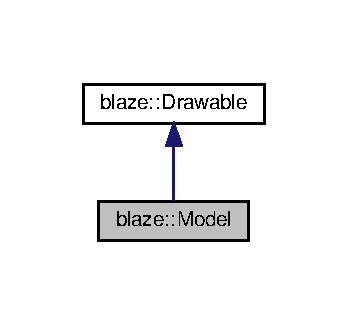
\includegraphics[width=167pt]{classblaze_1_1Model__inherit__graph}
\end{center}
\end{figure}


Collaboration diagram for blaze\+:\+:Model\+:\nopagebreak
\begin{figure}[H]
\begin{center}
\leavevmode
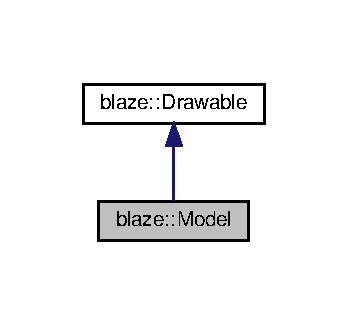
\includegraphics[width=167pt]{classblaze_1_1Model__coll__graph}
\end{center}
\end{figure}
\subsection*{Public Member Functions}
\begin{DoxyCompactItemize}
\item 
\mbox{\Hypertarget{classblaze_1_1Model_a0c8bd561406e0e56ef33c0072a7a48f6}\label{classblaze_1_1Model_a0c8bd561406e0e56ef33c0072a7a48f6}} 
\hyperlink{classblaze_1_1Model_a0c8bd561406e0e56ef33c0072a7a48f6}{Model} () noexcept
\begin{DoxyCompactList}\small\item\em Default constructor. \end{DoxyCompactList}\item 
\hyperlink{classblaze_1_1Model_a99429577ddc36a20a801f412f12d8b97}{Model} (const \hyperlink{classblaze_1_1Renderer}{Renderer} \&renderer, const std\+::vector$<$ int $>$ \&top\+\_\+level\+\_\+nodes, std\+::vector$<$ \hyperlink{structblaze_1_1Node}{Node} $>$ \&nodes, std\+::vector$<$ \hyperlink{structblaze_1_1Primitive}{Primitive} $>$ \&prims, std\+::vector$<$ \hyperlink{classblaze_1_1Material}{Material} $>$ \&mats, \hyperlink{classblaze_1_1IndexedVertexBuffer}{Indexed\+Vertex\+Buffer}$<$ \hyperlink{structblaze_1_1Vertex}{Vertex} $>$ \&\&ivb) noexcept
\begin{DoxyCompactList}\small\item\em Full constructor. \end{DoxyCompactList}\item 
\mbox{\Hypertarget{classblaze_1_1Model_a622eb89c06d2adbff32a65c9cf9ba6ce}\label{classblaze_1_1Model_a622eb89c06d2adbff32a65c9cf9ba6ce}} 
void \hyperlink{classblaze_1_1Model_a622eb89c06d2adbff32a65c9cf9ba6ce}{update} ()
\begin{DoxyCompactList}\small\item\em Update the transformation of the model starting from the root node. \end{DoxyCompactList}\end{DoxyCompactItemize}
\begin{Indent}\textbf{ Move Constructors.}\par
{\em For moving Models.

\hyperlink{classblaze_1_1Model}{Model} is a non copyable class. Copy constructors are deleted. }\begin{DoxyCompactItemize}
\item 
\mbox{\Hypertarget{classblaze_1_1Model_a96de780b11dc77a85707b34a2ab684c3}\label{classblaze_1_1Model_a96de780b11dc77a85707b34a2ab684c3}} 
{\bfseries Model} (\hyperlink{classblaze_1_1Model}{Model} \&\&other) noexcept
\item 
\mbox{\Hypertarget{classblaze_1_1Model_a45de45fd0522711e10029263f1194a6e}\label{classblaze_1_1Model_a45de45fd0522711e10029263f1194a6e}} 
\hyperlink{classblaze_1_1Model}{Model} \& {\bfseries operator=} (\hyperlink{classblaze_1_1Model}{Model} \&\&other) noexcept
\item 
\mbox{\Hypertarget{classblaze_1_1Model_a4d3cc8751c4fad2581f98b53fb15641f}\label{classblaze_1_1Model_a4d3cc8751c4fad2581f98b53fb15641f}} 
{\bfseries Model} (const \hyperlink{classblaze_1_1Model}{Model} \&other)=delete
\item 
\mbox{\Hypertarget{classblaze_1_1Model_ab7a55451c367564fde2c35190aa59b4d}\label{classblaze_1_1Model_ab7a55451c367564fde2c35190aa59b4d}} 
\hyperlink{classblaze_1_1Model}{Model} \& {\bfseries operator=} (const \hyperlink{classblaze_1_1Model}{Model} \&other)=delete
\end{DoxyCompactItemize}
\end{Indent}
\begin{Indent}\textbf{ Drawable Implementation}\par
{\em The implementation of the draw method from \hyperlink{classblaze_1_1Drawable}{Drawable} }\begin{DoxyCompactItemize}
\item 
void \hyperlink{classblaze_1_1Model_a00c3a74721bcad2d066de0c78313dae5}{draw} (Vk\+Command\+Buffer buf, Vk\+Pipeline\+Layout layout)
\begin{DoxyCompactList}\small\item\em Should draw the model with all the material and maps included. \end{DoxyCompactList}\item 
void \hyperlink{classblaze_1_1Model_ab5427d1b48ee3aedea9e405aa3892f5c}{draw\+Geometry} (Vk\+Command\+Buffer buf, Vk\+Pipeline\+Layout layout)
\begin{DoxyCompactList}\small\item\em Should draw only the geometry and not bind any materials. \end{DoxyCompactList}\end{DoxyCompactItemize}
\end{Indent}
\begin{Indent}\textbf{ Getters}\par
{\em Getters for the private members. }\begin{DoxyCompactItemize}
\item 
\mbox{\Hypertarget{classblaze_1_1Model_a46b15cb47420afca97d4b2b2cadb5755}\label{classblaze_1_1Model_a46b15cb47420afca97d4b2b2cadb5755}} 
\hyperlink{structblaze_1_1Node}{Node} $\ast$ {\bfseries get\+\_\+root} ()
\item 
\mbox{\Hypertarget{classblaze_1_1Model_a23100a15963328a52e55d5ff860316c1}\label{classblaze_1_1Model_a23100a15963328a52e55d5ff860316c1}} 
uint32\+\_\+t {\bfseries get\+\_\+vertex\+Count} () const
\item 
\mbox{\Hypertarget{classblaze_1_1Model_a1db46cfbc8cedf9e84a2ba8bd1a6ebe5}\label{classblaze_1_1Model_a1db46cfbc8cedf9e84a2ba8bd1a6ebe5}} 
uint32\+\_\+t {\bfseries get\+\_\+index\+Count} () const
\end{DoxyCompactItemize}
\end{Indent}


\subsection{Detailed Description}
Holds data from an entire gl\+TF 2.\+0 model. 

Contains the entire set of \hyperlink{classblaze_1_1Material}{Material}, \hyperlink{structblaze_1_1Primitive}{Primitive}, and \hyperlink{structblaze_1_1Node}{Node} as well the actual \hyperlink{classblaze_1_1IndexedVertexBuffer}{Indexed\+Vertex\+Buffer} and the root of the \hyperlink{structblaze_1_1Node}{Node} tree. 

\subsection{Constructor \& Destructor Documentation}
\mbox{\Hypertarget{classblaze_1_1Model_a99429577ddc36a20a801f412f12d8b97}\label{classblaze_1_1Model_a99429577ddc36a20a801f412f12d8b97}} 
\index{blaze\+::\+Model@{blaze\+::\+Model}!Model@{Model}}
\index{Model@{Model}!blaze\+::\+Model@{blaze\+::\+Model}}
\subsubsection{\texorpdfstring{Model()}{Model()}}
{\footnotesize\ttfamily blaze\+::\+Model\+::\+Model (\begin{DoxyParamCaption}\item[{const \hyperlink{classblaze_1_1Renderer}{Renderer} \&}]{renderer,  }\item[{const std\+::vector$<$ int $>$ \&}]{top\+\_\+level\+\_\+nodes,  }\item[{std\+::vector$<$ \hyperlink{structblaze_1_1Node}{Node} $>$ \&}]{nodes,  }\item[{std\+::vector$<$ \hyperlink{structblaze_1_1Primitive}{Primitive} $>$ \&}]{prims,  }\item[{std\+::vector$<$ \hyperlink{classblaze_1_1Material}{Material} $>$ \&}]{mats,  }\item[{\hyperlink{classblaze_1_1IndexedVertexBuffer}{Indexed\+Vertex\+Buffer}$<$ \hyperlink{structblaze_1_1Vertex}{Vertex} $>$ \&\&}]{ivb }\end{DoxyParamCaption})\hspace{0.3cm}{\ttfamily [noexcept]}}



Full constructor. 


\begin{DoxyParams}{Parameters}
{\em renderer} & The renderer used for the material. \\
\hline
{\em top\+\_\+level\+\_\+nodes} & The indices of nodes that are at the top level and have no parents. \\
\hline
{\em nodes} & The list of nodes in the model. \\
\hline
{\em prims} & The list of primitives in the model. \\
\hline
{\em mats} & The list of materials in the model. \\
\hline
{\em ivb} & The \hyperlink{classblaze_1_1IndexedVertexBuffer}{Indexed\+Vertex\+Buffer} that contains {\bfseries all} the vertices and indices. \\
\hline
\end{DoxyParams}


\subsection{Member Function Documentation}
\mbox{\Hypertarget{classblaze_1_1Model_a00c3a74721bcad2d066de0c78313dae5}\label{classblaze_1_1Model_a00c3a74721bcad2d066de0c78313dae5}} 
\index{blaze\+::\+Model@{blaze\+::\+Model}!draw@{draw}}
\index{draw@{draw}!blaze\+::\+Model@{blaze\+::\+Model}}
\subsubsection{\texorpdfstring{draw()}{draw()}}
{\footnotesize\ttfamily void blaze\+::\+Model\+::draw (\begin{DoxyParamCaption}\item[{Vk\+Command\+Buffer}]{cb,  }\item[{Vk\+Pipeline\+Layout}]{lay }\end{DoxyParamCaption})\hspace{0.3cm}{\ttfamily [virtual]}}



Should draw the model with all the material and maps included. 

This method is used during the primary render and should bind all the required buffers and textures and push material P\+CB.


\begin{DoxyParams}{Parameters}
{\em cb} & The command buffer to record to. \\
\hline
{\em lay} & The pipeline layout to bind descriptors. \\
\hline
\end{DoxyParams}


Implements \hyperlink{classblaze_1_1Drawable_a810b411ced93f27781a40a170714b590}{blaze\+::\+Drawable}.

\mbox{\Hypertarget{classblaze_1_1Model_ab5427d1b48ee3aedea9e405aa3892f5c}\label{classblaze_1_1Model_ab5427d1b48ee3aedea9e405aa3892f5c}} 
\index{blaze\+::\+Model@{blaze\+::\+Model}!draw\+Geometry@{draw\+Geometry}}
\index{draw\+Geometry@{draw\+Geometry}!blaze\+::\+Model@{blaze\+::\+Model}}
\subsubsection{\texorpdfstring{draw\+Geometry()}{drawGeometry()}}
{\footnotesize\ttfamily void blaze\+::\+Model\+::draw\+Geometry (\begin{DoxyParamCaption}\item[{Vk\+Command\+Buffer}]{cb,  }\item[{Vk\+Pipeline\+Layout}]{lay }\end{DoxyParamCaption})\hspace{0.3cm}{\ttfamily [virtual]}}



Should draw only the geometry and not bind any materials. 

This method is used for casting shadows and dowsn\textquotesingle{}t require any information beyond the position attribute of the \hyperlink{structblaze_1_1Vertex}{Vertex} and a model transformation P\+CB.


\begin{DoxyParams}{Parameters}
{\em cb} & The command buffer to record to. \\
\hline
{\em lay} & The pipeline layout to bind descriptors. \\
\hline
\end{DoxyParams}


Implements \hyperlink{classblaze_1_1Drawable_aa2bd171547027319e4254c47e0628163}{blaze\+::\+Drawable}.



The documentation for this class was generated from the following files\+:\begin{DoxyCompactItemize}
\item 
Blaze/drawables/Model.\+hpp\item 
Blaze/drawables/Model.\+cpp\end{DoxyCompactItemize}

\hypertarget{classblaze_1_1Model2}{}\section{blaze\+:\+:Model2 Class Reference}
\label{classblaze_1_1Model2}\index{blaze\+::\+Model2@{blaze\+::\+Model2}}


Inheritance diagram for blaze\+:\+:Model2\+:\nopagebreak
\begin{figure}[H]
\begin{center}
\leavevmode
\includegraphics[width=167pt]{classblaze_1_1Model2__inherit__graph}
\end{center}
\end{figure}


Collaboration diagram for blaze\+:\+:Model2\+:\nopagebreak
\begin{figure}[H]
\begin{center}
\leavevmode
\includegraphics[width=167pt]{classblaze_1_1Model2__coll__graph}
\end{center}
\end{figure}
\subsection*{Classes}
\begin{DoxyCompactItemize}
\item 
struct \hyperlink{structblaze_1_1Model2_1_1Material}{Material}
\end{DoxyCompactItemize}
\subsection*{Public Member Functions}
\begin{DoxyCompactItemize}
\item 
\mbox{\Hypertarget{classblaze_1_1Model2_a3122286acb99b24250c3ef919b0e3d9b}\label{classblaze_1_1Model2_a3122286acb99b24250c3ef919b0e3d9b}} 
\hyperlink{classblaze_1_1Model2_a3122286acb99b24250c3ef919b0e3d9b}{Model2} () noexcept
\begin{DoxyCompactList}\small\item\em Default constructor. \end{DoxyCompactList}\item 
\hyperlink{classblaze_1_1Model2_a1417c8c21b0003a068e20405f3b8e22c}{Model2} (const std\+::vector$<$ int $>$ \&top\+\_\+level\+\_\+nodes, std\+::vector$<$ \hyperlink{structblaze_1_1Node}{Node} $>$ \&\&nodes, std\+::vector$<$ \hyperlink{structblaze_1_1Primitive}{Primitive} $>$ \&\&prims, \hyperlink{classblaze_1_1IndexedVertexBuffer}{Indexed\+Vertex\+Buffer}$<$ \hyperlink{structblaze_1_1Vertex}{Vertex} $>$ \&\&ivb, \hyperlink{structblaze_1_1Model2_1_1Material}{Material} \&\&mat) noexcept
\begin{DoxyCompactList}\small\item\em Full constructor. \end{DoxyCompactList}\item 
\mbox{\Hypertarget{classblaze_1_1Model2_a05ebcffe0281b9cba1518fd9406e6911}\label{classblaze_1_1Model2_a05ebcffe0281b9cba1518fd9406e6911}} 
void \hyperlink{classblaze_1_1Model2_a05ebcffe0281b9cba1518fd9406e6911}{update} ()
\begin{DoxyCompactList}\small\item\em Update the transformation of the model starting from the root node. \end{DoxyCompactList}\end{DoxyCompactItemize}
\begin{Indent}\textbf{ Move Constructors.}\par
{\em For moving Models.

\hyperlink{classblaze_1_1Model}{Model} is a non copyable class. Copy constructors are deleted. }\begin{DoxyCompactItemize}
\item 
\mbox{\Hypertarget{classblaze_1_1Model2_a3483ac3041c9df6e6aae1482d7469f7e}\label{classblaze_1_1Model2_a3483ac3041c9df6e6aae1482d7469f7e}} 
{\bfseries Model2} (\hyperlink{classblaze_1_1Model2}{Model2} \&\&other)=delete
\item 
\mbox{\Hypertarget{classblaze_1_1Model2_a9cf8f52140f0e7e3214165bfc3ed1b30}\label{classblaze_1_1Model2_a9cf8f52140f0e7e3214165bfc3ed1b30}} 
\hyperlink{classblaze_1_1Model2}{Model2} \& {\bfseries operator=} (\hyperlink{classblaze_1_1Model2}{Model2} \&\&other)=delete
\item 
\mbox{\Hypertarget{classblaze_1_1Model2_af6f3dcda9570994cb0f6450e913e7fd3}\label{classblaze_1_1Model2_af6f3dcda9570994cb0f6450e913e7fd3}} 
{\bfseries Model2} (const \hyperlink{classblaze_1_1Model2}{Model2} \&other)=delete
\item 
\mbox{\Hypertarget{classblaze_1_1Model2_a07de3972eae0054bc18eb5eec76ee789}\label{classblaze_1_1Model2_a07de3972eae0054bc18eb5eec76ee789}} 
\hyperlink{classblaze_1_1Model2}{Model2} \& {\bfseries operator=} (const \hyperlink{classblaze_1_1Model2}{Model2} \&other)=delete
\end{DoxyCompactItemize}
\end{Indent}
\begin{Indent}\textbf{ Drawable Implementation}\par
{\em The implementation of the draw method from \hyperlink{classblaze_1_1Drawable}{Drawable} }\begin{DoxyCompactItemize}
\item 
void \hyperlink{classblaze_1_1Model2_a82bab7e2bed8bbbbff8f9c250785281d}{draw} (Vk\+Command\+Buffer buf, Vk\+Pipeline\+Layout layout) override
\begin{DoxyCompactList}\small\item\em Should draw the model with all the material and maps included. \end{DoxyCompactList}\item 
void \hyperlink{classblaze_1_1Model2_aadf59268e6faa861e27d6995a63552c3}{draw\+Geometry} (Vk\+Command\+Buffer buf, Vk\+Pipeline\+Layout layout) override
\begin{DoxyCompactList}\small\item\em Should draw only the geometry and not bind any materials. \end{DoxyCompactList}\end{DoxyCompactItemize}
\end{Indent}
\begin{Indent}\textbf{ Getters}\par
{\em Getters for the private members. }\begin{DoxyCompactItemize}
\item 
\mbox{\Hypertarget{classblaze_1_1Model2_aa1a25c9afa425bbab29f21f62406f4ee}\label{classblaze_1_1Model2_aa1a25c9afa425bbab29f21f62406f4ee}} 
\hyperlink{structblaze_1_1Node}{Node} $\ast$ {\bfseries get\+\_\+root} ()
\item 
\mbox{\Hypertarget{classblaze_1_1Model2_ac155ee39c93a29eb812eb34c08f0843a}\label{classblaze_1_1Model2_ac155ee39c93a29eb812eb34c08f0843a}} 
uint32\+\_\+t {\bfseries get\+\_\+vertex\+Count} () const
\item 
\mbox{\Hypertarget{classblaze_1_1Model2_a2de1c54d15f890a6054699aafc18dba6}\label{classblaze_1_1Model2_a2de1c54d15f890a6054699aafc18dba6}} 
uint32\+\_\+t {\bfseries get\+\_\+index\+Count} () const
\end{DoxyCompactItemize}
\end{Indent}


\subsection{Constructor \& Destructor Documentation}
\mbox{\Hypertarget{classblaze_1_1Model2_a1417c8c21b0003a068e20405f3b8e22c}\label{classblaze_1_1Model2_a1417c8c21b0003a068e20405f3b8e22c}} 
\index{blaze\+::\+Model2@{blaze\+::\+Model2}!Model2@{Model2}}
\index{Model2@{Model2}!blaze\+::\+Model2@{blaze\+::\+Model2}}
\subsubsection{\texorpdfstring{Model2()}{Model2()}}
{\footnotesize\ttfamily blaze\+::\+Model2\+::\+Model2 (\begin{DoxyParamCaption}\item[{const std\+::vector$<$ int $>$ \&}]{top\+\_\+level\+\_\+nodes,  }\item[{std\+::vector$<$ \hyperlink{structblaze_1_1Node}{Node} $>$ \&\&}]{nodes,  }\item[{std\+::vector$<$ \hyperlink{structblaze_1_1Primitive}{Primitive} $>$ \&\&}]{prims,  }\item[{\hyperlink{classblaze_1_1IndexedVertexBuffer}{Indexed\+Vertex\+Buffer}$<$ \hyperlink{structblaze_1_1Vertex}{Vertex} $>$ \&\&}]{ivb,  }\item[{\hyperlink{structblaze_1_1Model2_1_1Material}{Material} \&\&}]{mat }\end{DoxyParamCaption})\hspace{0.3cm}{\ttfamily [noexcept]}}



Full constructor. 


\begin{DoxyParams}{Parameters}
{\em top\+\_\+level\+\_\+nodes} & The indices of nodes that are at the top level and have no parents. \\
\hline
{\em nodes} & The list of nodes in the model. \\
\hline
{\em prims} & The list of primitives in the model. \\
\hline
{\em ivb} & The \hyperlink{classblaze_1_1IndexedVertexBuffer}{Indexed\+Vertex\+Buffer} that contains {\bfseries all} the vertices and indices. \\
\hline
{\em mat} & The material used in the model. \\
\hline
\end{DoxyParams}


\subsection{Member Function Documentation}
\mbox{\Hypertarget{classblaze_1_1Model2_a82bab7e2bed8bbbbff8f9c250785281d}\label{classblaze_1_1Model2_a82bab7e2bed8bbbbff8f9c250785281d}} 
\index{blaze\+::\+Model2@{blaze\+::\+Model2}!draw@{draw}}
\index{draw@{draw}!blaze\+::\+Model2@{blaze\+::\+Model2}}
\subsubsection{\texorpdfstring{draw()}{draw()}}
{\footnotesize\ttfamily void blaze\+::\+Model2\+::draw (\begin{DoxyParamCaption}\item[{Vk\+Command\+Buffer}]{cb,  }\item[{Vk\+Pipeline\+Layout}]{lay }\end{DoxyParamCaption})\hspace{0.3cm}{\ttfamily [override]}, {\ttfamily [virtual]}}



Should draw the model with all the material and maps included. 

This method is used during the primary render and should bind all the required buffers and textures and push material P\+CB.


\begin{DoxyParams}{Parameters}
{\em cb} & The command buffer to record to. \\
\hline
{\em lay} & The pipeline layout to bind descriptors. \\
\hline
\end{DoxyParams}


Implements \hyperlink{classblaze_1_1Drawable_a810b411ced93f27781a40a170714b590}{blaze\+::\+Drawable}.

\mbox{\Hypertarget{classblaze_1_1Model2_aadf59268e6faa861e27d6995a63552c3}\label{classblaze_1_1Model2_aadf59268e6faa861e27d6995a63552c3}} 
\index{blaze\+::\+Model2@{blaze\+::\+Model2}!draw\+Geometry@{draw\+Geometry}}
\index{draw\+Geometry@{draw\+Geometry}!blaze\+::\+Model2@{blaze\+::\+Model2}}
\subsubsection{\texorpdfstring{draw\+Geometry()}{drawGeometry()}}
{\footnotesize\ttfamily void blaze\+::\+Model2\+::draw\+Geometry (\begin{DoxyParamCaption}\item[{Vk\+Command\+Buffer}]{cb,  }\item[{Vk\+Pipeline\+Layout}]{lay }\end{DoxyParamCaption})\hspace{0.3cm}{\ttfamily [override]}, {\ttfamily [virtual]}}



Should draw only the geometry and not bind any materials. 

This method is used for casting shadows and dowsn\textquotesingle{}t require any information beyond the position attribute of the \hyperlink{structblaze_1_1Vertex}{Vertex} and a model transformation P\+CB.


\begin{DoxyParams}{Parameters}
{\em cb} & The command buffer to record to. \\
\hline
{\em lay} & The pipeline layout to bind descriptors. \\
\hline
\end{DoxyParams}


Implements \hyperlink{classblaze_1_1Drawable_aa2bd171547027319e4254c47e0628163}{blaze\+::\+Drawable}.



The documentation for this class was generated from the following files\+:\begin{DoxyCompactItemize}
\item 
Blaze/drawables/Model2.\+hpp\item 
Blaze/drawables/Model2.\+cpp\end{DoxyCompactItemize}

\hypertarget{classblaze_1_1ModelLoader}{}\section{blaze\+:\+:Model\+Loader Class Reference}
\label{classblaze_1_1ModelLoader}\index{blaze\+::\+Model\+Loader@{blaze\+::\+Model\+Loader}}
\subsection*{Public Member Functions}
\begin{DoxyCompactItemize}
\item 
\mbox{\Hypertarget{classblaze_1_1ModelLoader_ade1ecb4bcd2126ef731c2a0983bef260}\label{classblaze_1_1ModelLoader_ade1ecb4bcd2126ef731c2a0983bef260}} 
void {\bfseries scan} ()
\item 
\mbox{\Hypertarget{classblaze_1_1ModelLoader_a7f1b91186da558263a94f0843329411d}\label{classblaze_1_1ModelLoader_a7f1b91186da558263a94f0843329411d}} 
const std\+::vector$<$ std\+::string $>$ \& {\bfseries get\+File\+Names} () const
\item 
\mbox{\Hypertarget{classblaze_1_1ModelLoader_a970fb58b570aca28fd93ddca99f5bd2f}\label{classblaze_1_1ModelLoader_a970fb58b570aca28fd93ddca99f5bd2f}} 
std\+::shared\+\_\+ptr$<$ \hyperlink{classblaze_1_1Model2}{Model2} $>$ {\bfseries load\+Model} (const \hyperlink{classblaze_1_1Context}{Context} $\ast$context, const \hyperlink{structblaze_1_1spirv_1_1Shader}{spirv\+::\+Shader} \&shader, \hyperlink{structblaze_1_1spirv_1_1SetSingleton}{spirv\+::\+Set\+Singleton} \&\&set, uint32\+\_\+t idx)
\end{DoxyCompactItemize}


The documentation for this class was generated from the following files\+:\begin{DoxyCompactItemize}
\item 
Blaze/drawables/Model\+Loader.\+hpp\item 
Blaze/drawables/Model\+Loader.\+cpp\end{DoxyCompactItemize}

\hypertarget{structblaze_1_1ModelPushConstantBlock}{}\section{blaze\+:\+:Model\+Push\+Constant\+Block Struct Reference}
\label{structblaze_1_1ModelPushConstantBlock}\index{blaze\+::\+Model\+Push\+Constant\+Block@{blaze\+::\+Model\+Push\+Constant\+Block}}


P\+CB for sending \hyperlink{classblaze_1_1Model}{Model} matrix to the G\+PU.  




{\ttfamily \#include $<$Datatypes.\+hpp$>$}

\subsection*{Public Attributes}
\begin{DoxyCompactItemize}
\item 
\mbox{\Hypertarget{structblaze_1_1ModelPushConstantBlock_aea55d029bfaa5f7203c84ec0b181db42}\label{structblaze_1_1ModelPushConstantBlock_aea55d029bfaa5f7203c84ec0b181db42}} 
glm\+::mat4 {\bfseries model}
\end{DoxyCompactItemize}


\subsection{Detailed Description}
P\+CB for sending \hyperlink{classblaze_1_1Model}{Model} matrix to the G\+PU. 

The documentation for this struct was generated from the following file\+:\begin{DoxyCompactItemize}
\item 
Blaze/Datatypes.\+hpp\end{DoxyCompactItemize}

\hypertarget{structblaze_1_1Node}{}\section{blaze\+:\+:Node Struct Reference}
\label{structblaze_1_1Node}\index{blaze\+::\+Node@{blaze\+::\+Node}}


A node in the \hyperlink{classblaze_1_1Model}{Model} node tree.  




{\ttfamily \#include $<$Node.\+hpp$>$}



Collaboration diagram for blaze\+:\+:Node\+:\nopagebreak
\begin{figure}[H]
\begin{center}
\leavevmode
\includegraphics[width=214pt]{structblaze_1_1Node__coll__graph}
\end{center}
\end{figure}
\subsection*{Public Member Functions}
\begin{DoxyCompactItemize}
\item 
\hyperlink{structblaze_1_1Node_a80efd9604109b4b9ddbc72b462e35759}{Node} () noexcept
\begin{DoxyCompactList}\small\item\em Default constructor. \end{DoxyCompactList}\item 
\hyperlink{structblaze_1_1Node_a43d19db1208c11f1d2dd4195b699ab43}{Node} (const glm\+::vec3 \&trans, const glm\+::quat \&rot, const glm\+::vec3 \&sc, const std\+::vector$<$ int $>$ \&children, const std\+::pair$<$ int, int $>$ primitive\+\_\+range) noexcept
\begin{DoxyCompactList}\small\item\em Constructor that takes individual transform parameters. \end{DoxyCompactList}\item 
\hyperlink{structblaze_1_1Node_ae46aaa123fd42d14f915b7a656449862}{Node} (const glm\+::mat4 \&T\+RS, const std\+::vector$<$ int $>$ \&children, const std\+::pair$<$ int, int $>$ primitive\+\_\+range) noexcept
\begin{DoxyCompactList}\small\item\em Constructor that takes the entire T\+RS matrix. \end{DoxyCompactList}\item 
void \hyperlink{structblaze_1_1Node_aae2c0b30b1abb4b0314d2cabdbb867ed}{update} (const glm\+::mat4 parent\+T\+RS=glm\+::mat4(1.\+0f))
\begin{DoxyCompactList}\small\item\em Updates the World transform of the \hyperlink{structblaze_1_1Node}{Node}. \end{DoxyCompactList}\end{DoxyCompactItemize}
\begin{Indent}\textbf{ Move Constructors}\par
{\em For moving a \hyperlink{structblaze_1_1Node}{Node}.

Nodes are not copyable. Hance copy constructors are deleted. }\begin{DoxyCompactItemize}
\item 
\mbox{\Hypertarget{structblaze_1_1Node_aaae7412f72b9c55374a75b6488186725}\label{structblaze_1_1Node_aaae7412f72b9c55374a75b6488186725}} 
{\bfseries Node} (\hyperlink{structblaze_1_1Node}{Node} \&\&other) noexcept
\item 
\mbox{\Hypertarget{structblaze_1_1Node_abb0f200b8c985f10bd4ff2956154ef9b}\label{structblaze_1_1Node_abb0f200b8c985f10bd4ff2956154ef9b}} 
\hyperlink{structblaze_1_1Node}{Node} \& {\bfseries operator=} (\hyperlink{structblaze_1_1Node}{Node} \&\&other) noexcept
\item 
\mbox{\Hypertarget{structblaze_1_1Node_ad1a0fafd4be3301fddf0a434a2f2ba12}\label{structblaze_1_1Node_ad1a0fafd4be3301fddf0a434a2f2ba12}} 
{\bfseries Node} (const \hyperlink{structblaze_1_1Node}{Node} \&other)=delete
\item 
\mbox{\Hypertarget{structblaze_1_1Node_a64d32e746903bb69d8c59fa7518974ce}\label{structblaze_1_1Node_a64d32e746903bb69d8c59fa7518974ce}} 
\hyperlink{structblaze_1_1Node}{Node} \& {\bfseries operator=} (const \hyperlink{structblaze_1_1Node}{Node} \&other)=delete
\end{DoxyCompactItemize}
\end{Indent}
\subsection*{Public Attributes}
\begin{DoxyCompactItemize}
\item 
\mbox{\Hypertarget{structblaze_1_1Node_a9f0981eeb9569f9135a7604c7d13fb52}\label{structblaze_1_1Node_a9f0981eeb9569f9135a7604c7d13fb52}} 
glm\+::vec3 {\bfseries translation}
\item 
\mbox{\Hypertarget{structblaze_1_1Node_a6fb776faf88ea9ab605acf79975ebc11}\label{structblaze_1_1Node_a6fb776faf88ea9ab605acf79975ebc11}} 
glm\+::quat {\bfseries rotation}
\item 
\mbox{\Hypertarget{structblaze_1_1Node_a59018efc4c257991ad1bcabf6087d078}\label{structblaze_1_1Node_a59018efc4c257991ad1bcabf6087d078}} 
glm\+::vec3 {\bfseries scale}
\item 
\mbox{\Hypertarget{structblaze_1_1Node_a96a4d837006cdc49e802a85b77e4fb67}\label{structblaze_1_1Node_a96a4d837006cdc49e802a85b77e4fb67}} 
glm\+::mat4 {\bfseries local\+T\+RS}
\item 
\mbox{\Hypertarget{structblaze_1_1Node_ab4e58da330ba682cec0425fe72c1f8b5}\label{structblaze_1_1Node_ab4e58da330ba682cec0425fe72c1f8b5}} 
\hyperlink{structblaze_1_1ModelPushConstantBlock}{Model\+Push\+Constant\+Block} {\bfseries pcb}
\item 
\mbox{\Hypertarget{structblaze_1_1Node_a84ae34bec74601d72c09c45eea4f8133}\label{structblaze_1_1Node_a84ae34bec74601d72c09c45eea4f8133}} 
std\+::vector$<$ int $>$ {\bfseries children}
\item 
\mbox{\Hypertarget{structblaze_1_1Node_acbdbbfc2dd74227b1154844c200a462a}\label{structblaze_1_1Node_acbdbbfc2dd74227b1154844c200a462a}} 
std\+::pair$<$ int, int $>$ {\bfseries primitive\+\_\+range}
\end{DoxyCompactItemize}


\subsection{Detailed Description}
A node in the \hyperlink{classblaze_1_1Model}{Model} node tree. 

Each node contains a model transformation that applies to all primitives in the node, as well as the children of the node.

Each node must have atleast one child or one primitive under it. 

\subsection{Constructor \& Destructor Documentation}
\mbox{\Hypertarget{structblaze_1_1Node_a80efd9604109b4b9ddbc72b462e35759}\label{structblaze_1_1Node_a80efd9604109b4b9ddbc72b462e35759}} 
\index{blaze\+::\+Node@{blaze\+::\+Node}!Node@{Node}}
\index{Node@{Node}!blaze\+::\+Node@{blaze\+::\+Node}}
\subsubsection{\texorpdfstring{Node()}{Node()}\hspace{0.1cm}{\footnotesize\ttfamily [1/3]}}
{\footnotesize\ttfamily blaze\+::\+Node\+::\+Node (\begin{DoxyParamCaption}{ }\end{DoxyParamCaption})\hspace{0.3cm}{\ttfamily [noexcept]}}



Default constructor. 

The default constructor of the \hyperlink{structblaze_1_1Node}{Node}. Every value is set to their default. \mbox{\Hypertarget{structblaze_1_1Node_a43d19db1208c11f1d2dd4195b699ab43}\label{structblaze_1_1Node_a43d19db1208c11f1d2dd4195b699ab43}} 
\index{blaze\+::\+Node@{blaze\+::\+Node}!Node@{Node}}
\index{Node@{Node}!blaze\+::\+Node@{blaze\+::\+Node}}
\subsubsection{\texorpdfstring{Node()}{Node()}\hspace{0.1cm}{\footnotesize\ttfamily [2/3]}}
{\footnotesize\ttfamily blaze\+::\+Node\+::\+Node (\begin{DoxyParamCaption}\item[{const glm\+::vec3 \&}]{trans,  }\item[{const glm\+::quat \&}]{rot,  }\item[{const glm\+::vec3 \&}]{sc,  }\item[{const std\+::vector$<$ int $>$ \&}]{children,  }\item[{const std\+::pair$<$ int, int $>$}]{primitive\+\_\+range }\end{DoxyParamCaption})\hspace{0.3cm}{\ttfamily [noexcept]}}



Constructor that takes individual transform parameters. 


\begin{DoxyParams}{Parameters}
{\em trans} & Translation \\
\hline
{\em rot} & Rotation \\
\hline
{\em sc} & Scale \\
\hline
{\em children} & Indices of the children of the node in the \hyperlink{classblaze_1_1Model}{Model}. \\
\hline
{\em primitive\+\_\+range} & The range of indices of primitives under this \hyperlink{structblaze_1_1Node}{Node}. \\
\hline
\end{DoxyParams}
\mbox{\Hypertarget{structblaze_1_1Node_ae46aaa123fd42d14f915b7a656449862}\label{structblaze_1_1Node_ae46aaa123fd42d14f915b7a656449862}} 
\index{blaze\+::\+Node@{blaze\+::\+Node}!Node@{Node}}
\index{Node@{Node}!blaze\+::\+Node@{blaze\+::\+Node}}
\subsubsection{\texorpdfstring{Node()}{Node()}\hspace{0.1cm}{\footnotesize\ttfamily [3/3]}}
{\footnotesize\ttfamily blaze\+::\+Node\+::\+Node (\begin{DoxyParamCaption}\item[{const glm\+::mat4 \&}]{T\+RS,  }\item[{const std\+::vector$<$ int $>$ \&}]{children,  }\item[{const std\+::pair$<$ int, int $>$}]{primitive\+\_\+range }\end{DoxyParamCaption})\hspace{0.3cm}{\ttfamily [noexcept]}}



Constructor that takes the entire T\+RS matrix. 


\begin{DoxyParams}{Parameters}
{\em T\+RS} & Translation Rotation Scale matrix \\
\hline
{\em children} & Indices of the children of the node in the \hyperlink{classblaze_1_1Model}{Model}. \\
\hline
{\em primitive\+\_\+range} & The range of indices of primitives under this \hyperlink{structblaze_1_1Node}{Node}. \\
\hline
\end{DoxyParams}


\subsection{Member Function Documentation}
\mbox{\Hypertarget{structblaze_1_1Node_aae2c0b30b1abb4b0314d2cabdbb867ed}\label{structblaze_1_1Node_aae2c0b30b1abb4b0314d2cabdbb867ed}} 
\index{blaze\+::\+Node@{blaze\+::\+Node}!update@{update}}
\index{update@{update}!blaze\+::\+Node@{blaze\+::\+Node}}
\subsubsection{\texorpdfstring{update()}{update()}}
{\footnotesize\ttfamily blaze\+::\+Node\+::update (\begin{DoxyParamCaption}\item[{const glm\+::mat4}]{parent\+T\+RS = {\ttfamily glm\+:\+:mat4(1.0f)} }\end{DoxyParamCaption})}



Updates the World transform of the \hyperlink{structblaze_1_1Node}{Node}. 

Updates the local transform according to changes in the three components. Updates the world transform according to local transform and parent transform.


\begin{DoxyParams}{Parameters}
{\em parent\+T\+RS} & Parent transform. \\
\hline
\end{DoxyParams}


The documentation for this struct was generated from the following files\+:\begin{DoxyCompactItemize}
\item 
Blaze/drawables/Node.\+hpp\item 
Blaze/drawables/Node.\+cpp\end{DoxyCompactItemize}

\hypertarget{classblaze_1_1util_1_1PackedHandler}{}\section{blaze\+:\+:util\+:\+:Packed\+Handler$<$ T $>$ Class Template Reference}
\label{classblaze_1_1util_1_1PackedHandler}\index{blaze\+::util\+::\+Packed\+Handler$<$ T $>$@{blaze\+::util\+::\+Packed\+Handler$<$ T $>$}}
\subsection*{Public Types}
\begin{DoxyCompactItemize}
\item 
\mbox{\Hypertarget{classblaze_1_1util_1_1PackedHandler_aa14ddb733eb2fb3fceeb8c2a7899ab18}\label{classblaze_1_1util_1_1PackedHandler_aa14ddb733eb2fb3fceeb8c2a7899ab18}} 
using {\bfseries Handle} = Outer\+Handle
\end{DoxyCompactItemize}
\subsection*{Public Member Functions}
\begin{DoxyCompactItemize}
\item 
\mbox{\Hypertarget{classblaze_1_1util_1_1PackedHandler_a6bdbedd66950ab4693b1558d3a159ca6}\label{classblaze_1_1util_1_1PackedHandler_a6bdbedd66950ab4693b1558d3a159ca6}} 
Handle {\bfseries add} (T \&\&val)
\item 
\mbox{\Hypertarget{classblaze_1_1util_1_1PackedHandler_a071593822b585108135246147ba5e09b}\label{classblaze_1_1util_1_1PackedHandler_a071593822b585108135246147ba5e09b}} 
Handle {\bfseries add} (const T \&val)
\item 
\mbox{\Hypertarget{classblaze_1_1util_1_1PackedHandler_a33b1e035cc41c8d9c7be6a0dd2d0b5be}\label{classblaze_1_1util_1_1PackedHandler_a33b1e035cc41c8d9c7be6a0dd2d0b5be}} 
auto {\bfseries begin} () const
\item 
\mbox{\Hypertarget{classblaze_1_1util_1_1PackedHandler_a903887e5159c7543cc0aa65fc8a171a5}\label{classblaze_1_1util_1_1PackedHandler_a903887e5159c7543cc0aa65fc8a171a5}} 
auto {\bfseries end} () const
\item 
\mbox{\Hypertarget{classblaze_1_1util_1_1PackedHandler_a0b20397d35d371fa980698eda777be93}\label{classblaze_1_1util_1_1PackedHandler_a0b20397d35d371fa980698eda777be93}} 
const std\+::vector$<$ T $>$ \& {\bfseries get\+\_\+data} ()
\end{DoxyCompactItemize}


The documentation for this class was generated from the following file\+:\begin{DoxyCompactItemize}
\item 
Blaze/util/Packed\+Handler.\+hpp\end{DoxyCompactItemize}

\hypertarget{structblaze_1_1Model2_1_1Material_1_1PCB}{}\section{blaze\+:\+:Model2\+:\+:Material\+:\+:P\+CB Struct Reference}
\label{structblaze_1_1Model2_1_1Material_1_1PCB}\index{blaze\+::\+Model2\+::\+Material\+::\+P\+CB@{blaze\+::\+Model2\+::\+Material\+::\+P\+CB}}
\subsection*{Public Attributes}
\begin{DoxyCompactItemize}
\item 
\mbox{\Hypertarget{structblaze_1_1Model2_1_1Material_1_1PCB_a186d93254630e3011ccb4987ebfb074d}\label{structblaze_1_1Model2_1_1Material_1_1PCB_a186d93254630e3011ccb4987ebfb074d}} 
glm\+::vec4 {\bfseries base\+Color\+Factor} \{1.\+0f, 0, 1.\+0f, 1.\+0f\}
\item 
\mbox{\Hypertarget{structblaze_1_1Model2_1_1Material_1_1PCB_a6bd961d60bfe0c8c9cfbf5888eb6a8b8}\label{structblaze_1_1Model2_1_1Material_1_1PCB_a6bd961d60bfe0c8c9cfbf5888eb6a8b8}} 
glm\+::vec4 {\bfseries emissive\+Color\+Factor} \{1.\+0f, 0, 1.\+0f, 1.\+0f\}
\item 
\mbox{\Hypertarget{structblaze_1_1Model2_1_1Material_1_1PCB_a0bbda278a47afbc97eb454af9e3b75f6}\label{structblaze_1_1Model2_1_1Material_1_1PCB_a0bbda278a47afbc97eb454af9e3b75f6}} 
float {\bfseries metallic\+Factor} \{1.\+0f\}
\item 
\mbox{\Hypertarget{structblaze_1_1Model2_1_1Material_1_1PCB_a24720893df9feeed709b41547a2c44f4}\label{structblaze_1_1Model2_1_1Material_1_1PCB_a24720893df9feeed709b41547a2c44f4}} 
float {\bfseries roughness\+Factor} \{1.\+0f\}
\item 
\mbox{\Hypertarget{structblaze_1_1Model2_1_1Material_1_1PCB_a3c17f4812b264504a1082940704fd869}\label{structblaze_1_1Model2_1_1Material_1_1PCB_a3c17f4812b264504a1082940704fd869}} 
int {\bfseries base\+Color\+Texture\+Set} \{-\/1\}
\item 
\mbox{\Hypertarget{structblaze_1_1Model2_1_1Material_1_1PCB_ae9482f007ac0b2ddbbcc6bf6e7e10c1e}\label{structblaze_1_1Model2_1_1Material_1_1PCB_ae9482f007ac0b2ddbbcc6bf6e7e10c1e}} 
int {\bfseries physical\+Descriptor\+Texture\+Set} \{-\/1\}
\item 
\mbox{\Hypertarget{structblaze_1_1Model2_1_1Material_1_1PCB_a84c33c1d140a4a60001be3a08fce22f4}\label{structblaze_1_1Model2_1_1Material_1_1PCB_a84c33c1d140a4a60001be3a08fce22f4}} 
int {\bfseries normal\+Texture\+Set} \{-\/1\}
\item 
\mbox{\Hypertarget{structblaze_1_1Model2_1_1Material_1_1PCB_ab8efe1a0b2ecb017eb64a615d667b434}\label{structblaze_1_1Model2_1_1Material_1_1PCB_ab8efe1a0b2ecb017eb64a615d667b434}} 
int {\bfseries occlusion\+Texture\+Set} \{-\/1\}
\item 
\mbox{\Hypertarget{structblaze_1_1Model2_1_1Material_1_1PCB_af074678bee79b546f03e74dc75d8d873}\label{structblaze_1_1Model2_1_1Material_1_1PCB_af074678bee79b546f03e74dc75d8d873}} 
int {\bfseries emissive\+Texture\+Set} \{-\/1\}
\item 
\mbox{\Hypertarget{structblaze_1_1Model2_1_1Material_1_1PCB_a19d91fe0c1a9bf12642b134a2d21b7cf}\label{structblaze_1_1Model2_1_1Material_1_1PCB_a19d91fe0c1a9bf12642b134a2d21b7cf}} 
int {\bfseries texture\+Arr\+Idx} \{0\}
\end{DoxyCompactItemize}


The documentation for this struct was generated from the following file\+:\begin{DoxyCompactItemize}
\item 
Blaze/drawables/Model2.\+hpp\end{DoxyCompactItemize}

\hypertarget{structblaze_1_1spirv_1_1Pipeline}{}\section{blaze\+:\+:spirv\+:\+:Pipeline Struct Reference}
\label{structblaze_1_1spirv_1_1Pipeline}\index{blaze\+::spirv\+::\+Pipeline@{blaze\+::spirv\+::\+Pipeline}}
\subsection*{Public Member Functions}
\begin{DoxyCompactItemize}
\item 
\mbox{\Hypertarget{structblaze_1_1spirv_1_1Pipeline_a29a57d4ce3b934d5f23398eab5609cf7}\label{structblaze_1_1spirv_1_1Pipeline_a29a57d4ce3b934d5f23398eab5609cf7}} 
void {\bfseries bind} (Vk\+Command\+Buffer cmdbuf)
\end{DoxyCompactItemize}
\subsection*{Public Attributes}
\begin{DoxyCompactItemize}
\item 
\mbox{\Hypertarget{structblaze_1_1spirv_1_1Pipeline_a013ec27941075de8125c23e142ab4931}\label{structblaze_1_1spirv_1_1Pipeline_a013ec27941075de8125c23e142ab4931}} 
vkw\+::\+Pipeline {\bfseries pipeline}
\item 
\mbox{\Hypertarget{structblaze_1_1spirv_1_1Pipeline_a71832ee550924d6b1bb0e10ea8bd817c}\label{structblaze_1_1spirv_1_1Pipeline_a71832ee550924d6b1bb0e10ea8bd817c}} 
Vk\+Pipeline\+Bind\+Point {\bfseries bind\+Point}
\end{DoxyCompactItemize}


The documentation for this struct was generated from the following file\+:\begin{DoxyCompactItemize}
\item 
Blaze/spirv/Pipeline.\+hpp\end{DoxyCompactItemize}

\hypertarget{classblaze_1_1spirv_1_1PipelineFactory}{}\section{blaze\+:\+:spirv\+:\+:Pipeline\+Factory Class Reference}
\label{classblaze_1_1spirv_1_1PipelineFactory}\index{blaze\+::spirv\+::\+Pipeline\+Factory@{blaze\+::spirv\+::\+Pipeline\+Factory}}
\subsection*{Public Member Functions}
\begin{DoxyCompactItemize}
\item 
\mbox{\Hypertarget{classblaze_1_1spirv_1_1PipelineFactory_acdb4e699d0cb4898a4fa51e0b7e14e70}\label{classblaze_1_1spirv_1_1PipelineFactory_acdb4e699d0cb4898a4fa51e0b7e14e70}} 
{\bfseries Pipeline\+Factory} (Vk\+Device device) noexcept
\item 
\mbox{\Hypertarget{classblaze_1_1spirv_1_1PipelineFactory_ac1b6b95ed9659c501ecb4ac626a2e1bb}\label{classblaze_1_1spirv_1_1PipelineFactory_ac1b6b95ed9659c501ecb4ac626a2e1bb}} 
\hyperlink{structblaze_1_1spirv_1_1Shader}{Shader} {\bfseries create\+Shader} (const std\+::vector$<$ \hyperlink{structblaze_1_1spirv_1_1ShaderStageData}{Shader\+Stage\+Data} $>$ \&stages)
\item 
\mbox{\Hypertarget{classblaze_1_1spirv_1_1PipelineFactory_a46ebc6903dfacabb5c27146762979f14}\label{classblaze_1_1spirv_1_1PipelineFactory_a46ebc6903dfacabb5c27146762979f14}} 
\hyperlink{structblaze_1_1spirv_1_1Pipeline}{Pipeline} {\bfseries create\+Graphics\+Pipeline} (const \hyperlink{structblaze_1_1spirv_1_1Shader}{Shader} \&shader, const \hyperlink{structblaze_1_1spirv_1_1RenderPass}{Render\+Pass} \&render\+Pass, const \hyperlink{structblaze_1_1spirv_1_1GraphicsPipelineCreateInfo}{Graphics\+Pipeline\+Create\+Info} \&create\+Info)
\item 
\mbox{\Hypertarget{classblaze_1_1spirv_1_1PipelineFactory_ab4db0891a3c6ae0419cdf2df2fc0fd60}\label{classblaze_1_1spirv_1_1PipelineFactory_ab4db0891a3c6ae0419cdf2df2fc0fd60}} 
\hyperlink{structblaze_1_1spirv_1_1RenderPass}{Render\+Pass} {\bfseries create\+Render\+Pass} (const std\+::vector$<$ \hyperlink{structblaze_1_1spirv_1_1AttachmentFormat}{Attachment\+Format} $>$ \&formats, const std\+::vector$<$ Vk\+Subpass\+Description $>$ \&subpasses, \hyperlink{structblaze_1_1spirv_1_1LoadStoreConfig}{Load\+Store\+Config} config, const Vk\+Render\+Pass\+Multiview\+Create\+Info $\ast$multiview=nullptr)
\item 
\mbox{\Hypertarget{classblaze_1_1spirv_1_1PipelineFactory_ab7e18c33bc6970c3a766165a52b0d564}\label{classblaze_1_1spirv_1_1PipelineFactory_ab7e18c33bc6970c3a766165a52b0d564}} 
\hyperlink{structblaze_1_1spirv_1_1SetVector}{Set\+Vector} {\bfseries create\+Sets} (const \hyperlink{structblaze_1_1spirv_1_1Shader_1_1Set}{Shader\+::\+Set} \&set, uint32\+\_\+t count)
\item 
\mbox{\Hypertarget{classblaze_1_1spirv_1_1PipelineFactory_ab2a6b51346548c45e1f6b967d7322f37}\label{classblaze_1_1spirv_1_1PipelineFactory_ab2a6b51346548c45e1f6b967d7322f37}} 
\hyperlink{structblaze_1_1spirv_1_1SetSingleton}{Set\+Singleton} {\bfseries create\+Set} (const \hyperlink{structblaze_1_1spirv_1_1Shader_1_1Set}{Shader\+::\+Set} \&set)
\item 
\mbox{\Hypertarget{classblaze_1_1spirv_1_1PipelineFactory_a24dd894f334060f3703f81928c466e8b}\label{classblaze_1_1spirv_1_1PipelineFactory_a24dd894f334060f3703f81928c466e8b}} 
bool {\bfseries valid} () const
\end{DoxyCompactItemize}


The documentation for this class was generated from the following files\+:\begin{DoxyCompactItemize}
\item 
Blaze/spirv/Pipeline\+Factory.\+hpp\item 
Blaze/spirv/Pipeline\+Factory.\+cpp\end{DoxyCompactItemize}

\hypertarget{classPointShadow}{}\section{Point\+Shadow Class Reference}
\label{classPointShadow}\index{Point\+Shadow@{Point\+Shadow}}


Encapsulates the attachments and framebuffer for a point light shadow.  




{\ttfamily \#include $<$Light\+System.\+hpp$>$}



\subsection{Detailed Description}
Encapsulates the attachments and framebuffer for a point light shadow. 

Contains the shadow\+Map (R32) and a depth\+Map (D32) along with the framebuffer and viewport configured.

\begin{DoxyNote}{Note}
Not supposed to be used externally. 
\end{DoxyNote}


The documentation for this class was generated from the following file\+:\begin{DoxyCompactItemize}
\item 
Blaze/Light\+System.\+hpp\end{DoxyCompactItemize}

\hypertarget{structblaze_1_1Primitive}{}\section{blaze\+:\+:Primitive Struct Reference}
\label{structblaze_1_1Primitive}\index{blaze\+::\+Primitive@{blaze\+::\+Primitive}}


Denotes the data of a single primitive.  




{\ttfamily \#include $<$Node.\+hpp$>$}

\subsection*{Public Member Functions}
\begin{DoxyCompactItemize}
\item 
\mbox{\Hypertarget{structblaze_1_1Primitive_ad0b907c09e78d280f97510cfd36b684a}\label{structblaze_1_1Primitive_ad0b907c09e78d280f97510cfd36b684a}} 
\hyperlink{structblaze_1_1Primitive_ad0b907c09e78d280f97510cfd36b684a}{Primitive} (uint32\+\_\+t first\+Index, uint32\+\_\+t vertex\+Count, uint32\+\_\+t index\+Count, uint32\+\_\+t material)
\begin{DoxyCompactList}\small\item\em Constructor. \end{DoxyCompactList}\end{DoxyCompactItemize}
\subsection*{Public Attributes}
\begin{DoxyCompactItemize}
\item 
\mbox{\Hypertarget{structblaze_1_1Primitive_a780342ae3a6facb806cf9786c7b884d2}\label{structblaze_1_1Primitive_a780342ae3a6facb806cf9786c7b884d2}} 
uint32\+\_\+t {\bfseries first\+Index}
\item 
\mbox{\Hypertarget{structblaze_1_1Primitive_a9b10c1b154e42010399c5dc10b08fc5a}\label{structblaze_1_1Primitive_a9b10c1b154e42010399c5dc10b08fc5a}} 
uint32\+\_\+t {\bfseries vertex\+Count}
\item 
\mbox{\Hypertarget{structblaze_1_1Primitive_a7b85b53fa0c97a37ac71d2f625681644}\label{structblaze_1_1Primitive_a7b85b53fa0c97a37ac71d2f625681644}} 
uint32\+\_\+t {\bfseries index\+Count}
\item 
\mbox{\Hypertarget{structblaze_1_1Primitive_ad22171261ecd5aeca5007d1f4fea3a8c}\label{structblaze_1_1Primitive_ad22171261ecd5aeca5007d1f4fea3a8c}} 
uint32\+\_\+t {\bfseries material}
\item 
\mbox{\Hypertarget{structblaze_1_1Primitive_a5c406e99653f5b6fa3f4a7bee5946133}\label{structblaze_1_1Primitive_a5c406e99653f5b6fa3f4a7bee5946133}} 
bool {\bfseries has\+Index}
\end{DoxyCompactItemize}


\subsection{Detailed Description}
Denotes the data of a single primitive. 

The class is used for a singular mesh in a \hyperlink{structblaze_1_1Node}{Node} that is constructed out of a set of vertices that are kept separately.

Each primitive can have its own vertices and material, or can share with other primitives in the \hyperlink{classblaze_1_1Model}{Model} 

The documentation for this struct was generated from the following file\+:\begin{DoxyCompactItemize}
\item 
Blaze/drawables/Node.\+hpp\end{DoxyCompactItemize}

\hypertarget{classblaze_1_1util_1_1Process}{}\section{blaze\+:\+:util\+:\+:Process$<$ P\+CB $>$ Class Template Reference}
\label{classblaze_1_1util_1_1Process}\index{blaze\+::util\+::\+Process$<$ P\+C\+B $>$@{blaze\+::util\+::\+Process$<$ P\+C\+B $>$}}


The static processing class for converting from a descriptor to a cubemap.  




{\ttfamily \#include $<$processing.\+hpp$>$}

\subsection*{Static Public Member Functions}
\begin{DoxyCompactItemize}
\item 
static \hyperlink{classblaze_1_1TextureCube}{Texture\+Cube} \hyperlink{classblaze_1_1util_1_1Process_a56e7bdeca0b7e0af8b8ace326c63d46e}{convert\+Descriptor\+To\+Cubemap} (const \hyperlink{classblaze_1_1Context}{Context} $\ast$context, const \hyperlink{structblaze_1_1util_1_1Texture2CubemapInfo}{Texture2\+Cubemap\+Info}$<$ P\+CB $>$ \&info)
\begin{DoxyCompactList}\small\item\em Converts the descriptor to a cubemap. \end{DoxyCompactList}\end{DoxyCompactItemize}


\subsection{Detailed Description}
\subsubsection*{template$<$typename P\+CB$>$\newline
class blaze\+::util\+::\+Process$<$ P\+C\+B $>$}

The static processing class for converting from a descriptor to a cubemap. 


\begin{DoxyTemplParams}{Template Parameters}
{\em P\+CB} & The type of the struct used for P\+CB. \\
\hline
\end{DoxyTemplParams}


\subsection{Member Function Documentation}
\mbox{\Hypertarget{classblaze_1_1util_1_1Process_a56e7bdeca0b7e0af8b8ace326c63d46e}\label{classblaze_1_1util_1_1Process_a56e7bdeca0b7e0af8b8ace326c63d46e}} 
\index{blaze\+::util\+::\+Process@{blaze\+::util\+::\+Process}!convert\+Descriptor\+To\+Cubemap@{convert\+Descriptor\+To\+Cubemap}}
\index{convert\+Descriptor\+To\+Cubemap@{convert\+Descriptor\+To\+Cubemap}!blaze\+::util\+::\+Process@{blaze\+::util\+::\+Process}}
\subsubsection{\texorpdfstring{convert\+Descriptor\+To\+Cubemap()}{convertDescriptorToCubemap()}}
{\footnotesize\ttfamily template$<$typename P\+CB $>$ \\
static \hyperlink{classblaze_1_1TextureCube}{Texture\+Cube} \hyperlink{classblaze_1_1util_1_1Process}{blaze\+::util\+::\+Process}$<$ P\+CB $>$\+::convert\+Descriptor\+To\+Cubemap (\begin{DoxyParamCaption}\item[{const \hyperlink{classblaze_1_1Context}{Context} $\ast$}]{context,  }\item[{const \hyperlink{structblaze_1_1util_1_1Texture2CubemapInfo}{Texture2\+Cubemap\+Info}$<$ P\+CB $>$ \&}]{info }\end{DoxyParamCaption})\hspace{0.3cm}{\ttfamily [inline]}, {\ttfamily [static]}}



Converts the descriptor to a cubemap. 


\begin{DoxyParams}{Parameters}
{\em context} & The current Vulkan \hyperlink{classblaze_1_1Context}{Context}. \\
\hline
{\em info} & The \hyperlink{structblaze_1_1util_1_1Texture2CubemapInfo}{Texture2\+Cubemap\+Info} to configure the type. \\
\hline
\end{DoxyParams}


The documentation for this class was generated from the following file\+:\begin{DoxyCompactItemize}
\item 
Blaze/util/processing.\+hpp\end{DoxyCompactItemize}

\hypertarget{structblaze_1_1spirv_1_1Shader_1_1PushConstant}{}\section{blaze\+:\+:spirv\+:\+:Shader\+:\+:Push\+Constant Struct Reference}
\label{structblaze_1_1spirv_1_1Shader_1_1PushConstant}\index{blaze\+::spirv\+::\+Shader\+::\+Push\+Constant@{blaze\+::spirv\+::\+Shader\+::\+Push\+Constant}}
\subsection*{Public Attributes}
\begin{DoxyCompactItemize}
\item 
\mbox{\Hypertarget{structblaze_1_1spirv_1_1Shader_1_1PushConstant_a402407530e6343b10f4f044907b16ce6}\label{structblaze_1_1spirv_1_1Shader_1_1PushConstant_a402407530e6343b10f4f044907b16ce6}} 
uint32\+\_\+t {\bfseries size} = 0
\item 
\mbox{\Hypertarget{structblaze_1_1spirv_1_1Shader_1_1PushConstant_a365b9dcfad25720275ca8841f77de389}\label{structblaze_1_1spirv_1_1Shader_1_1PushConstant_a365b9dcfad25720275ca8841f77de389}} 
uint32\+\_\+t {\bfseries stage} = 0
\end{DoxyCompactItemize}


The documentation for this struct was generated from the following file\+:\begin{DoxyCompactItemize}
\item 
Blaze/spirv/Pipeline.\+hpp\end{DoxyCompactItemize}

\hypertarget{structblaze_1_1util_1_1QueueFamilyIndices}{}\section{blaze\+:\+:util\+:\+:Queue\+Family\+Indices Struct Reference}
\label{structblaze_1_1util_1_1QueueFamilyIndices}\index{blaze\+::util\+::\+Queue\+Family\+Indices@{blaze\+::util\+::\+Queue\+Family\+Indices}}


Holds the indices for the queue families to use in the context.  




{\ttfamily \#include $<$Device\+Selection.\+hpp$>$}

\subsection*{Public Member Functions}
\begin{DoxyCompactItemize}
\item 
bool \hyperlink{structblaze_1_1util_1_1QueueFamilyIndices_a23bf708816aa6ff4e554610003056885}{complete} ()
\begin{DoxyCompactList}\small\item\em Checks if the indices are complete. \end{DoxyCompactList}\end{DoxyCompactItemize}
\subsection*{Public Attributes}
\begin{DoxyCompactItemize}
\item 
\mbox{\Hypertarget{structblaze_1_1util_1_1QueueFamilyIndices_a792f5437b3e7b04b659e5417fce76521}\label{structblaze_1_1util_1_1QueueFamilyIndices_a792f5437b3e7b04b659e5417fce76521}} 
std\+::optional$<$ uint32\+\_\+t $>$ \hyperlink{structblaze_1_1util_1_1QueueFamilyIndices_a792f5437b3e7b04b659e5417fce76521}{graphics\+Index}
\begin{DoxyCompactList}\small\item\em Index of the Graphics queue. \end{DoxyCompactList}\item 
\mbox{\Hypertarget{structblaze_1_1util_1_1QueueFamilyIndices_a761cf0b5c1e52ca4a44a175245b6cba7}\label{structblaze_1_1util_1_1QueueFamilyIndices_a761cf0b5c1e52ca4a44a175245b6cba7}} 
std\+::optional$<$ uint32\+\_\+t $>$ \hyperlink{structblaze_1_1util_1_1QueueFamilyIndices_a761cf0b5c1e52ca4a44a175245b6cba7}{present\+Index}
\begin{DoxyCompactList}\small\item\em Index of the Present queue. \end{DoxyCompactList}\end{DoxyCompactItemize}


\subsection{Detailed Description}
Holds the indices for the queue families to use in the context. 

\subsection{Member Function Documentation}
\mbox{\Hypertarget{structblaze_1_1util_1_1QueueFamilyIndices_a23bf708816aa6ff4e554610003056885}\label{structblaze_1_1util_1_1QueueFamilyIndices_a23bf708816aa6ff4e554610003056885}} 
\index{blaze\+::util\+::\+Queue\+Family\+Indices@{blaze\+::util\+::\+Queue\+Family\+Indices}!complete@{complete}}
\index{complete@{complete}!blaze\+::util\+::\+Queue\+Family\+Indices@{blaze\+::util\+::\+Queue\+Family\+Indices}}
\subsubsection{\texorpdfstring{complete()}{complete()}}
{\footnotesize\ttfamily blaze\+::util\+::\+Queue\+Family\+Indices\+::complete (\begin{DoxyParamCaption}{ }\end{DoxyParamCaption})\hspace{0.3cm}{\ttfamily [inline]}}



Checks if the indices are complete. 

\begin{DoxyReturn}{Returns}
true if both indices are found. 

false otherwise. 
\end{DoxyReturn}


The documentation for this struct was generated from the following file\+:\begin{DoxyCompactItemize}
\item 
Blaze/util/Device\+Selection.\+hpp\end{DoxyCompactItemize}

\hypertarget{classblaze_1_1Renderer}{}\section{blaze\+:\+:Renderer Class Reference}
\label{classblaze_1_1Renderer}\index{blaze\+::\+Renderer@{blaze\+::\+Renderer}}


Inheritance diagram for blaze\+:\+:Renderer\+:\nopagebreak
\begin{figure}[H]
\begin{center}
\leavevmode
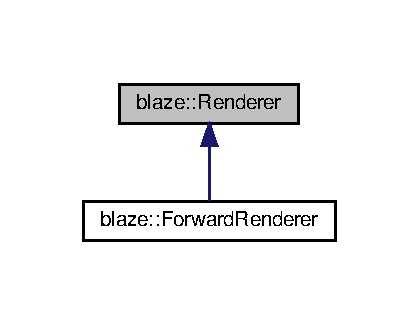
\includegraphics[width=201pt]{classblaze_1_1Renderer__inherit__graph}
\end{center}
\end{figure}
\subsection*{Public Member Functions}
\begin{DoxyCompactItemize}
\item 
\mbox{\Hypertarget{classblaze_1_1Renderer_ac23c0cb1d4b874ec4e695f14e5f5ed28}\label{classblaze_1_1Renderer_ac23c0cb1d4b874ec4e695f14e5f5ed28}} 
virtual \hyperlink{classblaze_1_1util_1_1PackedHandler}{util\+::\+Packed\+Handler}$<$ \hyperlink{classblaze_1_1Drawable}{Drawable} $\ast$ $>$\+::Handle {\bfseries submit} (\hyperlink{classblaze_1_1Drawable}{Drawable} $\ast$drawable)=0
\item 
\mbox{\Hypertarget{classblaze_1_1Renderer_aa62e515e52b6443b6d44889c323f4faa}\label{classblaze_1_1Renderer_aa62e515e52b6443b6d44889c323f4faa}} 
virtual void {\bfseries render\+Frame} ()=0
\item 
\mbox{\Hypertarget{classblaze_1_1Renderer_a03742f3dc6dddcf255619ee1e98e3ac5}\label{classblaze_1_1Renderer_a03742f3dc6dddcf255619ee1e98e3ac5}} 
virtual void {\bfseries set\+\_\+environment\+Descriptor} (Vk\+Descriptor\+Set env\+DS)=0
\item 
\mbox{\Hypertarget{classblaze_1_1Renderer_a72f5d088f85100cdac94005a76b36022}\label{classblaze_1_1Renderer_a72f5d088f85100cdac94005a76b36022}} 
virtual void {\bfseries set\+\_\+skybox\+Command} (const Render\+Command \&cmd)=0
\item 
\mbox{\Hypertarget{classblaze_1_1Renderer_a448ca277669a14598fc092c4dd487bb6}\label{classblaze_1_1Renderer_a448ca277669a14598fc092c4dd487bb6}} 
virtual void {\bfseries set\+\_\+camera\+U\+BO} (const \hyperlink{structblaze_1_1CameraUBlock}{Camera\+U\+Block} \&ubo)=0
\item 
\mbox{\Hypertarget{classblaze_1_1Renderer_aedb9fa390bfb08cc1a40b1a9342b59f4}\label{classblaze_1_1Renderer_aedb9fa390bfb08cc1a40b1a9342b59f4}} 
virtual void {\bfseries set\+\_\+camera} (\hyperlink{classblaze_1_1Camera}{Camera} $\ast$cam)=0
\item 
\mbox{\Hypertarget{classblaze_1_1Renderer_ac1083f14774761e2ae7e13e09bacb639}\label{classblaze_1_1Renderer_ac1083f14774761e2ae7e13e09bacb639}} 
virtual void {\bfseries set\+\_\+light\+U\+BO} (const \hyperlink{structblaze_1_1LightsUBlock}{Lights\+U\+Block} \&ubo)=0
\item 
\mbox{\Hypertarget{classblaze_1_1Renderer_a639f5f579b6fbfe3adfdc066bc3f2cbc}\label{classblaze_1_1Renderer_a639f5f579b6fbfe3adfdc066bc3f2cbc}} 
virtual void {\bfseries set\+\_\+settings\+U\+BO} (const \hyperlink{structblaze_1_1SettingsUBlock}{Settings\+U\+Block} \&ubo)=0
\item 
\mbox{\Hypertarget{classblaze_1_1Renderer_a99c966d3ba27170c87c73b475734b727}\label{classblaze_1_1Renderer_a99c966d3ba27170c87c73b475734b727}} 
virtual const Vk\+Descriptor\+Set\+Layout \& {\bfseries get\+\_\+material\+Layout} () const =0
\item 
\mbox{\Hypertarget{classblaze_1_1Renderer_aff4200083b396c6ed290251628736169}\label{classblaze_1_1Renderer_aff4200083b396c6ed290251628736169}} 
virtual const Vk\+Descriptor\+Set\+Layout \& {\bfseries get\+\_\+environment\+Layout} () const =0
\item 
\mbox{\Hypertarget{classblaze_1_1Renderer_a71ff380bf7a0ccf44d2d28f902b6aa6a}\label{classblaze_1_1Renderer_a71ff380bf7a0ccf44d2d28f902b6aa6a}} 
virtual \hyperlink{classblaze_1_1LightSystem}{Light\+System} \& {\bfseries get\+\_\+light\+System} ()=0
\item 
\mbox{\Hypertarget{classblaze_1_1Renderer_a2eb5167130e30ecbf59dd1b82f7104ec}\label{classblaze_1_1Renderer_a2eb5167130e30ecbf59dd1b82f7104ec}} 
virtual Vk\+Device {\bfseries get\+\_\+device} () const =0
\item 
\mbox{\Hypertarget{classblaze_1_1Renderer_ab72fd83ae03f68e72afde48ce241ae5a}\label{classblaze_1_1Renderer_ab72fd83ae03f68e72afde48ce241ae5a}} 
virtual const \hyperlink{classblaze_1_1Context}{Context} \& {\bfseries get\+\_\+context} () const =0
\item 
\mbox{\Hypertarget{classblaze_1_1Renderer_af6d6571efbdf5f4a0bbc4e619f59ccb4}\label{classblaze_1_1Renderer_af6d6571efbdf5f4a0bbc4e619f59ccb4}} 
virtual bool {\bfseries complete} () const =0
\end{DoxyCompactItemize}
\subsection*{Protected Types}
\begin{DoxyCompactItemize}
\item 
\mbox{\Hypertarget{classblaze_1_1Renderer_a168cdb0440569f01ce7bf630cb210277}\label{classblaze_1_1Renderer_a168cdb0440569f01ce7bf630cb210277}} 
using {\bfseries H\+Sub} = \hyperlink{classblaze_1_1util_1_1PackedHandler}{util\+::\+Packed\+Handler}$<$ \hyperlink{classblaze_1_1Drawable}{Drawable} $\ast$ $>$\+::Handle
\end{DoxyCompactItemize}


The documentation for this class was generated from the following file\+:\begin{DoxyCompactItemize}
\item 
Blaze/rendering/Renderer.\+hpp\end{DoxyCompactItemize}

\hypertarget{structblaze_1_1RendererUBlock}{}\section{blaze\+:\+:Renderer\+U\+Block Struct Reference}
\label{structblaze_1_1RendererUBlock}\index{blaze\+::\+Renderer\+U\+Block@{blaze\+::\+Renderer\+U\+Block}}


The actual data sent to the G\+PU.  




{\ttfamily \#include $<$Datatypes.\+hpp$>$}

\subsection*{Public Attributes}
\begin{DoxyCompactItemize}
\item 
\mbox{\Hypertarget{structblaze_1_1RendererUBlock_ac65ac83021eeffecb713e06e55962c4f}\label{structblaze_1_1RendererUBlock_ac65ac83021eeffecb713e06e55962c4f}} 
glm\+::mat4 {\bfseries view}
\item 
\mbox{\Hypertarget{structblaze_1_1RendererUBlock_aa7b90e03ccef455ca6a170a86bd80a27}\label{structblaze_1_1RendererUBlock_aa7b90e03ccef455ca6a170a86bd80a27}} 
glm\+::mat4 {\bfseries projection}
\item 
\mbox{\Hypertarget{structblaze_1_1RendererUBlock_a2e241d07462482fd2f5b0234b45713f6}\label{structblaze_1_1RendererUBlock_a2e241d07462482fd2f5b0234b45713f6}} 
glm\+::vec3 {\bfseries view\+Pos}
\item 
\mbox{\Hypertarget{structblaze_1_1RendererUBlock_a36afd164735550caa113bdca3dda1e62}\label{structblaze_1_1RendererUBlock_a36afd164735550caa113bdca3dda1e62}} 
float {\bfseries far\+Plane}
\item 
\mbox{\Hypertarget{structblaze_1_1RendererUBlock_a80d7fc6724c063497fc0b6fa1d69db5b}\label{structblaze_1_1RendererUBlock_a80d7fc6724c063497fc0b6fa1d69db5b}} 
glm\+::mat4 {\bfseries dir\+Light\+Transform} \mbox{[}M\+A\+X\+\_\+\+D\+I\+R\+\_\+\+L\+I\+G\+H\+TS\mbox{]}\mbox{[}M\+A\+X\+\_\+\+C\+S\+M\+\_\+\+S\+P\+L\+I\+TS\mbox{]}
\item 
\mbox{\Hypertarget{structblaze_1_1RendererUBlock_ada0b30a8e4dcc3adcfcdba842f2d0592}\label{structblaze_1_1RendererUBlock_ada0b30a8e4dcc3adcfcdba842f2d0592}} 
glm\+::vec4 {\bfseries light\+Dir} \mbox{[}M\+A\+X\+\_\+\+D\+I\+R\+\_\+\+L\+I\+G\+H\+TS\mbox{]}
\item 
\mbox{\Hypertarget{structblaze_1_1RendererUBlock_a8a7e1970d8aa9c9176cf100bf8620ba0}\label{structblaze_1_1RendererUBlock_a8a7e1970d8aa9c9176cf100bf8620ba0}} 
glm\+::vec4 {\bfseries csm\+Splits} \mbox{[}M\+A\+X\+\_\+\+C\+S\+M\+\_\+\+S\+P\+L\+I\+TS\mbox{]}
\item 
\mbox{\Hypertarget{structblaze_1_1RendererUBlock_a63b4ebd129dc7dc4d0e64a5618de79e1}\label{structblaze_1_1RendererUBlock_a63b4ebd129dc7dc4d0e64a5618de79e1}} 
glm\+::vec4 {\bfseries light\+Pos} \mbox{[}M\+A\+X\+\_\+\+P\+O\+I\+N\+T\+\_\+\+L\+I\+G\+H\+TS\mbox{]}
\item 
\mbox{\Hypertarget{structblaze_1_1RendererUBlock_aff5efd6364d49d0f2b58bc67128e3f04}\label{structblaze_1_1RendererUBlock_aff5efd6364d49d0f2b58bc67128e3f04}} 
int {\bfseries shadow\+Idx} \mbox{[}M\+A\+X\+\_\+\+P\+O\+I\+N\+T\+\_\+\+L\+I\+G\+H\+TS\mbox{]}
\item 
\mbox{\Hypertarget{structblaze_1_1RendererUBlock_ab2879d6607b7cddb5119e3b294d6d5bb}\label{structblaze_1_1RendererUBlock_ab2879d6607b7cddb5119e3b294d6d5bb}} 
int {\bfseries num\+Lights}
\item 
\mbox{\Hypertarget{structblaze_1_1RendererUBlock_a8daf3bed1ca11581c8c27bff0169e822}\label{structblaze_1_1RendererUBlock_a8daf3bed1ca11581c8c27bff0169e822}} 
int {\bfseries num\+Dir\+Lights}
\end{DoxyCompactItemize}


\subsection{Detailed Description}
The actual data sent to the G\+PU. 

This struct is a aggregation of \hyperlink{structblaze_1_1CameraUBlock}{Camera\+U\+Block} and \hyperlink{structblaze_1_1LightsUBlock}{Lights\+U\+Block}. They can be directly copied before sending to G\+PU view \hyperlink{classblaze_1_1UBO}{U\+BO} update.

\begin{DoxySeeAlso}{See also}
\hyperlink{structblaze_1_1CameraUBlock}{Camera\+U\+Block} 

\hyperlink{structblaze_1_1LightsUBlock}{Lights\+U\+Block} 
\end{DoxySeeAlso}


The documentation for this struct was generated from the following file\+:\begin{DoxyCompactItemize}
\item 
Blaze/Datatypes.\+hpp\end{DoxyCompactItemize}

\hypertarget{structblaze_1_1spirv_1_1RenderPass}{}\section{blaze\+:\+:spirv\+:\+:Render\+Pass Struct Reference}
\label{structblaze_1_1spirv_1_1RenderPass}\index{blaze\+::spirv\+::\+Render\+Pass@{blaze\+::spirv\+::\+Render\+Pass}}
\subsection*{Public Member Functions}
\begin{DoxyCompactItemize}
\item 
\mbox{\Hypertarget{structblaze_1_1spirv_1_1RenderPass_a8da5fb9d263414f56ea195869d90ba1e}\label{structblaze_1_1spirv_1_1RenderPass_a8da5fb9d263414f56ea195869d90ba1e}} 
Vk\+Render\+Pass {\bfseries get} () const
\end{DoxyCompactItemize}
\subsection*{Public Attributes}
\begin{DoxyCompactItemize}
\item 
\mbox{\Hypertarget{structblaze_1_1spirv_1_1RenderPass_acd04018e471fa9d900219fb67cc563ca}\label{structblaze_1_1spirv_1_1RenderPass_acd04018e471fa9d900219fb67cc563ca}} 
Framebuffer\+::\+Format\+ID {\bfseries fb\+Format}
\item 
\mbox{\Hypertarget{structblaze_1_1spirv_1_1RenderPass_abadce9b5d140e20e3fbf17bea4e62ff9}\label{structblaze_1_1spirv_1_1RenderPass_abadce9b5d140e20e3fbf17bea4e62ff9}} 
vkw\+::\+Render\+Pass {\bfseries render\+Pass}
\end{DoxyCompactItemize}


The documentation for this struct was generated from the following file\+:\begin{DoxyCompactItemize}
\item 
Blaze/spirv/Pipeline\+Factory.\+hpp\end{DoxyCompactItemize}

\hypertarget{structblaze_1_1spirv_1_1Shader_1_1Set}{}\section{blaze\+:\+:spirv\+:\+:Shader\+:\+:Set Struct Reference}
\label{structblaze_1_1spirv_1_1Shader_1_1Set}\index{blaze\+::spirv\+::\+Shader\+::\+Set@{blaze\+::spirv\+::\+Shader\+::\+Set}}
\subsection*{Classes}
\begin{DoxyCompactItemize}
\item 
struct \hyperlink{structblaze_1_1spirv_1_1Shader_1_1Set_1_1Format}{Format}
\end{DoxyCompactItemize}
\subsection*{Public Types}
\begin{DoxyCompactItemize}
\item 
\mbox{\Hypertarget{structblaze_1_1spirv_1_1Shader_1_1Set_a2033e85411f74aa7415d4c6cc33cdec3}\label{structblaze_1_1spirv_1_1Shader_1_1Set_a2033e85411f74aa7415d4c6cc33cdec3}} 
using {\bfseries Format\+ID} = uint32\+\_\+t
\end{DoxyCompactItemize}
\subsection*{Public Attributes}
\begin{DoxyCompactItemize}
\item 
\mbox{\Hypertarget{structblaze_1_1spirv_1_1Shader_1_1Set_a094121b02cb71d38ace665fd0f55dbb5}\label{structblaze_1_1spirv_1_1Shader_1_1Set_a094121b02cb71d38ace665fd0f55dbb5}} 
uint32\+\_\+t {\bfseries set} \{0\}
\item 
\mbox{\Hypertarget{structblaze_1_1spirv_1_1Shader_1_1Set_a15f1ceed83a85eb92cdb57e41c4f5a3d}\label{structblaze_1_1spirv_1_1Shader_1_1Set_a15f1ceed83a85eb92cdb57e41c4f5a3d}} 
std\+::vector$<$ \hyperlink{structblaze_1_1spirv_1_1UniformInfo}{Uniform\+Info} $>$ {\bfseries uniforms}
\item 
\mbox{\Hypertarget{structblaze_1_1spirv_1_1Shader_1_1Set_a3c5cdc3bc52c2f3e036fcb2dccbe8f4b}\label{structblaze_1_1spirv_1_1Shader_1_1Set_a3c5cdc3bc52c2f3e036fcb2dccbe8f4b}} 
vkw\+::\+Descriptor\+Set\+Layout {\bfseries layout}
\end{DoxyCompactItemize}


The documentation for this struct was generated from the following file\+:\begin{DoxyCompactItemize}
\item 
Blaze/spirv/Pipeline.\+hpp\end{DoxyCompactItemize}

\hypertarget{structblaze_1_1spirv_1_1SetSingleton}{}\section{blaze\+:\+:spirv\+:\+:Set\+Singleton Struct Reference}
\label{structblaze_1_1spirv_1_1SetSingleton}\index{blaze\+::spirv\+::\+Set\+Singleton@{blaze\+::spirv\+::\+Set\+Singleton}}
\subsection*{Public Member Functions}
\begin{DoxyCompactItemize}
\item 
\mbox{\Hypertarget{structblaze_1_1spirv_1_1SetSingleton_a1ce2da44b2eef618d2e4a342cf4c4f52}\label{structblaze_1_1spirv_1_1SetSingleton_a1ce2da44b2eef618d2e4a342cf4c4f52}} 
const Vk\+Descriptor\+Set \& {\bfseries get} () const
\item 
\mbox{\Hypertarget{structblaze_1_1spirv_1_1SetSingleton_a7767b199db5f71b8d81d7ffda56c2986}\label{structblaze_1_1spirv_1_1SetSingleton_a7767b199db5f71b8d81d7ffda56c2986}} 
const Vk\+Descriptor\+Set \& {\bfseries operator\mbox{[}$\,$\mbox{]}} (uint32\+\_\+t idx) const
\item 
\mbox{\Hypertarget{structblaze_1_1spirv_1_1SetSingleton_a56f29d08d24035df16ef6ad91bdffa1e}\label{structblaze_1_1spirv_1_1SetSingleton_a56f29d08d24035df16ef6ad91bdffa1e}} 
uint32\+\_\+t {\bfseries size} () const
\end{DoxyCompactItemize}
\subsection*{Public Attributes}
\begin{DoxyCompactItemize}
\item 
\mbox{\Hypertarget{structblaze_1_1spirv_1_1SetSingleton_a871ca54ecaaf9bf7111880af9673b8a8}\label{structblaze_1_1spirv_1_1SetSingleton_a871ca54ecaaf9bf7111880af9673b8a8}} 
Shader\+::\+Set\+::\+Format\+ID {\bfseries format\+ID}
\item 
\mbox{\Hypertarget{structblaze_1_1spirv_1_1SetSingleton_ae93988e6c27120dcbe6da5daae6e4ee8}\label{structblaze_1_1spirv_1_1SetSingleton_ae93988e6c27120dcbe6da5daae6e4ee8}} 
vkw\+::\+Descriptor\+Pool {\bfseries pool}
\item 
\mbox{\Hypertarget{structblaze_1_1spirv_1_1SetSingleton_a97d2c3727ca183de0127c34b761b57a4}\label{structblaze_1_1spirv_1_1SetSingleton_a97d2c3727ca183de0127c34b761b57a4}} 
vkw\+::\+Descriptor\+Set {\bfseries set}
\item 
\mbox{\Hypertarget{structblaze_1_1spirv_1_1SetSingleton_a5bc6c54fd40b83c451ca06235189524e}\label{structblaze_1_1spirv_1_1SetSingleton_a5bc6c54fd40b83c451ca06235189524e}} 
uint32\+\_\+t {\bfseries set\+Idx}
\end{DoxyCompactItemize}


The documentation for this struct was generated from the following file\+:\begin{DoxyCompactItemize}
\item 
Blaze/spirv/Pipeline\+Factory.\+hpp\end{DoxyCompactItemize}

\hypertarget{structblaze_1_1SettingsUBlock}{}\section{blaze\+:\+:Settings\+U\+Block Struct Reference}
\label{structblaze_1_1SettingsUBlock}\index{blaze\+::\+Settings\+U\+Block@{blaze\+::\+Settings\+U\+Block}}


Main display settings exposed to both Player and G\+PU Shader.  




{\ttfamily \#include $<$Datatypes.\+hpp$>$}

\subsection*{Public Types}
\begin{DoxyCompactItemize}
\item 
enum \hyperlink{structblaze_1_1SettingsUBlock_aa79fb061eee4130840f5ba7a8b36fdff}{View\+Texture\+Map} \+: int \{ \newline
{\bfseries V\+T\+M\+\_\+\+F\+U\+LL}, 
\hyperlink{structblaze_1_1SettingsUBlock_aa79fb061eee4130840f5ba7a8b36fdffa4090b24cd88f439ddf511b3ffc688698}{V\+T\+M\+\_\+\+D\+I\+F\+F\+U\+SE}, 
\hyperlink{structblaze_1_1SettingsUBlock_aa79fb061eee4130840f5ba7a8b36fdffa479628b3633fef2edb7665c884109c3f}{V\+T\+M\+\_\+\+N\+O\+R\+M\+AL}, 
\hyperlink{structblaze_1_1SettingsUBlock_aa79fb061eee4130840f5ba7a8b36fdffa7336c0dafc26bf28da993c839fac0253}{V\+T\+M\+\_\+\+M\+E\+T\+A\+L\+L\+IC}, 
\newline
\hyperlink{structblaze_1_1SettingsUBlock_aa79fb061eee4130840f5ba7a8b36fdffa373c6efa35d86a4552c64232508eb401}{V\+T\+M\+\_\+\+R\+O\+U\+G\+H\+N\+E\+SS}, 
\hyperlink{structblaze_1_1SettingsUBlock_aa79fb061eee4130840f5ba7a8b36fdffa6da51d120987704e0050ae2c4b09a670}{V\+T\+M\+\_\+\+AO}, 
\hyperlink{structblaze_1_1SettingsUBlock_aa79fb061eee4130840f5ba7a8b36fdffa4bfc17f599882a435c2e1eeef3cadc31}{V\+T\+M\+\_\+\+E\+M\+I\+S\+S\+I\+ON}, 
\hyperlink{structblaze_1_1SettingsUBlock_aa79fb061eee4130840f5ba7a8b36fdffaec02f1162167da8431b10d566a8fbf15}{V\+T\+M\+\_\+\+P\+O\+S\+I\+T\+I\+ON}, 
\newline
\hyperlink{structblaze_1_1SettingsUBlock_aa79fb061eee4130840f5ba7a8b36fdffafbc5b5961b516f23c4f4271fb2995d63}{V\+T\+M\+\_\+\+C\+A\+S\+C\+A\+DE}, 
\hyperlink{structblaze_1_1SettingsUBlock_aa79fb061eee4130840f5ba7a8b36fdffa4f3bec70ad9852c14460c0d8e94c1bac}{V\+T\+M\+\_\+\+M\+I\+SC}, 
\hyperlink{structblaze_1_1SettingsUBlock_aa79fb061eee4130840f5ba7a8b36fdffaab456181ac55efa82604a7523ae63495}{V\+T\+M\+\_\+\+M\+A\+X\+\_\+\+C\+O\+U\+NT}
 \}\begin{DoxyCompactList}\small\item\em Difference image maps or data visualizable on the screen. \end{DoxyCompactList}
\end{DoxyCompactItemize}
\subsection*{Public Attributes}
\begin{DoxyCompactItemize}
\item 
\mbox{\Hypertarget{structblaze_1_1SettingsUBlock_a29aa41ea92c2e3afca88f9d2510277ae}\label{structblaze_1_1SettingsUBlock_a29aa41ea92c2e3afca88f9d2510277ae}} 
enum \hyperlink{structblaze_1_1SettingsUBlock_aa79fb061eee4130840f5ba7a8b36fdff}{blaze\+::\+Settings\+U\+Block\+::\+View\+Texture\+Map} {\bfseries texture\+Map}
\item 
\mbox{\Hypertarget{structblaze_1_1SettingsUBlock_ad760b30cf669a5c0a0c78bf7bd7e79f3}\label{structblaze_1_1SettingsUBlock_ad760b30cf669a5c0a0c78bf7bd7e79f3}} 
\begin{tabbing}
xx\=xx\=xx\=xx\=xx\=xx\=xx\=xx\=xx\=\kill
union \{\\
\>bool {\bfseries B}\\
\>int {\bfseries I}\\
\} \hyperlink{structblaze_1_1SettingsUBlock_ad760b30cf669a5c0a0c78bf7bd7e79f3}{enableSkybox}\\

\end{tabbing}\begin{DoxyCompactList}\small\item\em Enable skybox. \end{DoxyCompactList}\item 
\mbox{\Hypertarget{structblaze_1_1SettingsUBlock_a44eab5d7c0a7dfededada2937e045705}\label{structblaze_1_1SettingsUBlock_a44eab5d7c0a7dfededada2937e045705}} 
\begin{tabbing}
xx\=xx\=xx\=xx\=xx\=xx\=xx\=xx\=xx\=\kill
union \{\\
\>bool {\bfseries B}\\
\>int {\bfseries I}\\
\} \hyperlink{structblaze_1_1SettingsUBlock_a44eab5d7c0a7dfededada2937e045705}{enableIBL}\\

\end{tabbing}\begin{DoxyCompactList}\small\item\em Enable I\+BL. \end{DoxyCompactList}\item 
\mbox{\Hypertarget{structblaze_1_1SettingsUBlock_a29dfda46fbf1c291506a57d5abc07423}\label{structblaze_1_1SettingsUBlock_a29dfda46fbf1c291506a57d5abc07423}} 
float \hyperlink{structblaze_1_1SettingsUBlock_a29dfda46fbf1c291506a57d5abc07423}{exposure} \{4.\+5f\}
\begin{DoxyCompactList}\small\item\em Exposure. \end{DoxyCompactList}\item 
\mbox{\Hypertarget{structblaze_1_1SettingsUBlock_ae9af586007d118e4253937aff6a4c92a}\label{structblaze_1_1SettingsUBlock_ae9af586007d118e4253937aff6a4c92a}} 
float \hyperlink{structblaze_1_1SettingsUBlock_ae9af586007d118e4253937aff6a4c92a}{gamma} \{2.\+2f\}
\begin{DoxyCompactList}\small\item\em Gamma. \end{DoxyCompactList}\end{DoxyCompactItemize}


\subsection{Detailed Description}
Main display settings exposed to both Player and G\+PU Shader. 

The component of the \hyperlink{classblaze_1_1GUI}{G\+UI} settings that are updated to the G\+PU. Used for shading options or debug displays. 

\subsection{Member Enumeration Documentation}
\mbox{\Hypertarget{structblaze_1_1SettingsUBlock_aa79fb061eee4130840f5ba7a8b36fdff}\label{structblaze_1_1SettingsUBlock_aa79fb061eee4130840f5ba7a8b36fdff}} 
\index{blaze\+::\+Settings\+U\+Block@{blaze\+::\+Settings\+U\+Block}!View\+Texture\+Map@{View\+Texture\+Map}}
\index{View\+Texture\+Map@{View\+Texture\+Map}!blaze\+::\+Settings\+U\+Block@{blaze\+::\+Settings\+U\+Block}}
\subsubsection{\texorpdfstring{View\+Texture\+Map}{ViewTextureMap}}
{\footnotesize\ttfamily enum \hyperlink{structblaze_1_1SettingsUBlock_aa79fb061eee4130840f5ba7a8b36fdff}{blaze\+::\+Settings\+U\+Block\+::\+View\+Texture\+Map} \+: int}



Difference image maps or data visualizable on the screen. 

\begin{DoxyEnumFields}{Enumerator}
\raisebox{\heightof{T}}[0pt][0pt]{\index{V\+T\+M\+\_\+\+D\+I\+F\+F\+U\+SE@{V\+T\+M\+\_\+\+D\+I\+F\+F\+U\+SE}!blaze\+::\+Settings\+U\+Block@{blaze\+::\+Settings\+U\+Block}}\index{blaze\+::\+Settings\+U\+Block@{blaze\+::\+Settings\+U\+Block}!V\+T\+M\+\_\+\+D\+I\+F\+F\+U\+SE@{V\+T\+M\+\_\+\+D\+I\+F\+F\+U\+SE}}}\mbox{\Hypertarget{structblaze_1_1SettingsUBlock_aa79fb061eee4130840f5ba7a8b36fdffa4090b24cd88f439ddf511b3ffc688698}\label{structblaze_1_1SettingsUBlock_aa79fb061eee4130840f5ba7a8b36fdffa4090b24cd88f439ddf511b3ffc688698}} 
V\+T\+M\+\_\+\+D\+I\+F\+F\+U\+SE&$<$ Full Render. \\
\hline

\raisebox{\heightof{T}}[0pt][0pt]{\index{V\+T\+M\+\_\+\+N\+O\+R\+M\+AL@{V\+T\+M\+\_\+\+N\+O\+R\+M\+AL}!blaze\+::\+Settings\+U\+Block@{blaze\+::\+Settings\+U\+Block}}\index{blaze\+::\+Settings\+U\+Block@{blaze\+::\+Settings\+U\+Block}!V\+T\+M\+\_\+\+N\+O\+R\+M\+AL@{V\+T\+M\+\_\+\+N\+O\+R\+M\+AL}}}\mbox{\Hypertarget{structblaze_1_1SettingsUBlock_aa79fb061eee4130840f5ba7a8b36fdffa479628b3633fef2edb7665c884109c3f}\label{structblaze_1_1SettingsUBlock_aa79fb061eee4130840f5ba7a8b36fdffa479628b3633fef2edb7665c884109c3f}} 
V\+T\+M\+\_\+\+N\+O\+R\+M\+AL&$<$ Show only albedo/diffuse maps. \\
\hline

\raisebox{\heightof{T}}[0pt][0pt]{\index{V\+T\+M\+\_\+\+M\+E\+T\+A\+L\+L\+IC@{V\+T\+M\+\_\+\+M\+E\+T\+A\+L\+L\+IC}!blaze\+::\+Settings\+U\+Block@{blaze\+::\+Settings\+U\+Block}}\index{blaze\+::\+Settings\+U\+Block@{blaze\+::\+Settings\+U\+Block}!V\+T\+M\+\_\+\+M\+E\+T\+A\+L\+L\+IC@{V\+T\+M\+\_\+\+M\+E\+T\+A\+L\+L\+IC}}}\mbox{\Hypertarget{structblaze_1_1SettingsUBlock_aa79fb061eee4130840f5ba7a8b36fdffa7336c0dafc26bf28da993c839fac0253}\label{structblaze_1_1SettingsUBlock_aa79fb061eee4130840f5ba7a8b36fdffa7336c0dafc26bf28da993c839fac0253}} 
V\+T\+M\+\_\+\+M\+E\+T\+A\+L\+L\+IC&$<$ Show only the world space normals. \\
\hline

\raisebox{\heightof{T}}[0pt][0pt]{\index{V\+T\+M\+\_\+\+R\+O\+U\+G\+H\+N\+E\+SS@{V\+T\+M\+\_\+\+R\+O\+U\+G\+H\+N\+E\+SS}!blaze\+::\+Settings\+U\+Block@{blaze\+::\+Settings\+U\+Block}}\index{blaze\+::\+Settings\+U\+Block@{blaze\+::\+Settings\+U\+Block}!V\+T\+M\+\_\+\+R\+O\+U\+G\+H\+N\+E\+SS@{V\+T\+M\+\_\+\+R\+O\+U\+G\+H\+N\+E\+SS}}}\mbox{\Hypertarget{structblaze_1_1SettingsUBlock_aa79fb061eee4130840f5ba7a8b36fdffa373c6efa35d86a4552c64232508eb401}\label{structblaze_1_1SettingsUBlock_aa79fb061eee4130840f5ba7a8b36fdffa373c6efa35d86a4552c64232508eb401}} 
V\+T\+M\+\_\+\+R\+O\+U\+G\+H\+N\+E\+SS&$<$ Show only the metallicity. \\
\hline

\raisebox{\heightof{T}}[0pt][0pt]{\index{V\+T\+M\+\_\+\+AO@{V\+T\+M\+\_\+\+AO}!blaze\+::\+Settings\+U\+Block@{blaze\+::\+Settings\+U\+Block}}\index{blaze\+::\+Settings\+U\+Block@{blaze\+::\+Settings\+U\+Block}!V\+T\+M\+\_\+\+AO@{V\+T\+M\+\_\+\+AO}}}\mbox{\Hypertarget{structblaze_1_1SettingsUBlock_aa79fb061eee4130840f5ba7a8b36fdffa6da51d120987704e0050ae2c4b09a670}\label{structblaze_1_1SettingsUBlock_aa79fb061eee4130840f5ba7a8b36fdffa6da51d120987704e0050ae2c4b09a670}} 
V\+T\+M\+\_\+\+AO&$<$ Show only the roughness. \\
\hline

\raisebox{\heightof{T}}[0pt][0pt]{\index{V\+T\+M\+\_\+\+E\+M\+I\+S\+S\+I\+ON@{V\+T\+M\+\_\+\+E\+M\+I\+S\+S\+I\+ON}!blaze\+::\+Settings\+U\+Block@{blaze\+::\+Settings\+U\+Block}}\index{blaze\+::\+Settings\+U\+Block@{blaze\+::\+Settings\+U\+Block}!V\+T\+M\+\_\+\+E\+M\+I\+S\+S\+I\+ON@{V\+T\+M\+\_\+\+E\+M\+I\+S\+S\+I\+ON}}}\mbox{\Hypertarget{structblaze_1_1SettingsUBlock_aa79fb061eee4130840f5ba7a8b36fdffa4bfc17f599882a435c2e1eeef3cadc31}\label{structblaze_1_1SettingsUBlock_aa79fb061eee4130840f5ba7a8b36fdffa4bfc17f599882a435c2e1eeef3cadc31}} 
V\+T\+M\+\_\+\+E\+M\+I\+S\+S\+I\+ON&$<$ Show only the ambient occlusion maps. \\
\hline

\raisebox{\heightof{T}}[0pt][0pt]{\index{V\+T\+M\+\_\+\+P\+O\+S\+I\+T\+I\+ON@{V\+T\+M\+\_\+\+P\+O\+S\+I\+T\+I\+ON}!blaze\+::\+Settings\+U\+Block@{blaze\+::\+Settings\+U\+Block}}\index{blaze\+::\+Settings\+U\+Block@{blaze\+::\+Settings\+U\+Block}!V\+T\+M\+\_\+\+P\+O\+S\+I\+T\+I\+ON@{V\+T\+M\+\_\+\+P\+O\+S\+I\+T\+I\+ON}}}\mbox{\Hypertarget{structblaze_1_1SettingsUBlock_aa79fb061eee4130840f5ba7a8b36fdffaec02f1162167da8431b10d566a8fbf15}\label{structblaze_1_1SettingsUBlock_aa79fb061eee4130840f5ba7a8b36fdffaec02f1162167da8431b10d566a8fbf15}} 
V\+T\+M\+\_\+\+P\+O\+S\+I\+T\+I\+ON&$<$ Show only the emissions. \\
\hline

\raisebox{\heightof{T}}[0pt][0pt]{\index{V\+T\+M\+\_\+\+C\+A\+S\+C\+A\+DE@{V\+T\+M\+\_\+\+C\+A\+S\+C\+A\+DE}!blaze\+::\+Settings\+U\+Block@{blaze\+::\+Settings\+U\+Block}}\index{blaze\+::\+Settings\+U\+Block@{blaze\+::\+Settings\+U\+Block}!V\+T\+M\+\_\+\+C\+A\+S\+C\+A\+DE@{V\+T\+M\+\_\+\+C\+A\+S\+C\+A\+DE}}}\mbox{\Hypertarget{structblaze_1_1SettingsUBlock_aa79fb061eee4130840f5ba7a8b36fdffafbc5b5961b516f23c4f4271fb2995d63}\label{structblaze_1_1SettingsUBlock_aa79fb061eee4130840f5ba7a8b36fdffafbc5b5961b516f23c4f4271fb2995d63}} 
V\+T\+M\+\_\+\+C\+A\+S\+C\+A\+DE&$<$ Show position coordinates normalized by far plane. \\
\hline

\raisebox{\heightof{T}}[0pt][0pt]{\index{V\+T\+M\+\_\+\+M\+I\+SC@{V\+T\+M\+\_\+\+M\+I\+SC}!blaze\+::\+Settings\+U\+Block@{blaze\+::\+Settings\+U\+Block}}\index{blaze\+::\+Settings\+U\+Block@{blaze\+::\+Settings\+U\+Block}!V\+T\+M\+\_\+\+M\+I\+SC@{V\+T\+M\+\_\+\+M\+I\+SC}}}\mbox{\Hypertarget{structblaze_1_1SettingsUBlock_aa79fb061eee4130840f5ba7a8b36fdffa4f3bec70ad9852c14460c0d8e94c1bac}\label{structblaze_1_1SettingsUBlock_aa79fb061eee4130840f5ba7a8b36fdffa4f3bec70ad9852c14460c0d8e94c1bac}} 
V\+T\+M\+\_\+\+M\+I\+SC&$<$ Show the C\+SM splits overlay on the render. \\
\hline

\raisebox{\heightof{T}}[0pt][0pt]{\index{V\+T\+M\+\_\+\+M\+A\+X\+\_\+\+C\+O\+U\+NT@{V\+T\+M\+\_\+\+M\+A\+X\+\_\+\+C\+O\+U\+NT}!blaze\+::\+Settings\+U\+Block@{blaze\+::\+Settings\+U\+Block}}\index{blaze\+::\+Settings\+U\+Block@{blaze\+::\+Settings\+U\+Block}!V\+T\+M\+\_\+\+M\+A\+X\+\_\+\+C\+O\+U\+NT@{V\+T\+M\+\_\+\+M\+A\+X\+\_\+\+C\+O\+U\+NT}}}\mbox{\Hypertarget{structblaze_1_1SettingsUBlock_aa79fb061eee4130840f5ba7a8b36fdffaab456181ac55efa82604a7523ae63495}\label{structblaze_1_1SettingsUBlock_aa79fb061eee4130840f5ba7a8b36fdffaab456181ac55efa82604a7523ae63495}} 
V\+T\+M\+\_\+\+M\+A\+X\+\_\+\+C\+O\+U\+NT&$<$ Misc \\
\hline

\end{DoxyEnumFields}


The documentation for this struct was generated from the following file\+:\begin{DoxyCompactItemize}
\item 
Blaze/Datatypes.\+hpp\end{DoxyCompactItemize}

\hypertarget{structblaze_1_1spirv_1_1SetVector}{}\section{blaze\+:\+:spirv\+:\+:Set\+Vector Struct Reference}
\label{structblaze_1_1spirv_1_1SetVector}\index{blaze\+::spirv\+::\+Set\+Vector@{blaze\+::spirv\+::\+Set\+Vector}}
\subsection*{Public Member Functions}
\begin{DoxyCompactItemize}
\item 
\mbox{\Hypertarget{structblaze_1_1spirv_1_1SetVector_a4b9598732811653172d5c6904da02406}\label{structblaze_1_1spirv_1_1SetVector_a4b9598732811653172d5c6904da02406}} 
const Vk\+Descriptor\+Set \& {\bfseries operator\mbox{[}$\,$\mbox{]}} (uint32\+\_\+t idx) const
\item 
\mbox{\Hypertarget{structblaze_1_1spirv_1_1SetVector_ab0d7db43f84e0a39019b55eef4890f99}\label{structblaze_1_1spirv_1_1SetVector_ab0d7db43f84e0a39019b55eef4890f99}} 
uint32\+\_\+t {\bfseries size} () const
\end{DoxyCompactItemize}
\subsection*{Public Attributes}
\begin{DoxyCompactItemize}
\item 
\mbox{\Hypertarget{structblaze_1_1spirv_1_1SetVector_a317f8d377122785c99cc0e9cef2e2195}\label{structblaze_1_1spirv_1_1SetVector_a317f8d377122785c99cc0e9cef2e2195}} 
Shader\+::\+Set\+::\+Format\+ID {\bfseries format\+ID}
\item 
\mbox{\Hypertarget{structblaze_1_1spirv_1_1SetVector_a5bd781f225cca55af5990d2045225a42}\label{structblaze_1_1spirv_1_1SetVector_a5bd781f225cca55af5990d2045225a42}} 
vkw\+::\+Descriptor\+Pool {\bfseries pool}
\item 
\mbox{\Hypertarget{structblaze_1_1spirv_1_1SetVector_a1826547495d44b376c29ec8c7b0d4ff0}\label{structblaze_1_1spirv_1_1SetVector_a1826547495d44b376c29ec8c7b0d4ff0}} 
vkw\+::\+Descriptor\+Set\+Vector {\bfseries sets}
\item 
\mbox{\Hypertarget{structblaze_1_1spirv_1_1SetVector_a0632f6d397163952e42136528b6639ab}\label{structblaze_1_1spirv_1_1SetVector_a0632f6d397163952e42136528b6639ab}} 
uint32\+\_\+t {\bfseries set\+Idx}
\end{DoxyCompactItemize}


The documentation for this struct was generated from the following file\+:\begin{DoxyCompactItemize}
\item 
Blaze/spirv/Pipeline\+Factory.\+hpp\end{DoxyCompactItemize}

\hypertarget{structblaze_1_1spirv_1_1Shader}{}\section{blaze\+:\+:spirv\+:\+:Shader Struct Reference}
\label{structblaze_1_1spirv_1_1Shader}\index{blaze\+::spirv\+::\+Shader@{blaze\+::spirv\+::\+Shader}}


Collaboration diagram for blaze\+:\+:spirv\+:\+:Shader\+:\nopagebreak
\begin{figure}[H]
\begin{center}
\leavevmode
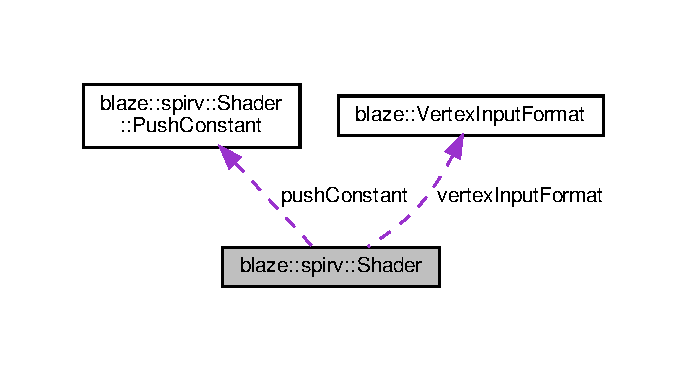
\includegraphics[width=330pt]{structblaze_1_1spirv_1_1Shader__coll__graph}
\end{center}
\end{figure}
\subsection*{Classes}
\begin{DoxyCompactItemize}
\item 
struct \hyperlink{structblaze_1_1spirv_1_1Shader_1_1PushConstant}{Push\+Constant}
\item 
struct \hyperlink{structblaze_1_1spirv_1_1Shader_1_1Set}{Set}
\end{DoxyCompactItemize}
\subsection*{Public Member Functions}
\begin{DoxyCompactItemize}
\item 
\mbox{\Hypertarget{structblaze_1_1spirv_1_1Shader_a2d981cbb6738aefad91e9badb730cd1e}\label{structblaze_1_1spirv_1_1Shader_a2d981cbb6738aefad91e9badb730cd1e}} 
bool {\bfseries valid} () const
\end{DoxyCompactItemize}
\subsection*{Public Attributes}
\begin{DoxyCompactItemize}
\item 
\mbox{\Hypertarget{structblaze_1_1spirv_1_1Shader_ab64ee55b8c711d11fed9e527d1c785eb}\label{structblaze_1_1spirv_1_1Shader_ab64ee55b8c711d11fed9e527d1c785eb}} 
\hyperlink{structblaze_1_1VertexInputFormat}{Vertex\+Input\+Format} {\bfseries vertex\+Input\+Format}
\item 
\mbox{\Hypertarget{structblaze_1_1spirv_1_1Shader_a8722e394db106c5ed51ca05e056d880b}\label{structblaze_1_1spirv_1_1Shader_a8722e394db106c5ed51ca05e056d880b}} 
int {\bfseries fragment\+Outputs}
\item 
\mbox{\Hypertarget{structblaze_1_1spirv_1_1Shader_a82b2ed73c8589a54620e479162b8f41a}\label{structblaze_1_1spirv_1_1Shader_a82b2ed73c8589a54620e479162b8f41a}} 
\hyperlink{structblaze_1_1spirv_1_1Shader_1_1PushConstant}{Push\+Constant} {\bfseries push\+Constant}
\item 
\mbox{\Hypertarget{structblaze_1_1spirv_1_1Shader_a6588c3eabc1b7e90e6e2b6533b7180d6}\label{structblaze_1_1spirv_1_1Shader_a6588c3eabc1b7e90e6e2b6533b7180d6}} 
bool {\bfseries is\+Compute} = false
\item 
\mbox{\Hypertarget{structblaze_1_1spirv_1_1Shader_ae46b7d5db6c1f5243dc309337c113994}\label{structblaze_1_1spirv_1_1Shader_ae46b7d5db6c1f5243dc309337c113994}} 
std\+::vector$<$ \hyperlink{structblaze_1_1spirv_1_1Shader_1_1Set}{Set} $>$ {\bfseries sets}
\item 
\mbox{\Hypertarget{structblaze_1_1spirv_1_1Shader_a103de1b45c2f19d4fb7d6698d36c4a96}\label{structblaze_1_1spirv_1_1Shader_a103de1b45c2f19d4fb7d6698d36c4a96}} 
std\+::vector$<$ Set\+::\+Format\+ID $>$ {\bfseries set\+Formats}
\item 
\mbox{\Hypertarget{structblaze_1_1spirv_1_1Shader_a8f8466e238f04e9932ae956db352e39d}\label{structblaze_1_1spirv_1_1Shader_a8f8466e238f04e9932ae956db352e39d}} 
std\+::vector$<$ Vk\+Pipeline\+Shader\+Stage\+Create\+Info $>$ {\bfseries pipeline\+Stages}
\item 
\mbox{\Hypertarget{structblaze_1_1spirv_1_1Shader_af193b80af1de1276aeab7a30122f0c84}\label{structblaze_1_1spirv_1_1Shader_af193b80af1de1276aeab7a30122f0c84}} 
std\+::vector$<$ vkw\+::\+Shader\+Module $>$ {\bfseries shader\+Modules}
\item 
\mbox{\Hypertarget{structblaze_1_1spirv_1_1Shader_acc55ff4291f82c265e42db7ffbd2549c}\label{structblaze_1_1spirv_1_1Shader_acc55ff4291f82c265e42db7ffbd2549c}} 
vkw\+::\+Pipeline\+Layout {\bfseries pipeline\+Layout}
\item 
\mbox{\Hypertarget{structblaze_1_1spirv_1_1Shader_a6bc8e60d9b3ae63f80e92f563508df00}\label{structblaze_1_1spirv_1_1Shader_a6bc8e60d9b3ae63f80e92f563508df00}} 
std\+::map$<$ std\+::string, std\+::pair$<$ uint32\+\_\+t, uint32\+\_\+t $>$ $>$ {\bfseries uniform\+Locations}
\end{DoxyCompactItemize}
\subsection*{Friends}
\begin{DoxyCompactItemize}
\item 
\mbox{\Hypertarget{structblaze_1_1spirv_1_1Shader_a7cd5e76e0aadd59a743317d722b404db}\label{structblaze_1_1spirv_1_1Shader_a7cd5e76e0aadd59a743317d722b404db}} 
std\+::ostream \& {\bfseries operator$<$$<$} (std\+::ostream \&out, const \hyperlink{structblaze_1_1spirv_1_1Shader}{Shader} \&shader)
\end{DoxyCompactItemize}


The documentation for this struct was generated from the following file\+:\begin{DoxyCompactItemize}
\item 
Blaze/spirv/Pipeline.\+hpp\end{DoxyCompactItemize}

\hypertarget{structblaze_1_1spirv_1_1ShaderStageData}{}\section{blaze\+:\+:spirv\+:\+:Shader\+Stage\+Data Struct Reference}
\label{structblaze_1_1spirv_1_1ShaderStageData}\index{blaze\+::spirv\+::\+Shader\+Stage\+Data@{blaze\+::spirv\+::\+Shader\+Stage\+Data}}
\subsection*{Public Member Functions}
\begin{DoxyCompactItemize}
\item 
\mbox{\Hypertarget{structblaze_1_1spirv_1_1ShaderStageData_a662a5b292a2bad929c7d516701419bd3}\label{structblaze_1_1spirv_1_1ShaderStageData_a662a5b292a2bad929c7d516701419bd3}} 
uint32\+\_\+t {\bfseries size} () const
\item 
\mbox{\Hypertarget{structblaze_1_1spirv_1_1ShaderStageData_aff9ed5ed66f552994cae6afb3e8093e6}\label{structblaze_1_1spirv_1_1ShaderStageData_aff9ed5ed66f552994cae6afb3e8093e6}} 
const void $\ast$ {\bfseries code} () const
\end{DoxyCompactItemize}
\subsection*{Public Attributes}
\begin{DoxyCompactItemize}
\item 
\mbox{\Hypertarget{structblaze_1_1spirv_1_1ShaderStageData_a70dc204fcb4a786ac84f96b7419bac90}\label{structblaze_1_1spirv_1_1ShaderStageData_a70dc204fcb4a786ac84f96b7419bac90}} 
Vk\+Shader\+Stage\+Flag\+Bits {\bfseries stage}
\item 
\mbox{\Hypertarget{structblaze_1_1spirv_1_1ShaderStageData_aec317339cb259e4882e5cbd68bad2d35}\label{structblaze_1_1spirv_1_1ShaderStageData_aec317339cb259e4882e5cbd68bad2d35}} 
std\+::vector$<$ uint32\+\_\+t $>$ {\bfseries spirv}
\end{DoxyCompactItemize}


The documentation for this struct was generated from the following file\+:\begin{DoxyCompactItemize}
\item 
Blaze/spirv/Pipeline\+Factory.\+hpp\end{DoxyCompactItemize}

\hypertarget{structblaze_1_1ShadowPushConstantBlock}{}\section{blaze\+:\+:Shadow\+Push\+Constant\+Block Struct Reference}
\label{structblaze_1_1ShadowPushConstantBlock}\index{blaze\+::\+Shadow\+Push\+Constant\+Block@{blaze\+::\+Shadow\+Push\+Constant\+Block}}


P\+CB for sending projection matrix and position to the G\+PU.  




{\ttfamily \#include $<$Datatypes.\+hpp$>$}

\subsection*{Public Attributes}
\begin{DoxyCompactItemize}
\item 
\mbox{\Hypertarget{structblaze_1_1ShadowPushConstantBlock_af459f4655cc68b9394867648fcb48fb9}\label{structblaze_1_1ShadowPushConstantBlock_af459f4655cc68b9394867648fcb48fb9}} 
glm\+::mat4 {\bfseries projection}
\item 
\mbox{\Hypertarget{structblaze_1_1ShadowPushConstantBlock_a2215b39c0cbb7d737a98702e28f07032}\label{structblaze_1_1ShadowPushConstantBlock_a2215b39c0cbb7d737a98702e28f07032}} 
glm\+::vec3 {\bfseries position}
\end{DoxyCompactItemize}


\subsection{Detailed Description}
P\+CB for sending projection matrix and position to the G\+PU. 

During omnidirectional shadow mapping, \hyperlink{structblaze_1_1ShadowUBlock}{Shadow\+U\+Block} provides The view matrix for each face of the cubemap. The Projection and position change per shadow, and hence are a part of the P\+CB 

The documentation for this struct was generated from the following file\+:\begin{DoxyCompactItemize}
\item 
Blaze/Datatypes.\+hpp\end{DoxyCompactItemize}

\hypertarget{structblaze_1_1ShadowUBlock}{}\section{blaze\+:\+:Shadow\+U\+Block Struct Reference}
\label{structblaze_1_1ShadowUBlock}\index{blaze\+::\+Shadow\+U\+Block@{blaze\+::\+Shadow\+U\+Block}}


The data sent to the omnidirectional shadow shaders.  




{\ttfamily \#include $<$Datatypes.\+hpp$>$}

\subsection*{Public Attributes}
\begin{DoxyCompactItemize}
\item 
\mbox{\Hypertarget{structblaze_1_1ShadowUBlock_ad2b3099b1e0880eb3d2b09684fa9cf51}\label{structblaze_1_1ShadowUBlock_ad2b3099b1e0880eb3d2b09684fa9cf51}} 
glm\+::mat4 \hyperlink{structblaze_1_1ShadowUBlock_ad2b3099b1e0880eb3d2b09684fa9cf51}{view} \mbox{[}6\mbox{]}
\begin{DoxyCompactList}\small\item\em View matrices to look at each direction. \end{DoxyCompactList}\end{DoxyCompactItemize}


\subsection{Detailed Description}
The data sent to the omnidirectional shadow shaders. 

\begin{DoxyNote}{Note}
Needs Projection matrix from \hyperlink{structblaze_1_1ShadowPushConstantBlock}{Shadow\+Push\+Constant\+Block} 
\end{DoxyNote}


The documentation for this struct was generated from the following file\+:\begin{DoxyCompactItemize}
\item 
Blaze/Datatypes.\+hpp\end{DoxyCompactItemize}

\hypertarget{classblaze_1_1Swapchain}{}\section{blaze\+:\+:Swapchain Class Reference}
\label{classblaze_1_1Swapchain}\index{blaze\+::\+Swapchain@{blaze\+::\+Swapchain}}


Wrapper for all swapchain related objects.  




{\ttfamily \#include $<$Swapchain.\+hpp$>$}

\subsection*{Public Member Functions}
\begin{DoxyCompactItemize}
\item 
\mbox{\Hypertarget{classblaze_1_1Swapchain_ada1346a550e854f89adc30f47866e585}\label{classblaze_1_1Swapchain_ada1346a550e854f89adc30f47866e585}} 
\hyperlink{classblaze_1_1Swapchain_ada1346a550e854f89adc30f47866e585}{Swapchain} () noexcept
\begin{DoxyCompactList}\small\item\em Default Constructor. \end{DoxyCompactList}\item 
\hyperlink{classblaze_1_1Swapchain_a92cae631c3a1b925686a1836a3b15e09}{Swapchain} (const \hyperlink{classblaze_1_1Context}{Context} $\ast$context) noexcept
\begin{DoxyCompactList}\small\item\em Main constructor. \end{DoxyCompactList}\item 
void \hyperlink{classblaze_1_1Swapchain_a1ab37b70fcc07c5dea24486087011314}{recreate} (const \hyperlink{classblaze_1_1Context}{Context} $\ast$context) noexcept
\begin{DoxyCompactList}\small\item\em Recreates the swapchain due to changes in screen size etc. \end{DoxyCompactList}\end{DoxyCompactItemize}
\begin{Indent}\textbf{ Getters}\par
{\em Getters for private members. }\begin{DoxyCompactItemize}
\item 
\mbox{\Hypertarget{classblaze_1_1Swapchain_a9a2fe335a790ad8581165bc353d26569}\label{classblaze_1_1Swapchain_a9a2fe335a790ad8581165bc353d26569}} 
const Vk\+Swapchain\+K\+HR \& {\bfseries get\+\_\+swapchain} () const
\item 
\mbox{\Hypertarget{classblaze_1_1Swapchain_a103a3cebe7b75028eeb9c39c16038d86}\label{classblaze_1_1Swapchain_a103a3cebe7b75028eeb9c39c16038d86}} 
const Vk\+Format \& {\bfseries get\+\_\+format} () const
\item 
\mbox{\Hypertarget{classblaze_1_1Swapchain_a69bca799467458dc5a4fbeea81903d9e}\label{classblaze_1_1Swapchain_a69bca799467458dc5a4fbeea81903d9e}} 
const Vk\+Extent2D \& {\bfseries get\+\_\+extent} () const
\item 
\mbox{\Hypertarget{classblaze_1_1Swapchain_a7945c6e9ec1469f757cde951574ba56a}\label{classblaze_1_1Swapchain_a7945c6e9ec1469f757cde951574ba56a}} 
const std\+::vector$<$ Vk\+Image\+View $>$ \& {\bfseries get\+\_\+image\+Views} () const
\item 
\mbox{\Hypertarget{classblaze_1_1Swapchain_ad8ec74238cba2e2b5c99700e816677d0}\label{classblaze_1_1Swapchain_ad8ec74238cba2e2b5c99700e816677d0}} 
const Vk\+Image\+View \& {\bfseries get\+\_\+image\+View} (uint32\+\_\+t index) const
\item 
\mbox{\Hypertarget{classblaze_1_1Swapchain_a91a4f7baa440ae11d61fe81a59c1aa33}\label{classblaze_1_1Swapchain_a91a4f7baa440ae11d61fe81a59c1aa33}} 
const uint32\+\_\+t \& {\bfseries get\+\_\+image\+Count} () const
\end{DoxyCompactItemize}
\end{Indent}
\begin{Indent}\textbf{ Move Constructors}\par
{\em All the move constructors, copy is deleted. }\begin{DoxyCompactItemize}
\item 
\mbox{\Hypertarget{classblaze_1_1Swapchain_a7fb4cafc77a13f8f528f36cd1bfdef8e}\label{classblaze_1_1Swapchain_a7fb4cafc77a13f8f528f36cd1bfdef8e}} 
{\bfseries Swapchain} (\hyperlink{classblaze_1_1Swapchain}{Swapchain} \&\&other) noexcept
\item 
\mbox{\Hypertarget{classblaze_1_1Swapchain_a905a406ed42dba71fabfa376c91b093e}\label{classblaze_1_1Swapchain_a905a406ed42dba71fabfa376c91b093e}} 
\hyperlink{classblaze_1_1Swapchain}{Swapchain} \& {\bfseries operator=} (\hyperlink{classblaze_1_1Swapchain}{Swapchain} \&\&other) noexcept
\item 
\mbox{\Hypertarget{classblaze_1_1Swapchain_adc9e4978a3d87beade9512d2adc60ffc}\label{classblaze_1_1Swapchain_adc9e4978a3d87beade9512d2adc60ffc}} 
{\bfseries Swapchain} (const \hyperlink{classblaze_1_1Swapchain}{Swapchain} \&other)=delete
\item 
\mbox{\Hypertarget{classblaze_1_1Swapchain_a9502036a56c1dd2ca10e5fe273490986}\label{classblaze_1_1Swapchain_a9502036a56c1dd2ca10e5fe273490986}} 
\hyperlink{classblaze_1_1Swapchain}{Swapchain} \& {\bfseries operator=} (const \hyperlink{classblaze_1_1Swapchain}{Swapchain} \&other)=delete
\end{DoxyCompactItemize}
\end{Indent}


\subsection{Detailed Description}
Wrapper for all swapchain related objects. 

Contains the swapchain, the images, views, format and extent. 

\subsection{Constructor \& Destructor Documentation}
\mbox{\Hypertarget{classblaze_1_1Swapchain_a92cae631c3a1b925686a1836a3b15e09}\label{classblaze_1_1Swapchain_a92cae631c3a1b925686a1836a3b15e09}} 
\index{blaze\+::\+Swapchain@{blaze\+::\+Swapchain}!Swapchain@{Swapchain}}
\index{Swapchain@{Swapchain}!blaze\+::\+Swapchain@{blaze\+::\+Swapchain}}
\subsubsection{\texorpdfstring{Swapchain()}{Swapchain()}}
{\footnotesize\ttfamily blaze\+::\+Swapchain\+::\+Swapchain (\begin{DoxyParamCaption}\item[{const \hyperlink{classblaze_1_1Context}{Context} $\ast$}]{context }\end{DoxyParamCaption})\hspace{0.3cm}{\ttfamily [noexcept]}}



Main constructor. 


\begin{DoxyParams}{Parameters}
{\em context} & Pointer to the Vulkan \hyperlink{classblaze_1_1Context}{Context} in use. \\
\hline
\end{DoxyParams}


\subsection{Member Function Documentation}
\mbox{\Hypertarget{classblaze_1_1Swapchain_a1ab37b70fcc07c5dea24486087011314}\label{classblaze_1_1Swapchain_a1ab37b70fcc07c5dea24486087011314}} 
\index{blaze\+::\+Swapchain@{blaze\+::\+Swapchain}!recreate@{recreate}}
\index{recreate@{recreate}!blaze\+::\+Swapchain@{blaze\+::\+Swapchain}}
\subsubsection{\texorpdfstring{recreate()}{recreate()}}
{\footnotesize\ttfamily void blaze\+::\+Swapchain\+::recreate (\begin{DoxyParamCaption}\item[{const \hyperlink{classblaze_1_1Context}{Context} $\ast$}]{context }\end{DoxyParamCaption})\hspace{0.3cm}{\ttfamily [noexcept]}}



Recreates the swapchain due to changes in screen size etc. 


\begin{DoxyParams}{Parameters}
{\em context} & Pointer to the Vulkan \hyperlink{classblaze_1_1Context}{Context} in use. \\
\hline
\end{DoxyParams}


The documentation for this class was generated from the following files\+:\begin{DoxyCompactItemize}
\item 
Blaze/core/Swapchain.\+hpp\item 
Blaze/core/Swapchain.\+cpp\end{DoxyCompactItemize}

\hypertarget{structblaze_1_1util_1_1SwapchainSupportDetails}{}\section{blaze\+:\+:util\+:\+:Swapchain\+Support\+Details Struct Reference}
\label{structblaze_1_1util_1_1SwapchainSupportDetails}\index{blaze\+::util\+::\+Swapchain\+Support\+Details@{blaze\+::util\+::\+Swapchain\+Support\+Details}}


Holds supported swapchain features.  




{\ttfamily \#include $<$Device\+Selection.\+hpp$>$}

\subsection*{Public Attributes}
\begin{DoxyCompactItemize}
\item 
\mbox{\Hypertarget{structblaze_1_1util_1_1SwapchainSupportDetails_acb0776fd24647f6102e1e308efdfd25c}\label{structblaze_1_1util_1_1SwapchainSupportDetails_acb0776fd24647f6102e1e308efdfd25c}} 
Vk\+Surface\+Capabilities\+K\+HR {\bfseries capabilities} \{\}
\item 
\mbox{\Hypertarget{structblaze_1_1util_1_1SwapchainSupportDetails_a4bc20cacc83f2ae84dd4228211bc0529}\label{structblaze_1_1util_1_1SwapchainSupportDetails_a4bc20cacc83f2ae84dd4228211bc0529}} 
std\+::vector$<$ Vk\+Surface\+Format\+K\+HR $>$ {\bfseries formats}
\item 
\mbox{\Hypertarget{structblaze_1_1util_1_1SwapchainSupportDetails_a56b120c08340305a41a3fa534e2a598f}\label{structblaze_1_1util_1_1SwapchainSupportDetails_a56b120c08340305a41a3fa534e2a598f}} 
std\+::vector$<$ Vk\+Present\+Mode\+K\+HR $>$ {\bfseries present\+Modes}
\end{DoxyCompactItemize}


\subsection{Detailed Description}
Holds supported swapchain features. 

The documentation for this struct was generated from the following file\+:\begin{DoxyCompactItemize}
\item 
Blaze/util/Device\+Selection.\+hpp\end{DoxyCompactItemize}

\hypertarget{structblaze_1_1util_1_1Texture2CubemapInfo}{}\section{blaze\+:\+:util\+:\+:Texture2\+Cubemap\+Info$<$ P\+CB $>$ Class Template Reference}
\label{structblaze_1_1util_1_1Texture2CubemapInfo}\index{blaze\+::util\+::\+Texture2\+Cubemap\+Info$<$ P\+C\+B $>$@{blaze\+::util\+::\+Texture2\+Cubemap\+Info$<$ P\+C\+B $>$}}


The information to use for the processing.  




{\ttfamily \#include $<$processing.\+hpp$>$}

\subsection*{Public Attributes}
\begin{DoxyCompactItemize}
\item 
\mbox{\Hypertarget{structblaze_1_1util_1_1Texture2CubemapInfo_a58b6a2fc14400e6db29c239d40c9b0b2}\label{structblaze_1_1util_1_1Texture2CubemapInfo_a58b6a2fc14400e6db29c239d40c9b0b2}} 
std\+::string \hyperlink{structblaze_1_1util_1_1Texture2CubemapInfo_a58b6a2fc14400e6db29c239d40c9b0b2}{vert\+\_\+shader}
\begin{DoxyCompactList}\small\item\em The vertex shader to use. \end{DoxyCompactList}\item 
\mbox{\Hypertarget{structblaze_1_1util_1_1Texture2CubemapInfo_a50024fcdeeb6d7c4568c2ae6b77857b1}\label{structblaze_1_1util_1_1Texture2CubemapInfo_a50024fcdeeb6d7c4568c2ae6b77857b1}} 
std\+::string \hyperlink{structblaze_1_1util_1_1Texture2CubemapInfo_a50024fcdeeb6d7c4568c2ae6b77857b1}{frag\+\_\+shader}
\begin{DoxyCompactList}\small\item\em The fragment shader to use. \end{DoxyCompactList}\item 
\mbox{\Hypertarget{structblaze_1_1util_1_1Texture2CubemapInfo_a6a7353a2473bbb9bba4960b9160b69e0}\label{structblaze_1_1util_1_1Texture2CubemapInfo_a6a7353a2473bbb9bba4960b9160b69e0}} 
Vk\+Descriptor\+Set \hyperlink{structblaze_1_1util_1_1Texture2CubemapInfo_a6a7353a2473bbb9bba4960b9160b69e0}{descriptor}
\begin{DoxyCompactList}\small\item\em The descriptor to use. \end{DoxyCompactList}\item 
\mbox{\Hypertarget{structblaze_1_1util_1_1Texture2CubemapInfo_ae5917e354d24b4e6ad811f193cff85b4}\label{structblaze_1_1util_1_1Texture2CubemapInfo_ae5917e354d24b4e6ad811f193cff85b4}} 
Vk\+Descriptor\+Set\+Layout \hyperlink{structblaze_1_1util_1_1Texture2CubemapInfo_ae5917e354d24b4e6ad811f193cff85b4}{layout}
\begin{DoxyCompactList}\small\item\em The layout of the descriptor in use/. \end{DoxyCompactList}\item 
\mbox{\Hypertarget{structblaze_1_1util_1_1Texture2CubemapInfo_a618c03b5fcf899629143233a4fdf1053}\label{structblaze_1_1util_1_1Texture2CubemapInfo_a618c03b5fcf899629143233a4fdf1053}} 
uint32\+\_\+t \hyperlink{structblaze_1_1util_1_1Texture2CubemapInfo_a618c03b5fcf899629143233a4fdf1053}{cube\+\_\+side} \{512\}
\begin{DoxyCompactList}\small\item\em The size of the side of the cubemap. \end{DoxyCompactList}\item 
\mbox{\Hypertarget{structblaze_1_1util_1_1Texture2CubemapInfo_a6bf41f7f9f62e7e22c33aff36e6804fa}\label{structblaze_1_1util_1_1Texture2CubemapInfo_a6bf41f7f9f62e7e22c33aff36e6804fa}} 
P\+CB \hyperlink{structblaze_1_1util_1_1Texture2CubemapInfo_a6bf41f7f9f62e7e22c33aff36e6804fa}{pcb} \{\}
\begin{DoxyCompactList}\small\item\em The push constant block to push into the pipeline. \end{DoxyCompactList}\end{DoxyCompactItemize}


\subsection{Detailed Description}
\subsubsection*{template$<$typename P\+CB$>$\newline
class blaze\+::util\+::\+Texture2\+Cubemap\+Info$<$ P\+C\+B $>$}

The information to use for the processing. 


\begin{DoxyTemplParams}{Template Parameters}
{\em P\+CB} & The type of the struct used for P\+CB. \\
\hline
\end{DoxyTemplParams}


The documentation for this class was generated from the following file\+:\begin{DoxyCompactItemize}
\item 
Blaze/util/processing.\+hpp\end{DoxyCompactItemize}

\hypertarget{classblaze_1_1Texture2D}{}\section{blaze\+:\+:Texture2D Class Reference}
\label{classblaze_1_1Texture2D}\index{blaze\+::\+Texture2D@{blaze\+::\+Texture2D}}


A wrapper over a vulkan texture that contains all the required data.  




{\ttfamily \#include $<$Texture2\+D.\+hpp$>$}

\subsection*{Public Member Functions}
\begin{DoxyCompactItemize}
\item 
\mbox{\Hypertarget{classblaze_1_1Texture2D_ac2c630eccb2ac79ee331e03980622cc3}\label{classblaze_1_1Texture2D_ac2c630eccb2ac79ee331e03980622cc3}} 
\hyperlink{classblaze_1_1Texture2D_ac2c630eccb2ac79ee331e03980622cc3}{Texture2D} () noexcept
\begin{DoxyCompactList}\small\item\em Default Constructor. \end{DoxyCompactList}\item 
\hyperlink{classblaze_1_1Texture2D_ad3f7b6a52513786666cc64281a098d12}{Texture2D} (const \hyperlink{classblaze_1_1Context}{Context} $\ast$context, const \hyperlink{structblaze_1_1ImageData2D}{Image\+Data2D} \&image\+\_\+data, bool mipmapped=false)
\begin{DoxyCompactList}\small\item\em Constructor for the texture. \end{DoxyCompactList}\item 
bool \hyperlink{classblaze_1_1Texture2D_af8ce33dec5506e1f52df11f7aef8c9fc}{valid} () const
\begin{DoxyCompactList}\small\item\em Checks if a texture is valid and usable. \end{DoxyCompactList}\item 
void \hyperlink{classblaze_1_1Texture2D_a14cd835af0b1c5e137f10dbb7b968e83}{transfer\+Layout} (Vk\+Command\+Buffer cmdbuffer, Vk\+Image\+Layout new\+Image\+Layout, Vk\+Access\+Flags dst\+Access=0, Vk\+Pipeline\+Stage\+Flags src\+Stage\+Mask=V\+K\+\_\+\+P\+I\+P\+E\+L\+I\+N\+E\+\_\+\+S\+T\+A\+G\+E\+\_\+\+A\+L\+L\+\_\+\+C\+O\+M\+M\+A\+N\+D\+S\+\_\+\+B\+IT, Vk\+Pipeline\+Stage\+Flags dst\+Stage\+Mask=V\+K\+\_\+\+P\+I\+P\+E\+L\+I\+N\+E\+\_\+\+S\+T\+A\+G\+E\+\_\+\+A\+L\+L\+\_\+\+C\+O\+M\+M\+A\+N\+D\+S\+\_\+\+B\+IT)
\begin{DoxyCompactList}\small\item\em Transfers layout using a pipeline barrier. \end{DoxyCompactList}\item 
void \hyperlink{classblaze_1_1Texture2D_a497022dcbd0538d8507f5818c5ad8b75}{implicit\+Transfer\+Layout} (Vk\+Image\+Layout new\+Image\+Layout, Vk\+Access\+Flags dst\+Access)
\begin{DoxyCompactList}\small\item\em Changes the image layout and access to note the change occuring due to a renderpass. \end{DoxyCompactList}\end{DoxyCompactItemize}
\begin{Indent}\textbf{ Move Constuctors.}\par
{\em Move only, Copy deleted. }\begin{DoxyCompactItemize}
\item 
\mbox{\Hypertarget{classblaze_1_1Texture2D_a69c8ccf57480ae64384d2afa23c3db03}\label{classblaze_1_1Texture2D_a69c8ccf57480ae64384d2afa23c3db03}} 
{\bfseries Texture2D} (\hyperlink{classblaze_1_1Texture2D}{Texture2D} \&\&other) noexcept
\item 
\mbox{\Hypertarget{classblaze_1_1Texture2D_aa5ae3a40bbd85081e27cd016237cde9a}\label{classblaze_1_1Texture2D_aa5ae3a40bbd85081e27cd016237cde9a}} 
\hyperlink{classblaze_1_1Texture2D}{Texture2D} \& {\bfseries operator=} (\hyperlink{classblaze_1_1Texture2D}{Texture2D} \&\&other) noexcept
\item 
\mbox{\Hypertarget{classblaze_1_1Texture2D_a4ae63b40d403f6408d07feaae9a7f896}\label{classblaze_1_1Texture2D_a4ae63b40d403f6408d07feaae9a7f896}} 
{\bfseries Texture2D} (const \hyperlink{classblaze_1_1Texture2D}{Texture2D} \&other)=delete
\item 
\mbox{\Hypertarget{classblaze_1_1Texture2D_a24cc9c38ae303a41cc16146c5b371456}\label{classblaze_1_1Texture2D_a24cc9c38ae303a41cc16146c5b371456}} 
\hyperlink{classblaze_1_1Texture2D}{Texture2D} \& {\bfseries operator=} (const \hyperlink{classblaze_1_1Texture2D}{Texture2D} \&other)=delete
\end{DoxyCompactItemize}
\end{Indent}
\begin{Indent}\textbf{ Getters.}\par
{\em Getters for private members. }\begin{DoxyCompactItemize}
\item 
\mbox{\Hypertarget{classblaze_1_1Texture2D_ac004b5247e312ce79785f219bde06225}\label{classblaze_1_1Texture2D_ac004b5247e312ce79785f219bde06225}} 
const Vk\+Image \& {\bfseries get\+\_\+image} () const
\item 
\mbox{\Hypertarget{classblaze_1_1Texture2D_aed70b91996d8f47e9d15886c064cba30}\label{classblaze_1_1Texture2D_aed70b91996d8f47e9d15886c064cba30}} 
const Vk\+Image\+View \& {\bfseries get\+\_\+all\+Image\+Views} () const
\item 
\mbox{\Hypertarget{classblaze_1_1Texture2D_a5952f292ce062a2b40c99ff8afc91021}\label{classblaze_1_1Texture2D_a5952f292ce062a2b40c99ff8afc91021}} 
const Vk\+Image\+View \& {\bfseries get\+\_\+image\+View} (uint32\+\_\+t index=0) const
\item 
\mbox{\Hypertarget{classblaze_1_1Texture2D_a93898119be7c0b4dbfc52b82b5ce3357}\label{classblaze_1_1Texture2D_a93898119be7c0b4dbfc52b82b5ce3357}} 
const Vk\+Sampler \& {\bfseries get\+\_\+image\+Sampler} () const
\item 
\mbox{\Hypertarget{classblaze_1_1Texture2D_a6b2aaf7b3134201e4824d0716bbc6628}\label{classblaze_1_1Texture2D_a6b2aaf7b3134201e4824d0716bbc6628}} 
const Vk\+Descriptor\+Image\+Info \& {\bfseries get\+\_\+image\+Info} () const
\item 
\mbox{\Hypertarget{classblaze_1_1Texture2D_ace9f44533af55d17b0326af0a5657047}\label{classblaze_1_1Texture2D_ace9f44533af55d17b0326af0a5657047}} 
const Vk\+Format \& {\bfseries get\+\_\+format} () const
\item 
\mbox{\Hypertarget{classblaze_1_1Texture2D_a4cae2c2e2b80a6da7631a8f6a4cf7389}\label{classblaze_1_1Texture2D_a4cae2c2e2b80a6da7631a8f6a4cf7389}} 
const Vk\+Image\+Usage\+Flags \& {\bfseries get\+\_\+usage} () const
\item 
\mbox{\Hypertarget{classblaze_1_1Texture2D_ab0527830d0530c2023a4cb4989218ba5}\label{classblaze_1_1Texture2D_ab0527830d0530c2023a4cb4989218ba5}} 
const Vk\+Image\+Layout \& {\bfseries get\+\_\+layout} () const
\item 
\mbox{\Hypertarget{classblaze_1_1Texture2D_a64f03437a05b13cdfbe4bc438977e1eb}\label{classblaze_1_1Texture2D_a64f03437a05b13cdfbe4bc438977e1eb}} 
const Vk\+Access\+Flags \& {\bfseries get\+\_\+access} () const
\item 
\mbox{\Hypertarget{classblaze_1_1Texture2D_a1e19506b9f45670b71432a4b0fb90269}\label{classblaze_1_1Texture2D_a1e19506b9f45670b71432a4b0fb90269}} 
const Vk\+Image\+Aspect\+Flags \& {\bfseries get\+\_\+aspect} () const
\item 
\mbox{\Hypertarget{classblaze_1_1Texture2D_a76d9dc00563db38ebd45a0e8a36c10e8}\label{classblaze_1_1Texture2D_a76d9dc00563db38ebd45a0e8a36c10e8}} 
uint32\+\_\+t {\bfseries get\+\_\+miplevels} () const
\item 
\mbox{\Hypertarget{classblaze_1_1Texture2D_a83a2c19482249263e2f1cec9e9f4698e}\label{classblaze_1_1Texture2D_a83a2c19482249263e2f1cec9e9f4698e}} 
uint32\+\_\+t {\bfseries get\+\_\+layer\+Count} () const
\end{DoxyCompactItemize}
\end{Indent}


\subsection{Detailed Description}
A wrapper over a vulkan texture that contains all the required data. 

A 2D texture that contains the image, memory, view, sampler and metadata. 

\subsection{Constructor \& Destructor Documentation}
\mbox{\Hypertarget{classblaze_1_1Texture2D_ad3f7b6a52513786666cc64281a098d12}\label{classblaze_1_1Texture2D_ad3f7b6a52513786666cc64281a098d12}} 
\index{blaze\+::\+Texture2D@{blaze\+::\+Texture2D}!Texture2D@{Texture2D}}
\index{Texture2D@{Texture2D}!blaze\+::\+Texture2D@{blaze\+::\+Texture2D}}
\subsubsection{\texorpdfstring{Texture2\+D()}{Texture2D()}}
{\footnotesize\ttfamily blaze\+::\+Texture2\+D\+::\+Texture2D (\begin{DoxyParamCaption}\item[{const \hyperlink{classblaze_1_1Context}{Context} $\ast$}]{context,  }\item[{const \hyperlink{structblaze_1_1ImageData2D}{Image\+Data2D} \&}]{image\+\_\+data,  }\item[{bool}]{mipmapped = {\ttfamily false} }\end{DoxyParamCaption})}



Constructor for the texture. 


\begin{DoxyParams}{Parameters}
{\em context} & The current Vulkan \hyperlink{classblaze_1_1Context}{Context}. \\
\hline
{\em image\+\_\+data} & The \hyperlink{structblaze_1_1ImageData2D}{Image\+Data2D} struct containing the initialization information. \\
\hline
{\em mipmapped} & Enabling mipmapping. \\
\hline
\end{DoxyParams}


\subsection{Member Function Documentation}
\mbox{\Hypertarget{classblaze_1_1Texture2D_a497022dcbd0538d8507f5818c5ad8b75}\label{classblaze_1_1Texture2D_a497022dcbd0538d8507f5818c5ad8b75}} 
\index{blaze\+::\+Texture2D@{blaze\+::\+Texture2D}!implicit\+Transfer\+Layout@{implicit\+Transfer\+Layout}}
\index{implicit\+Transfer\+Layout@{implicit\+Transfer\+Layout}!blaze\+::\+Texture2D@{blaze\+::\+Texture2D}}
\subsubsection{\texorpdfstring{implicit\+Transfer\+Layout()}{implicitTransferLayout()}}
{\footnotesize\ttfamily void blaze\+::\+Texture2\+D\+::implicit\+Transfer\+Layout (\begin{DoxyParamCaption}\item[{Vk\+Image\+Layout}]{new\+Image\+Layout,  }\item[{Vk\+Access\+Flags}]{dst\+Access }\end{DoxyParamCaption})}



Changes the image layout and access to note the change occuring due to a renderpass. 


\begin{DoxyParams}{Parameters}
{\em new\+Image\+Layout} & The image layout to change to. \\
\hline
{\em dst\+Access} & The access flag of the final image. \\
\hline
\end{DoxyParams}
\mbox{\Hypertarget{classblaze_1_1Texture2D_a14cd835af0b1c5e137f10dbb7b968e83}\label{classblaze_1_1Texture2D_a14cd835af0b1c5e137f10dbb7b968e83}} 
\index{blaze\+::\+Texture2D@{blaze\+::\+Texture2D}!transfer\+Layout@{transfer\+Layout}}
\index{transfer\+Layout@{transfer\+Layout}!blaze\+::\+Texture2D@{blaze\+::\+Texture2D}}
\subsubsection{\texorpdfstring{transfer\+Layout()}{transferLayout()}}
{\footnotesize\ttfamily void blaze\+::\+Texture2\+D\+::transfer\+Layout (\begin{DoxyParamCaption}\item[{Vk\+Command\+Buffer}]{cmdbuffer,  }\item[{Vk\+Image\+Layout}]{new\+Image\+Layout,  }\item[{Vk\+Access\+Flags}]{dst\+Access = {\ttfamily 0},  }\item[{Vk\+Pipeline\+Stage\+Flags}]{src\+Stage\+Mask = {\ttfamily VK\+\_\+PIPELINE\+\_\+STAGE\+\_\+ALL\+\_\+COMMANDS\+\_\+BIT},  }\item[{Vk\+Pipeline\+Stage\+Flags}]{dst\+Stage\+Mask = {\ttfamily VK\+\_\+PIPELINE\+\_\+STAGE\+\_\+ALL\+\_\+COMMANDS\+\_\+BIT} }\end{DoxyParamCaption})}



Transfers layout using a pipeline barrier. 

Transfer layouts use a pipeline barrier to change the layouts between the two specified stages.


\begin{DoxyParams}{Parameters}
{\em cmdbuffer} & The command buffer to execute the transfer on. \\
\hline
{\em new\+Image\+Layout} & The final image layout for the texture. \\
\hline
{\em dst\+Access} & The access flag of the final image. \\
\hline
{\em src\+Stage\+Mask} & The stages after which the texture can start transfer. \\
\hline
{\em dst\+Stage\+Mask} & The stages by which the texture needs to finish transfer. \\
\hline
\end{DoxyParams}
\mbox{\Hypertarget{classblaze_1_1Texture2D_af8ce33dec5506e1f52df11f7aef8c9fc}\label{classblaze_1_1Texture2D_af8ce33dec5506e1f52df11f7aef8c9fc}} 
\index{blaze\+::\+Texture2D@{blaze\+::\+Texture2D}!valid@{valid}}
\index{valid@{valid}!blaze\+::\+Texture2D@{blaze\+::\+Texture2D}}
\subsubsection{\texorpdfstring{valid()}{valid()}}
{\footnotesize\ttfamily blaze\+::\+Texture2\+D\+::valid (\begin{DoxyParamCaption}{ }\end{DoxyParamCaption}) const\hspace{0.3cm}{\ttfamily [inline]}}



Checks if a texture is valid and usable. 

A texture is considered valid if it is constructed using the main constructor and is initialized successfully.

\begin{DoxyReturn}{Returns}
{\itshape true} If is properly constructed. 

{\itshape false} If is default constructed or had an error. 
\end{DoxyReturn}


The documentation for this class was generated from the following files\+:\begin{DoxyCompactItemize}
\item 
Blaze/core/Texture2\+D.\+hpp\item 
Blaze/core/Texture2\+D.\+cpp\end{DoxyCompactItemize}

\hypertarget{classblaze_1_1TextureCube}{}\section{blaze\+:\+:Texture\+Cube Class Reference}
\label{classblaze_1_1TextureCube}\index{blaze\+::\+Texture\+Cube@{blaze\+::\+Texture\+Cube}}


A wrapper over a vulkan texture that contains all the required data.  




{\ttfamily \#include $<$Texture\+Cube.\+hpp$>$}

\subsection*{Public Member Functions}
\begin{DoxyCompactItemize}
\item 
\mbox{\Hypertarget{classblaze_1_1TextureCube_aafca1ecaae4a7d9d8515603c5d25c7af}\label{classblaze_1_1TextureCube_aafca1ecaae4a7d9d8515603c5d25c7af}} 
\hyperlink{classblaze_1_1TextureCube_aafca1ecaae4a7d9d8515603c5d25c7af}{Texture\+Cube} () noexcept
\begin{DoxyCompactList}\small\item\em Default Constructor. \end{DoxyCompactList}\item 
\hyperlink{classblaze_1_1TextureCube_a3c6b2d3d301a4db95fb4a9abb4e9220a}{Texture\+Cube} (const \hyperlink{classblaze_1_1Context}{Context} \&context, const \hyperlink{structblaze_1_1ImageDataCube}{Image\+Data\+Cube} \&image\+\_\+data, bool mipmapped=true)
\begin{DoxyCompactList}\small\item\em Main constructor for \hyperlink{classblaze_1_1TextureCube}{Texture\+Cube}. \end{DoxyCompactList}\item 
bool \hyperlink{classblaze_1_1TextureCube_aa1a49eebe8b2a63878b52321149d4c5b}{valid} () const
\begin{DoxyCompactList}\small\item\em Checks if a texture is valid and usable. \end{DoxyCompactList}\item 
void \hyperlink{classblaze_1_1TextureCube_aafdee6f11a7272e2ff8ccd8514177500}{transfer\+Layout} (Vk\+Command\+Buffer cmdbuffer, Vk\+Image\+Layout new\+Image\+Layout, Vk\+Access\+Flags dst\+Access=0, Vk\+Pipeline\+Stage\+Flags src\+Stage\+Mask=V\+K\+\_\+\+P\+I\+P\+E\+L\+I\+N\+E\+\_\+\+S\+T\+A\+G\+E\+\_\+\+A\+L\+L\+\_\+\+C\+O\+M\+M\+A\+N\+D\+S\+\_\+\+B\+IT, Vk\+Pipeline\+Stage\+Flags dst\+Stage\+Mask=V\+K\+\_\+\+P\+I\+P\+E\+L\+I\+N\+E\+\_\+\+S\+T\+A\+G\+E\+\_\+\+A\+L\+L\+\_\+\+C\+O\+M\+M\+A\+N\+D\+S\+\_\+\+B\+IT)
\begin{DoxyCompactList}\small\item\em Transfers layout using a pipeline barrier. \end{DoxyCompactList}\item 
void \hyperlink{classblaze_1_1TextureCube_a4eafb0406a5edeebd01d89e325ecf160}{implicit\+Transfer\+Layout} (Vk\+Image\+Layout new\+Image\+Layout, Vk\+Access\+Flags dst\+Access)
\begin{DoxyCompactList}\small\item\em Changes the image layout and access to note the change occuring due to a renderpass. \end{DoxyCompactList}\end{DoxyCompactItemize}
\begin{Indent}\textbf{ Move Constructors.}\par
{\em Move only, Copy deleted. }\begin{DoxyCompactItemize}
\item 
\mbox{\Hypertarget{classblaze_1_1TextureCube_abdb69c128fd2e704ac84fea3ae4de4da}\label{classblaze_1_1TextureCube_abdb69c128fd2e704ac84fea3ae4de4da}} 
{\bfseries Texture\+Cube} (\hyperlink{classblaze_1_1TextureCube}{Texture\+Cube} \&\&other) noexcept
\item 
\mbox{\Hypertarget{classblaze_1_1TextureCube_ab8f643ef1e14690f6f9ff16a86ceff0c}\label{classblaze_1_1TextureCube_ab8f643ef1e14690f6f9ff16a86ceff0c}} 
\hyperlink{classblaze_1_1TextureCube}{Texture\+Cube} \& {\bfseries operator=} (\hyperlink{classblaze_1_1TextureCube}{Texture\+Cube} \&\&other) noexcept
\item 
\mbox{\Hypertarget{classblaze_1_1TextureCube_abd3d8686bbc93d1b61ce231a91dd9334}\label{classblaze_1_1TextureCube_abd3d8686bbc93d1b61ce231a91dd9334}} 
{\bfseries Texture\+Cube} (const \hyperlink{classblaze_1_1TextureCube}{Texture\+Cube} \&other)=delete
\item 
\mbox{\Hypertarget{classblaze_1_1TextureCube_ad518187ffe7f305c4dda7b3d37155e85}\label{classblaze_1_1TextureCube_ad518187ffe7f305c4dda7b3d37155e85}} 
\hyperlink{classblaze_1_1TextureCube}{Texture\+Cube} \& {\bfseries operator=} (const \hyperlink{classblaze_1_1TextureCube}{Texture\+Cube} \&other)=delete
\end{DoxyCompactItemize}
\end{Indent}
\begin{Indent}\textbf{ Getters.}\par
{\em Getters for private variables. }\begin{DoxyCompactItemize}
\item 
\mbox{\Hypertarget{classblaze_1_1TextureCube_a8f491ebf6c24b97590157912c3205aef}\label{classblaze_1_1TextureCube_a8f491ebf6c24b97590157912c3205aef}} 
const Vk\+Image \& {\bfseries get\+\_\+image} () const
\item 
\mbox{\Hypertarget{classblaze_1_1TextureCube_ab61042e56e8363ac3f74b2dcab35beed}\label{classblaze_1_1TextureCube_ab61042e56e8363ac3f74b2dcab35beed}} 
const Vk\+Image\+View \& {\bfseries get\+\_\+image\+View} () const
\item 
\mbox{\Hypertarget{classblaze_1_1TextureCube_a19226d2f69a12173be7dc1ebcb810080}\label{classblaze_1_1TextureCube_a19226d2f69a12173be7dc1ebcb810080}} 
const Vk\+Sampler \& {\bfseries get\+\_\+image\+Sampler} () const
\item 
\mbox{\Hypertarget{classblaze_1_1TextureCube_a6bedfa28b59cb45aecc24532b9692d42}\label{classblaze_1_1TextureCube_a6bedfa28b59cb45aecc24532b9692d42}} 
const Vk\+Descriptor\+Image\+Info \& {\bfseries get\+\_\+image\+Info} () const
\item 
\mbox{\Hypertarget{classblaze_1_1TextureCube_a6fc4f4025abafa9a7a763112276c0223}\label{classblaze_1_1TextureCube_a6fc4f4025abafa9a7a763112276c0223}} 
const Vk\+Format \& {\bfseries get\+\_\+format} () const
\item 
\mbox{\Hypertarget{classblaze_1_1TextureCube_a52a14123c19506e7495466f626f89a2a}\label{classblaze_1_1TextureCube_a52a14123c19506e7495466f626f89a2a}} 
const Vk\+Image\+Usage\+Flags \& {\bfseries get\+\_\+usage} () const
\item 
\mbox{\Hypertarget{classblaze_1_1TextureCube_a65e42e3d8b4e083b068bf1ab1056911d}\label{classblaze_1_1TextureCube_a65e42e3d8b4e083b068bf1ab1056911d}} 
const Vk\+Image\+Layout \& {\bfseries get\+\_\+layout} () const
\item 
\mbox{\Hypertarget{classblaze_1_1TextureCube_ac4efd9f1ae22b9cde6883b4b8dc58adb}\label{classblaze_1_1TextureCube_ac4efd9f1ae22b9cde6883b4b8dc58adb}} 
const Vk\+Access\+Flags \& {\bfseries get\+\_\+access} () const
\item 
\mbox{\Hypertarget{classblaze_1_1TextureCube_ab655a09d5acd232d34b930185068472f}\label{classblaze_1_1TextureCube_ab655a09d5acd232d34b930185068472f}} 
const Vk\+Image\+Aspect\+Flags \& {\bfseries get\+\_\+aspect} () const
\item 
\mbox{\Hypertarget{classblaze_1_1TextureCube_aed94c9af1d67687dfb318f5c66ed1c70}\label{classblaze_1_1TextureCube_aed94c9af1d67687dfb318f5c66ed1c70}} 
uint32\+\_\+t {\bfseries get\+\_\+miplevels} () const
\end{DoxyCompactItemize}
\end{Indent}


\subsection{Detailed Description}
A wrapper over a vulkan texture that contains all the required data. 

A Cube texture that contains the image, memory, view, sampler and metadata. 

\subsection{Constructor \& Destructor Documentation}
\mbox{\Hypertarget{classblaze_1_1TextureCube_a3c6b2d3d301a4db95fb4a9abb4e9220a}\label{classblaze_1_1TextureCube_a3c6b2d3d301a4db95fb4a9abb4e9220a}} 
\index{blaze\+::\+Texture\+Cube@{blaze\+::\+Texture\+Cube}!Texture\+Cube@{Texture\+Cube}}
\index{Texture\+Cube@{Texture\+Cube}!blaze\+::\+Texture\+Cube@{blaze\+::\+Texture\+Cube}}
\subsubsection{\texorpdfstring{Texture\+Cube()}{TextureCube()}}
{\footnotesize\ttfamily blaze\+::\+Texture\+Cube\+::\+Texture\+Cube (\begin{DoxyParamCaption}\item[{const \hyperlink{classblaze_1_1Context}{Context} \&}]{context,  }\item[{const \hyperlink{structblaze_1_1ImageDataCube}{Image\+Data\+Cube} \&}]{image\+\_\+data,  }\item[{bool}]{mipmapped = {\ttfamily true} }\end{DoxyParamCaption})}



Main constructor for \hyperlink{classblaze_1_1TextureCube}{Texture\+Cube}. 


\begin{DoxyParams}{Parameters}
{\em context} & The current Vulkan \hyperlink{classblaze_1_1Context}{Context}. \\
\hline
{\em image\+\_\+data} & The \hyperlink{structblaze_1_1ImageDataCube}{Image\+Data\+Cube} stuct containing the initialization information. \\
\hline
{\em mipmapped} & Enabling mipmapping. \\
\hline
\end{DoxyParams}


\subsection{Member Function Documentation}
\mbox{\Hypertarget{classblaze_1_1TextureCube_a4eafb0406a5edeebd01d89e325ecf160}\label{classblaze_1_1TextureCube_a4eafb0406a5edeebd01d89e325ecf160}} 
\index{blaze\+::\+Texture\+Cube@{blaze\+::\+Texture\+Cube}!implicit\+Transfer\+Layout@{implicit\+Transfer\+Layout}}
\index{implicit\+Transfer\+Layout@{implicit\+Transfer\+Layout}!blaze\+::\+Texture\+Cube@{blaze\+::\+Texture\+Cube}}
\subsubsection{\texorpdfstring{implicit\+Transfer\+Layout()}{implicitTransferLayout()}}
{\footnotesize\ttfamily void blaze\+::\+Texture\+Cube\+::implicit\+Transfer\+Layout (\begin{DoxyParamCaption}\item[{Vk\+Image\+Layout}]{new\+Image\+Layout,  }\item[{Vk\+Access\+Flags}]{dst\+Access }\end{DoxyParamCaption})}



Changes the image layout and access to note the change occuring due to a renderpass. 


\begin{DoxyParams}{Parameters}
{\em new\+Image\+Layout} & The image layout to change to. \\
\hline
{\em dst\+Access} & The access flag to set to. \\
\hline
\end{DoxyParams}
\mbox{\Hypertarget{classblaze_1_1TextureCube_aafdee6f11a7272e2ff8ccd8514177500}\label{classblaze_1_1TextureCube_aafdee6f11a7272e2ff8ccd8514177500}} 
\index{blaze\+::\+Texture\+Cube@{blaze\+::\+Texture\+Cube}!transfer\+Layout@{transfer\+Layout}}
\index{transfer\+Layout@{transfer\+Layout}!blaze\+::\+Texture\+Cube@{blaze\+::\+Texture\+Cube}}
\subsubsection{\texorpdfstring{transfer\+Layout()}{transferLayout()}}
{\footnotesize\ttfamily void blaze\+::\+Texture\+Cube\+::transfer\+Layout (\begin{DoxyParamCaption}\item[{Vk\+Command\+Buffer}]{cmdbuffer,  }\item[{Vk\+Image\+Layout}]{new\+Image\+Layout,  }\item[{Vk\+Access\+Flags}]{dst\+Access = {\ttfamily 0},  }\item[{Vk\+Pipeline\+Stage\+Flags}]{src\+Stage\+Mask = {\ttfamily VK\+\_\+PIPELINE\+\_\+STAGE\+\_\+ALL\+\_\+COMMANDS\+\_\+BIT},  }\item[{Vk\+Pipeline\+Stage\+Flags}]{dst\+Stage\+Mask = {\ttfamily VK\+\_\+PIPELINE\+\_\+STAGE\+\_\+ALL\+\_\+COMMANDS\+\_\+BIT} }\end{DoxyParamCaption})}



Transfers layout using a pipeline barrier. 

Transfer layouts use a pipeline barrier to change the layouts between the two specified stages.


\begin{DoxyParams}{Parameters}
{\em cmdbuffer} & The command buffer to execute the transfer on. \\
\hline
{\em new\+Image\+Layout} & The final image layout for the texture. \\
\hline
{\em dst\+Access} & The access flag of the final image. \\
\hline
{\em src\+Stage\+Mask} & The stages after which the texture can start transfer. \\
\hline
{\em dst\+Stage\+Mask} & The stages by which the texture needs to finish transfer. \\
\hline
\end{DoxyParams}
\mbox{\Hypertarget{classblaze_1_1TextureCube_aa1a49eebe8b2a63878b52321149d4c5b}\label{classblaze_1_1TextureCube_aa1a49eebe8b2a63878b52321149d4c5b}} 
\index{blaze\+::\+Texture\+Cube@{blaze\+::\+Texture\+Cube}!valid@{valid}}
\index{valid@{valid}!blaze\+::\+Texture\+Cube@{blaze\+::\+Texture\+Cube}}
\subsubsection{\texorpdfstring{valid()}{valid()}}
{\footnotesize\ttfamily blaze\+::\+Texture\+Cube\+::valid (\begin{DoxyParamCaption}{ }\end{DoxyParamCaption}) const\hspace{0.3cm}{\ttfamily [inline]}}



Checks if a texture is valid and usable. 

A texture is considered valid if it is constructed using the main constructor and is initialized successfully.

\begin{DoxyReturn}{Returns}
{\itshape true} If is properly constructed. 

{\itshape false} If is default constructed or had an error. 
\end{DoxyReturn}


The documentation for this class was generated from the following files\+:\begin{DoxyCompactItemize}
\item 
Blaze/core/Texture\+Cube.\+hpp\item 
Blaze/core/Texture\+Cube.\+cpp\end{DoxyCompactItemize}

\hypertarget{structblaze_1_1DebugRenderSettings_1_1TextureViewMenuControl}{}\section{blaze\+:\+:Debug\+Render\+Settings\+:\+:Texture\+View\+Menu\+Control Struct Reference}
\label{structblaze_1_1DebugRenderSettings_1_1TextureViewMenuControl}\index{blaze\+::\+Debug\+Render\+Settings\+::\+Texture\+View\+Menu\+Control@{blaze\+::\+Debug\+Render\+Settings\+::\+Texture\+View\+Menu\+Control}}
\subsection*{Public Member Functions}
\begin{DoxyCompactItemize}
\item 
\mbox{\Hypertarget{structblaze_1_1DebugRenderSettings_1_1TextureViewMenuControl_a178f60c535a98e978f256224eff9dc23}\label{structblaze_1_1DebugRenderSettings_1_1TextureViewMenuControl_a178f60c535a98e978f256224eff9dc23}} 
\hyperlink{structblaze_1_1SettingsUBlock_aa79fb061eee4130840f5ba7a8b36fdff}{Settings\+U\+Block\+::\+View\+Texture\+Map} \hyperlink{structblaze_1_1DebugRenderSettings_1_1TextureViewMenuControl_a178f60c535a98e978f256224eff9dc23}{value} () const
\begin{DoxyCompactList}\small\item\em Gets the selected option as Enum instead of internal int. \end{DoxyCompactList}\end{DoxyCompactItemize}
\subsection*{Public Attributes}
\begin{DoxyCompactItemize}
\item 
std\+::array$<$ std\+::string, 10 $>$ {\bfseries labels}
\item 
\mbox{\Hypertarget{structblaze_1_1DebugRenderSettings_1_1TextureViewMenuControl_aceac8a1dcde0a394f005e7fa5e003df8}\label{structblaze_1_1DebugRenderSettings_1_1TextureViewMenuControl_aceac8a1dcde0a394f005e7fa5e003df8}} 
int {\bfseries current\+Value} = 0
\end{DoxyCompactItemize}


\subsection{Member Data Documentation}
\mbox{\Hypertarget{structblaze_1_1DebugRenderSettings_1_1TextureViewMenuControl_a4f91ef91220b25eeddba219126267ebd}\label{structblaze_1_1DebugRenderSettings_1_1TextureViewMenuControl_a4f91ef91220b25eeddba219126267ebd}} 
\index{blaze\+::\+Debug\+Render\+Settings\+::\+Texture\+View\+Menu\+Control@{blaze\+::\+Debug\+Render\+Settings\+::\+Texture\+View\+Menu\+Control}!labels@{labels}}
\index{labels@{labels}!blaze\+::\+Debug\+Render\+Settings\+::\+Texture\+View\+Menu\+Control@{blaze\+::\+Debug\+Render\+Settings\+::\+Texture\+View\+Menu\+Control}}
\subsubsection{\texorpdfstring{labels}{labels}}
{\footnotesize\ttfamily std\+::array$<$std\+::string, 10$>$ blaze\+::\+Debug\+Render\+Settings\+::\+Texture\+View\+Menu\+Control\+::labels}

{\bfseries Initial value\+:}
\begin{DoxyCode}
\{\textcolor{stringliteral}{"Full Render"},   \textcolor{stringliteral}{"Diffuse Map"},  \textcolor{stringliteral}{"Normal Map"},   \textcolor{stringliteral}{"Metallic Map"},
                                           \textcolor{stringliteral}{"Roughness Map"},   \textcolor{stringliteral}{"AO Map"},       \textcolor{stringliteral}{"Emission Map"}, \textcolor{stringliteral}{"Position"},
                                           \textcolor{stringliteral}{"Cascade Overlay"}, \textcolor{stringliteral}{"Miscellaneous"}\}
\end{DoxyCode}


The documentation for this struct was generated from the following file\+:\begin{DoxyCompactItemize}
\item 
Blaze/Blaze.\+cpp\end{DoxyCompactItemize}

\hypertarget{classblaze_1_1UBO}{}\section{blaze\+:\+:U\+BO$<$ T $>$ Class Template Reference}
\label{classblaze_1_1UBO}\index{blaze\+::\+U\+B\+O$<$ T $>$@{blaze\+::\+U\+B\+O$<$ T $>$}}


The class to handle operations on a uniform buffer.  




{\ttfamily \#include $<$Uniform\+Buffer.\+hpp$>$}



Inheritance diagram for blaze\+:\+:U\+BO$<$ T $>$\+:\nopagebreak
\begin{figure}[H]
\begin{center}
\leavevmode
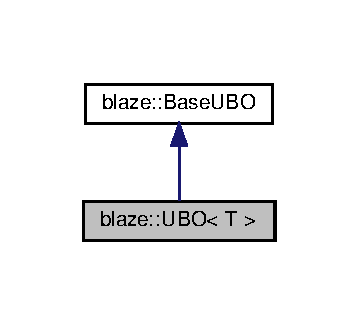
\includegraphics[width=172pt]{classblaze_1_1UBO__inherit__graph}
\end{center}
\end{figure}


Collaboration diagram for blaze\+:\+:U\+BO$<$ T $>$\+:\nopagebreak
\begin{figure}[H]
\begin{center}
\leavevmode
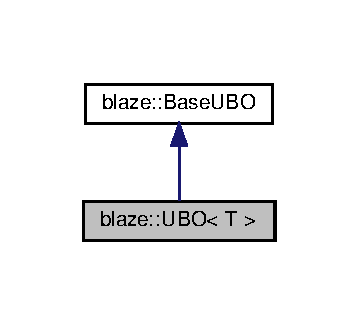
\includegraphics[width=172pt]{classblaze_1_1UBO__coll__graph}
\end{center}
\end{figure}
\subsection*{Public Member Functions}
\begin{DoxyCompactItemize}
\item 
\mbox{\Hypertarget{classblaze_1_1UBO_a23097bbba43a080b7ea2b99781896e6a}\label{classblaze_1_1UBO_a23097bbba43a080b7ea2b99781896e6a}} 
\hyperlink{classblaze_1_1UBO_a23097bbba43a080b7ea2b99781896e6a}{U\+BO} () noexcept
\begin{DoxyCompactList}\small\item\em Default Constructor. \end{DoxyCompactList}\item 
\hyperlink{classblaze_1_1UBO_a3df93d52c42c21080258f142862490bd}{U\+BO} (const \hyperlink{classblaze_1_1Context}{Context} $\ast$context, const T \&data) noexcept
\begin{DoxyCompactList}\small\item\em Main constructor of the class. \end{DoxyCompactList}\item 
void \hyperlink{classblaze_1_1UBO_a67e905adc995d3f0a8ec47208992674d}{write} (const T \&data)
\begin{DoxyCompactList}\small\item\em Writes the new data to the uniform buffer. \end{DoxyCompactList}\end{DoxyCompactItemize}
\subsection*{Additional Inherited Members}


\subsection{Detailed Description}
\subsubsection*{template$<$typename T$>$\newline
class blaze\+::\+U\+B\+O$<$ T $>$}

The class to handle operations on a uniform buffer. 


\begin{DoxyTemplParams}{Template Parameters}
{\em T} & The data object to be stored in the \hyperlink{classblaze_1_1UBO}{U\+BO}. \\
\hline
\end{DoxyTemplParams}


\subsection{Constructor \& Destructor Documentation}
\mbox{\Hypertarget{classblaze_1_1UBO_a3df93d52c42c21080258f142862490bd}\label{classblaze_1_1UBO_a3df93d52c42c21080258f142862490bd}} 
\index{blaze\+::\+U\+BO@{blaze\+::\+U\+BO}!U\+BO@{U\+BO}}
\index{U\+BO@{U\+BO}!blaze\+::\+U\+BO@{blaze\+::\+U\+BO}}
\subsubsection{\texorpdfstring{U\+B\+O()}{UBO()}}
{\footnotesize\ttfamily template$<$typename T$>$ \\
\hyperlink{classblaze_1_1UBO}{blaze\+::\+U\+BO}$<$ T $>$\+::\hyperlink{classblaze_1_1UBO}{U\+BO} (\begin{DoxyParamCaption}\item[{const \hyperlink{classblaze_1_1Context}{Context} $\ast$}]{context,  }\item[{const T \&}]{data }\end{DoxyParamCaption})\hspace{0.3cm}{\ttfamily [inline]}, {\ttfamily [noexcept]}}



Main constructor of the class. 


\begin{DoxyParams}{Parameters}
{\em context} & Pointer to the current Vulkan \hyperlink{classblaze_1_1Context}{Context}. \\
\hline
{\em data} & The data object of type T to store. \\
\hline
\end{DoxyParams}


\subsection{Member Function Documentation}
\mbox{\Hypertarget{classblaze_1_1UBO_a67e905adc995d3f0a8ec47208992674d}\label{classblaze_1_1UBO_a67e905adc995d3f0a8ec47208992674d}} 
\index{blaze\+::\+U\+BO@{blaze\+::\+U\+BO}!write@{write}}
\index{write@{write}!blaze\+::\+U\+BO@{blaze\+::\+U\+BO}}
\subsubsection{\texorpdfstring{write()}{write()}}
{\footnotesize\ttfamily template$<$typename T$>$ \\
void \hyperlink{classblaze_1_1UBO}{blaze\+::\+U\+BO}$<$ T $>$\+::write (\begin{DoxyParamCaption}\item[{const T \&}]{data }\end{DoxyParamCaption})\hspace{0.3cm}{\ttfamily [inline]}}



Writes the new data to the uniform buffer. 


\begin{DoxyParams}{Parameters}
{\em data} & The data to write to the uniform buffer. \\
\hline
\end{DoxyParams}


The documentation for this class was generated from the following file\+:\begin{DoxyCompactItemize}
\item 
Blaze/core/Uniform\+Buffer.\+hpp\end{DoxyCompactItemize}

\hypertarget{classblaze_1_1UBOVector}{}\section{blaze\+:\+:U\+B\+O\+Vector$<$ T $>$ Class Template Reference}
\label{classblaze_1_1UBOVector}\index{blaze\+::\+U\+B\+O\+Vector$<$ T $>$@{blaze\+::\+U\+B\+O\+Vector$<$ T $>$}}
\subsection*{Public Member Functions}
\begin{DoxyCompactItemize}
\item 
\mbox{\Hypertarget{classblaze_1_1UBOVector_a2eab32788ac1e58fe5f8da02ff720ec5}\label{classblaze_1_1UBOVector_a2eab32788ac1e58fe5f8da02ff720ec5}} 
{\bfseries U\+B\+O\+Vector} (const \hyperlink{classblaze_1_1Context}{Context} $\ast$context, const T \&data, uint32\+\_\+t num\+U\+B\+OS) noexcept
\item 
\mbox{\Hypertarget{classblaze_1_1UBOVector_aa2e1f83f1117b16e4777a203fa85a19a}\label{classblaze_1_1UBOVector_aa2e1f83f1117b16e4777a203fa85a19a}} 
{\bfseries U\+B\+O\+Vector} (const \hyperlink{classblaze_1_1UBOVector}{U\+B\+O\+Vector} \&other)=delete
\item 
\mbox{\Hypertarget{classblaze_1_1UBOVector_a25dcb4540c299af68e90e6562e638041}\label{classblaze_1_1UBOVector_a25dcb4540c299af68e90e6562e638041}} 
\hyperlink{classblaze_1_1UBOVector}{U\+B\+O\+Vector} \& {\bfseries operator=} (const \hyperlink{classblaze_1_1UBOVector}{U\+B\+O\+Vector} \&other)=delete
\item 
\mbox{\Hypertarget{classblaze_1_1UBOVector_af7c08e3af27268ed39c1427610e92321}\label{classblaze_1_1UBOVector_af7c08e3af27268ed39c1427610e92321}} 
{\bfseries U\+B\+O\+Vector} (\hyperlink{classblaze_1_1UBOVector}{U\+B\+O\+Vector} \&\&other)=default
\item 
\mbox{\Hypertarget{classblaze_1_1UBOVector_a3bdcee2bc412621221a82818fb00f665}\label{classblaze_1_1UBOVector_a3bdcee2bc412621221a82818fb00f665}} 
\hyperlink{classblaze_1_1UBOVector}{U\+B\+O\+Vector} \& {\bfseries operator=} (\hyperlink{classblaze_1_1UBOVector}{U\+B\+O\+Vector} \&\&other)=default
\item 
\mbox{\Hypertarget{classblaze_1_1UBOVector_aac87cae072ad7e35efe420426906282d}\label{classblaze_1_1UBOVector_aac87cae072ad7e35efe420426906282d}} 
const std\+::vector$<$ \hyperlink{classblaze_1_1UBO}{ubo\+\_\+t} $>$ \& {\bfseries get} () const
\item 
\mbox{\Hypertarget{classblaze_1_1UBOVector_a80d18385f477f31d26b6353afa2bfd99}\label{classblaze_1_1UBOVector_a80d18385f477f31d26b6353afa2bfd99}} 
uint32\+\_\+t {\bfseries size} () const
\item 
\mbox{\Hypertarget{classblaze_1_1UBOVector_a1c5ec068f74fcaf7cbf5ee80d7194349}\label{classblaze_1_1UBOVector_a1c5ec068f74fcaf7cbf5ee80d7194349}} 
\hyperlink{classblaze_1_1UBO}{ubo\+\_\+t} \& {\bfseries operator\mbox{[}$\,$\mbox{]}} (uint32\+\_\+t idx)
\item 
\mbox{\Hypertarget{classblaze_1_1UBOVector_ab8ed2d3a9fb0b23f32341795dc4e0879}\label{classblaze_1_1UBOVector_ab8ed2d3a9fb0b23f32341795dc4e0879}} 
const \hyperlink{classblaze_1_1UBO}{ubo\+\_\+t} \& {\bfseries operator\mbox{[}$\,$\mbox{]}} (uint32\+\_\+t idx) const
\end{DoxyCompactItemize}


The documentation for this class was generated from the following file\+:\begin{DoxyCompactItemize}
\item 
Blaze/core/Uniform\+Buffer.\+hpp\end{DoxyCompactItemize}

\hypertarget{structblaze_1_1spirv_1_1UniformInfo}{}\section{blaze\+:\+:spirv\+:\+:Uniform\+Info Struct Reference}
\label{structblaze_1_1spirv_1_1UniformInfo}\index{blaze\+::spirv\+::\+Uniform\+Info@{blaze\+::spirv\+::\+Uniform\+Info}}
\subsection*{Public Member Functions}
\begin{DoxyCompactItemize}
\item 
\mbox{\Hypertarget{structblaze_1_1spirv_1_1UniformInfo_a4d693bed4dd5b199d2b12094a5fdbe1c}\label{structblaze_1_1spirv_1_1UniformInfo_a4d693bed4dd5b199d2b12094a5fdbe1c}} 
bool {\bfseries operator!=} (const \hyperlink{structblaze_1_1spirv_1_1UniformInfo}{Uniform\+Info} \&other) const
\item 
\mbox{\Hypertarget{structblaze_1_1spirv_1_1UniformInfo_a66940ff24b7e8a54ef7d460f557c7a6f}\label{structblaze_1_1spirv_1_1UniformInfo_a66940ff24b7e8a54ef7d460f557c7a6f}} 
bool {\bfseries operator$<$} (const \hyperlink{structblaze_1_1spirv_1_1UniformInfo}{Uniform\+Info} \&other) const
\item 
\mbox{\Hypertarget{structblaze_1_1spirv_1_1UniformInfo_a769a3a96493a7a88593126719614af98}\label{structblaze_1_1spirv_1_1UniformInfo_a769a3a96493a7a88593126719614af98}} 
{\bfseries operator Vk\+Descriptor\+Set\+Layout\+Binding} ()
\end{DoxyCompactItemize}
\subsection*{Public Attributes}
\begin{DoxyCompactItemize}
\item 
\mbox{\Hypertarget{structblaze_1_1spirv_1_1UniformInfo_a291148732556d9f47dc09b5ed7650371}\label{structblaze_1_1spirv_1_1UniformInfo_a291148732556d9f47dc09b5ed7650371}} 
Vk\+Descriptor\+Type {\bfseries type}
\item 
\mbox{\Hypertarget{structblaze_1_1spirv_1_1UniformInfo_a57c673c1f65a2a3ec61023b3782c6129}\label{structblaze_1_1spirv_1_1UniformInfo_a57c673c1f65a2a3ec61023b3782c6129}} 
Vk\+Shader\+Stage\+Flags {\bfseries stages}
\item 
\mbox{\Hypertarget{structblaze_1_1spirv_1_1UniformInfo_afdbb99f3c149be3fe63f53e5220cf103}\label{structblaze_1_1spirv_1_1UniformInfo_afdbb99f3c149be3fe63f53e5220cf103}} 
uint32\+\_\+t {\bfseries binding}
\item 
\mbox{\Hypertarget{structblaze_1_1spirv_1_1UniformInfo_aef51d2d588169944d5c1dfcfe45e7e8c}\label{structblaze_1_1spirv_1_1UniformInfo_aef51d2d588169944d5c1dfcfe45e7e8c}} 
uint32\+\_\+t {\bfseries array\+Length}
\item 
\mbox{\Hypertarget{structblaze_1_1spirv_1_1UniformInfo_a472bc1a58d4a508b488dae87a2f39f66}\label{structblaze_1_1spirv_1_1UniformInfo_a472bc1a58d4a508b488dae87a2f39f66}} 
uint32\+\_\+t {\bfseries size}
\item 
\mbox{\Hypertarget{structblaze_1_1spirv_1_1UniformInfo_a08301c73e6e9d4e0ff6c935d07bb06e0}\label{structblaze_1_1spirv_1_1UniformInfo_a08301c73e6e9d4e0ff6c935d07bb06e0}} 
std\+::string {\bfseries name}
\end{DoxyCompactItemize}


The documentation for this struct was generated from the following file\+:\begin{DoxyCompactItemize}
\item 
Blaze/spirv/Pipeline.\+hpp\end{DoxyCompactItemize}

\hypertarget{classblaze_1_1util_1_1Unmanaged}{}\section{blaze\+:\+:util\+:\+:Unmanaged$<$ T $>$ Class Template Reference}
\label{classblaze_1_1util_1_1Unmanaged}\index{blaze\+::util\+::\+Unmanaged$<$ T $>$@{blaze\+::util\+::\+Unmanaged$<$ T $>$}}


A wrapper for handle for uniformity.  




{\ttfamily \#include $<$Managed.\+hpp$>$}

\subsection*{Public Member Functions}
\begin{DoxyCompactItemize}
\item 
\mbox{\Hypertarget{classblaze_1_1util_1_1Unmanaged_a5d9bf18bd244088eacfbd9222ffe4443}\label{classblaze_1_1util_1_1Unmanaged_a5d9bf18bd244088eacfbd9222ffe4443}} 
\hyperlink{classblaze_1_1util_1_1Unmanaged_a5d9bf18bd244088eacfbd9222ffe4443}{Unmanaged} () noexcept
\begin{DoxyCompactList}\small\item\em Default Constructor. \end{DoxyCompactList}\item 
\hyperlink{classblaze_1_1util_1_1Unmanaged_a1cd09eebfad8e92f75798127fb783f9d}{Unmanaged} (T handle) noexcept
\begin{DoxyCompactList}\small\item\em Main constructor. \end{DoxyCompactList}\item 
bool const \hyperlink{classblaze_1_1util_1_1Unmanaged_a945a30c97396b358cf250025520e9dbc}{valid} () const
\begin{DoxyCompactList}\small\item\em Checks validity of the handle. \end{DoxyCompactList}\end{DoxyCompactItemize}
\begin{Indent}\textbf{ Move Constructors.}\par
{\em Move only, copy deleted. }\begin{DoxyCompactItemize}
\item 
\mbox{\Hypertarget{classblaze_1_1util_1_1Unmanaged_a887c2d929464c22a9017506d8d252fde}\label{classblaze_1_1util_1_1Unmanaged_a887c2d929464c22a9017506d8d252fde}} 
{\bfseries Unmanaged} (\hyperlink{classblaze_1_1util_1_1Unmanaged}{Unmanaged} \&\&other) noexcept
\item 
\mbox{\Hypertarget{classblaze_1_1util_1_1Unmanaged_aca13c9955f89f999d35af547665f5021}\label{classblaze_1_1util_1_1Unmanaged_aca13c9955f89f999d35af547665f5021}} 
\hyperlink{classblaze_1_1util_1_1Unmanaged}{Unmanaged} \& {\bfseries operator=} (\hyperlink{classblaze_1_1util_1_1Unmanaged}{Unmanaged} \&\&other) noexcept
\item 
\mbox{\Hypertarget{classblaze_1_1util_1_1Unmanaged_a91256e8f121bae4a16ca982df6169fad}\label{classblaze_1_1util_1_1Unmanaged_a91256e8f121bae4a16ca982df6169fad}} 
{\bfseries Unmanaged} (const \hyperlink{classblaze_1_1util_1_1Unmanaged}{Unmanaged} \&other)=delete
\item 
\mbox{\Hypertarget{classblaze_1_1util_1_1Unmanaged_a348036688d4280d1a68797416f4d3097}\label{classblaze_1_1util_1_1Unmanaged_a348036688d4280d1a68797416f4d3097}} 
\hyperlink{classblaze_1_1util_1_1Unmanaged}{Unmanaged} \& {\bfseries operator=} (const \hyperlink{classblaze_1_1util_1_1Unmanaged}{Unmanaged} \&other)=delete
\end{DoxyCompactItemize}
\end{Indent}
\begin{Indent}\textbf{ Getters.}\par
{\em Getters for private fields. }\begin{DoxyCompactItemize}
\item 
\mbox{\Hypertarget{classblaze_1_1util_1_1Unmanaged_ac5ffb688acfa2843d62e644969cc0f8d}\label{classblaze_1_1util_1_1Unmanaged_ac5ffb688acfa2843d62e644969cc0f8d}} 
const T \& {\bfseries get} () const
\item 
\mbox{\Hypertarget{classblaze_1_1util_1_1Unmanaged_a8f0ece0ca74d59f42b396baed6b97483}\label{classblaze_1_1util_1_1Unmanaged_a8f0ece0ca74d59f42b396baed6b97483}} 
void {\bfseries set} (const T \&val)
\item 
\mbox{\Hypertarget{classblaze_1_1util_1_1Unmanaged_a2c4e1f19ec97030d6e83a108facb352d}\label{classblaze_1_1util_1_1Unmanaged_a2c4e1f19ec97030d6e83a108facb352d}} 
T $\ast$ {\bfseries data} ()
\end{DoxyCompactItemize}
\end{Indent}


\subsection{Detailed Description}
\subsubsection*{template$<$typename T$>$\newline
class blaze\+::util\+::\+Unmanaged$<$ T $>$}

A wrapper for handle for uniformity. 


\begin{DoxyTemplParams}{Template Parameters}
{\em T} & The type of handle wrapped. \\
\hline
\end{DoxyTemplParams}


\subsection{Constructor \& Destructor Documentation}
\mbox{\Hypertarget{classblaze_1_1util_1_1Unmanaged_a1cd09eebfad8e92f75798127fb783f9d}\label{classblaze_1_1util_1_1Unmanaged_a1cd09eebfad8e92f75798127fb783f9d}} 
\index{blaze\+::util\+::\+Unmanaged@{blaze\+::util\+::\+Unmanaged}!Unmanaged@{Unmanaged}}
\index{Unmanaged@{Unmanaged}!blaze\+::util\+::\+Unmanaged@{blaze\+::util\+::\+Unmanaged}}
\subsubsection{\texorpdfstring{Unmanaged()}{Unmanaged()}}
{\footnotesize\ttfamily template$<$typename T$>$ \\
\hyperlink{classblaze_1_1util_1_1Unmanaged}{blaze\+::util\+::\+Unmanaged}$<$ T $>$\+::\hyperlink{classblaze_1_1util_1_1Unmanaged}{Unmanaged} (\begin{DoxyParamCaption}\item[{T}]{handle }\end{DoxyParamCaption})\hspace{0.3cm}{\ttfamily [inline]}, {\ttfamily [noexcept]}}



Main constructor. 


\begin{DoxyParams}{Parameters}
{\em handle} & The handle. \\
\hline
\end{DoxyParams}


\subsection{Member Function Documentation}
\mbox{\Hypertarget{classblaze_1_1util_1_1Unmanaged_a945a30c97396b358cf250025520e9dbc}\label{classblaze_1_1util_1_1Unmanaged_a945a30c97396b358cf250025520e9dbc}} 
\index{blaze\+::util\+::\+Unmanaged@{blaze\+::util\+::\+Unmanaged}!valid@{valid}}
\index{valid@{valid}!blaze\+::util\+::\+Unmanaged@{blaze\+::util\+::\+Unmanaged}}
\subsubsection{\texorpdfstring{valid()}{valid()}}
{\footnotesize\ttfamily template$<$typename T$>$ \\
\hyperlink{classblaze_1_1util_1_1Unmanaged}{blaze\+::util\+::\+Unmanaged}$<$ T $>$\+::valid (\begin{DoxyParamCaption}{ }\end{DoxyParamCaption}) const\hspace{0.3cm}{\ttfamily [inline]}}



Checks validity of the handle. 

\begin{DoxyReturn}{Returns}
false if default constructed. 

true otherwise. 
\end{DoxyReturn}


The documentation for this class was generated from the following file\+:\begin{DoxyCompactItemize}
\item 
Blaze/util/Managed.\+hpp\end{DoxyCompactItemize}

\hypertarget{classblaze_1_1util_1_1UnmanagedVector}{}\section{blaze\+:\+:util\+:\+:Unmanaged\+Vector$<$ T $>$ Class Template Reference}
\label{classblaze_1_1util_1_1UnmanagedVector}\index{blaze\+::util\+::\+Unmanaged\+Vector$<$ T $>$@{blaze\+::util\+::\+Unmanaged\+Vector$<$ T $>$}}


Wrapper on vector of handles for consistency.  




{\ttfamily \#include $<$Managed.\+hpp$>$}

\subsection*{Public Member Functions}
\begin{DoxyCompactItemize}
\item 
\mbox{\Hypertarget{classblaze_1_1util_1_1UnmanagedVector_ae2e722d08c5247bceff137c73e7447d6}\label{classblaze_1_1util_1_1UnmanagedVector_ae2e722d08c5247bceff137c73e7447d6}} 
\hyperlink{classblaze_1_1util_1_1UnmanagedVector_ae2e722d08c5247bceff137c73e7447d6}{Unmanaged\+Vector} () noexcept
\begin{DoxyCompactList}\small\item\em Default Constructor. \end{DoxyCompactList}\item 
\mbox{\Hypertarget{classblaze_1_1util_1_1UnmanagedVector_a3a2030e5b1f1e1b3fd7d083d2d17d798}\label{classblaze_1_1util_1_1UnmanagedVector_a3a2030e5b1f1e1b3fd7d083d2d17d798}} 
\hyperlink{classblaze_1_1util_1_1UnmanagedVector_a3a2030e5b1f1e1b3fd7d083d2d17d798}{Unmanaged\+Vector} (const std\+::vector$<$ T $>$ \&handles) noexcept
\begin{DoxyCompactList}\small\item\em Copies the handles for construction. \end{DoxyCompactList}\item 
\mbox{\Hypertarget{classblaze_1_1util_1_1UnmanagedVector_a13a25be3b436be664beb83b13c3f1378}\label{classblaze_1_1util_1_1UnmanagedVector_a13a25be3b436be664beb83b13c3f1378}} 
\hyperlink{classblaze_1_1util_1_1UnmanagedVector_a13a25be3b436be664beb83b13c3f1378}{Unmanaged\+Vector} (std\+::vector$<$ T $>$ \&\&handles) noexcept
\begin{DoxyCompactList}\small\item\em Moves the handles for construction. \end{DoxyCompactList}\item 
bool \hyperlink{classblaze_1_1util_1_1UnmanagedVector_a13e031e44e8ddfa77492bedbf1c82780}{valid} () const
\begin{DoxyCompactList}\small\item\em Returns the validity of the construction. \end{DoxyCompactList}\end{DoxyCompactItemize}
\begin{Indent}\textbf{ Move Constructors.}\par
{\em Move only, copy deleted. }\begin{DoxyCompactItemize}
\item 
\mbox{\Hypertarget{classblaze_1_1util_1_1UnmanagedVector_adde99e03709712a5555c769ccaa93ecc}\label{classblaze_1_1util_1_1UnmanagedVector_adde99e03709712a5555c769ccaa93ecc}} 
{\bfseries Unmanaged\+Vector} (\hyperlink{classblaze_1_1util_1_1UnmanagedVector}{Unmanaged\+Vector} \&\&other) noexcept
\item 
\mbox{\Hypertarget{classblaze_1_1util_1_1UnmanagedVector_a071f358ea12fa14456483fdd63d6d8c5}\label{classblaze_1_1util_1_1UnmanagedVector_a071f358ea12fa14456483fdd63d6d8c5}} 
\hyperlink{classblaze_1_1util_1_1UnmanagedVector}{Unmanaged\+Vector} \& {\bfseries operator=} (\hyperlink{classblaze_1_1util_1_1UnmanagedVector}{Unmanaged\+Vector} \&\&other) noexcept
\item 
\mbox{\Hypertarget{classblaze_1_1util_1_1UnmanagedVector_a854f58df88590cb705768eb408ab7f4a}\label{classblaze_1_1util_1_1UnmanagedVector_a854f58df88590cb705768eb408ab7f4a}} 
{\bfseries Unmanaged\+Vector} (const \hyperlink{classblaze_1_1util_1_1UnmanagedVector}{Unmanaged\+Vector} \&other)=delete
\item 
\mbox{\Hypertarget{classblaze_1_1util_1_1UnmanagedVector_a58ff760293fd63e1eaa84d2fddb93a2d}\label{classblaze_1_1util_1_1UnmanagedVector_a58ff760293fd63e1eaa84d2fddb93a2d}} 
\hyperlink{classblaze_1_1util_1_1UnmanagedVector}{Unmanaged\+Vector} \& {\bfseries operator=} (const \hyperlink{classblaze_1_1util_1_1UnmanagedVector}{Unmanaged\+Vector} \&other)=delete
\end{DoxyCompactItemize}
\end{Indent}
\begin{Indent}\textbf{ Getters.}\par
{\em Getters for private members. }\begin{DoxyCompactItemize}
\item 
\mbox{\Hypertarget{classblaze_1_1util_1_1UnmanagedVector_a3676adcb36f6c460b77d58d066d86920}\label{classblaze_1_1util_1_1UnmanagedVector_a3676adcb36f6c460b77d58d066d86920}} 
const std\+::vector$<$ T $>$ \& {\bfseries get} () const
\item 
\mbox{\Hypertarget{classblaze_1_1util_1_1UnmanagedVector_aeb328d698db37ac813e6977914d38208}\label{classblaze_1_1util_1_1UnmanagedVector_aeb328d698db37ac813e6977914d38208}} 
const T \& {\bfseries get} (size\+\_\+t index) const
\item 
\mbox{\Hypertarget{classblaze_1_1util_1_1UnmanagedVector_a786430b2b037993cd3996a5c73f2a2cb}\label{classblaze_1_1util_1_1UnmanagedVector_a786430b2b037993cd3996a5c73f2a2cb}} 
void {\bfseries set} (size\+\_\+t index, const T \&val)
\item 
\mbox{\Hypertarget{classblaze_1_1util_1_1UnmanagedVector_a12fee5564f693695745f8c98c852c13b}\label{classblaze_1_1util_1_1UnmanagedVector_a12fee5564f693695745f8c98c852c13b}} 
T \& {\bfseries operator\mbox{[}$\,$\mbox{]}} (size\+\_\+t index)
\item 
\mbox{\Hypertarget{classblaze_1_1util_1_1UnmanagedVector_a0309e57150e45c3fd801aae55d423a5c}\label{classblaze_1_1util_1_1UnmanagedVector_a0309e57150e45c3fd801aae55d423a5c}} 
const T \& {\bfseries operator\mbox{[}$\,$\mbox{]}} (size\+\_\+t index) const
\item 
\mbox{\Hypertarget{classblaze_1_1util_1_1UnmanagedVector_aab508ac9a2288fa20915e2f3025a1afd}\label{classblaze_1_1util_1_1UnmanagedVector_aab508ac9a2288fa20915e2f3025a1afd}} 
T $\ast$ {\bfseries data} ()
\item 
\mbox{\Hypertarget{classblaze_1_1util_1_1UnmanagedVector_a3565245fa593d9928acac754d353ca33}\label{classblaze_1_1util_1_1UnmanagedVector_a3565245fa593d9928acac754d353ca33}} 
void {\bfseries resize} (size\+\_\+t size)
\item 
\mbox{\Hypertarget{classblaze_1_1util_1_1UnmanagedVector_a7df456122f8074b1029f713b33586954}\label{classblaze_1_1util_1_1UnmanagedVector_a7df456122f8074b1029f713b33586954}} 
size\+\_\+t {\bfseries size} () const
\end{DoxyCompactItemize}
\end{Indent}


\subsection{Detailed Description}
\subsubsection*{template$<$typename T$>$\newline
class blaze\+::util\+::\+Unmanaged\+Vector$<$ T $>$}

Wrapper on vector of handles for consistency. 


\begin{DoxyTemplParams}{Template Parameters}
{\em T} & Type of the handle. \\
\hline
\end{DoxyTemplParams}


\subsection{Member Function Documentation}
\mbox{\Hypertarget{classblaze_1_1util_1_1UnmanagedVector_a13e031e44e8ddfa77492bedbf1c82780}\label{classblaze_1_1util_1_1UnmanagedVector_a13e031e44e8ddfa77492bedbf1c82780}} 
\index{blaze\+::util\+::\+Unmanaged\+Vector@{blaze\+::util\+::\+Unmanaged\+Vector}!valid@{valid}}
\index{valid@{valid}!blaze\+::util\+::\+Unmanaged\+Vector@{blaze\+::util\+::\+Unmanaged\+Vector}}
\subsubsection{\texorpdfstring{valid()}{valid()}}
{\footnotesize\ttfamily template$<$typename T $>$ \\
\hyperlink{classblaze_1_1util_1_1UnmanagedVector}{blaze\+::util\+::\+Unmanaged\+Vector}$<$ T $>$\+::valid (\begin{DoxyParamCaption}{ }\end{DoxyParamCaption}) const\hspace{0.3cm}{\ttfamily [inline]}}



Returns the validity of the construction. 

\begin{DoxyReturn}{Returns}
false if default constructed. 

true otherwise. 
\end{DoxyReturn}


The documentation for this class was generated from the following file\+:\begin{DoxyCompactItemize}
\item 
Blaze/util/Managed.\+hpp\end{DoxyCompactItemize}

\hypertarget{structblaze_1_1Vertex}{}\section{blaze\+:\+:Vertex Struct Reference}
\label{structblaze_1_1Vertex}\index{blaze\+::\+Vertex@{blaze\+::\+Vertex}}


\hyperlink{structblaze_1_1Vertex}{Vertex} type commonly used with interleaved data.  




{\ttfamily \#include $<$Datatypes.\+hpp$>$}

\subsection*{Static Public Member Functions}
\begin{DoxyCompactItemize}
\item 
static Vk\+Vertex\+Input\+Binding\+Description \hyperlink{structblaze_1_1Vertex_a81e9b6e602df735ad45fcc5d2c3305c6}{get\+Binding\+Description} (uint32\+\_\+t binding=0)
\begin{DoxyCompactList}\small\item\em Creates and returns the binding description for the \hyperlink{structblaze_1_1Vertex}{Vertex}. \end{DoxyCompactList}\item 
static std\+::vector$<$ Vk\+Vertex\+Input\+Attribute\+Description $>$ \hyperlink{structblaze_1_1Vertex_aa9ee165c3cfdac311ca8ffc382524d4b}{get\+Attribute\+Descriptions} (\hyperlink{structblaze_1_1VertexInputFormat}{Vertex\+Input\+Format} format=\{\}, uint32\+\_\+t binding=0)
\begin{DoxyCompactList}\small\item\em Creates attribute descriptions for the vertex. \end{DoxyCompactList}\end{DoxyCompactItemize}
\subsection*{Public Attributes}
\begin{DoxyCompactItemize}
\item 
\mbox{\Hypertarget{structblaze_1_1Vertex_a1e1592274327ef0a3c655b85826af54b}\label{structblaze_1_1Vertex_a1e1592274327ef0a3c655b85826af54b}} 
glm\+::vec3 \hyperlink{structblaze_1_1Vertex_a1e1592274327ef0a3c655b85826af54b}{position}
\begin{DoxyCompactList}\small\item\em Position of the vertex. \end{DoxyCompactList}\item 
\mbox{\Hypertarget{structblaze_1_1Vertex_ab0bb46f8b4ffc80a6c622e629401a5fd}\label{structblaze_1_1Vertex_ab0bb46f8b4ffc80a6c622e629401a5fd}} 
glm\+::vec3 \hyperlink{structblaze_1_1Vertex_ab0bb46f8b4ffc80a6c622e629401a5fd}{normal}
\begin{DoxyCompactList}\small\item\em Normal vector outwards from the vertex. \end{DoxyCompactList}\item 
\mbox{\Hypertarget{structblaze_1_1Vertex_acc8d9d8254c0515edad905e50126ce2b}\label{structblaze_1_1Vertex_acc8d9d8254c0515edad905e50126ce2b}} 
glm\+::vec2 \hyperlink{structblaze_1_1Vertex_acc8d9d8254c0515edad905e50126ce2b}{uv0}
\begin{DoxyCompactList}\small\item\em Texture Coordinate (0) \end{DoxyCompactList}\item 
\mbox{\Hypertarget{structblaze_1_1Vertex_afee0041ee5ef260ac1418119a2b132e5}\label{structblaze_1_1Vertex_afee0041ee5ef260ac1418119a2b132e5}} 
glm\+::vec2 \hyperlink{structblaze_1_1Vertex_afee0041ee5ef260ac1418119a2b132e5}{uv1}
\begin{DoxyCompactList}\small\item\em Texture Coordinate (1) \end{DoxyCompactList}\end{DoxyCompactItemize}


\subsection{Detailed Description}
\hyperlink{structblaze_1_1Vertex}{Vertex} type commonly used with interleaved data. 

\subsection{Member Function Documentation}
\mbox{\Hypertarget{structblaze_1_1Vertex_aa9ee165c3cfdac311ca8ffc382524d4b}\label{structblaze_1_1Vertex_aa9ee165c3cfdac311ca8ffc382524d4b}} 
\index{blaze\+::\+Vertex@{blaze\+::\+Vertex}!get\+Attribute\+Descriptions@{get\+Attribute\+Descriptions}}
\index{get\+Attribute\+Descriptions@{get\+Attribute\+Descriptions}!blaze\+::\+Vertex@{blaze\+::\+Vertex}}
\subsubsection{\texorpdfstring{get\+Attribute\+Descriptions()}{getAttributeDescriptions()}}
{\footnotesize\ttfamily blaze\+::\+Vertex\+::get\+Attribute\+Descriptions (\begin{DoxyParamCaption}\item[{\hyperlink{structblaze_1_1VertexInputFormat}{Vertex\+Input\+Format}}]{format = {\ttfamily \{\}},  }\item[{uint32\+\_\+t}]{binding = {\ttfamily 0} }\end{DoxyParamCaption})\hspace{0.3cm}{\ttfamily [inline]}, {\ttfamily [static]}}



Creates attribute descriptions for the vertex. 


\begin{DoxyParams}[1]{Parameters}
\mbox{\tt in}  & {\em format} & The binding locations for each of the vertex inputs. \\
\hline
\mbox{\tt in}  & {\em binding} & Binding location of the vertex attribute.\\
\hline
\end{DoxyParams}
\begin{DoxyReturn}{Returns}
vector of attribute descriptions 
\end{DoxyReturn}
\mbox{\Hypertarget{structblaze_1_1Vertex_a81e9b6e602df735ad45fcc5d2c3305c6}\label{structblaze_1_1Vertex_a81e9b6e602df735ad45fcc5d2c3305c6}} 
\index{blaze\+::\+Vertex@{blaze\+::\+Vertex}!get\+Binding\+Description@{get\+Binding\+Description}}
\index{get\+Binding\+Description@{get\+Binding\+Description}!blaze\+::\+Vertex@{blaze\+::\+Vertex}}
\subsubsection{\texorpdfstring{get\+Binding\+Description()}{getBindingDescription()}}
{\footnotesize\ttfamily blaze\+::\+Vertex\+::get\+Binding\+Description (\begin{DoxyParamCaption}\item[{uint32\+\_\+t}]{binding = {\ttfamily 0} }\end{DoxyParamCaption})\hspace{0.3cm}{\ttfamily [inline]}, {\ttfamily [static]}}



Creates and returns the binding description for the \hyperlink{structblaze_1_1Vertex}{Vertex}. 


\begin{DoxyParams}[1]{Parameters}
\mbox{\tt in}  & {\em binding} & Binding location of the vertex attribute.\\
\hline
\end{DoxyParams}
\begin{DoxyReturn}{Returns}
\hyperlink{structblaze_1_1Vertex}{Vertex} Input Binding Description 
\end{DoxyReturn}


The documentation for this struct was generated from the following file\+:\begin{DoxyCompactItemize}
\item 
Blaze/Datatypes.\+hpp\end{DoxyCompactItemize}

\hypertarget{classblaze_1_1VertexBuffer}{}\section{blaze\+:\+:Vertex\+Buffer$<$ T $>$ Class Template Reference}
\label{classblaze_1_1VertexBuffer}\index{blaze\+::\+Vertex\+Buffer$<$ T $>$@{blaze\+::\+Vertex\+Buffer$<$ T $>$}}


Object encapsulating the data in a vertex buffer.  




{\ttfamily \#include $<$Vertex\+Buffer.\+hpp$>$}



Inheritance diagram for blaze\+:\+:Vertex\+Buffer$<$ T $>$\+:\nopagebreak
\begin{figure}[H]
\begin{center}
\leavevmode
\includegraphics[width=205pt]{classblaze_1_1VertexBuffer__inherit__graph}
\end{center}
\end{figure}


Collaboration diagram for blaze\+:\+:Vertex\+Buffer$<$ T $>$\+:\nopagebreak
\begin{figure}[H]
\begin{center}
\leavevmode
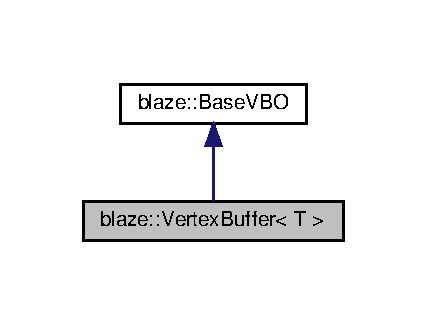
\includegraphics[width=205pt]{classblaze_1_1VertexBuffer__coll__graph}
\end{center}
\end{figure}
\subsection*{Public Member Functions}
\begin{DoxyCompactItemize}
\item 
\mbox{\Hypertarget{classblaze_1_1VertexBuffer_af1ee16f904c7f531dfd3f0cd14f9b89b}\label{classblaze_1_1VertexBuffer_af1ee16f904c7f531dfd3f0cd14f9b89b}} 
\hyperlink{classblaze_1_1VertexBuffer_af1ee16f904c7f531dfd3f0cd14f9b89b}{Vertex\+Buffer} () noexcept
\begin{DoxyCompactList}\small\item\em Default Constructor. \end{DoxyCompactList}\item 
\hyperlink{classblaze_1_1VertexBuffer_a6852238a5dfe856d9cee5532498ecdcc}{Vertex\+Buffer} (const \hyperlink{classblaze_1_1Context}{Context} $\ast$context, const std\+::vector$<$ T $>$ \&data) noexcept
\begin{DoxyCompactList}\small\item\em Main constructor. \end{DoxyCompactList}\item 
\mbox{\Hypertarget{classblaze_1_1VertexBuffer_acd64f1e4e28aefee16fb3a720d0490cd}\label{classblaze_1_1VertexBuffer_acd64f1e4e28aefee16fb3a720d0490cd}} 
void {\bfseries bind} (Vk\+Command\+Buffer buf) const
\end{DoxyCompactItemize}
\subsection*{Additional Inherited Members}


\subsection{Detailed Description}
\subsubsection*{template$<$typename T$>$\newline
class blaze\+::\+Vertex\+Buffer$<$ T $>$}

Object encapsulating the data in a vertex buffer. 


\begin{DoxyTemplParams}{Template Parameters}
{\em T} & The type of vertex data held by the buffer. \\
\hline
\end{DoxyTemplParams}


\subsection{Constructor \& Destructor Documentation}
\mbox{\Hypertarget{classblaze_1_1VertexBuffer_a6852238a5dfe856d9cee5532498ecdcc}\label{classblaze_1_1VertexBuffer_a6852238a5dfe856d9cee5532498ecdcc}} 
\index{blaze\+::\+Vertex\+Buffer@{blaze\+::\+Vertex\+Buffer}!Vertex\+Buffer@{Vertex\+Buffer}}
\index{Vertex\+Buffer@{Vertex\+Buffer}!blaze\+::\+Vertex\+Buffer@{blaze\+::\+Vertex\+Buffer}}
\subsubsection{\texorpdfstring{Vertex\+Buffer()}{VertexBuffer()}}
{\footnotesize\ttfamily template$<$typename T$>$ \\
\hyperlink{classblaze_1_1VertexBuffer}{blaze\+::\+Vertex\+Buffer}$<$ T $>$\+::\hyperlink{classblaze_1_1VertexBuffer}{Vertex\+Buffer} (\begin{DoxyParamCaption}\item[{const \hyperlink{classblaze_1_1Context}{Context} $\ast$}]{context,  }\item[{const std\+::vector$<$ T $>$ \&}]{data }\end{DoxyParamCaption})\hspace{0.3cm}{\ttfamily [inline]}, {\ttfamily [noexcept]}}



Main constructor. 


\begin{DoxyParams}{Parameters}
{\em context} & The Vulkan \hyperlink{classblaze_1_1Context}{Context} in use. \\
\hline
{\em data} & A vector of vertices ({\itshape T}) to be held in the buffer. \\
\hline
\end{DoxyParams}


The documentation for this class was generated from the following file\+:\begin{DoxyCompactItemize}
\item 
Blaze/core/Vertex\+Buffer.\+hpp\end{DoxyCompactItemize}

\hypertarget{structblaze_1_1VertexInputFormat}{}\section{blaze\+:\+:Vertex\+Input\+Format Struct Reference}
\label{structblaze_1_1VertexInputFormat}\index{blaze\+::\+Vertex\+Input\+Format@{blaze\+::\+Vertex\+Input\+Format}}


Descriptes the input arrangement for the Vertex\+Input stage.  




{\ttfamily \#include $<$Datatypes.\+hpp$>$}

\subsection*{Public Member Functions}
\begin{DoxyCompactItemize}
\item 
\hyperlink{structblaze_1_1VertexInputFormat_a303f81c990469ace47c11051105434fe}{Vertex\+Input\+Format} ()
\begin{DoxyCompactList}\small\item\em Default Constructor. \end{DoxyCompactList}\end{DoxyCompactItemize}
\subsection*{Public Attributes}
\begin{DoxyCompactItemize}
\item 
\mbox{\Hypertarget{structblaze_1_1VertexInputFormat_a667c06a846b60712be75b98463d59827}\label{structblaze_1_1VertexInputFormat_a667c06a846b60712be75b98463d59827}} 
uint32\+\_\+t \hyperlink{structblaze_1_1VertexInputFormat_a667c06a846b60712be75b98463d59827}{A\+\_\+\+P\+O\+S\+I\+T\+I\+ON}
\begin{DoxyCompactList}\small\item\em The location of the position attribute of a vertex. \end{DoxyCompactList}\item 
\mbox{\Hypertarget{structblaze_1_1VertexInputFormat_a3c1e00b7012a2993f4316fa603dc4f01}\label{structblaze_1_1VertexInputFormat_a3c1e00b7012a2993f4316fa603dc4f01}} 
uint32\+\_\+t \hyperlink{structblaze_1_1VertexInputFormat_a3c1e00b7012a2993f4316fa603dc4f01}{A\+\_\+\+N\+O\+R\+M\+AL}
\begin{DoxyCompactList}\small\item\em The location of the normal attribute of a vertex. \end{DoxyCompactList}\item 
\mbox{\Hypertarget{structblaze_1_1VertexInputFormat_a174031ae8fa572a5a6df7340d192c702}\label{structblaze_1_1VertexInputFormat_a174031ae8fa572a5a6df7340d192c702}} 
uint32\+\_\+t \hyperlink{structblaze_1_1VertexInputFormat_a174031ae8fa572a5a6df7340d192c702}{A\+\_\+\+U\+V0}
\begin{DoxyCompactList}\small\item\em The location of the UV coordinate set 0 attribute of a vertex. \end{DoxyCompactList}\item 
\mbox{\Hypertarget{structblaze_1_1VertexInputFormat_ab5cf84ff3d8787836792c9a4ca4bfd46}\label{structblaze_1_1VertexInputFormat_ab5cf84ff3d8787836792c9a4ca4bfd46}} 
uint32\+\_\+t \hyperlink{structblaze_1_1VertexInputFormat_ab5cf84ff3d8787836792c9a4ca4bfd46}{A\+\_\+\+U\+V1}
\begin{DoxyCompactList}\small\item\em The location of the UV coordinate set 1 attribute of a vertex. \end{DoxyCompactList}\end{DoxyCompactItemize}


\subsection{Detailed Description}
Descriptes the input arrangement for the Vertex\+Input stage. 

The format is used to properly assign the inputs to match in inputs in the \hyperlink{structblaze_1_1Vertex}{Vertex} Shader. 

\subsection{Constructor \& Destructor Documentation}
\mbox{\Hypertarget{structblaze_1_1VertexInputFormat_a303f81c990469ace47c11051105434fe}\label{structblaze_1_1VertexInputFormat_a303f81c990469ace47c11051105434fe}} 
\index{blaze\+::\+Vertex\+Input\+Format@{blaze\+::\+Vertex\+Input\+Format}!Vertex\+Input\+Format@{Vertex\+Input\+Format}}
\index{Vertex\+Input\+Format@{Vertex\+Input\+Format}!blaze\+::\+Vertex\+Input\+Format@{blaze\+::\+Vertex\+Input\+Format}}
\subsubsection{\texorpdfstring{Vertex\+Input\+Format()}{VertexInputFormat()}}
{\footnotesize\ttfamily blaze\+::\+Vertex\+Input\+Format\+::\+Vertex\+Input\+Format (\begin{DoxyParamCaption}{ }\end{DoxyParamCaption})\hspace{0.3cm}{\ttfamily [inline]}}



Default Constructor. 

The default constructor initializes the attributes to their default ascending order. 

The documentation for this struct was generated from the following file\+:\begin{DoxyCompactItemize}
\item 
Blaze/Datatypes.\+hpp\end{DoxyCompactItemize}

%--- End generated contents ---

% Index
\backmatter
\newpage
\phantomsection
\clearemptydoublepage
\addcontentsline{toc}{chapter}{Index}
\printindex

\end{document}
